\documentclass[11pt,oneside]{book}
\usepackage{fontspec}
\usepackage[CJKspace]{xeCJK}
\setmainfont{Latin Modern Roman}
\setCJKmainfont[ItalicFont={Noto Serif CJK KR},BoldItalicFont={Noto Serif CJK KR Bold}]{Noto Serif CJK KR}
\setCJKsansfont{Noto Sans CJK KR}
\setCJKmonofont{Noto Sans Mono CJK KR}
\newfontfamily\proseunicodefont{DejaVu Serif}
\usepackage[margin=1in]{geometry}
\usepackage{microtype}
\usepackage{amsmath,amssymb,amsthm,mathtools,bm}
\usepackage{graphicx}
\usepackage{adjustbox}
\usepackage{xcolor}
\usepackage{booktabs}
\usepackage{array}
\usepackage{longtable}
\usepackage{enumitem}
\usepackage{float}
\usepackage{caption}
\usepackage{hyperref}
\usepackage{fancyhdr}
\usepackage{tikz}
\usetikzlibrary{arrows.meta,positioning,calc,decorations.pathmorphing}

\hypersetup{
  colorlinks=true,
  linkcolor=blue!50!black,
  urlcolor=blue!50!black,
  citecolor=blue!50!black
}

\setlength{\parskip}{0.5em}
\setlength{\parindent}{0pt}
\setlist[itemize]{topsep=0.25em,itemsep=0.2em}
\setlist[enumerate]{topsep=0.25em,itemsep=0.2em}
\setlength{\headheight}{40pt}
\numberwithin{equation}{chapter}

\newtheorem{theorem}{정리}[chapter]
\newtheorem{proposition}[theorem]{명제}
\newtheorem{lemma}[theorem]{보조정리}
\newtheorem{corollary}[theorem]{따름정리}
\theoremstyle{definition}
\newtheorem{definition}[theorem]{정의}
\newtheorem{example}[theorem]{예}
\theoremstyle{remark}
\newtheorem{remark}[theorem]{비고}

\providecommand{\ket}[1]{\left\lvert#1\right\rangle}
\providecommand{\bra}[1]{\left\langle#1\right\rvert}
\providecommand{\braket}[2]{\left\langle#1\,\middle|\,#2\right\rangle}
\providecommand{\expect}[1]{\left\langle#1\right\rangle}
\newcommand{\lectureoverview}[1]{\paragraph{개요.} #1}
\newenvironment{classroomqa}{%
  \par\medskip
  \begin{minipage}{0.96\textwidth}
}{%
  \end{minipage}
  \par\medskip
}
\newcommand{\audiencequestion}[1]{\noindent\textbf{청중 질문.} #1\par\smallskip}
\newcommand{\lecturerresponse}[1]{\noindent\textbf{답변.} #1\par}
\newcommand{\lecturetimestamp}[1]{\footnote{강의 시각: #1.}}
\newcommand{\lectureframe}[1]{\par\smallskip{\centering\footnotesize\itshape 강의 화면: #1.\par}}
\newcommand{\editorialnote}[1]{\footnote{편집자 설명: #1}}

\makeatletter
\newcommand{\course@headerfont}{\normalfont\small\itshape}
\newcommand{\course@pagefont}{\normalfont\small}
\newcommand{\course@headerraise}{14pt}
\newlength{\course@headerboxheight}
\setlength{\course@headerboxheight}{\dimexpr\headheight-\course@headerraise-9pt\relax}
\newcommand{\course@leftheadbox}[1]{%
  \raisebox{\course@headerraise}{%
    \parbox[t][\course@headerboxheight][t]{0.82\textwidth}{%
      \raggedright\course@headerfont\strut\MakeUppercase{#1}\strut%
    }%
  }%
}
\newcommand{\course@rightheadbox}[1]{%
  \raisebox{\course@headerraise}{%
    \parbox[t][\course@headerboxheight][t]{0.82\textwidth}{%
      \raggedleft\course@headerfont\strut\MakeUppercase{#1}\strut%
    }%
  }%
}
\renewcommand{\chaptermark}[1]{\markboth{\MakeUppercase{\chaptername\ \thechapter.\ #1}}{}}
\renewcommand{\sectionmark}[1]{\markright{\MakeUppercase{\thesection\hspace{0.4em}#1}}}
\fancyhf{}
\fancyhead[L]{\course@leftheadbox{\leftmark}}
\fancyhead[R]{\course@pagefont\thepage}
\renewcommand{\headrulewidth}{0.5pt}
\pagestyle{fancy}
\fancypagestyle{plain}{%
  \fancyhf{}
  \fancyhead[L]{\course@leftheadbox{\leftmark}}
  \fancyhead[R]{\course@pagefont\thepage}
  \renewcommand{\headrulewidth}{0.5pt}
}
\makeatother

\renewcommand{\contentsname}{목차}
\renewcommand{\chaptername}{장}
\renewcommand{\figurename}{그림}
\renewcommand{\tablename}{표}
\renewcommand{\proofname}{증명}
\renewcommand{\bibname}{참고문헌}
\emergencystretch=2em
\pdfstringdefDisableCommands{\def\proseunicodefont{}}

\geometry{paperwidth=177.6mm,paperheight=252mm,left=16mm,right=16mm,
 top=18mm,bottom=18mm,includeheadfoot,headheight=28pt,headsep=7mm,footskip=9mm}
\usepackage{scrextend}
\changefontsizes[17pt]{12pt}
\raggedbottom
\renewenvironment{classroomqa}{\par\medskip\begingroup}{\par\endgroup\medskip}
\fancyhf{}
\setlength{\headwidth}{\textwidth}
\fancyhead[L]{\parbox{\textwidth}{\raggedright\fontsize{9}{11}\selectfont\nouppercase{\leftmark}}}
\fancyfoot[C]{\small\thepage}
\renewcommand{\headrulewidth}{0.3pt}
\fancypagestyle{plain}{\fancyhf{}\fancyfoot[C]{\small\thepage}\renewcommand{\headrulewidth}{0pt}}

\graphicspath{{../../../generated_course_notes/supplementary/string_theory/2010_fall_string_theory_and_m_theory/figures/}{../../../generated_course_notes/supplementary/string_theory/2010_fall_string_theory_and_m_theory/assets/}}
\begin{document}
\frontmatter
\hypersetup{pageanchor=false}
\begin{titlepage}
\hyphenpenalty=10000\exhyphenpenalty=10000
\thispagestyle{empty}
\begin{tikzpicture}[remember picture,overlay]
  \node[anchor=center,inner sep=0] at (current page.center) {%
    \includegraphics[height=\paperheight,keepaspectratio]{../../../generated_course_notes/supplementary/string_theory/2010_fall_string_theory_and_m_theory/assets/cover-art.png}%
  };
  \node[
    anchor=north west,
    align=left,
    text width=0.78\paperwidth,
    fill=white,
    fill opacity=0.9,
    rounded corners=8pt,
    inner xsep=10pt,
    inner ysep=8pt
  ] at ([xshift=0.08\paperwidth,yshift=-0.06\paperheight]current page.north west) {%
    {\fontsize{30}{33}\selectfont\bfseries\color{black!88} 끈 이론과 M이론\\[0.85em]}
    {\large\color{black!72} 한국어판 / 2010년 가을 · 끈 이론과 M이론}
  };
  \node[
    anchor=south west,
    align=left,
    text width=0.68\paperwidth,
    fill=white,
    fill opacity=0.82,
    text opacity=1,
    rounded corners=6pt,
    inner sep=12pt
  ] at ([xshift=0.08\paperwidth,yshift=0.08\paperheight]current page.south west) {%
    {\normalsize\color{black!78} 원 강의: Leonard Susskind\\[0.35em]}
    {\small\color{black!72} 보조 강의 노트: \href{https://lazying.art}{LazyingArt LLC} / \href{https://github.com/lachlanchen/Video2Book}{Video2Book}}
  };
\end{tikzpicture}
\mbox{}
\end{titlepage}
\hypersetup{pageanchor=true}

\clearpage
\chapter{이 노트에 대하여}
이 보충 노트는 Leonard Susskind의 강의를 바탕으로 독립적으로 편집한 자료입니다. 기계 생성 전사문과 자막, 일부 칠판 화면을 토대로 재구성한 뒤, 확인 가능한 원자료와 대조해 검토했습니다. 이 자료는 Susskind 교수의 원고가 아니며, 교수의 검토나 승인을 받지 않았습니다.

이 판본은 \href{https://lazying.art}{LazyingArt LLC}가 오픈 소스 \href{https://github.com/lachlanchen/Video2Book}{Video2Book} 워크플로를 사용해 제작했습니다. 기계 생성 전사문은 별도로 제공되며, 음성 인식 오류가 있을 수 있습니다. 편집 과정에서 추가한 설명과 실질적인 재구성은 각주에 표시했습니다.
\clearpage
\tableofcontents
\mainmatter
\chapter{하드론 레제 궤적에서 광원뿔 끈까지}

\lectureoverview{끈 이론은 양자 중력 이론으로 시작하지 않았다.
하드론의 스펙트럼과 산란을 이해하려는 시도에서 출발했다.
직선 레제 궤적은 확장된 물체를 시사했고,
파이온--파이온 산란의 쌍대성은 겉보기에 서로 다른 두 과정이 하나의 표면을 서로 다르게 자른 결과일 수 있음을 시사했다. 이 단서들을 따라 세계면 그림으로 나아가고, 하드론 끈을 QCD 플럭스 튜브로 재해석한 다음, 무한운동량계에서 열린 끈의 횡방향 역학을 유도해 보자.
핵심 결과는 유효 내부 해밀토니안이 질량 제곱을 측정한다는 것이다. 따라서 그 기술에서 \(L^2\)에 비례하는 훅의 법칙 형태의 에너지는 \(L\)에 비례하는 정지 에너지가 되며, 이것이 일정한 장력을 가진 끈의 특징적인 거동이다.}

\section{끈 이론의 하드론 기원}

1968--1970 무렵 끈 이론의 단초가 된 문제는 양성자, 중성자, 특히 중간자와 관련되어 있었다. 쿼크 모형은 이미 진지하게 고려되는 아이디어였지만, 오늘날의 의미에서 하드론의 쿼크 구성이 실험적으로 확립된 것은 아니었다. 글루온은 일반적인 논의에서 훨씬 덜 두드러졌다. 남부는 관련된 게이지장 아이디어를 제안했지만, 양자색역학이라는 정립된 언어는 아직 존재하지 않았다. 당시의 출발점은 오히려 강하게 상호작용하는 입자들이 보여 준 예상 밖으로 풍부한 스펙트럼이었다.

잠시 양성자--중성자 구분을 접어 두고 두 상태를 모두 핵자라고 부르면 편리하다. 핵자보다 무거운 상태들 가운데는 스핀이 더 큰 상태들이 있었고, 그 뒤로는 더 무거우면서 스핀도 더 큰 상태들이 이어졌다. 츄와 프라우치(Chew와 Frautschi)는 세로축에 각운동량, 가로축에 질량 제곱을 놓은 그래프에 이런 계열을 정리했다. 당시의 단위로 양성자 질량은 약 1 BeV였으며, 이 단위는 오늘날 GeV라고 불린다.

각운동량을 \(\hbar\) 단위로 측정하자. 중입자 계열에서 무차원 스핀 값은 반정수이다.

\begin{equation}
  J=\frac12,\frac32,\frac52,\ldots,
\end{equation}

반면 중간자 계열의 스핀은 정수이다. 놀라운 경험적 사실은 어느 계열이든 \(M^2\)에 대해 그래프로 나타내면 대략 직선 위에 놓인다는 점이었다. 현대 표기법으로는 다음과 같이 쓴다.

\begin{equation}
  J\simeq \alpha_0+\alpha' M^2,
  \label{eq:l01-regge-trajectory}
\end{equation}

여기서 \(\alpha_0\)은 절편이고 \(\alpha'\)는 레제 기울기이다.
\editorialnote{강의에서는 관측된 선형 관계와 거의 보편적인 기울기를 강조한다. 절편 표기는 이 관계를 간결하게 나타내기 위해 제시한 것이며, 궤적은 경험적으로 얻은 근삿값이다.}

처음 발견된 직선 자체는 알려진 두 점만 지났기 때문에 설득력이 크지 않았다. 어떤 두 점도 직선 하나를 정하기 때문이다. 놀라운 점은 이후에 새로 발견된 상태들도 계속 같은 직선 가까이에 놓였다는 사실이었다. 중간자 궤적도 같은 구조를 보였다. 파이온은 \(J=0\)에서 시작하며 GeV 규모로 질량이 작고, 로는 \(J=1\)에서 시작한다. 더 높은 여기 상태들도 계속 이어진다. 한 계열에 입자가 다섯, 여섯, 일곱 개 나타나기도 했다. 더욱 놀라운 점은 서로 다른 중입자와 중간자 궤적들이 거의 평행했다는 것이다. 따라서 각운동량이 양자 하나만큼 증가할 때 질량 제곱도 대략 같은 양만큼 증가했다.

\begin{equation}
  \Delta J=1
  \quad\Longrightarrow\quad
  \Delta M^2\simeq \frac{1}{\alpha'}.
  \label{eq:l01-regge-spacing}
\end{equation}

\begin{classroomqa}
\audiencequestion{서로 다른 레제 궤적이 평행하다는 것은 무슨 뜻인가요?\lecturetimestamp{00:09:32}}
\lecturerresponse{입자 계열 하나를 골라 여기 상태들을 모두 그래프로 나타내면 한 직선 위에 놓입니다. 다른 중간자 또는 중입자 계열에 대해서도 같은 작업을 해 보세요. 절편은 달라도 직선들의 기울기는 대략 같습니다. 따라서 각운동량의 같은 증가량에는 \(M^2\)의 증가량도 대략 같게 듭니다. 이 공통 기울기를 보편적 레제 기울기라고 불렀습니다.}
\end{classroomqa}

일반적인 확장 물체와 비교하면 이 패턴이 왜 중요했는지 알 수 있다. 농구공을 회전시키면 회전 에너지가 증가하지만, 궤적은 직선이 아니라 곡선이며 각속도가 충분히 커지면 공은 찢어진다. 원자에도 회전 여기가 있지만, 결국 이온화되어 궤적이 끝난다. 하드론에서는 훨씬 단순한 계열이 나타났고, 당시 얻을 수 있는 자료에서는 그 계열이 끝나려는 기미가 보이지 않았다.

이 스펙트럼은 하드론이 점입자처럼 거동하지 않는다는 것을 보여 주었다. 점입자에는 회전하거나 변형할 공간 구조가 없다. 전자에서는 더 높은 스핀을 가진 내부 상태의 탑이 관측되지 않았으며, 이에 따라 현재 실험 한계 안에서는 점입자로 여겨진다. 반면 하드론은 회전 속도를 높일 수 있다. 그 스펙트럼은 하드론이 복합체임을 시사하고, 스핀과 질량의 관계는 각운동량이 커질수록 물체가 변형됨을 암시한다.

\section{파이온--파이온 산란에서의 쌍대성}

분광학에서 하나의 단서를 얻었다. 파이온--파이온 산란에서도 또 다른 단서를 얻었다. 두 파이온은 로와 비슷한 공명 상태를 이루었다가 나중에 다시 두 파이온으로 나올 수 있다. 표준 파인만 도표에서는 이것이 소멸과 재생성 과정이며, 관례적으로 \(s\)-채널 과정이라 부른다. 같은 기본 도표를 옆으로 돌려 보면 교차된 \(t\)-채널 과정이 되며, 이 경우 로와 비슷한 입자가 두 파이온 사이에서 교환된다.

로만 있는 것은 아니다. 로는 레제 계열에 속하므로, 두 채널 어느 쪽에서든 로와 모든 여기 동반 상태가 포함되어야 할 것처럼 보인다. 개략적으로 쓰면 다음과 같다.

\begin{equation}
  \mathcal A(s,t)\simeq
  \sum_n \mathcal A^{(s)}_{\rho_n}(s,t),
  \qquad
  \mathcal A(s,t)\simeq
  \sum_n \mathcal A^{(t)}_{\rho_n}(s,t).
  \label{eq:l01-channel-sums}
\end{equation}

이 식들은 단순히 더해야 하는 두 근사가 아니다. 수치 연구에 따르면 소멸 채널에서 공명 상태 탑을 합산하는 것만으로도 교환 채널에서 예상되는 기여를 대략 얻을 수 있었다. 반대로 교환 상태들의 탑으로도 공명 상태 기술을 재현할 수 있었다. 따라서 두 탑 전체를 더하면 같은 물리를 두 번 세는 셈인 듯했다. 일반적인 섭동론의 계산 규칙에 따르면 도표가 두 개 있으면 둘 다 포함해야 한다. 그러나 하드론 산란 진폭은 두 채널 기술이 쌍대임을 시사했다.

\begin{figure}[H]
  \centering
  \includegraphics[width=0.82\textwidth]{lecture_01_figure_01.png}
  \caption{칠판에는 츄--프라우치 그래프와 소멸 및 교차 채널 도표가 함께 그려져 있어, 스펙트럼과 산란의 단서가 하나의 문제로 연결된다.}
  \lectureframe{00:14:20}
  \label{fig:l01-regge-duality-board}
\end{figure}

같은 관계를 간결한 개략도로 분리해 나타낼 수 있다. 첫 번째 패널은 선형 스펙트럼을 나타내고, 나머지 두 패널은 동일한 산란 진폭을 채널별로 전개하는 서로 다른 방식을 나타낸다.

\begin{figure}[H]
  \centering
  \resizebox{\textwidth}{!}{%
  \begin{tikzpicture}[>=Latex,thick]
    \begin{scope}
      \draw[->] (0,0) -- (4.2,0) node[right] {$M^2$};
      \draw[->] (0,0) -- (0,3.4) node[above] {$J$};
      \draw[blue!65!black] (0.45,0.35) -- (3.55,2.95);
      \draw[orange!80!black] (0.75,0.20) -- (3.85,2.80);
      \foreach \x/\y in {0.65/0.52,1.35/1.10,2.05/1.69,2.75/2.27,3.45/2.86}
        \fill[blue!65!black] (\x,\y) circle (0.07);
      \foreach \x/\y in {0.95/0.37,1.65/0.95,2.35/1.54,3.05/2.12,3.75/2.71}
        \fill[orange!80!black] (\x,\y) circle (0.07);
      \node at (2.1,-0.55) {parallel Regge families};
    \end{scope}
    \begin{scope}[xshift=5.7cm]
      \draw[->] (-1.5,1.2) -- (-0.3,0.25);
      \draw[->] (-1.5,-1.2) -- (-0.3,-0.25);
      \draw[decorate,decoration={snake,amplitude=1.5pt,segment length=7pt}]
        (0,0.25) -- (0,-0.25);
      \draw[->] (0.3,0.25) -- (1.5,1.2);
      \draw[->] (0.3,-0.25) -- (1.5,-1.2);
      \node at (0,-1.75) {$s$-channel tower};
    \end{scope}
    \begin{scope}[xshift=10.5cm]
      \draw[->] (-1.5,1.2) -- (1.5,1.2);
      \draw[->] (-1.5,-1.2) -- (1.5,-1.2);
      \draw[decorate,decoration={snake,amplitude=1.5pt,segment length=7pt}]
        (0,0.95) -- (0,-0.95);
      \node at (0,-1.75) {$t$-channel tower};
    \end{scope}
  \end{tikzpicture}}
  \caption{평행한 레제 계열과 하드론 쌍대성에 관련된 두 채널 전개.}
  \label{fig:l01-regge-duality-redraw}
\end{figure}

\section{하나의 세계면, 두 가지 단면}

자연스러운 대응은 두 가지 방식으로 읽을 수 있는 하나의 기하학적 역사를 찾는 것이었다. 파이온을 쿼크--반쿼크 쌍으로 나타내고 시간을 위쪽으로 흐르게 하자. 입자의 1차원 궤적만 그리는 대신 쿼크의 궤적이 둘러싸는 영역을 채워 넣는다. 이 2차원 역사를 수평으로 자르면 두 개의 들어오는 끈이 합쳐졌다가 다시 갈라지는 모습을 볼 수 있다. 다른 방향으로 자르면 한쪽에서 다른 쪽으로 교환되는 끈이 나타난다. 두 파인만 채널 그림은 더 이상 서로 독립적인 메커니즘이 아니라, 하나의 표면을 서로 다르게 분해해 기술한 결과다.

\begin{figure}[H]
  \centering
  \includegraphics[width=0.78\textwidth]{lecture_01_figure_02.png}
  \caption{칠판에 그린 쿼크 선의 위상. 동일한 2차원 역사를 서로 다르게 자르면 공명과 교환이라는 두 가지 해석이 나온다.}
  \lectureframe{00:17:50}
  \label{fig:l01-worldsheet-topology-board}
\end{figure}

쿼크와 반쿼크 사이의 영역에서 한 가지 아이디어가 더 나온다. 특정 시각의 단면에는 양 끝점 둘과 그 사이의 구간 전체를 채우는 무언가가 있다. 그것은 1차원 물체, 즉 끈이다. 상호작용 중에 끈은 2차원 표면을 쓸고 지나간다.

\begin{definition}
점입자의 시공간 역사는 \emph{세계선}이다. 끈의 시공간 역사는 \emph{세계면}이다. 한 순간의 끈은 그 세계면을 공간적으로 자른 단면이다.
\end{definition}

\begin{figure}[H]
  \centering
  \includegraphics[width=0.78\textwidth]{lecture_01_figure_03.png}
  \caption{끝점 궤적 사이를 채운 칠판의 표면. 시간 단면은 이 표면을 가로질러 1차원 끈을 이룬다.}
  \lectureframe{00:19:15}
  \label{fig:l01-worldsheet-filled-board}
\end{figure}

\begin{figure}[H]
  \centering
  \begin{tikzpicture}[>=Latex,scale=0.95]
    \fill[blue!10]
      (-2.6,-2.3) .. controls (-1.0,-1.0) and (-1.0,-0.4) .. (-0.2,0)
      .. controls (-1.0,0.5) and (-1.0,1.0) .. (-2.6,2.3)
      -- (2.6,2.3)
      .. controls (1.0,1.0) and (1.0,0.5) .. (0.2,0)
      .. controls (1.0,-0.4) and (1.0,-1.0) .. (2.6,-2.3) -- cycle;
    \draw[blue!65!black]
      (-2.6,-2.3) .. controls (-1.0,-1.0) and (-1.0,-0.4) .. (-0.2,0)
      .. controls (-1.0,0.5) and (-1.0,1.0) .. (-2.6,2.3);
    \draw[blue!65!black]
      (2.6,-2.3) .. controls (1.0,-1.0) and (1.0,-0.4) .. (0.2,0)
      .. controls (1.0,0.5) and (1.0,1.0) .. (2.6,2.3);
    \draw[red!75!black,dashed] (-2.9,-1.15) -- (2.9,-1.15)
      node[right] {time slice};
    \draw[orange!80!black,dashed] (-1.55,-2.5) -- (1.55,2.5)
      node[above] {crossed slicing};
    \draw[->] (3.45,-1.7) -- (3.45,1.8) node[above] {time};
    \node[blue!65!black] at (0,-2.7) {one world sheet};
  \end{tikzpicture}
  \caption{세계면을 깔끔하게 나타낸 개략도. 서로 다른 단면은 동일한 표면을 서로 다른 중간 채널 기술로 정리한다.}
  \label{fig:l01-worldsheet-redraw}
\end{figure}

이러한 기하학적 재구성은 탐색적 시도였으며, 제1원리에서 완전한 이론을 연역한 것은 아니었다. 사람마다 초기 끈 그림에 도달한 경로는 달랐다. 이 그림의 강점은 하나의 확장된 물체가 두 관측 결과를 모두 설명할 수 있다는 데 있었다. 끈은 회전하고 변형될 수 있으며, 그 세계면은 쌍대 산란 채널을 부호화할 수 있다.

\begin{classroomqa}
\audiencequestion{쿼크 사이를 보통의 교환 입자로 연결하는 대신 끈 같은 다리를 도입하는 이유는 무엇인가요?\lecturetimestamp{00:21:20}}
\lecturerresponse{한순간에 국소화된 교환 입자만 있는 것이 아닙니다. 쿼크와 반쿼크가 있고, 그 사이의 모든 지점에도 구조가 있습니다. 그 구조가 근본적으로 연속적인지, 아니면 연속체를 근사하는 조밀한 구성 요소들의 집합인지는 첫 그림에서 결정되지 않았습니다. 중요한 점은 구간 전체가 채워져 있고, 관측된 궤적이 양 끝에 추를 단 보통의 구두끈처럼 끝나는 경향을 보이지 않았다는 것입니다.}
\end{classroomqa}

\begin{classroomqa}
\audiencequestion{표준 모형으로 파이온 산란을 설명할 수 있나요?
\lecturetimestamp{00:22:45}}
\lecturerresponse{네, 다만 유용성은 에너지 영역에 따라 달라집니다. 낮은 에너지에서는 QCD와 그 저에너지 기술을 통해 표준 모형이 파이온 산란의 상당 부분을 설명합니다. 여러 하드론 교환 상태들의 탑이 중요한 고에너지에서는 직접 계산이 더 어려워지며, 끈과 같은 체계로 정리하는 편이 더 유용할 수 있습니다.}
\end{classroomqa}

\begin{classroomqa}
\audiencequestion{초기 실험으로 레제 궤적이 끝나지 않는다는 사실이 확립되었나요?\lecturetimestamp{00:23:37}}
\lecturerresponse{아닙니다. 관측된 계열에서 아직 끝점이 나타나지 않았다는 사실만 확인되었습니다. 무한히 늘어날 수 있다는 추론은 시사적인 외삽이지, 무한대를 측정한 결과가 아닙니다.}
\end{classroomqa}

\section{플럭스 튜브와 규모의 변화}

현대 QCD는 오래된 그림에 장론적 해석을 부여한다. 쿼크와 반쿼크는 글루온장의 서로 반대인 원천으로 작용한다. 일반적인 전기역학에서는 전하를 서로 떼어 놓을수록 전기 플럭스가 옆으로 퍼진다. 거리가 멀어지면 장이 약해지므로 전하 사이 영역은 일정한 횡방향 분포를 유지하지 않는다. QCD는 비선형 이론이다. 그 동역학은 관련된 색전기 플럭스를 쿼크와 반쿼크를 잇는 가느다란 튜브 안에 가둘 수 있다.

\begin{figure}[H]
  \centering
  \includegraphics[width=0.78\textwidth]{lecture_01_figure_04.png}
  \caption{자유롭게 퍼지는 쿨롱 장이 아니라 가느다란 플럭스 튜브로 그린 쿼크와 반쿼크의 장선.}
  \lectureframe{00:25:15}
  \label{fig:l01-qcd-flux-board}
\end{figure}

\begin{figure}[H]
  \centering
  \begin{tikzpicture}[>=Latex]
    \fill[orange!14,rounded corners=8pt] (-3.0,-0.55) rectangle (3.0,0.55);
    \draw[orange!80!black,thick,rounded corners=8pt]
      (-3.0,-0.55) rectangle (3.0,0.55);
    \fill[blue!70!black] (-3.35,0) circle (0.17);
    \fill[red!75!black] (3.35,0) circle (0.17);
    \node[below] at (-3.35,-0.22) {$q$};
    \node[below] at (3.35,-0.22) {$\bar q$};
    \foreach \y in {-0.30,0,0.30}
      \draw[->,orange!85!black] (-3.05,\y) -- (3.05,\y);
    \draw[<->] (-2.9,-1.05) -- (2.9,-1.05) node[midway,below] {$L$};
    \node at (0,0.92) {approximately fixed transverse profile};
  \end{tikzpicture}
  \caption{가둔 플럭스 튜브는 퍼지지 않은 채 길어진다. 길이 단위당 에너지가 일정하면 \(E=TL\)가 된다.}
  \label{fig:l01-qcd-flux-redraw}
\end{figure}

입자에 관한 언어와 장에 관한 언어는 같은 내용을 다르게 말한다. 장 기술에서는 양 끝점 사이의 거리가 벌어져도 튜브가 대략 같은 장 세기와 단면적을 유지한다. 구성 요소 그림에서는 늘어날 때 생기는 에너지가 양 끝점 사이에 더 많은 글루온 구조를 만들어 낸다. 일반적인 고무줄은 분자 수가 일정하므로 분자들이 서로 멀어지다가 재료가 끊어진다. 틈이 벌어질 때마다 새 분자가 하나씩 끼워진다고 상상해 보자. 그러면 고무줄이 길어져도 길이 방향의 밀도는 일정하게 유지될 수 있다. 이것이 글루온장에 빗댄 의도다. 튜브는 끊어지기 직전까지 가늘어지는 대신 길이를 늘린다.

\begin{classroomqa}
\audiencequestion{전자를 이루는 끈도 글루온으로 구성되나요?\lecturetimestamp{00:28:08}}
\lecturerresponse{그런 결론은 나오지 않습니다. 하드론 끈은 양성자 규모의 QCD 물체입니다. 양자 중력과 관련된 가설상의 기본 끈은 훨씬 작은 플랑크 규모에 존재하며, 전자가 하드론 글루온 끈이라는 증거는 없습니다. 놀라운 사실은 두 규모에서 관련된 수학이 나타났다는 것이지, 물리적 대상들이 동일하다는 것이 아닙니다.}
\end{classroomqa}

강입자 그림을 완전한 상호작용 끈 이론으로 발전시키려는 시도는 유망했지만, 강입자 이론으로서 바라던 이론을 완전히 만들어 내지는 못했다. 수학적 모형에는 질량이 없는 스핀 2 입자가 거듭 등장했다. 강입자 이론에서는 이 상태가 원치 않는 예측처럼 보였지만, 중력 이론에서는 중력자와 양자수가 정확히 일치했다. 조엘 셰르크와 존 슈바르츠는 결정적인 재해석을 했다. 어쩌면 이 이론은 강입자가 아니라 양자 중력에 관해 말해 주고 있었던 것일 수 있다. 초기 강입자 문제는 수학으로 가는 길을 제공했지만, 강입자 이론과 기본 이론으로서의 응용은 물리적으로 서로 다르다.

\begin{classroomqa}
\audiencequestion{플럭스 선은 양의 끝점에서 음의 끝점으로 어떻게 이어지나요?\lecturetimestamp{00:31:46}}
\lecturerresponse{막대자석의 자기력선이 북극에서 남극으로 향하듯, 한 원천에서 나와 다른 원천으로 들어갑니다. 양 끝점의 반대 표지는 플럭스의 방향을 나타냅니다. 막대자석에도 북극 두 개가 아니라 서로 반대인 두 극이 있습니다.}
\end{classroomqa}

\begin{classroomqa}
\audiencequestion{끈은 연속적인가요, 아니면 이산적인가요?
\lecturetimestamp{00:32:45}}
\lecturerresponse{양자 이론에서는 이 구분이 미묘합니다. 전자기장은 연속장으로 표현되지만 이산적인 양자도 가집니다. 마찬가지로 끈은 연속적으로 다룰 수 있고, 그 여기 상태는 양자화됩니다. 어떤 질문을 하는지에 따라 두 기술 모두 유효할 수 있습니다.}
\end{classroomqa}

\begin{classroomqa}
\audiencequestion{세계면을 가로지르는 시공간 단면의 각도를 바꾸어도 교차선은 여전히 끈인가요?\lecturetimestamp{00:34:20}}
\lecturerresponse{네. 동시성 단면을 바꾸는 것은 로런츠 변환입니다. 새 단면은 표면과 교차하여 운동 상태가 다르게 보이는 끈을 만듭니다. 질량중심이 정지해 있는 끈도 내부까지 정지한 것은 아니며, 진동할 수 있습니다. ``정지''라는 말은 질량중심에 대해서만 가리킵니다.}
\end{classroomqa}

\section{상대론적 에너지의 두 가지 전개}

확장되어 진동하는 물체를 상대론적으로 직접 기술하기는 까다롭다. 유용한 전략은 관련 운동이 보통의 비상대론적 역학 형태를 띠는 기준계를 찾는 것이다. 먼저 단일 입자에서 시작하자. 비상대론적으로는 다음과 같이 쓴다.

\begin{equation}
  E_{\mathrm{nr}}=\frac{\bm p^2}{2m}+B,
  \label{eq:l01-nonrel-energy}
\end{equation}

여기서 \(B\)는 전체 운동량과 무관한 내부 에너지 또는 결합 에너지다. 상호작용하지 않는 입자가 여러 개라면 운동 에너지 항과 내부 상수 항을 각각 더한다. 운동을 결정하는 것은 에너지 차이뿐이므로, 상태에 무관한 가산 상수는 흔히 생략할 수 있다.

정확한 상대론적 에너지는 다음과 같다.

\begin{equation}
  E=\sqrt{\bm p^2c^2+m^2c^4}.
  \label{eq:l01-rel-energy-c}
\end{equation}

\begin{figure}[H]
  \centering
  \includegraphics[width=0.76\textwidth]{lecture_01_figure_05.png}
  \caption{비상대론적 운동 에너지와 정확한 상대론적 제곱근. 논의 중 바로잡은 \(c\)의 거듭제곱을 반영했다.}
  \lectureframe{00:38:45}
  \label{fig:l01-relativistic-energy-board}
\end{figure}

\begin{classroomqa}
\audiencequestion{상대론적 공식에는 칠판에 처음 쓴 거듭제곱 대신 \(p^2c^2\)와
\(m^2c^4\)가 들어가야 하나요?
\lecturetimestamp{00:39:12}}
\lecturerresponse{네. 차원 일관성을 고려하면 식은 \(E^2=p^2c^2+m^2c^4\)이어야 합니다. 비상대론적 극한을 얻은 다음에는 \(c=1\)로 놓겠지만, 여기서 거듭제곱을 그대로 두면 전개가 어떻게 되는지 분명히 보입니다.}
\end{classroomqa}

\(p^2c^2\ll m^2c^4\)일 때, \(m^2c^4\)를 인수로 묶고 다음을 이용한다:
\(\sqrt{1+\epsilon}\simeq1+\epsilon/2\)

\begin{align}
  E
  &=mc^2\sqrt{1+\frac{p^2}{m^2c^2}}
  \notag\\
  &\simeq mc^2+\frac{p^2}{2m}.
  \label{eq:l01-low-momentum-expansion}
\end{align}

\begin{figure}[H]
  \centering
  \includegraphics[width=0.76\textwidth]{lecture_01_figure_06.png}
  \caption{작은 운동량 전개를 통해 정지 에너지와 익숙한 비상대론적 운동 에너지가 나온다.}
  \lectureframe{00:41:30}
  \label{fig:l01-low-momentum-board}
\end{figure}

이 근사가 성립하려면 질량중심의 운동이 느리기만 해서는 부족하다. 상자 자체는 천천히 움직여도 내부 입자들은 빛의 속도에 가깝게 움직일 수 있다. 이 경우 내부 동역학은 여전히 상대론적이다. 보통의 비상대론적 극한이 성립하려면 선택한 기준계에서 모든 관련 구성 입자의 속도가 작아야 한다.

또 다른 유용한 극한이 있다. 전체 계를 \(z\)축 방향으로 부스트하여 모든 구성 입자가 큰 양의 종방향 운동량 \(P_{zi}\)을 갖게 한다. 처음에 뒤로 움직이던 구성 입자도 충분히 큰 부스트를 가하면 앞으로 움직이게 된다. 횡방향 운동량과 정지 질량은 그대로 유지된다.

\begin{equation}
  P_{zi}\gg |p_{xi}|,|p_{yi}|,m_i,
  \qquad
  p_{\perp i}^2=p_{xi}^2+p_{yi}^2,
\end{equation}

이제부터는 \(c=1\)로 놓는다. 큰 \(P_{zi}\)에 대해 전개하면 다음을 얻는다.

\begin{align}
  E_i
  &=\sqrt{P_{zi}^2+p_{\perp i}^2+m_i^2}
  \notag\\
  &=P_{zi}\sqrt{1+\frac{p_{\perp i}^2+m_i^2}{P_{zi}^2}}
  \notag\\
  &\simeq P_{zi}
  +\frac{p_{\perp i}^2+m_i^2}{2P_{zi}}.
  \label{eq:l01-large-pz-one-particle}
\end{align}

\begin{figure}[H]
  \centering
  \includegraphics[width=0.76\textwidth]{lecture_01_figure_07.png}
  \caption{큰 \(P_z\)에 대한 제곱근 전개. 횡방향 운동량과 질량은 작은 양으로 남겨 둔다.}
  \lectureframe{00:46:45}
  \label{fig:l01-large-pz-board}
\end{figure}

구성 입자가 여러 개일 때는 다음과 같다.

\begin{equation}
  E\simeq
  \sum_i P_{zi}
  +\sum_i\frac{p_{\perp i}^2}{2P_{zi}}
  +\sum_i\frac{m_i^2}{2P_{zi}}.
  \label{eq:l01-large-pz-sum}
\end{equation}

첫 번째 항은 보존되는 전체 종방향 운동량이다. 이 값은 매우 크지만 고정된 가산 기여이기도 하다. 이를 유지하거나 빼도 에너지 차이는 변하지 않는다. 해밀토니안에 다른 보존량을 더해도 운동 방정식이 바뀌지 않는 것과 같다. 따라서 동역학을 나타내는 부분은 다음과 같다.

\begin{equation}
  \begin{aligned}
    H_{\perp}=E-P_z
    &\simeq
    \sum_i\left(
      \frac{p_{\perp i}^2}{2P_{zi}}
      +\frac{m_i^2}{2P_{zi}}
    \right),\\
    P_z&=\sum_iP_{zi}.
  \end{aligned}
  \label{eq:l01-transverse-hamiltonian}
\end{equation}

\begin{figure}[H]
  \centering
  \includegraphics[width=0.78\textwidth]{lecture_01_figure_08.png}
  \caption{여러 입자의 항을 보존되는 종방향 운동량, 횡방향 운동 에너지, 질량에 따른 내부 항으로 분해한 식.}
  \lectureframe{00:49:16}
  \label{fig:l01-energy-sum-board}
\end{figure}

\section{무한운동량계}

앞에서 살펴본 극한은 역사적으로 무한운동량계라고 불렸으며, 오늘날에는 보통 광원뿔 좌표를 이용해 정식화한다. 해밀토니안에서 그 의미를 직접 읽을 수 있다. 양자역학에서는

\begin{equation}
  i\hbar\frac{\partial}{\partial t}\ket{\psi}=H\ket{\psi}.
  \label{eq:l01-time-evolution}
\end{equation}

\(H_{\perp}\)의 모든 비자명한 항은 \(1/P_z\)의 크기만큼 스케일한다. 부스트가 커질수록 에너지 준위 차이는 줄고 변화는 더 느려진다. 이것이 시간 지연이다. 방사성 계는 큰 부스트를 받으면 붕괴가 더 느려지는 것처럼 보이며, 그에 비례해 더 오랫동안 관측하면 이를 보정할 수 있다. 느려져도 동역학이 사라지는 것은 아니다. 동역학의 시계가 재조정되는 것이다.

\begin{figure}[H]
  \centering
  \includegraphics[width=0.78\textwidth]{lecture_01_figure_09.png}
  \caption{칠판에서는 감소된 에너지를 부스트된 계의 느려진 시간 변화를 일으키는 해밀토니안으로 본다.}
  \lectureframe{00:52:57}
  \label{fig:l01-hamiltonian-board}
\end{figure}

횡방향 항은 정확히 비상대론적 형태인 \(p^2/(2m)\)를 띠지만, 질량의 역할은 \(P_z\)가 맡는다. 이는 물리적으로 타당하다. 종방향 운동량이 클수록 입자의 옆 방향 편향이 어려워지므로 횡방향 관성처럼 작용한다. 항 \(m_i^2/(2P_{zi})\)는 2차원 운동 상태에 의존하지 않으므로 내부 에너지 또는 결합 에너지 역할을 한다. 3차원 공간의 상대론적 운동은 부스트에 수직인 두 차원에서 비상대론적으로 보이는 운동이 된다.

이제 상대론적 끈에 질량과 용수철로 이루어진 간단한 모형을 사용할 수 있다. 이 모형은 끈이 정지계에서 느리게 움직인다고 가정하는 것이 아니다. 횡방향 동역학이 필요한 비상대론적 구조를 갖는 기준계를 이용하는 것이다.

\section{구슬과 용수철로 만든 열린 끈}

열린 끈, 즉 끝점이 두 개인 끈을 생각하자. 나중에 그 끝점에 무언가를 붙일 수 있지만, 지금은 끈 자체에 관심을 둔다. 횡방향 위치 \(\bm X_i(t)=(X_i(t),Y_i(t))\)에 구슬을 놓고 동일한 용수철로 연결해 근사한다. 이산 해밀토니안은 다음과 같다.

\begin{equation}
  H_N=\sum_{i=1}^{N}
  \left[
    \frac{\mu_N}{2}\dot{\bm X}_i^{\,2}
    +\frac{k_N}{2}
      \left(\bm X_{i+1}-\bm X_i\right)^2
  \right].
  \label{eq:l01-discrete-string}
\end{equation}

운동 에너지만 있으면 구슬들은 서로 멀어져 날아간다. 최근접 이웃 사이의 훅 항이 있어야 구슬들이 끈을 이룬다.

\begin{figure}[H]
  \centering
  \includegraphics[width=0.75\textwidth]{lecture_01_figure_10.png}
  \caption{횡방향 좌표 두 개를 가진 열린 끈을 구슬과 용수철로 처음 나타낸 그림.}
  \lectureframe{01:00:30}
  \label{fig:l01-bead-chain-board}
\end{figure}

\begin{figure}[H]
  \centering
  \begin{tikzpicture}[>=Latex]
    \foreach \x in {0,...,8} {
      \fill[blue!65!black] ({0.85*\x},0) circle (0.09);
    }
    \foreach \x in {0,...,7} {
      \draw[decorate,decoration={zigzag,segment length=4pt,amplitude=2pt}]
        ({0.85*\x+0.10},0) -- ({0.85*\x+0.75},0);
    }
    \draw[->] (3.4,0.15) -- (3.4,1.25) node[above] {$\bm X_i(t)$};
    \draw[<->] (0,-0.65) -- (6.8,-0.65)
      node[midway,below] {$0\leq\sigma\leq\pi$};
  \end{tikzpicture}
  \caption{열린 끈의 이산 조절자. 연속체 극한을 취하기 전에 구슬 질량과 용수철 상수를 간격에 따라 스케일한다.}
  \label{fig:l01-bead-chain-redraw}
\end{figure}

\begin{figure}[H]
  \centering
  \includegraphics[width=0.78\textwidth]{lecture_01_figure_11.png}
  \caption{연속체 극한을 취하기 전에 이산 운동 에너지 항과 훅 항을 함께 쓴 식.}
  \lectureframe{01:01:30}
  \label{fig:l01-discrete-energy-board}
\end{figure}

구슬의 수가 늘어날수록 각 구슬의 질량 \(\mu_N\)는 0으로 가야 끈 전체의 관성이 유한하게 유지된다. 동시에 용수철 상수 \(k_N\)는 커져야 한다. 같은 재료의 짧은 조각보다 긴 고무 띠를 일정한 길이만큼 늘리는 편이 쉽다. 따라서 연속체 재료를 그대로 유지하려면 서로 가까워지는 이웃 점들을 더 강하게 연결해야 한다.

끈을 따라가는 좌표 \(\sigma\)를 도입하자. 그 좌표의 수치 범위는 관례에 따라 정한다. 다음과 같이 택하면

\begin{equation}
  0\leq\sigma\leq\pi
\end{equation}

편리하다. 나중에 닫힌 끈을 \(0\)부터 \(2\pi\)까지 매개화할 수 있기 때문이다. 합은 적분이 되고, 최근접 이웃 사이의 차분은 미분이 된다.

\begin{equation}
  \sum_i\longrightarrow\int_0^\pi d\sigma,
  \qquad
  \bm X_{i+1}-\bm X_i
  \longrightarrow
  \partial_\sigma\bm X.
  \label{eq:l01-continuum-replacements}
\end{equation}

간격에 의존하는 상수들을 \(t\), \(\sigma\), \(\bm X\)의 정규화에 흡수하면 연속체 해밀토니안은 다음 형태가 된다.

\begin{equation}
  H_{\mathrm{string}}=
  \frac12\int_0^\pi d\sigma
  \left[
    \left(\partial_t\bm X\right)^2
    +\left(\partial_\sigma\bm X\right)^2
  \right].
  \label{eq:l01-continuum-hamiltonian}
\end{equation}

\begin{figure}[H]
  \centering
  \includegraphics[width=0.78\textwidth]{lecture_01_figure_12.png}
  \caption{구슬들의 합에서 \(\int_0^\pi d\sigma\)로 넘어가면서, 최근접 이웃 사이의 차분을 \(\partial_\sigma\bm X\)로 바꾸는 칠판의 전개.}
  \lectureframe{01:05:00}
  \label{fig:l01-continuum-board}
\end{figure}

첫 번째 항은 두 횡방향의 운동 에너지다. 두 번째 항은 끈을 따라 늘어나는 정도를 나타낸다. 해밀토니안이므로 두 항 모두 부호가 양이다. 라그랑지안에서는 퍼텐셜 항 앞에 음의 부호가 붙는다. 정확한 계수는 관례에 따라 달라지며 이 단계에서는 정해지지 않았다. 중요한 것은 운동 에너지와 늘어남 에너지의 구조다.

질량중심 운동과 상대 운동을 분리하자. 모든 점을 같은 양만큼 옮기면 입자 전체가 이동한다. 진동, 굽힘, 상대적인 늘어남은 내부 운동이다. 구성 요소들이 내부적으로 움직여도 양성자나 원자 또는 다른 복합체를 입자라고 부를 수 있다. 이 점에서 끈도 다르지 않다.

\section{해밀토니안이 질량 제곱을 측정하는 이유}

천천히 움직이는 물체의 경우 정지 에너지는 질량에 비례한다. 그러나 무한운동량 기술에서는 내부 기여가 \(M^2/(2P_z)\)의 형태로 나타난다. 공통 종방향 운동량과 그에 따른 시간 재조정을 고정하면, 끈의 내부 해밀토니안은 물체 전체의 불변 질량 제곱에 비례한다.

\begin{equation}
  H_{\mathrm{int}}\propto M^2.
  \label{eq:l01-hint-mass-squared}
\end{equation}

\editorialnote{더 구체적으로, 광원뿔 운동학에서는 \(M^2=2P^+P^- - \bm P_\perp^2\) 형태의 불변 관계가 성립한다. 질량중심 횡방향 기준계에서 \(P^+\)를 고정하면, 광원뿔 해밀토니안 \(P^-\)는 따라서 \(M^2\)에 비례한다. 강의에서는 정규화의 세부 사항을 생략하고 논증에 필요한 비례 관계만 남긴다.}

\begin{figure}[H]
  \centering
  \includegraphics[width=0.76\textwidth]{lecture_01_figure_13.png}
  \caption{칠판에서는 끈의 내부 에너지를 끈 전체 상태의 질량 제곱과 동일시한다.}
  \lectureframe{01:10:30}
  \label{fig:l01-mass-squared-board}
\end{figure}

진동하는 끈은 서로 결합된 진동자들의 집합이다. 전체 양자화는 뒤로 미루지만, 중요한 스펙트럼 특성은 이미 드러난다. 조화 진동자의 에너지는 이산적인 단계로 증가한다. 이 내부 에너지가 \(M^2\)에 기여하므로 끈의 여기 상태는 자연스럽게 질량 제곱의 이산적인 단계를 만들어 낸다. 바로 이것이 강의 서두에서 살펴본 레제 그래프의 구조다.

\begin{classroomqa}
\audiencequestion{\(M\)은 끈 전체의 질량인가요? 그 질량을 두 배로 하면 이에 대응하는 \(M^2\) 기여는 네 배가 되나요?
\lecturetimestamp{01:12:10}}
\lecturerresponse{네. \(M\)은 진동, 늘어남 및 그 밖의 모든 내부 기여를 포함하는 끈 전체 상태의 정지 질량입니다. 유효 부스트 해밀토니안은 \(M^2\)에 비례하므로, 질량이 두 배인 상태는 그 질량 제곱 값이 네 배입니다.}
\end{classroomqa}

\begin{classroomqa}
\audiencequestion{정지 질량이 0인 광자는 이 기술에 어떻게 포함되나요?
\lecturetimestamp{01:12:52}}
\lecturerresponse{질량이 없는 상태는 \(M=0\)에 해당합니다. 양의 진동자 기여가 어떻게 합쳐져 그런 상태를 만들 수 있는지는 양자화된 이론에서 중요한 문제이지, 여기서 다루는 고전 모형으로 결론이 난 문제는 아닙니다. 이 단계에서 \(M\)은 단순히 전체 정지 질량을 나타내며, 양자역학은 아직 도입되지 않았습니다.}
\end{classroomqa}

이제 정지해 있는 끈을 균일하게 늘여 물리적 길이 \(L\)로 만든다. 운동에너지 항은 사라지고, 길이가 \(\pi\)인 매개변수 구간에서

\begin{equation}
  \left|\partial_\sigma\bm X\right|\simeq\frac{L}{\pi}.
\end{equation}

따라서,

\begin{align}
  H_{\mathrm{stretch}}
  &\propto
  \int_0^\pi d\sigma
    \left(\partial_\sigma\bm X\right)^2
  \notag\\
  &\simeq
  \pi\left(\frac{L}{\pi}\right)^2
  \propto L^2.
  \label{eq:l01-hooke-l2}
\end{align}

\begin{figure}[H]
  \centering
  \includegraphics[width=0.76\textwidth]{lecture_01_figure_14.png}
  \caption{끈을 균일하게 늘인 배치로부터 \(H_{\mathrm{stretch}}\propto L^2\), 따라서 \(M\propto L\)임을 추론한다.}
  \lectureframe{01:15:30}
  \label{fig:l01-length-relation-board}
\end{figure}

이는 유효한 횡방향 역학에서 훅의 법칙과 같은 거동이다. 그러나 왼쪽의 양은 \(M^2\)에 비례하며, \(M\)에는 비례하지 않는다. 따라서

\begin{equation}
  M^2\propto L^2,
  \qquad
  M\propto L.
  \label{eq:l01-mass-length}
\end{equation}

정지계에서 에너지는 단위계 \(c=1\)에서 \(E_{\mathrm{rest}}=M\)이다. 비례상수를 끈의 장력 \(T\)로 쓰면,

\begin{equation}
  E_{\mathrm{rest}}=TL.
  \label{eq:l01-string-tension}
\end{equation}

이 결과는 플럭스 튜브 그림과 일치한다. 균일한 전기장이나 자기장은 균일한 에너지 밀도를 갖는다. 플럭스가 일정한 단면적의 튜브 안에 갇혀 있다면, 길이가 한 단위 늘어날 때마다 같은 양의 에너지가 더해진다. 이와 동등하게, 새로 열린 틈마다 새로운 자유도가 채워지는 구성 요소 그림에서는 단위 길이당 에너지가 일정하다. 끈의 장력은 바로 그 단위 길이당 에너지다.

이 결론은 간접적으로 얻은 것이다. 임의의 고무줄을 상대론적 속도로 움직이면 저절로 \(E=TL\)을 갖게 된다는 주장이 아니다. 논증은 큰 부스트로부터 얻어지는 횡방향 비상대론적 기술에서 출발해 내부 에너지를 \(M^2\)와 동일시한 다음에야 그 결과를 정지계 에너지로 다시 옮긴다.

\section{두 기준계에서 본 동일한 물체}

\(M\)과 \(M^2\)의 구분은 놓치기 쉬우므로, 두 전개를 나란히 놓고 살펴볼 만하다. \(c=1\)로 두면,

\begin{align}
  E&=\sqrt{p^2+M^2}
  \simeq M+\frac{p^2}{2M},
  &&p\ll M,
  \label{eq:l01-rest-expansion-again}\\
  E&=\sqrt{P_z^2+M^2}
  \simeq P_z+\frac{M^2}{2P_z},
  &&P_z\gg M.
  \label{eq:l01-boost-expansion-again}
\end{align}

\begin{figure}[H]
  \centering
  \includegraphics[width=0.74\textwidth]{lecture_01_figure_15.png}
  \caption{분량 뒤에서 다시 제시하는 작은 운동량 전개. 여기서는 내부 정지 에너지를 \(M\)로 읽는다.}
  \lectureframe{01:28:00}
  \label{fig:l01-rest-expansion-board-again}
\end{figure}

\begin{figure}[H]
  \centering
  \includegraphics[width=0.74\textwidth]{lecture_01_figure_16.png}
  \caption{상보적인 큰 운동량 전개. 여기서는 잔여 에너지가 \(M^2/(2P_z)\)에 비례한다.}
  \lectureframe{01:31:00}
  \label{fig:l01-boost-expansion-board-again}
\end{figure}

첫 번째 전개에서는 정지 에너지를 질량과 동일시하고, 보통의 관성은 \(M\)와 동일시한다. 두 번째 전개에서는 보존되는 항 \(P_z\)을 제거하고 횡방향 관성을 \(P_z\)로 나타내며, 내부 에너지는 \(M^2/(2P_z)\)로 표현한다. 어느 기준계에서나 질량은 끈의 길이에 비례한다. 달라지는 것은 질량의 어떤 함수가 잔여 해밀토니안으로 나타나는가이다.

\begin{classroomqa}
\audiencequestion{로렌츠 부스트는 물리학을 바꾸지 않아야 한다. 그런데 왜 부스트된 끈은 다른 에너지 법칙을 따르는 것처럼 보이는가?
\lecturetimestamp{01:25:35}}
\lecturerresponse{물리가 달라지는 것은 아니다. 두 기술 모두에서 \(M\propto L\)이고 \(M^2\propto L^2\)이다. 정지계에서는 관련 에너지가 \(M\)이다. 큰 부스트 뒤에는 보존되는 \(P_z\)을 따로 떼어 내므로, 남은 해밀토니안은 \(M^2\)에 비례한다. 부스트가 바꾸는 것은 유용한 기술 방식이지, 불변 질량--길이 관계가 아니다.}
\end{classroomqa}

\section{구속을 설명하는 초전도체 모형}

초전도체는 내부에서 자기장을 밀어낸다. 물질이 초전도 상태가 되기 전에 자기 플럭스가 충분히 좁은 통로를 통과하도록 가두면, 플럭스는 옆으로 퍼지지 못하고 튜브 안에 갇힌 채 남는다. 유용한 사고실험은 정상 상태의 시료에 좁은 구멍을 뚫고 긴 막대자석을 그 안에 넣은 뒤 시료를 냉각하고 나서 자석을 빼내는 것이다. 이는 실제 실험을 위한 절차가 아니라 개략적인 구성이다. 그 목적은 자기장 세기와 에너지 밀도가 길이 방향으로 거의 균일한 플럭스 선 하나를 분리해 살펴보는 데 있다.

\begin{figure}[H]
  \centering
  \includegraphics[width=0.76\textwidth]{lecture_01_figure_17.png}
  \caption{초전도체에서의 플럭스 선 구성과 이에 대응하는 자기 홀극--반자기 홀극 구속 그림.}
  \lectureframe{01:35:30}
  \label{fig:l01-superconductor-board}
\end{figure}

사고실험을 하나 더 해 보자. 자기 홀극과 반자기 홀극을 초전도체 안에 놓고 서로 떼어 놓을 수 있다고 가정하자. 두 극 사이의 자기 플럭스는 튜브 안으로 압축될 것이다. 튜브의 길이가 한 단위 늘어날 때마다 같은 에너지가 더해지므로,

\begin{equation}
  V(R)=T_{\mathrm{flux}}R.
  \label{eq:l01-linear-confinement}
\end{equation}

힘 \(F=-dV/dR\)의 크기는 일정하다. 두 극을 서로 떼어 놓으려면 점점 더 많은 에너지가 필요하므로, 이 쌍은 구속된다. 이는 하드론 안의 쿼크에서 찾고자 하는 거동이다.

\begin{figure}[H]
  \centering
  \begin{tikzpicture}[>=Latex]
    \fill[blue!8,rounded corners=5pt] (-4,-1.35) rectangle (4,1.35);
    \node[blue!55!black] at (0,1.65) {superconducting medium};
    \fill[red!75!black] (-2.8,0) circle (0.17);
    \fill[blue!70!black] (2.8,0) circle (0.17);
    \node[below] at (-2.8,-0.22) {monopole};
    \node[below] at (2.8,-0.22) {antimonopole};
    \fill[orange!18,rounded corners=7pt] (-2.65,-0.42) rectangle (2.65,0.42);
    \draw[orange!85!black,thick,rounded corners=7pt]
      (-2.65,-0.42) rectangle (2.65,0.42);
    \foreach \y in {-0.22,0,0.22}
      \draw[->,orange!85!black] (-2.55,\y) -- (2.55,\y);
    \draw[<->] (-2.8,-1.00) -- (2.8,-1.00) node[midway,below] {$R$};
  \end{tikzpicture}
  \caption{플럭스의 구속은 균일한 튜브와 선형 퍼텐셜 \(V(R)=T_{\mathrm{flux}}R\)을 만든다.}
  \label{fig:l01-superconductor-redraw}
\end{figure}

\begin{classroomqa}
\audiencequestion{강입자에서 초전도 매질의 역할을 하는 것은 무엇인가?\lecturetimestamp{01:36:57}}
\lecturerresponse{제안된 비유에서는 전기적 역할과 자기적 역할이 뒤바뀐다. 보통의 초전도 응축체는 전하를 띠며 자기 선속을 가둔다. QCD의 쌍대 초전도체 그림에서는 색자기 물체의 응축체가 쿼크의 색전기 전하를 가둔다. 이러한 물체는 진공에서 응축된 것으로 기술되므로 고립된 입자로 나타나지 않는다.}
\end{classroomqa}

\editorialnote{이중 초전도체 기술은 영향력 있는 구속 메커니즘이며, 여기서는 강의 당시의 역사적 표현으로 소개한다. 이를 제일원리에서 구속을 완전히 유도한 결과가 아니라 QCD 진공에 대한 물리적 그림으로 이해해야 한다.}

\begin{classroomqa}
\audiencequestion{에너지가 길이에 비례한다는 것은 고도로 상대론적인 상태가 된 모든 보통의 끈에 적용되는 일반 법칙인가?\lecturetimestamp{01:38:10}}
\lecturerresponse{아니다. 먼저 그 물질에 대한 일관된 상대론적 이론이 필요하며, 물질의 거동은 세부적인 특성에 따라 달라질 것이다. 에너지가 길이에 비례하는 것은 길이가 늘어나도 밀도가 일정하게 유지되는 배열이나, 선속이 횡방향으로 퍼져 나가지 못하는 경우에만 나타나는 특성이다. 끈을 잡아당겨 늘리면 고정된 분자들 사이의 거리만 커지는 것이 아니라, 구성 입자의 수가 늘어나거나 장이 균일하게 채워진 구간의 길이가 늘어난다.}
\end{classroomqa}

\section{횡방향 자유도와 입자의 크기}

광원뿔 구성에서는 끈을 횡좌표로 직접 나타낸다. 횡방향 진동자 각각에 대응하는, 별도로 자유롭게 정할 수 있는 종방향 진동자는 없다. 직접 다루는 공간 차원이 하나 줄어든다는 점은 이 형식론의 놀라운 특징 가운데 하나다. 그러나 완전한 이론은 여전히 로렌츠 불변성을 만족해야 한다.

\begin{classroomqa}
\audiencequestion{\(z\) 방향을 따라 남아 있는 운동은 어떻게 되는가?\lecturetimestamp{01:40:10}}
\lecturerresponse{광원뿔 기술에서는 종방향 운동을 독립적인 자유도로 도입하지 않는다. 물리적 진동은 횡방향으로 기술하고, 종방향 정보는 구속 조건으로 결정한다. 이러한 간결성은 중력계가 직접적인 차원이 하나 더 적은 기술을 허용할 수 있다는 생각과 맥락상 관련이 있지만, 여기서는 그 연관성을 유도하지 않는다.}
\end{classroomqa}

\begin{classroomqa}
\audiencequestion{레제 플롯에서 실제로 알려진 점은 몇 개인가?\lecturetimestamp{01:41:15}}
\lecturerresponse{정확한 최대 개수는 계열마다 다르지만, 대략 일곱 개다. 실험적으로 그 수열이 끝없이 이어지는 것은 아니다. 중요한 점은 알려진 점들에서 보통의 거시적 물질에서 익숙하게 볼 수 있는 뚜렷한 실패나 분해 종점이 나타나지 않는다는 것이다.}
\end{classroomqa}

하드론 현상론이 역사적 동기를 제공했지만, 수학적 끈 이론이 하드론의 모든 세부 사항을 재현해야 하는 것은 아니다. 형식론이 구축되고 나면, 이 이론이 실제로 무엇을 기술하는지 묻게 된다. 질량이 없는 스핀 2 상태와 그 밖의 성질은 중력을 더 자연스럽게 가리킨다.

하드론과 전자 사이의 겉보기 차이는 강체 회전의 에너지로 정량화할 수 있다.

\begin{equation}
  E_{\mathrm{rot}}=\frac{J^2}{2I},
  \qquad
  I\sim MR^2.
  \label{eq:l01-rotational-energy}
\end{equation}

각운동량은 양자화되어 있다. \(J^2\)를 개략적으로 \(\hbar^2 n^2\)으로 쓰면, 첫 회전 단계의 에너지 규모는

\begin{equation}
  \Delta E_{0\to1}\sim\frac{\hbar^2}{2I}.
  \label{eq:l01-first-rotational-step}
\end{equation}

\begin{figure}[H]
  \centering
  \includegraphics[width=0.76\textwidth]{lecture_01_figure_18.png}
  \caption{첫 회전 들뜸에 대한 관성모멘트 추산, \(\Delta E\sim\hbar^2/(2I)\).}
  \lectureframe{01:44:00}
  \label{fig:l01-rotational-board}
\end{figure}

질량이 고정되어 있을 때 반지름이 작을수록 관성모멘트는 훨씬 작아지고 들뜸 에너지는 훨씬 커진다. 하드론은 내부 동역학의 척도에서 크기 때문에 회전 들뜸에 대략 GeV의 에너지가 들며, 입자 충돌로 접근할 수 있다. 전자가 공간적 하부구조를 갖는다면 그 크기 척도는 실험적 한계에 따라 훨씬 작고, 회전 들뜸은 이용 가능한 에너지 범위를 훨씬 넘어선다. 농구공은 정반대의 극단에 있다. 관성모멘트가 너무 커서 각운동량 양자 하나에 드는 에너지는 거의 감지할 수 없을 만큼 작다. 원자의 회전 또는 궤도 단계는 이 두 극단 사이에 있으며, 보통 전자볼트 규모다.

\begin{classroomqa}
\audiencequestion{겉보기에는 기본 입자인 전자에도 공간적 구조와 회전 여기 상태가 있을 수 있는가?\lecturetimestamp{01:42:04}}
\lecturerresponse{그런 구조와 여기 상태가 있다면, 매우 높은 에너지에서야 드러날 수 있다. 각운동량 한 단위에 드는 에너지 비용은 \(1/I\)에 비례하며, \(I\sim MR^2\)이다. 반지름이 극히 작으면 첫 번째 여기 상태는 질량 제곱 플롯에서 매우 높은 곳에 놓인다. 전자 여기 상태가 관측되지 않았다는 것은 전자가 점입자이거나, 복합 구조의 척도가 현재 실험으로 분해할 수 있는 크기보다 훨씬 작다는 뜻이다.}
\end{classroomqa}

이제 처음에 본 레제 궤적을 동역학의 관점에서 읽을 수 있다. 하드론은 확장된 물체이므로 접근 가능한 회전 및 진동 상태를 드러낸다. 질량 제곱 스펙트럼의 등간격 단계는 진동자 해밀토니안을 \(M^2\)와 동일시할 때 예상되는 특징이다. 에너지가 길이에 대략 선형으로 비례하는 것은 장력이 일정한 플럭스 튜브의 특징이다. 분광학, 산란의 쌍대성, 월드 시트 기하학, 광원뿔 역학은 하나의 구성 원리를 서로 다른 방식으로 기술한다. 그 원리는 자연스러운 내부 변수가 질량 제곱인 확장된 상대론적 물체다.

\chapter{경계 조건에서 열린 끈의 스펙트럼까지}

\lectureoverview{우리의 목표는 열린 끈을 양자화하고 그 상태를 입자라고 부를 수 있는지 판단하는 것이다. 접근법은 기초적이지만 만만치 않다. 먼저 \(0\leq\sigma\leq\pi\)에서 정의된 함수의 미적분과 푸리에 해석을 준비한다. 그런 다음 점처럼 보이는 성질 대신 입자 거동을 가르는 스펙트럼 기준을 도입하고, 횡방향 동역학이 비상대론적으로 바뀌는 무한 운동량 기술을 살펴본 뒤, 가벼운 질점들과 단단한 용수철들을 연결해 끈을 만든다. 연속 끈은 양 끝이 자유로운 파동계다. 이 계의 노이만 모드들은 진동수 \(1,2,3,\ldots\)를 갖는 조화 진동자들로 분리되므로, 양자화하면 간격이 벌어진 이산 스펙트럼이 생긴다. 마지막으로 끈의 상호작용은 열린 끈만으로는 충분하지 않음을 보여 준다. 열린 끈은 자기 양 끝을 이어 닫힌 끈이 될 수 있다.}

\section{열린 끈 구간에서의 미적분}

계산을 진행하다 보면 이산 합을 적분으로, 이웃한 점 사이의 차이를 미분으로 바꾸는 일이 반복된다. 이런 사실들을 물리학의 흐름을 끊기 전에 먼저 정리해 두는 편이 좋다.

\(x(\sigma)\)를

\begin{equation}
  0\leq \sigma\leq \pi .
\end{equation}

표기법에는 끈 이론의 의미가 담겨 있다. \(\sigma\)는 끈을 따라 잰 위치를 나타내고, \(x\)은 끈의 횡방향 좌표 가운데 하나가 된다. 구간을 \(N\)개의 조각으로 나누면

\begin{equation}
  \Delta\sigma=\frac{\pi}{N},
  \qquad
  \sigma_i=i\,\Delta\sigma,
  \qquad
  x_i=x(\sigma_i).
  \label{eq:l02-lattice}
\end{equation}

극한에서 함수가 매끄럽다면

\begin{equation}
  \Delta x_i\equiv x_i-x_{i-1}
  =
  \frac{\partial x}{\partial\sigma}\,\Delta\sigma
  +O\!\left((\Delta\sigma)^2\right),
  \label{eq:l02-difference}
\end{equation}

리만 합은 다음과 같이 된다.

\begin{equation}
  \sum_i x_i\,\Delta\sigma
  \longrightarrow
  \int_0^\pi x(\sigma)\,d\sigma .
  \label{eq:l02-riemann}
\end{equation}

\begin{figure}[H]
  \centering
  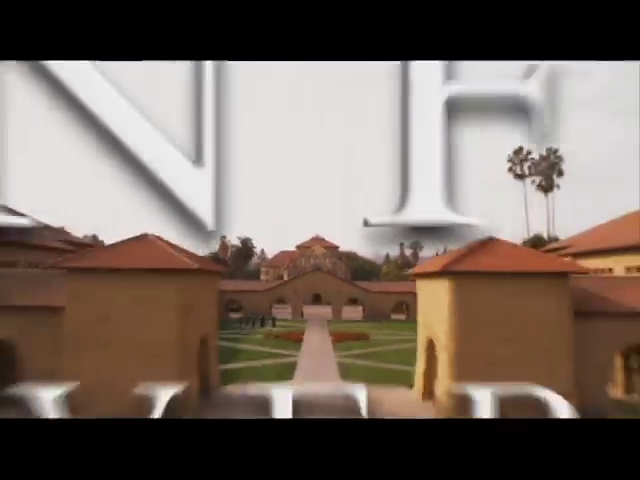
\includegraphics[width=0.78\textwidth]{lecture_02_figure_01.png}
  \caption{나중에 연속체 극한을 취할 때 사용할 유한 차분과 리만 합의 규칙.}
  \lectureframe{00:04:20}
  \label{fig:l02-calculus-board}
\end{figure}

이들은 미적분에서 익히 아는 정의다. 여기서 중요한 것은 스케일링이다. \(\Delta x_i\)는 \(\Delta\sigma\)의 한 거듭제곱을 곱하고, 합은 적분으로 바뀔 때 역거듭제곱을 하나 곱한다.

\subsection{디리클레 및 노이만 경계 조건}

유한 구간에서 푸리에 해석을 하려면 먼저 양 끝에서 어떤 조건을 둘지 정해야 한다. 여기서 반복해서 사용할 조건은 두 가지다.

\begin{align}
  \text{Dirichlet:}\qquad
  &x(0)=x(\pi)=0,
  \label{eq:l02-dirichlet}\\
  \text{Neumann:}\qquad
  &\left.\partial_\sigma x\right|_{\sigma=0}
   =
   \left.\partial_\sigma x\right|_{\sigma=\pi}
   =0.
  \label{eq:l02-neumann}
\end{align}

양끝을 고정한 바이올린 줄은 디리클레 그림을 보여 준다. 경계에서 변위는 영이다. 노이만 함수는 경계에서 영일 필요가 없으며, 각 경계에서 기울기가 영이다. 두 가지 특징적인 모양을 칠판에서 함께 볼 수 있다.

\begin{figure}[H]
  \centering
  \begin{minipage}[t]{0.48\textwidth}
    \centering
    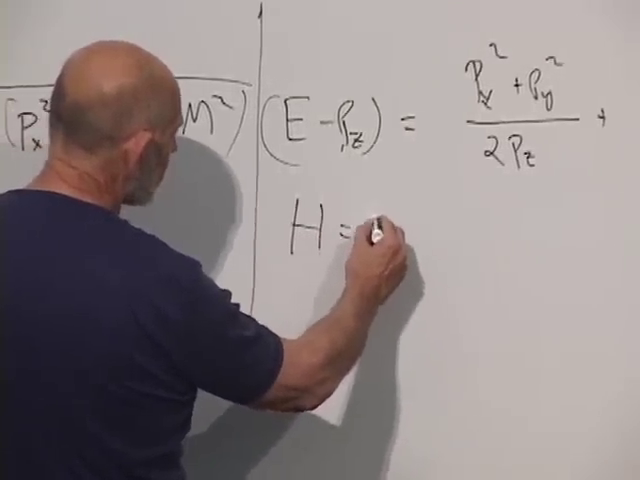
\includegraphics[width=\textwidth]{lecture_02_figure_02.png}
    \par\smallskip\footnotesize (a) 고정된 끝점과 기울기가 영인 끝점의 모양.
  \end{minipage}\hfill
  \begin{minipage}[t]{0.48\textwidth}
    \centering
    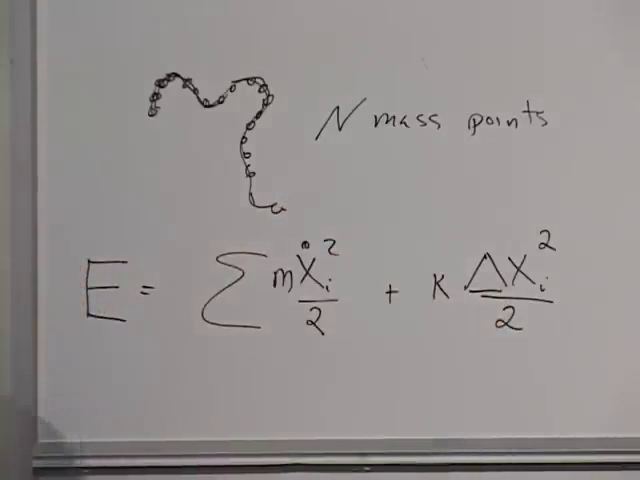
\includegraphics[width=\textwidth]{lecture_02_figure_03.png}
    \par\smallskip\footnotesize (b) 수직 막대를 따라 미끄러지는 가벼운 고리.
  \end{minipage}
  \caption{모양과 역학으로 나타낸 경계 조건. 고리가 미끄러지는 구조를 이용하면 자유 끝점의 횡방향 운동을 명확히 정의할 수 있다.}
  \lectureframe{00:08:50 and 00:12:15}
  \label{fig:l02-boundaries-board}
\end{figure}

\begin{figure}[H]
  \centering
  \begin{adjustbox}{max width=\linewidth}
  \begin{tikzpicture}[>=Latex,thick,scale=0.92]
    \begin{scope}
      \draw[->] (0,0) -- (4.4,0) node[right] {\(\sigma\)};
      \draw[->] (0,-1.25) -- (0,1.35) node[above] {\(x\)};
      \draw[blue!70!black]
        (0,0) .. controls (0.8,1.1) and (1.4,1.0) .. (2.0,0)
        .. controls (2.7,-1.0) and (3.4,-0.8) .. (4.1,0);
      \fill (0,0) circle (0.06);
      \fill (4.1,0) circle (0.06);
      \node at (2.05,-1.65) {Dirichlet: \(x=0\)};
    \end{scope}
    \begin{scope}[xshift=5.8cm]
      \draw[->] (0,0) -- (4.4,0) node[right] {\(\sigma\)};
      \draw[->] (0,-1.25) -- (0,1.35) node[above] {\(x\)};
      \draw[orange!85!black]
        (0,0.65) .. controls (0.8,0.65) and (1.1,-0.9) .. (2.0,-0.9)
        .. controls (2.9,-0.9) and (3.2,0.55) .. (4.1,0.55);
      \draw[orange!85!black] (0,0.65) -- (0.45,0.65);
      \draw[orange!85!black] (3.65,0.55) -- (4.1,0.55);
      \node at (2.05,-1.65) {Neumann: \(\partial_\sigma x=0\)};
    \end{scope}
  \end{tikzpicture}
  \end{adjustbox}
  \caption{디리클레 조건에서는 함수값이 고정되고, 노이만 조건에서는 기울기가 고정된다.}
  \label{fig:l02-boundaries-redraw}
\end{figure}

\begin{classroomqa}
\audiencequestion{열린 관이나 닫힌 관이 이 경계 조건 가운데 하나를 잘 보여 주는 예가 될까요?\lecturetimestamp{00:09:19}}
\lecturerresponse{그럴 수 있지만, 먼저 어떤 음향 변수를 전개하는지 밝혀야 한다. 압력 섭동과 종방향 변위는 열린 끝에서 서로 보완적인 이상화 조건을 따른다. 이 곁가지 질문을 칠판에서 결론내리기보다는 미끄럼 고리 모형을 사용하자. 질량이 거의 없는 고리는 막대를 따라 수직으로 움직일 수 있으므로, 끈의 끝은 자유롭고 노이만 조건이 직접 적용된다.}
\end{classroomqa}

\begin{classroomqa}
\audiencequestion{그래프가 수직으로 솟거나 날카로운 불연속을 가질 수 있나요?\lecturetimestamp{00:09:53}}
\lecturerresponse{푸리에 해석에서는 조각별 연속 함수에 고립된 불연속이 있어도 된다. 물리적인 끈에는 더 엄격한 조건이 필요하다. 불연속이 있으면 이웃한 점들이 끊어지고, 아래에서 유도할 연속체 에너지에서 공간 미분 \(\partial_\sigma x\)이 특이해진다. 따라서 함수 모양은 연속이고 미분 가능하다고 제한한다.}
\end{classroomqa}

\begin{classroomqa}
\audiencequestion{관의 열린 끝이나 다른 자유 끝점에도 왜 경계 조건이 있어야 하나요?\lecturetimestamp{00:11:14}}
\lecturerresponse{음향학의 예는 어떤 장을 택하느냐에 따라 달라지므로 토론에서 결론을 내리지 않았다. 역학의 예는 그렇지 않다. 매우 가벼운 고리는 자유롭게 미끄러질 수 있지만 줄의 마지막 구간에 연결되어 있다. 경계 조건을 가정하는 대신 뉴턴 법칙에서 유도하겠다. 끝점의 가속도가 유한하려면 기울기가 영이어야 한다.}
\end{classroomqa}

\subsection{푸리에 기저}

끝점의 조건을 정하면 그에 맞는 푸리에 기저도 정해진다. \(0\leq\sigma\leq\pi\)에서

\begin{align}
  x_D(\sigma)
  &=
  \sum_{n=1}^{\infty}x_n\sin(n\sigma),
  \label{eq:l02-dirichlet-series}\\
  x_N(\sigma)
  &=
  \sum_{n=0}^{\infty}x_n\cos(n\sigma).
  \label{eq:l02-neumann-series}
\end{align}

\eqref{eq:l02-dirichlet-series}의 모든 사인 함수는 양 끝점에서 0이 된다. \eqref{eq:l02-neumann-series}의 모든 코사인 함수는 끝점에서 미분값이 0이다. 하한이 서로 다른 데에는 이유가 있다. \(\sin(0\sigma)=0\)은 기여하지 않는 반면, \(\cos(0\sigma)=1\)는 상수 모드, 즉 영 모드다. 이 모드는 노이만 함수의 평균값을 나타낸다.

\begin{figure}[H]
  \centering
  \begin{minipage}[t]{0.48\textwidth}
    \centering
    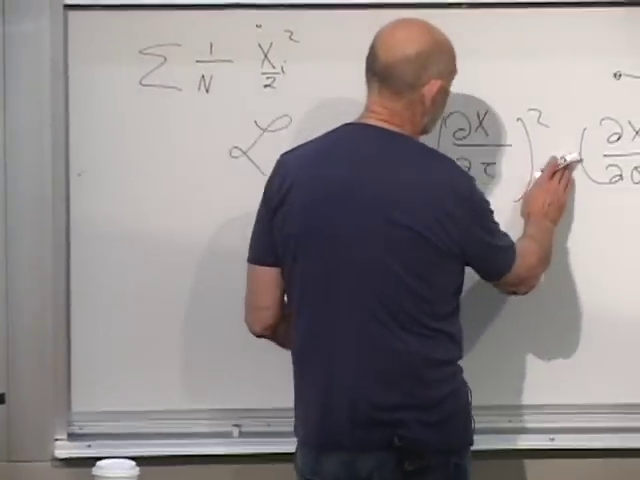
\includegraphics[width=\textwidth]{lecture_02_figure_04.png}
    \par\smallskip\footnotesize (a) 사인 및 코사인 전개.
  \end{minipage}\hfill
  \begin{minipage}[t]{0.48\textwidth}
    \centering
    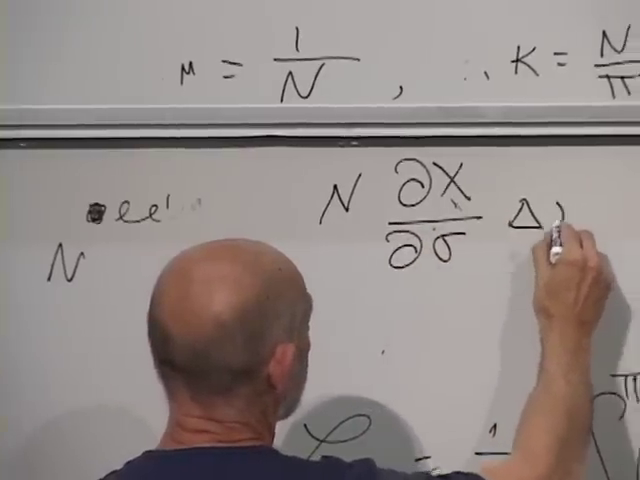
\includegraphics[width=\textwidth]{lecture_02_figure_05.png}
    \par\smallskip\footnotesize (b) 직교성과 예외적인 상수 모드.
  \end{minipage}
  \caption{줄의 모드를 대각화할 때 뒤에서 사용할 푸리에 성질.}
  \lectureframe{00:16:15 and 00:20:30}
  \label{fig:l02-fourier-board}
\end{figure}

미분하면 두 종류가 서로 바뀐다.

\begin{equation}
  \begin{aligned}
    \partial_\sigma\sin(n\sigma)&=n\cos(n\sigma),\\
    \partial_\sigma\cos(n\sigma)&=-n\sin(n\sigma).
  \end{aligned}
  \label{eq:l02-basis-derivatives}
\end{equation}

따라서 디리클레 급수를 미분하면 노이만 조건을 따르고, 노이만 급수를 미분하면 디리클레 조건을 따른다. 직교성 덕분에 서로 다른 모드 사이의 교차항은 사라진다.

\begin{align}
  \int_0^\pi\cos(n\sigma)\cos(m\sigma)\,d\sigma
  &=
  \frac{\pi}{2}\delta_{nm},
  && n,m\geq1,
  \label{eq:l02-cos-orthogonality}\\
  \int_0^\pi\sin(n\sigma)\sin(m\sigma)\,d\sigma
  &=
  \frac{\pi}{2}\delta_{nm},
  && n,m\geq1,
  \label{eq:l02-sin-orthogonality}\\
  \int_0^\pi 1\,d\sigma&=\pi .
  \label{eq:l02-zero-norm}
\end{align}

마지막 줄은 예외적인 \(n=m=0\) 코사인 노름이다. 상수는 영이 아닌 조화 모드와 같은 방식으로 정규화되지 않으며, 이 두 배 인자가 끈의 질량 중심 모드와 내부 모드를 구분해 준다.

\subsection{기억해 둘 진동자 공식 하나}

좌표를 재조정하여 역학적 질량을 1로 두면, 훅 법칙을 따르는 진동자는 다음과 같다.

\begin{align}
  E_{\mathrm{osc}}
  &=
  \frac12\dot q^{\,2}
  +\frac12\omega^2q^2,
  \label{eq:l02-oscillator-energy}\\
  L_{\mathrm{osc}}
  &=
  \frac12\dot q^{\,2}
  -\frac12\omega^2q^2.
  \label{eq:l02-oscillator-lagrangian}
\end{align}

\begin{figure}[H]
  \centering
  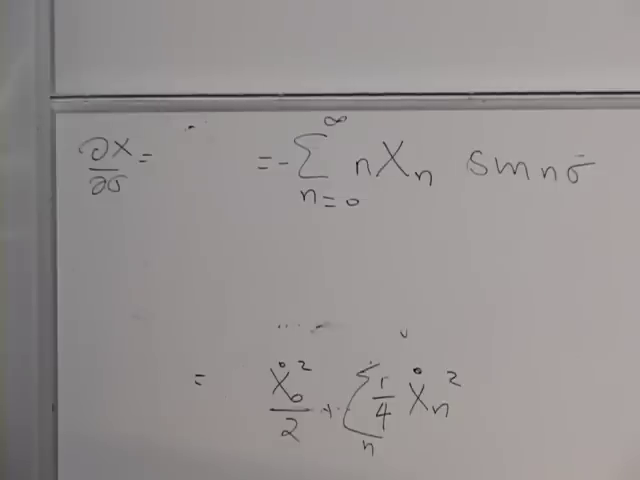
\includegraphics[width=0.68\textwidth]{lecture_02_figure_06.png}
  \caption{계수에서 \(q^2\)을 보면 \(\omega^2\)를 바로 알 수 있도록 쓴 진동자의 에너지.}
  \lectureframe{00:24:00}
  \label{fig:l02-oscillator-board}
\end{figure}

고전적으로는 \(\omega=\sqrt{\kappa/m}\)이다. 좌표를 재조정하여 \(m=1\)로 두었다. 양자역학에서는

\begin{equation}
  E_Q=\hbar\omega\left(Q+\frac12\right),
  \qquad Q=0,1,2,\ldots .
  \label{eq:l02-oscillator-spectrum}
\end{equation}

준위 간격만 볼 때는 모든 준위에 공통으로 들어가는 바닥 상태 항을 빼고, 각 양자가 \(\hbar\omega\)의 에너지를 갖는다고 말할 수 있다. 끈 계산도 처음에는 정확히 그렇게 하고, 전체 영점 에너지는 나중으로 미룬다.

\begin{classroomqa}
\audiencequestion{에너지 식에서 진동수는 어떻게 읽어 내나요?\lecturetimestamp{00:23:21}}
\lecturerresponse{재척도화하기 전에는 \(\omega=\sqrt{\kappa/m}\)이다. 단위질량으로 두면 퍼텐셜 항은 \(\frac12\omega^2q^2\)이므로, 이차항의 계수는 진동수의 제곱이다.}
\end{classroomqa}

\section{복합계가 입자가 되는 기준은 무엇인가?}

끈은 길게 뻗은 물체이며, 여러 조각이 서로 결합한 계로 모형화할 것이다. 그렇다면 그 양자 상태를 어떤 의미에서 입자라고 할 수 있을까? 점처럼 보이는지가 결정적인 기준일 수는 없다. 양성자와 중성자는 복합 입자다. 전자와 광자도 고유한 내부 구조가 확인된 적은 없지만 양자장의 드레싱을 동반한다. 아무것도 둘러싸지 않은 고전적 기하학적 점은 양자 들뜸을 그리는 적절한 그림이 아니다.

질량과 질량중심 위치만으로도 충분하지 않다. 밀폐된 기체 상자에도 둘 다 있다. 커피 잔에도 둘 다 있다. 보통 어느 쪽도 입자라고 부르지 않는다. 쪼갤 수 없어야 한다는 조건도 맞지 않는다. 양성자는 쪼갤 수 있고, 스핀 역시 미시적 입자와 거시적 물체를 구분해 주지 않는다.

유용한 기준은 스펙트럼상 고립되어 있는지 여부다. 수직축에 정지 에너지를 놓고 내부의 다른 상태에 도달하는 데 에너지가 얼마나 필요한지 살펴보자. 전자에는 그 바로 위에 실험적으로 접근할 수 있는 전자 들뜸 상태의 탑이 없다. 양성자에는 공명 상태가 있지만, 가장 낮은 상태에 도달하는 데 수백 MeV가 필요하다. 이는 양성자 질량의 상당 부분이다. 그 상태들은 서로 충분히 떨어져 있어 각각 식별할 수 있다.

커피 잔은 정반대다. 장파장 음향 모드에 임의로 작은 에너지를 더하거나, 분자를 살짝 흔들거나, 포논 하나를 만들 수 있다. 아주 좁은 에너지 구간에 어마어마하게 많은 상태가 빽빽이 들어 있다. 실험실 규모에서는 이들이 연속체를 이룬다. 이것이 입자와 \emph{잡다한 물질}을 실질적으로 구분하는 기준이다.

\begin{figure}[H]
  \centering
  \includegraphics[width=0.58\textwidth]{lecture_02_figure_07.png}
  \caption{보통 물질의 빽빽한 들뜸 상태와 고립된 입자 준위를 비교할 때 칠판에 그린 수직 에너지축.}
  \lectureframe{00:31:10}
  \label{fig:l02-spectrum-board}
\end{figure}

\begin{figure}[H]
  \centering
  \begin{adjustbox}{max width=\linewidth}
  \begin{tikzpicture}[>=Latex,thick]
    \begin{scope}
      \draw[->] (0,0) -- (0,4.8) node[above] {energy};
      \draw[blue!70!black,line width=1.2pt] (-1.0,0.65) -- (1.0,0.65);
      \draw[blue!70!black,line width=1.2pt] (-1.0,3.65) -- (1.0,3.65);
      \node[right] at (1.05,0.65) {ground state};
      \node[right] at (1.05,3.65) {first internal excitation};
      \draw[<->] (0.65,0.75) -- (0.65,3.55)
        node[midway,right] {large gap};
      \node at (0,-0.55) {particle-like};
    \end{scope}
    \begin{scope}[xshift=7.0cm]
      \draw[->] (0,0) -- (0,4.8) node[above] {energy};
      \foreach \y in {0.55,0.69,0.82,0.94,1.05,1.15,1.24,1.32,1.39,1.45,
        1.51,1.57,1.63,1.70,1.78,1.87,1.97,2.09,2.22,2.36,2.51,2.67,2.84,
        3.02,3.21,3.41,3.62,3.84,4.07}
        \draw[orange!85!black] (-0.95,\y) -- (0.95,\y);
      \node[right] at (1.05,2.25) {dense phonon and internal states};
      \node at (0,-0.55) {macroscopic matter};
    \end{scope}
  \end{tikzpicture}
  \end{adjustbox}
  \caption{강의에서 사용하는 조작적 입자 기준은 문자 그대로 점처럼 보이는지가 아니라 스펙트럼상 고립되어 있는지 여부다.}
  \label{fig:l02-particle-redraw}
\end{figure}

이 기준을 적용하면 철학적 질문을 계산 문제로 바꿀 수 있다. 끈을 양자화하고 내부 에너지 준위를 찾아 그 간격을 살펴보자. 끈의 첫 들뜸 상태가 플랑크 규모에 있고 관측되는 바닥 상태는 가볍다면, 그 간격은 현재 가속기가 도달하는 에너지보다 20자릿수 넘게 크다. 따라서 접근 가능한 모든 에너지 영역에서 끈은 기본 입자처럼 거동한다.

\begin{classroomqa}
\audiencequestion{입자처럼 보이는 성질은 관측 규모의 문제일 뿐인가요? 충분히 확대하면 준위들이 더 이상 분리되어 있지 않게 되나요?\lecturetimestamp{00:33:33}}
\lecturerresponse{확대하면 물체가 여러 구성 요소로 이루어져 있음을 알아낼 수 있지만, 스펙트럼이 사라지는 것은 아니다. 중요한 비교 대상은 실험의 에너지 분해능과 첫 내부 들뜸 상태까지의 간격이다. 그 간격이 엄청나게 크면 복합 물체도 계속 입자처럼 거동할 수 있다.}
\end{classroomqa}

\begin{classroomqa}
\audiencequestion{보통 바이올린 줄은 왜 입자가 아닌가요?\lecturetimestamp{00:34:37}}
\lecturerresponse{진동 양자 하나의 에너지는 거시적인 줄의 정지 에너지와 비교하면 측정할 수 없을 만큼 작다. 그러므로 아주 좁은 상대적 에너지 구간에도 양자 상태가 많이 들어간다. 이 줄은 스펙트럼 비교에서 고립된 쪽이 아니라 빽빽한 쪽에 속한다.}
\end{classroomqa}

\begin{classroomqa}
\audiencequestion{양자장이 가상 요동으로 둘러싸고 있어도 광자와 전자는 점입자인가요?\lecturetimestamp{00:35:40}}
\lecturerresponse{\emph{점}이라는 고전적 단어가 너무 많은 일을 떠맡고 있다. 물리적인 전자와 광자는 드레싱된 장의 들뜸 상태지만, 실험에서 어느 쪽도 고유한 구성 요소 구조나 유한한 형상 인자를 보인 적은 없다. 여기서 중요한 것은 둘 다 거의 축퇴된 내부 상태들이 빽빽이 이어지는 탑을 갖지 않는다는 점이다.\editorialnote{강의에서는 전자의 이상 자기 모멘트를 측정 가능한 양자적 퍼짐과 연결한다. 현대적 용어로 이상 자기 모멘트는 복사 드레싱 효과이지, 유한한 전자 반지름이 확인되었다는 증거가 아니다. 통상 점처럼 보인다는 말은 시험한 규모까지 고유한 내부 구조나 형상 인자가 검출되지 않았다는 뜻이다.}}
\end{classroomqa}

\begin{classroomqa}
\audiencequestion{광자의 크기는 진동수에 따라 달라지나요?\lecturetimestamp{00:36:49}}
\lecturerresponse{파장은 분명히 달라진다. 하지만 이는 고유한 구성 요소의 크기와는 다르다. 진동수를 바꾸면 파동 묶음과 파장이 달라질 뿐, 광자의 내부 반지름이 확인되는 것은 아니다.}
\end{classroomqa}

\section{큰 운동량에서의 정확한 횡방향 역학}

이제 상대론적 어려움으로 돌아가자. 빠르게 회전하는 곤봉은 질량중심을 정지시킨다고 해서 비상대론적으로 다룰 수 없다. 양 끝은 여전히 서로에 대해 상대론적으로 움직인다. 비상대론적 근사가 성립하지 않는 까닭은 내부의 상대 운동에 있다.

하지만 다른 극한이 있다. \(z\)축을 정하고, 계 전체를 아주 큰 양의 종방향 운동량 \(P_z\)을 갖도록 로런츠 변환한다. 횡방향 운동량은

\begin{equation}
  p_\perp^2=p_x^2+p_y^2
\end{equation}

유한하게 유지한다. 그러면 로런츠 변환 전의 내부 운동이 상대론적이었더라도 \(P_z\to\infty\) 극한에서 횡방향 투영은 정확히 비상대론적 해밀토니안 형태를 갖는다.

\begin{classroomqa}
\audiencequestion{무한 운동량은 질량을 가진 계가 실제로 빛의 속도에 도달한다는 뜻인가요?\lecturetimestamp{00:40:43}}
\lecturerresponse{유한한 로런츠 변환으로는 빛의 속도에 도달하지 못한다. \(P_z\)이 임의로 커질 때 잘 정의된 극한을 갖는 양들을 구성한다. 이 표현은 극한을 취하는 절차를 가리키며, \(v=c\)인 유한한 물리적 상태를 뜻하지 않는다.}
\end{classroomqa}

\begin{classroomqa}
\audiencequestion{어느 축을 택해야 하나요? 물체가 그 축을 중심으로 회전하거나 그 축을 가로질러 회전한다면 어떻게 되나요?\lecturetimestamp{00:41:14}}
\lecturerresponse{어느 축이든 택해도 되고, 계 전체를 그 축 방향으로 로런츠 변환하면 된다. 명시적으로 역학을 다루는 부분은 그 축에 수직인 평면으로의 투영이다. 회전하는 막대는 짧아져 보이거나 그 평면을 가로질러 쓸고 지나갈 수 있지만, 횡방향 투영은 비상대론적 형태를 갖는다.}
\end{classroomqa}

끈에는 이 표현을 특히 강력하게 만드는 성질이 하나 더 있다. 광전면 게이지에서는 종방향 내부 좌표가 독립적인 진동자가 아니다. 구속 조건에 따라 이 좌표들은 횡방향 운동으로부터 결정된다. 따라서 물리적 자유도를 복원하는 데 횡방향 끈만 알면 충분하다.

\begin{classroomqa}
\audiencequestion{독립적인 종방향 좌표가 없다는 말은 끈이 그저 얇은 샌드위치 안에 갇혀 있다는 뜻인가요?\lecturetimestamp{00:42:26}}
\lecturerresponse{로런츠 수축 때문에 로런츠 변환된 계에서 종방향 길이가 짧아지는 것은 맞지만, 그보다 더 강한 내용이다. 남아 있는 종방향 운동은 횡방향 운동에 의해 구속되므로 독립적으로 지정할 수 없다.}
\end{classroomqa}

\begin{classroomqa}
\audiencequestion{횡방향 자료로 줄이는 것이 홀로그래피 원리와 관련이 있나요?\lecturetimestamp{00:43:12}}
\lecturerresponse{홀로그래피 개념으로 이어진 사고의 흐름과 밀접하게 관련되어 있지만, 그 연결을 더 살펴보면 지금 계산에서 벗어나게 된다. 여기서는 횡방향 끈만 다루어도 된다는 점을 뒷받침하는 데에만 이 사실을 사용한다.}
\end{classroomqa}

\subsection{로런츠 변환 항을 빼고 시간을 재조정하기}

구성 입자의 질량, 운동 에너지, 결합 에너지를 모두 포함한 계 전체의 불변 질량을 \(M\)이라 하자. 단위 \(c=1\)에서는

\begin{equation}
  E=\sqrt{P_z^2+p_\perp^2+M^2}.
  \label{eq:l02-relativistic-energy}
\end{equation}

\(P_z\)이 \(p_\perp\)와 \(M\)보다 훨씬 크면

\begin{equation}
  E
  =
  P_z+\frac{p_\perp^2+M^2}{2P_z}
  +O(P_z^{-3}).
  \label{eq:l02-large-pz}
\end{equation}

\begin{figure}[H]
  \centering
  \includegraphics[width=0.76\textwidth]{lecture_02_figure_08.png}
  \caption{횡방향 운동량과 불변 질량을 유지한 채 전개한 큰 \(P_z\) 전개식.}
  \lectureframe{00:47:30}
  \label{fig:l02-large-pz-board}
\end{figure}

선도항은 크지만 내부 상태에 관한 정보는 담고 있지 않다. 부스트된 원자가 전체 종방향 운동량은 바꾸지 않은 채 내부 준위 사이에서 전이하는 경우처럼 \(P_z\)을 보존하는 과정에서는 이 항이 모든 에너지 차이에서 상쇄된다. 따라서 다음을 살펴보자.

\begin{equation}
  E-P_z=\frac{p_\perp^2+M^2}{2P_z}+O(P_z^{-3}).
  \label{eq:l02-residual-energy}
\end{equation}

분모에는 물리적 의미가 있다. 해밀토니안이 시간 변화를 생성하므로, 작은 잔류 에너지는 내부의 시간 변화가 실험실 시간으로는 느리게 보인다는 뜻이다. 이것이 시간 지연이다. 내부 운동을 유지하려면 재조정된 진화 매개변수 \(\tau\)를 도입하거나, 이와 동등하게 잔류 해밀토니안을 \(P_z\)배 한다.

\begin{equation}
  H_\perp
  \equiv
  \lim_{P_z\to\infty}P_z(E-P_z)
  =
  \frac12p_\perp^2+\frac12M^2.
  \label{eq:l02-transverse-hamiltonian}
\end{equation}

\begin{figure}[H]
  \centering
  \begin{minipage}[t]{0.48\textwidth}
    \centering
    \includegraphics[width=\textwidth]{lecture_02_figure_09.png}
    \par\smallskip\footnotesize (a) \(H=i\partial_t\)와 느려진 내부 시간 변화.
  \end{minipage}\hfill
  \begin{minipage}[t]{0.48\textwidth}
    \centering
    \includegraphics[width=\textwidth]{lecture_02_figure_10.png}
    \par\smallskip\footnotesize (b) 시간 재척도화 뒤의 유한한 횡방향 해밀토니안.
  \end{minipage}
  \caption{시간 지연된 잔여 에너지에서 유한한 2차원 해밀토니안으로.}
  \lectureframe{00:49:20 and 00:52:40}
  \label{fig:l02-lightfront-board}
\end{figure}

이는 2차원에서 움직이는 단위 질량 입자의 형태와 정확히 같다. 운동 에너지는 \(p_\perp^2/2\)이고 내부 에너지는 \(M^2/2\)이다. 특이한 점은 제곱이 들어간다는 것이다. 이 기술에서 정지 에너지 또는 결합 에너지의 역할을 하는 양은 불변 질량의 제곱에 비례한다.\editorialnote{통상적인 빛전면 변수 \(P^\pm=(E\pm P_z)/\sqrt2\)를 쓰면 정확한 질량 껍질 관계는 \(2P^+P^-=p_\perp^2+M^2\)이다. 식 \eqref{eq:l02-transverse-hamiltonian}은 같은 불변 관계를 강의에서 사용한 큰 \(P_z\) 정규화로 나타낸 것이다.}

\begin{classroomqa}
\audiencequestion{복합계의 각 부분이 가진 종방향 운동량은 어떻게 되었나요?\lecturetimestamp{00:51:30}}
\lecturerresponse{일반적인 복합 물체에서는 각 구성 요소가 전체 \(P_z\)의 어느 분율을 갖는지 유지해야 한다. 위 공식은 전체 질량중심 운동량을 사용한다. 끈 이론은 구속 조건에 따라 상대적 종방향 운동이 횡방향 자유도로부터 결정된다는 점에서 특별하다. 따라서 독립적인 종방향 진동자를 더할 필요가 없다.}
\end{classroomqa}

\section{이산적인 열린 끈}

이제 로런츠 변환된 끈은 횡방향 평면에서만 명시적으로 움직인다. 두 좌표를 \(X\)와 \(Y\)이라 하고, 우선 이를 \(N\)개의 질점과 \(N-1\)개의 용수철을 연결한 모형으로 근사하자. 각 점의 유사 질량이 \(\mu\)이고 이웃한 점 사이 용수철의 용수철 상수가 \(k\)라면 에너지는 다음과 같다.

\begin{equation}
  E_N
  =
  \sum_i
  \left[
    \frac{\mu}{2}
    \left(\dot X_i^2+\dot Y_i^2\right)
    +
    \frac{k}{2}
    \left((\Delta X_i)^2+(\Delta Y_i)^2\right)
  \right].
  \label{eq:l02-discrete-energy}
\end{equation}

모든 \(X\) 항에는 횡방향 평면이 두 방향을 가지므로 같은 형태의 \(Y\) 항이 있다. 첨자 \(i\)는 사슬을 따라 놓인 점을 가리키며, 공간 좌표가 아니다.

\begin{figure}[H]
  \centering
  \begin{minipage}[t]{0.48\textwidth}
    \centering
    \includegraphics[width=\textwidth]{lecture_02_figure_11.png}
    \par\smallskip\footnotesize (a) 구슬 사슬과 그 이산 에너지.
  \end{minipage}\hfill
  \begin{minipage}[t]{0.48\textwidth}
    \centering
    \includegraphics[width=\textwidth]{lecture_02_figure_12.png}
    \par\smallskip\footnotesize (b) \(N\)이 커질 때 \(\mu\)와 \(k\)의 스케일링.
  \end{minipage}
  \caption{연속체 극한을 취하기 전의 조절된 열린 줄.}
  \lectureframe{00:57:42 and 01:02:40}
  \label{fig:l02-chain-board}
\end{figure}

\begin{figure}[H]
  \centering
  \begin{adjustbox}{max width=\linewidth}
  \begin{tikzpicture}[>=Latex,thick]
    \foreach \i in {0,...,8} {
      \coordinate (p\i) at ({1.05*\i},{0.30*sin(55*\i)});
      \filldraw[white] (p\i) circle (0.10);
      \draw (p\i) circle (0.10);
    }
    \foreach \i in {0,...,7} {
      \pgfmathtruncatemacro{\j}{\i+1}
      \draw[decorate,decoration={zigzag,segment length=4pt,amplitude=2pt}]
        (p\i) -- (p\j);
    }
    \node[above=0.35cm of p0] {\(i=0\)};
    \node[above=0.35cm of p8] {\(i=N-1\)};
    \draw[<->] (0,-1.15) -- (8.4,-1.15)
      node[midway,below] {\(0\leq\sigma\leq\pi\)};
    \node at (4.2,1.25)
      {\(\mu=1/N,\quad k=N/\pi^2,\quad\Delta\sigma=\pi/N\)};
  \end{tikzpicture}
  \end{adjustbox}
  \caption{명확한 정규화 모형이다. 사슬을 더 잘게 나누면 점은 가벼워지고 미시적 용수철은 더 단단해진다.}
  \label{fig:l02-chain-redraw}
\end{figure}

매개변수 \(\sigma\)는 사슬을 따라 잰 위치를 나타낸다. \(0\leq\sigma\leq\pi\)로 두는 것은 관례일 뿐, 물리적 길이를 측정하는 것이 아니다. 이는 끈에 두 끝점이 있음을 상기시킨다. 나중에 닫힌 끈은 \(0\leq\sigma<2\pi\)에서 주기적으로 매개화할 것이다.

연속체 극한에서도 계 전체의 역학이 유한하게 유지되어야 한다. 구슬 하나의 질량을 고정하면 유사 총질량이 발산하므로 다음과 같이 둔다.

\begin{equation}
  \mu=\frac{1}{N}.
  \label{eq:l02-mu-scaling}
\end{equation}

그러면 \(N\mu=1\)이다. 이는 상대론적 정지 질량 \(M\)이 아니라 횡방향 유사 모형에서 관성 계수로 쓰이는 양이다.

용수철을 직렬로 연결하면 개수가 늘어날수록 전체가 더 부드러워진다. 사슬 전체의 강성을 유한하게 유지하려면 각 미시적 용수철은 더 단단해져야 한다.

\begin{equation}
  k=\frac{N}{\pi^2}
  =\frac{1}{\pi\,\Delta\sigma}.
  \label{eq:l02-k-scaling}
\end{equation}

필요한 조건은 \(k\propto N\)뿐이다. \(\pi^2\) 인자는 연속체 공식에 불필요한 \(\pi\) 인자가 남지 않도록 선택한 정규화다.

\begin{classroomqa}
\audiencequestion{\(\mu\)는 끈의 각 점이 갖는 물리적 정지 질량인가요?\lecturetimestamp{01:10:34}}
\lecturerresponse{아니다. 횡방향 사슬에 등장하는 비상대론적 유사 질량이다. 이를 \(M\)라고 부르면 상대론적 끈 상태 전체의 불변 정지 질량과 혼동하게 된다. 지금은 올바른 연속체 관성을 얻는 역할만 한다.}
\end{classroomqa}

\section{연속체 파동계}

처음에 마련한 규칙을 적용하자. \(1/N=\Delta\sigma/\pi\)이므로,

\begin{align}
  \sum_i\frac{\mu}{2}\dot X_i^2
  &=
  \frac{1}{2\pi}
  \sum_i\dot X_i^2\,\Delta\sigma
  \longrightarrow
  \frac{1}{2\pi}
  \int_0^\pi
  \left(\partial_\tau X\right)^2d\sigma ,
  \label{eq:l02-kinetic-limit}\\
  \sum_i\frac{k}{2}(\Delta X_i)^2
  &\longrightarrow
  \frac{1}{2\pi}
  \int_0^\pi
  \left(\partial_\sigma X\right)^2d\sigma .
  \label{eq:l02-potential-limit}
\end{align}

두 번째 줄에는 \(\Delta X_i=\partial_\sigma X\,\Delta\sigma\)과 \(k=1/(\pi\Delta\sigma)\)을 사용한다. \(Y\)에도 같은 계산이 적용된다.

\begin{figure}[H]
  \centering
  \begin{minipage}[t]{0.48\textwidth}
    \centering
    \includegraphics[width=\textwidth]{lecture_02_figure_13.png}
    \par\smallskip\footnotesize (a) 합을 적분으로, 차분을 도함수로 바꾸기.
  \end{minipage}\hfill
  \begin{minipage}[t]{0.48\textwidth}
    \centering
    \includegraphics[width=\textwidth]{lecture_02_figure_14.png}
    \par\smallskip\footnotesize (b) 완성된 연속체 에너지.
  \end{minipage}
  \caption{이산 사슬에서 \(\sigma\) 구간 위의 장으로.}
  \lectureframe{01:05:40 and 01:07:00}
  \label{fig:l02-continuum-board}
\end{figure}

그 결과 얻는 에너지와 라그랑지안은 다음과 같다.

\begin{align}
  E
  &=
  \frac{1}{2\pi}
  \int_0^\pi d\sigma\,
  \left[
    (\partial_\tau X)^2+(\partial_\tau Y)^2\right.\notag\\[-0.25em]
  &\hspace{6.5em}\left.
    +(\partial_\sigma X)^2+(\partial_\sigma Y)^2
  \right],
  \label{eq:l02-continuum-energy}\\
  L
  &=
  \frac{1}{2\pi}
  \int_0^\pi d\sigma\,
  \left[
    (\partial_\tau X)^2+(\partial_\tau Y)^2\right.\notag\\[-0.25em]
  &\hspace{6.5em}\left.
    -(\partial_\sigma X)^2-(\partial_\sigma Y)^2
  \right].
  \label{eq:l02-continuum-lagrangian}
\end{align}

\begin{figure}[H]
  \centering
  \includegraphics[width=0.78\textwidth]{lecture_02_figure_15.png}
  \caption{운동 항과 신축 항이 서로 반대 부호를 갖는 연속체 라그랑지안.}
  \lectureframe{01:08:48}
  \label{fig:l02-lagrangian-board}
\end{figure}

\(\sigma\)을 보통의 공간 좌표로, \(X\)를 장 \(\phi\)로 바꾸어 쓰면 이는 1차원 파동장의 에너지와 라그랑지안이다. \eqref{eq:l02-continuum-lagrangian}을 변분하면 다음을 얻는다.

\begin{equation}
  \left(\partial_\tau^2-\partial_\sigma^2\right)X=0,
  \qquad
  \left(\partial_\tau^2-\partial_\sigma^2\right)Y=0.
  \label{eq:l02-wave-equation}
\end{equation}

지금까지의 논증에서 이 방정식들을 직접 풀 필요는 없다. 파동이 끈을 따라 좌우로 이동하고 끝점에서 반사된다고 생각하면 된다. 디리클레 조건에서 반사되면 변위의 부호가 뒤집히고, 노이만 조건에서 반사되면 부호가 유지된다.

\begin{classroomqa}
\audiencequestion{\(\tau\)는 정확히 어떤 시간 변수인가요?\lecturetimestamp{01:08:54}}
\lecturerresponse{큰 \(P_z\) 기술에서 내부 운동을 추적하기 위해 사용하는 재조정된 시간이다. 계와 함께 로런츠 변환된 시계는 실험실 시간에 비해 느리게 간다. \(\tau\)는 이 시간 지연을 없애 내부 진동이 유한한 속도를 유지하도록 한다. 이 횡방향 역학에서는 단순히 시간으로 다룰 수 있다.\editorialnote{강의에서는 비격식적으로 \(\tau\)를 고유 시간이라고 부른다. 뻗어 있는 끈에서 정확한 광전면 진화 매개변수는 게이지를 고정해 재조정한 시간이지, 모든 점이 공유하는 하나의 불변 고유 시간은 아니다. 시간 지연에 관한 논증은 달라지지 않는다.}}
\end{classroomqa}

횡방향 평면에서 질량중심이 정지해 있을 때, \eqref{eq:l02-continuum-energy}의 내부 항은 \eqref{eq:l02-transverse-hamiltonian}의 정규화에 따라 \(M^2\)에 비례한다. 그래서 겉보기에는 평범한 이 파동계를 양자화하면 상대론적 질량 스펙트럼이 드러난다.

\begin{classroomqa}
\audiencequestion{\(P_z(E-P_z)\)에는 이름이 있나요?\lecturetimestamp{01:11:00}}
\lecturerresponse{보통 광원뿔 에너지 또는 광전면 에너지라고 부른다. 광전면이라는 이름이 진화면으로 사용하는 영공간을 더 잘 나타낸다. 전통적인 용어는 계산에 중요하지 않다.}
\end{classroomqa}

\begin{classroomqa}
\audiencequestion{여기서 말하는 원뿔은 보통 시공간의 광원뿔을 뜻하나요? 이 용어는 디랙이 도입했나요?\lecturetimestamp{01:11:17}}
\lecturerresponse{영좌표 구성은 45도 축으로 그릴 수 있지만, 여기서 진화면은 완전히 펼쳐지는 원뿔이 아니라 광전면이다. 디랙은 관련된 상대론적 동역학 형식들을 발전시켰다. 누가 역사적으로 이 이름을 붙였는지는 결론내리지 않았으며, 방정식에는 영향을 주지 않는다.}
\end{classroomqa}

\section{자유단이 노이만 조건을 따르는 이유}

이제 끝점 조건을 가정하지 않고 유도할 수 있다. 로런츠 변환된 횡방향 역학은 정확히 비상대론적 형태이므로 뉴턴 법칙을 적용해도 된다. 내부의 질점에는 양쪽 용수철이 힘을 가한다. 마지막 점에는 이웃한 점과 연결하는 용수철 하나만 힘을 가한다.

\begin{classroomqa}
\audiencequestion{상대론적 끈을 논하면서 어떻게 뉴턴 법칙을 사용할 수 있나요?\lecturetimestamp{01:14:52}}
\lecturerresponse{로런츠 변환하지 않은 시공간 운동 전체에 뉴턴 역학을 적용하는 것은 아니다. 무한 운동량 기술에서 횡방향 변수에 적용하는 것이다. 이 변수들의 해밀토니안은 정확히 비상대론적 형태를 갖는다.}
\end{classroomqa}

오른쪽 끝점에서 훅 법칙을 적용하면, 방향에 따른 부호를 제외하고 다음을 얻는다.

\begin{equation}
  F_{\mathrm{end}}
  =
  -k\,\Delta X
  =
  -\frac{1}{\pi\Delta\sigma}
   \left(\partial_\sigma X\,\Delta\sigma\right)
  =
  -\frac{1}{\pi}\partial_\sigma X .
  \label{eq:l02-endpoint-force}
\end{equation}

\begin{figure}[H]
  \centering
  \begin{minipage}[t]{0.48\textwidth}
    \centering
    \includegraphics[width=\textwidth]{lecture_02_figure_16.png}
    \par\smallskip\footnotesize (a) 국소 기울기에 비례하는 끝점 힘.
  \end{minipage}\hfill
  \begin{minipage}[t]{0.48\textwidth}
    \centering
    \includegraphics[width=\textwidth]{lecture_02_figure_17.png}
    \par\smallskip\footnotesize (b) 유한 가속도 조건.
  \end{minipage}
  \caption{자유 끝점 경계 조건을 뉴턴 법칙에서 유도하기.}
  \lectureframe{01:18:20 and 01:20:10}
  \label{fig:l02-neumann-board}
\end{figure}

마지막 점에 대한 뉴턴 방정식은 다음과 같다.

\begin{equation}
  \mu\,\partial_\tau^2X=F_{\mathrm{end}},
  \qquad
  \mu=\frac1N=\frac{\Delta\sigma}{\pi}.
  \label{eq:l02-endpoint-newton}
\end{equation}

\eqref{eq:l02-endpoint-force}과 \eqref{eq:l02-endpoint-newton}를 결합하면

\begin{equation}
  \partial_\sigma X
  =
  -\Delta\sigma\,\partial_\tau^2X
  \quad\text{at the right endpoint},
  \label{eq:l02-endpoint-scaling}
\end{equation}

왼쪽 끝점에서는 힘의 부호가 반대다. \(\partial_\sigma X\)이 영이 아닌 상수에 가까워지는 한편 \(\Delta\sigma\to0\)이면 끝점 가속도는 \(N\)에 비례해 발산한다. 따라서 가속도가 유한한 타당한 연속체 극한을 얻으려면 다음이 필요하다.

\begin{equation}
  \left.\partial_\sigma X\right|_{0,\pi}=0,
  \qquad
  \left.\partial_\sigma Y\right|_{0,\pi}=0.
  \label{eq:l02-open-neumann}
\end{equation}

\begin{figure}[H]
  \centering
  \begin{adjustbox}{max width=\linewidth}
  \begin{tikzpicture}[>=Latex,thick,scale=1.0]
    \coordinate (a) at (0,0);
    \coordinate (b) at (4.5,0.75);
    \filldraw[white] (a) circle (0.12);
    \draw (a) circle (0.12);
    \filldraw[white] (b) circle (0.12);
    \draw (b) circle (0.12);
    \draw[decorate,decoration={zigzag,segment length=6pt,amplitude=3pt}]
      (a) -- (b);
    \draw[dashed] (a) -- (0,-1.2);
    \draw[dashed] (b) -- (4.5,-1.2);
    \draw[<->] (4.85,0) -- (4.85,0.75)
      node[midway,right] {\(\Delta X\)};
    \draw[->,red!70!black] (b) -- (5.75,0.95)
      node[right] {\(F_{\rm end}=-k\Delta X\)};
    \node[below] at (0,-1.2) {\(N-1\)};
    \node[below] at (4.5,-1.2) {\(N\)};
    \node at (2.5,-2.0)
      {\(\mu\ddot X=-k\Delta X
      \ \Longrightarrow\
      \partial_\sigma X=-\Delta\sigma\,\ddot X\to0\)};
  \end{tikzpicture}
  \end{adjustbox}
  \caption{조절자 극한에서 마지막 점의 질량은 영으로 간다. 가속도가 유한하려면 끝점의 기울기가 영이어야 한다.}
  \label{fig:l02-neumann-redraw}
\end{figure}

양 끝점과 두 횡방향에 같은 논리를 적용하면 자유로운 열린 끈의 노이만 경계 조건을 얻는다.

\section{열린 끈의 정상 모드}

이제 라그랑지안과 경계 조건을 모두 갖춘 고전계가 완성되었다. 푸리에 해석을 거치면 양자화가 간단해진다. 끝점이 노이만 조건을 따르므로

\begin{align}
  X(\sigma,\tau)
  &=
  \sum_{n=0}^{\infty}X_n(\tau)\cos(n\sigma),
  \label{eq:l02-X-expansion}\\
  Y(\sigma,\tau)
  &=
  \sum_{n=0}^{\infty}Y_n(\tau)\cos(n\sigma).
  \label{eq:l02-Y-expansion}
\end{align}

코사인에는 \(\sigma\) 의존성이 모두 들어 있다. 계수에는 시간 의존성이 모두 들어 있다. \(X_n(\tau)\)와 \(Y_n(\tau)\)가 변하기 때문에 끈이 흔들린다.

\begin{figure}[H]
  \centering
  \includegraphics[width=0.78\textwidth]{lecture_02_figure_18.png}
  \caption{직교성 관계와 나란히 제시한 노이만 모드 전개. 이 관계를 이용하면 이중 합이 하나의 합으로 줄어든다.}
  \lectureframe{01:21:45}
  \label{fig:l02-mode-expansion-board}
\end{figure}

\subsection{운동에너지 항과 영 모드}

시간에 대해 미분하면

\begin{equation}
  \partial_\tau X
  =
  \sum_{n=0}^{\infty}\dot X_n(\tau)\cos(n\sigma).
  \label{eq:l02-time-mode}
\end{equation}

제곱하면 \(n\)와 \(m\)에 대한 이중 합이 생기지만,
\eqref{eq:l02-cos-orthogonality}에 따라 \(n\neq m\)인 항은 모두 사라진다.
상수 모드를 따로 다루면,

\begin{equation}
  \frac{1}{2\pi}\int_0^\pi
  (\partial_\tau X)^2\,d\sigma
  =
  \frac12\dot X_0^{\,2}
  +
  \frac14\sum_{n=1}^{\infty}\dot X_n^{\,2}.
  \label{eq:l02-mode-kinetic}
\end{equation}

\begin{figure}[H]
  \centering
  \includegraphics[width=0.76\textwidth]{lecture_02_figure_19.png}
  \caption{직교성 적분을 적용하면 운동에너지의 이중 합이 영 모드와 대각합으로 줄어든다.}
  \lectureframe{01:29:10}
  \label{fig:l02-mode-kinetic-board}
\end{figure}

상수 계수는 평균 위치이다.

\begin{equation}
  X_0(\tau)=\frac1\pi\int_0^\pi X(\sigma,\tau)\,d\sigma ,
  \label{eq:l02-center-of-mass}
\end{equation}

\(Y_0\)도 마찬가지다. 유사한 질량 밀도가 균일하다고 하면, 이 좌표들은 질량중심 좌표가 된다. 이 좌표에는 운동에너지가 있지만 복원력은 없다. 끈 전체가 횡방향 평면을 가로질러 자유롭게 움직일 수 있다.

\subsection{늘어남 항과 진동수}

공간에 대해 미분하면

\begin{equation}
  \partial_\sigma X
  =
  -\sum_{n=1}^{\infty}nX_n(\tau)\sin(n\sigma).
  \label{eq:l02-spatial-mode}
\end{equation}

균일한 병진 이동은 끈을 늘이지 않으므로 영 모드는 사라진다. 사인 함수의 직교성을 이용하면,

\begin{equation}
  \frac{1}{2\pi}\int_0^\pi
  (\partial_\sigma X)^2\,d\sigma
  =
  \frac14\sum_{n=1}^{\infty}n^2X_n^{\,2}.
  \label{eq:l02-mode-potential}
\end{equation}

\begin{figure}[H]
  \centering
  \includegraphics[width=0.76\textwidth]{lecture_02_figure_20.png}
  \caption{코사인 급수를 미분하면 사인 함수의 이중 합이 생기며, 직교성에 의해 다시 \(n=m\)이 성립한다.}
  \lectureframe{01:31:40}
  \label{fig:l02-mode-potential-board}
\end{figure}

따라서 \(X\)-부문의 라그랑지언은 다음과 같다.

\begin{equation}
  L_X
  =
  \frac12\dot X_0^{\,2}
  +
  \frac14\sum_{n=1}^{\infty}
  \left(
    \dot X_n^{\,2}-n^2X_n^{\,2}
  \right),
  \label{eq:l02-X-lagrangian}
\end{equation}

\(Y\)에도 같은 식이 성립한다. 이에 대응하는 에너지에서는 \(n^2X_n^2\) 앞에 양의 부호가 붙는다. 영이 아닌 각 모드는 서로 독립인 조화 진동자이며, \eqref{eq:l02-oscillator-lagrangian}와 비교하면 다음을 얻는다.

\begin{equation}
  \omega_n=n,
  \qquad n=1,2,3,\ldots .
  \label{eq:l02-mode-frequency}
\end{equation}

\begin{figure}[H]
  \centering
  \includegraphics[width=0.80\textwidth]{lecture_02_figure_21.png}
  \caption{분리된 진동자의 라그랑지언과 \(\omega_n=n\)라는 결론. 아래에는 이와 동일한 \(Y\) 모드 계열이 표시되어 있다.}
  \lectureframe{01:35:50}
  \label{fig:l02-oscillator-modes-board}
\end{figure}

정상 모드는 단순히 끈의 고조파들이다. 첫 번째 모드는 천천히 휘고, 두 번째 모드의 진동수는 그 두 배이며, 세 번째 모드는 세 배이다. 이런 식으로 계속된다. 자유 이론에서 한 고조파가 다른 고조파와 결합하지 않는 것은 직교성 덕분이다.

\begin{classroomqa}
\audiencequestion{\(n=0\) 진동자는 어떻게 되었나요?\lecturetimestamp{01:34:49}}
\lecturerresponse{진동수가 0인 까닭은 이것이 내부 진동자가 전혀 아니기 때문입니다. 이 모드는 질량중심을 병진 이동시킵니다. 끈 전체를 특정한 횡방향 위치로 되돌리는 용수철은 없으므로, 영 모드는 자유 입자의 좌표입니다.}
\end{classroomqa}

질량중심의 운동에너지 항을 빼면 내부 에너지가 남는다.

\begin{equation}
  E_{\mathrm{int}}
  =
  \frac14
  \sum_{n=1}^{\infty}
  \left[
    \dot X_n^{\,2}+n^2X_n^{\,2}
    +\dot Y_n^{\,2}+n^2Y_n^{\,2}
  \right].
  \label{eq:l02-internal-energy}
\end{equation}

라이트프런트 정규화에서 이 양은 끈 상태의 불변 질량 제곱에 비례한다. 이로써 상대론적 질량 문제를 두 개의 셀 수 있는 진동자 계열에 대한 양자역학 문제로 바꾸었다.

\section{양자화된 준위와 입자 거동}

\(a_n^\dagger\)가 진동수 \(n\)인 \(X\) 진동자에 양자 하나를 생성하고, \(b_n^\dagger\)는 \(Y\)에 대해 같은 역할을 한다고 하자. 강의에서는 연산자를 체계적으로 다루는 일을 뒤로 미루지만, 이 표기법을 쓰면 준위 수를 쉽게 셀 수 있다. 바닥 상태의 에너지 오프셋을 기준으로 하면,

\begin{equation}
  \begin{aligned}
    \Delta E_{\mathrm{int}}
    &=\sum_{n=1}^{\infty}n\left(Q_n^X+Q_n^Y\right),\\
    Q_n^X,Q_n^Y&\in\{0,1,2,\ldots\}.
  \end{aligned}
  \label{eq:l02-quantized-energy}
\end{equation}

여기서 \(\hbar=1\)이다. 정수 \(n\)은 어떤 진동자가 여기되었는지를 나타내고, \(Q_n\)는 그 진동자에 들어 있는 양자의 수를 센다.\editorialnote{각 진동자는 영점 에너지도 기여한다. 무한합을 계산하려면 정칙화가 필요하며, 이 합이 끈 질량 공식의 절편을 정한다. 여기서는 바닥 상태의 에너지 오프셋을 일부러 명시하지 않고 여기 준위만 센다.}

진동자 진공 \(\ket{0}\)은 빈 시공간이 아니다. 내부 진동자가 여기되지 않은 열린 끈 하나를 뜻한다. 이 상태에는 에너지와 운동량이 있으며, 끈 스펙트럼에서 차지하는 위치도 정해져 있다.

첫 번째 준위에는 두 상태가 있다.

\begin{equation}
  a_1^\dagger\ket{0},
  \qquad
  b_1^\dagger\ket{0},
  \label{eq:l02-level-one}
\end{equation}

이는 가장 낮은 고조파의 편극이 \(X\) 방향이거나 \(Y\) 방향인 경우에 해당한다. 이들의 선형 결합으로 임의의 횡방향 편극을 나타낼 수 있다.

두 번째 준위에는 다섯 상태가 있다.

\begin{equation}
  (a_1^\dagger)^2\ket{0},
  \quad
  a_1^\dagger b_1^\dagger\ket{0},
  \quad
  (b_1^\dagger)^2\ket{0},
  \quad
  a_2^\dagger\ket{0},
  \quad
  b_2^\dagger\ket{0}.
  \label{eq:l02-level-two}
\end{equation}

그중 세 상태는 첫 번째 고조파의 양자 두 개를 사용하고, 두 상태는 두 번째 고조파의 양자 하나를 사용한다. 두 구성 모두 준위 단위 두 개에 해당하는 에너지가 든다.

\begin{figure}[H]
  \centering
  \includegraphics[width=0.76\textwidth]{lecture_02_figure_22.png}
  \caption{청중의 질문을 받은 뒤 다시 세어 보는 두 번째 준위의 다섯 상태. 두 개의 이중 여기 상태, 하나의 혼합 여기 상태, 두 개의 두 번째 고조파 여기 상태로 이루어진다.}
  \lectureframe{01:44:00}
  \label{fig:l02-levels-board}
\end{figure}

\begin{figure}[H]
  \centering
  \begin{adjustbox}{max width=\linewidth}
  \begin{tikzpicture}[>=Latex,thick]
    \draw[->] (0,0) -- (0,5.1) node[above] {\(\Delta E_{\rm int}\)};
    \draw[blue!70!black] (-0.65,0.55) -- (0.65,0.55);
    \node[right] at (0.85,0.55) {\(\ket{0}\) \quad multiplicity \(1\)};
    \draw[blue!70!black] (-0.65,2.15) -- (0.65,2.15);
    \node[right] at (0.85,2.15)
      {\(a_1^\dagger\ket{0},\ b_1^\dagger\ket{0}\)
      \quad multiplicity \(2\)};
    \draw[blue!70!black] (-0.65,3.75) -- (0.65,3.75);
    \node[right,text width=8.6cm] at (0.85,3.75)
      {\((a_1^\dagger)^2\ket{0},
      a_1^\dagger b_1^\dagger\ket{0},
      (b_1^\dagger)^2\ket{0},
      a_2^\dagger\ket{0},\ b_2^\dagger\ket{0}\)
      \quad multiplicity \(5\)};
    \node[left] at (-0.75,0.55) {\(0\)};
    \node[left] at (-0.75,2.15) {\(1\)};
    \node[left] at (-0.75,3.75) {\(2\)};
  \end{tikzpicture}
  \end{adjustbox}
  \caption{횡방향이 두 개인 열린 끈의 처음 세 여기 준위.}
  \label{fig:l02-levels-redraw}
\end{figure}

\begin{classroomqa}
\audiencequestion{두 번째 여기 준위의 상태는 네 개인가요, 다섯 개인가요?\lecturetimestamp{01:43:04}}
\lecturerresponse{다섯 개입니다. \(X_1\)를 두 번 여기하는 경우, \(Y_1\)를 두 번 여기하는 경우, 그리고 둘을 각각 한 번씩 여기하는 경우가 세 상태입니다. \(X_2\)를 한 번 여기하는 경우와 \(Y_2\)를 한 번 여기하는 경우가 두 상태를 더합니다. 다음 두 준위의 상태 수를 세어 보는 것이 제안된 연습 문제입니다.}
\end{classroomqa}

핵심 결론은 이미 분명하다. 연속된 준위 사이에는 유한한 간격이 있고, 각 준위의 축퇴도 유한하다. 따라서 양자화된 끈은 커피나 기체, 보통 바이올린 현과 구별되는 스펙트럼 기준에서 입자와 같은 성질을 갖는다. 이후에는 어떤 상태가 물리적으로 허용되는지, 또 어떤 병리적 상태를 제거해야 하는지 살펴볼 것이다.

\section{열린 끈의 상호작용이 닫힌 끈을 만드는 이유}

열린 끈에는 양 끝점이 있다. 끈의 기본적인 상호작용은 끈을 합치거나 나누는 것이다. 강입자 모형에서는 한쪽 끝에 쿼크가, 다른 쪽 끝에 반쿼크가 있다고 생각할 수 있다. 이들이 소멸하면 두 끈 조각이 합쳐진다. 여기서 나중에 다룰 기본 끈이 반드시 이런 문자 그대로의 강입자 끝점 해석을 따라야 하는 것은 아니지만, 국소적인 결합 규칙은 여전히 성립한다.

이제 열린 끈 하나가 요동하여 양 끝점이 서로 가까워진다고 하자. 국소적으로 끝점은 다른 끝점이 다른 끈에 속하는지 자기 끈에 속하는지 알 수 없다. 끝점끼리 결합할 수 있다면, 여기서도 결합하여 닫힌 고리를 만들 수 있다.

\begin{figure}[H]
  \centering
  \includegraphics[width=0.70\textwidth]{lecture_02_figure_23.png}
  \caption{열린 끈이 요동하여 두 끝점이 만나 닫힌 고리를 이루는 모습을 칠판에 그린 그림.}
  \lectureframe{01:47:00}
  \label{fig:l02-closed-board}
\end{figure}

\begin{figure}[H]
  \centering
  \begin{adjustbox}{max width=\linewidth}
  \begin{tikzpicture}[>=Latex,thick]
    \begin{scope}
      \draw[blue!70!black]
        (0,0) .. controls (0.8,1.2) and (1.7,-1.0) .. (2.6,0.45)
        .. controls (3.4,1.55) and (4.0,0.3) .. (4.7,0.85);
      \fill (0,0) circle (0.09);
      \fill (4.7,0.85) circle (0.09);
      \node at (2.35,-1.25) {open string fluctuation};
    \end{scope}
    \draw[->,line width=1pt] (5.25,0.3) -- (6.65,0.3)
      node[midway,above] {join};
    \begin{scope}[xshift=8.1cm]
      \draw[orange!85!black]
        (0,0) .. controls (0.3,1.5) and (2.5,1.8) .. (3.1,0.3)
        .. controls (3.5,-1.1) and (0.7,-1.5) .. (0,0);
      \node at (1.55,-1.85) {closed string};
    \end{scope}
  \end{tikzpicture}
  \end{adjustbox}
  \caption{끝점 결합이 허용되면 열린 끈은 자기 자신과 결합해 닫힌 끈이 될 수 있다.}
  \label{fig:l02-closed-redraw}
\end{figure}

따라서 닫힌 끈은 열린 끈 없이도 이론에 포함될 수 있지만, 열린 끈이 있는 상호작용 이론에서는 닫힌 끈을 일관되게 배제할 수 없다. 이 비대칭성이 중요한 예측이다. 스펙트럼에 대한 구체적인 해석은 뒤에서 다루겠지만, 도달할 결론은 이미 보인다. 질량이 없는 열린 끈 상태는 흔히 광자와 같은 게이지 입자를 제공하고, 닫힌 끈 스펙트럼에는 질량이 없는 스핀 2 상태인 중력자가 들어 있다. 끈 이론에 상호작용이 있으면 닫힌 끈, 따라서 중력은 선택적으로 덧붙이는 요소가 아니다.

\chapter{열린 끈의 양자에서 타키온과 중력까지}

\lectureoverview{이제 지난 강의에서 구한 정상 모드를 양자화하고, 그 결과 어떤 입자 상태가 만들어지는지 살펴보자. 각 횡방향 모드는 조화 진동자이지만, 정규화 방식은 다소 낯설다. \(n\) 모드를 들뜨게 하면 광전면 에너지가, 따라서 질량제곱 준위가 \(n\)만큼 증가한다. 열린 끈의 첫 번째 들뜬 준위는 질량이 없는 벡터의 두 횡방향 편광과 정확히 같은 방식으로 변환한다. 그러므로 상대론적 일관성을 만족하려면 바닥 상태의 질량제곱은 음수여야 한다. 이 상태가 보손 끈의 타키온이다. 타키온의 실제 의미는 현실적으로 빛보다 빠르게 움직이는 입자가 아니라 불안정한 진공이다. 마지막으로 끈이 상호작용하면 끈의 결합과 분리 때문에 닫힌 끈을 피할 수 없으며, 닫힌 끈의 가장 낮은 들뜸은 중력자가 된다.}

\section{각 끈 모드에 숨어 있는 진동자}

횡방향 좌표 \(X\) 하나에 대해, \(n\)번째 비영 정상 모드의 에너지와 라그랑지안은

\begin{align}
  E_n
  &=
  \frac14\dot X_n^{\,2}
  +\frac{n^2}{4}X_n^2,
  \label{eq:l03-mode-energy}\\
  L_n
  &=
  \frac14\dot X_n^{\,2}
  -\frac{n^2}{4}X_n^2.
  \label{eq:l03-mode-lagrangian}
\end{align}

\(1/4\) 인자는 오류가 아니다. 끈의 작용을 독립적인 푸리에 모드로 환원할 때 선택한 정규화가 이 인자에 반영되어 있다. 따라서 해밀토니안을 구성하는 첫 단계는 정준 운동량을 계산하는 것이다.

\begin{equation}
  p_n=\frac{\partial L_n}{\partial\dot X_n}
     =\frac12\dot X_n,
  \qquad
  \dot X_n=2p_n.
  \label{eq:l03-canonical-momentum}
\end{equation}

르장드르 변환을 하면 다음을 얻는다.

\begin{equation}
  H_n=p_n\dot X_n-L_n
     =p_n^2+\frac{n^2}{4}X_n^2.
  \label{eq:l03-mode-hamiltonian}
\end{equation}

\begin{figure}[H]\centering
  \includegraphics[width=0.82\textwidth]{lecture_03_figure_01.png}\caption{열린 끈에서 물려받은 정규화로 나타낸 모드의 에너지, 라그랑지안, 정준 운동량, 해밀토니안.}\lectureframe{00:05:40}\label{fig:l03-mode-hamiltonian-board}\end{figure}

\(H_n\)을 인수분해하려면 \(X_n\)와 \(p_n\)를 다음과 같이 결합한다.

\begin{equation}
  \frac{nX_n}{2}\pm i p_n.
\end{equation}

고전적으로는 두 인자가 교환하겠지만, 양자역학에서는 다음과 같다.

\begin{equation}
  [X_n,p_m]=i\delta_{nm}
  \label{eq:l03-canonical-commutator}
\end{equation}

\(\hbar=1\)인 단위를 사용하면 다음과 같다. 교차항들은 상쇄되어 사라지는 것이 아니다. 고정된 모드에 대해

\begin{align}
  \left[\frac{nX_n}{2}+ip_n,
        \frac{nX_n}{2}-ip_n\right]
  &=n,
  \label{eq:l03-unscaled-commutator}\\
  \left(\frac{nX_n}{2}-ip_n\right)
  \left(\frac{nX_n}{2}+ip_n\right)
  &=H_n-\frac n2.
  \label{eq:l03-factorized-hamiltonian}
\end{align}

\begin{figure}[H]\centering
  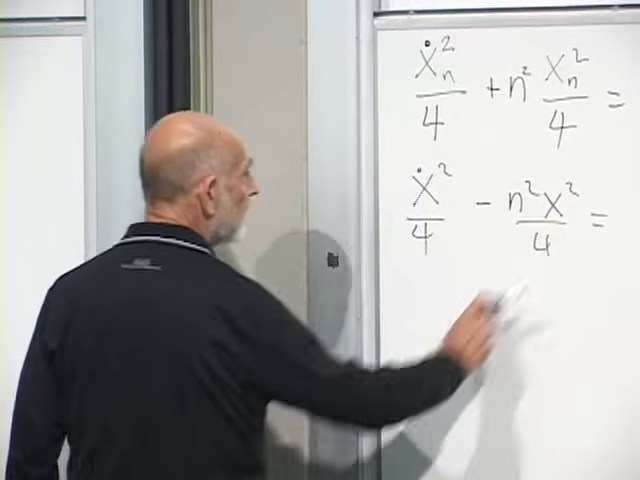
\includegraphics[width=0.82\textwidth]{lecture_03_figure_02.png}\caption{정준 교환자가 \(n\) 인자를 만들어 내는 과정을 칠판에서 계산한 모습.}\lectureframe{00:10:30}\label{fig:l03-commutator-board}\end{figure}

\(n\) 인자는 사다리 연산자를 어떻게 정규화해야 하는지 알려 준다.

\begin{align}
  a_n
  &\equiv
  \frac{\sqrt n}{2}X_n+\frac{i}{\sqrt n}p_n,
  \label{eq:l03-annihilator}\\
  a_n^\dagger
  &\equiv
  \frac{\sqrt n}{2}X_n-\frac{i}{\sqrt n}p_n.
  \label{eq:l03-creator}
\end{align}

이 연산자들은 다음 관계를 만족한다.

\begin{equation}
  [a_n,a_m^\dagger]=\delta_{nm},
  \qquad
  H_n=n\left(a_n^\dagger a_n+\frac12\right).
  \label{eq:l03-oscillator-algebra}
\end{equation}

따라서 \(a_n^\dagger\)는 \(n\)번째 진동자에 양자 하나를 더하지만, 그 양자는 모드 에너지를 \(n\)만큼 가진다. 익숙한 진동자의 에너지 간격이 사라진 것은 아니다. 그 진동수는 \(\omega_n=n\)이다.

\begin{figure}[H]\centering
  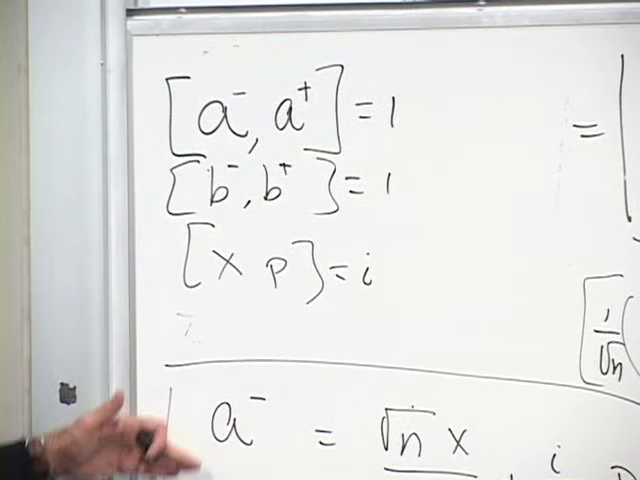
\includegraphics[width=0.82\textwidth]{lecture_03_figure_03.png}\caption{\(n\)번째 끈 진동자의 정규화된 소멸 연산자와 생성 연산자.}\lectureframe{00:12:00}\label{fig:l03-ladder-board}\end{figure}

\subsection{두 개의 횡방향 모드 계열}

시공간이 4차원일 때, \(z\)축을 따라 매우 큰 운동량을 가진 끈에는 횡방향 좌표가 두 개, \(X\)와 \(Y\)가 있다. 따라서 서로 독립적인 진동자 계열 두 개가 필요하다. \(a_n,a_n^\dagger\)는 \(X\) 모드에 작용하고, \(b_n,b_n^\dagger\)는 \(Y\) 모드에 작용한다고 하자. 좌표에 대해 \eqref{eq:l03-annihilator}--\eqref{eq:l03-creator}를 풀면 다음을 얻는다.

\begin{equation}
  X_n=\frac{a_n+a_n^\dagger}{\sqrt n},
  \qquad
  Y_n=\frac{b_n+b_n^\dagger}{\sqrt n}.
  \label{eq:l03-mode-coordinates}
\end{equation}

\begin{figure}[H]\centering
  \includegraphics[width=0.78\textwidth]{lecture_03_figure_04.png}\caption{생성 연산자와 소멸 연산자로 모드 좌표를 구하는 과정.}\lectureframe{00:17:05}\label{fig:l03-coordinate-operator-board}\end{figure}

열린 끈의 좌표는 노이만 모드로 전개했다.

\begin{align}
  X(\sigma,\tau)
  &=X_{\rm cm}(\tau)
    +\sum_{n=1}^{\infty}X_n(\tau)\cos(n\sigma),
  \label{eq:l03-X-fourier}\\
  Y(\sigma,\tau)
  &=Y_{\rm cm}(\tau)
    +\sum_{n=1}^{\infty}Y_n(\tau)\cos(n\sigma).
  \label{eq:l03-Y-fourier}
\end{align}

끝점에서 기울기가 사라지므로 코사인 함수가 나타난다. \eqref{eq:l03-mode-coordinates}을 대입하면 끈 자체가 연산자가 된다:

\begin{align}
  X(\sigma,\tau)
  &=X_{\rm cm}(\tau)
    +\sum_{n=1}^{\infty}
      \frac{a_n(\tau)+a_n^\dagger(\tau)}{\sqrt n}
      \cos(n\sigma),
  \label{eq:l03-X-operator}\\
  Y(\sigma,\tau)
  &=Y_{\rm cm}(\tau)
    +\sum_{n=1}^{\infty}
      \frac{b_n(\tau)+b_n^\dagger(\tau)}{\sqrt n}
      \cos(n\sigma).
  \label{eq:l03-Y-operator}
\end{align}

\begin{figure}[H]\centering
  \begin{minipage}[t]{0.48\textwidth}\centering
    \includegraphics[width=\textwidth]{lecture_03_figure_05.png}\par\smallskip\footnotesize (a) 좌표의 모드 전개.\end{minipage}\hfill
  \begin{minipage}[t]{0.48\textwidth}\centering
    \includegraphics[width=\textwidth]{lecture_03_figure_06.png}\par\smallskip\footnotesize (b) 사다리 연산자를 끈 좌표에 대입한 모습.\end{minipage}\caption{양자 열린 끈의 형태는 모든 횡방향 진동자 연산자를 모아 구성된다.}\lectureframe{00:20:35 and 00:21:05}\label{fig:l03-string-coordinate-board}\end{figure}

\begin{classroomqa}\audiencequestion{\(X_n\)도 \(\sigma\)의 함수인가?\lecturetimestamp{00:21:48}}\lecturerresponse{아니다. \(\sigma\) 의존성은 전적으로 \(\cos(n\sigma)\)에 들어 있다. 계수 \(X_n\)는 그 공간적 패턴의 시간 의존 진폭이므로, \(X_n=X_n(\tau)\)이다.}\end{classroomqa}

\begin{classroomqa}\audiencequestion{올림 연산자와 내림 연산자는 왜 부호가 거꾸로인 것처럼 보이나요?\lecturetimestamp{00:23:13}}\lecturerresponse{\(ip_n\)의 겉으로 드러나는 부호는 연산자 이름을 정하는 기준이 아니다. 해밀토니안과의 교환자를 계산하라. \([H_n,a_n^\dagger]=n a_n^\dagger\)을 만족하는 연산자는 에너지를 올리고, \([H_n,a_n]=-n a_n\)을 만족하는 연산자는 에너지를 내린다.}\end{classroomqa}

두 횡방향 모드 계열은 설명을 위한 4차원 그림이다. 일관되게 양자화된 보손 끈에는 시공간 차원이 26개 있으므로, 횡방향 진동자 계열은 두 개가 아니라 24개다. 아래의 논리는 달라지지 않는다. 첫 번째 준위의 상태 수는 같은 차원에서 질량이 없는 벡터의 물리적 편광 수와 일치해야 한다.

\section{질량 있는 입자의 스핀과 질량 없는 입자의 헬리시티}

끈 상태에 스핀을 부여하기 전에 한 가지를 분명히 구분해야 한다. 스핀 \(J\)인 질량 있는 입자에는 스핀 상태가 \(2J+1\)개 있다.

\begin{equation}
  m_J=-J,-J+1,\ldots,J-1,J.
  \label{eq:l03-massive-spin-multiplet}
\end{equation}

예를 들어 스핀 1인 질량 있는 입자에는 편광이 세 개 있고, 스핀 2인 질량 있는 입자에는 다섯 개 있다. 정지계로 가면 그 이유를 알 수 있다. 정지계에서는 모든 공간 회전이 가능하다. 스핀축을 회전시킨 다음 원래 계로 부스트하면, \(2J+1\)개의 성분이 모두 동일한 상대론적 입자에 속한다.

질량 없는 입자에는 정지계가 없다. 그 불변 스핀 표지는 헬리시티, 즉 운동 방향을 따른 각운동량이다. 광자에는 \(h=+1\)와 \(h=-1\)만 있고, 중력자에는 \(h=+2\)와 \(h=-2\)만 있다. 스칼라는 \(h=0\) 상태를 가진다. 이 강의에서는 반사 대칭을 이용해 두 헬리시티를 짝짓는다. 키랄 이론에서는 하나의 질량 없는 기약 표현이 헬리시티 하나만 가질 수 있으므로, 두 헬리시티의 짝짓기는 질량이 없다는 사실만으로 따라오는 결론이 아니라 추가적인 대칭에 관한 진술이다.\editorialnote{현대적인 작은 군 분류에서는 헬리시티 하나만 갖는 질량 없는 표현을 허용한다. 익숙한 광자와 중력자의 경우에는 패리티 또는 적절한 CPT 완비 장 내용이 반대 헬리시티를 제공한다.}

\begin{figure}[H]\centering
  \begin{minipage}[t]{0.45\textwidth}\centering
    \includegraphics[width=\textwidth]{lecture_03_figure_07.png}\par\smallskip\footnotesize (a) 칠판에서 시작한 스핀 상태 수 계산.\end{minipage}\hfill
  \begin{minipage}[t]{0.5\textwidth}\centering
    \begin{adjustbox}{max width=\linewidth}\begin{tabular}{@{}ccc@{}}\toprule
      스핀 & 질량 있는 상태 & 질량 없는 헬리시티 \\\midrule
      \(0\) & \(1\) & \(0\) \\\(1\) & \(3\) & \(+1,-1\) \\\(2\) & \(5\) & \(+2,-2\) \\\bottomrule
    \end{tabular}\end{adjustbox}\end{minipage}\caption{질량이 있으면 정지계가 없어지고, 그에 따라 중간 스핀 투영값도 사라진다.}\lectureframe{00:27:40}\label{fig:l03-spin-count}\end{figure}

\subsection{선편광과 원편광}

\(z\) 방향으로 진행하는 광자를 생각하자. 두 횡방향 선편광은 \(\ket{x}\)와 \(\ket{y}\)이다. 이들은 헬리시티 고유상태가 아니다. 원편광 상태는 다음과 같다.

\begin{align}
  \ket{R}
  &=\frac{1}{\sqrt2}\left(\ket{x}+i\ket{y}\right),
  \label{eq:l03-right-circular}\\
  \ket{L}
  &=\frac{1}{\sqrt2}\left(\ket{x}-i\ket{y}\right),
  \label{eq:l03-left-circular}
\end{align}

오른쪽과 왼쪽을 명명하는 관례에 따라 헬리시티가 \(+1\)와 \(-1\)인 두 상태가 있다. 선형 편광된 광자는 이 두 결과의 중첩이다. 평균 헬리시티는 영일 수 있지만, 헬리시티를 측정해도 스핀이 영인 광자가 나오는 일은 결코 없다. 마찬가지로,

\begin{equation}
  \frac{1}{\sqrt2}\left(\ket{x}+\ket{y}\right)
\end{equation}

는 단순히 45도 방향의 선편광이다.

\begin{figure}[H]\centering
  \begin{minipage}[t]{0.48\textwidth}\centering
    \includegraphics[width=\textwidth]{lecture_03_figure_08.png}\par\smallskip\footnotesize (a) 칠판에 나타낸 원편광 상태.\end{minipage}\hfill
  \begin{minipage}[t]{0.48\textwidth}\centering
    \begin{adjustbox}{max width=\linewidth}\begin{tikzpicture}[>=Latex,scale=0.9]
      \draw[->,thick] (0,0) -- (3.4,0) node[right] {\(z\)};
      \draw[->,blue!70!black,thick] (0,0) -- (0,2.0)
        node[above] {\(x\)};
      \draw[->,orange!85!black,thick] (0,0) -- (-1.4,-1.2)
        node[below left] {\(y\)};
      \draw[red!70!black,thick,->]
        plot[domain=0:320,samples=80]
        ({1.0*cos(\x)},{0.58*sin(\x)+0.4});
      \node[red!70!black] at (1.55,1.25) {circular};
    \end{tikzpicture}\end{adjustbox}\end{minipage}\caption{선편광은 횡방향 기저를 이루고, 원편광 조합은 헬리시티를 대각화한다.}\lectureframe{00:37:45}\label{fig:l03-polarization}\end{figure}

\begin{classroomqa}\audiencequestion{이것은 스턴--게를라흐 실험에서 스핀 상태가 갈라지는 것과 비슷한가요?\lecturetimestamp{00:37:40}}\lecturerresponse{양자 중첩이라는 생각은 같지만, 광자에 대해서는 편광이라는 표현이 직접적이다. 원편광을 측정하면 두 헬리시티를 구분한다. 빔 안에는 종방향 스핀 0인 광자가 없다.}\end{classroomqa}

중력자도 스핀 2에서 같은 양상을 보인다. 스핀을 셀 때는 개략적으로 다음과 같이 쓸 수 있다.

\begin{equation}
  \ket{+2}\sim\ket{+1}\otimes\ket{+1},
  \qquad
  \ket{-2}\sim\ket{-1}\otimes\ket{-1}.
  \label{eq:l03-graviton-helicity}
\end{equation}

이는 중력자가 문자 그대로 광자 두 개로 만들어졌다는 뜻이 아니다. 헬리시티가 같은 두 값이 더해져 올바른 스핀 2 헬리시티를 이룬다는 뜻이다.

\begin{classroomqa}\audiencequestion{두 광자 유사성은 다른 양자수에도 적용되나요?\lecturetimestamp{00:41:05}}\lecturerresponse{구성 입자 모형으로서 그런 것은 아니다. 중력 진폭이 게이지 이론 진폭의 곱, 즉 ``제곱''처럼 보이는 강력한 공식들이 있지만, 중력자는 여전히 독립된 입자다. 여기서 유사성이 가장 믿을 만한 의미를 갖는 것은 헬리시티에 관한 진술로서다.\editorialnote{현대적인 Kawai--Lewellen--Tye 관계와 이중 복사 관계는 적절한 이론에서 진폭에 관한 진술을 정밀하게 만든다. 그렇다고 중력자가 광자 두 개의 결합 상태가 되는 것은 아니다.}}\end{classroomqa}

\begin{classroomqa}\audiencequestion{광자는 어떤 운동량도 가질 수 있는데, 그렇다면 입자에 필요한 이산 스펙트럼이 아니라 연속 스펙트럼을 갖는 것 아닌가요?\lecturetimestamp{00:42:17}}\lecturerresponse{연속 변수는 질량중심 운동량이다. 그 운동량을 고정하고 내부 불변 질량을 살펴보라. 입자는 고립된 질량 준위로 식별된다. 전체 운동량을 변화시키면 통상적인 연속 분산 관계가 생긴다.}\end{classroomqa}

\section{열린 끈의 가장 낮은 준위}

이제 끈으로 돌아가자. 큰 운동량을 갖는 기술에서 유한한 내부 광전면 에너지는 불변 질량제곱에 비례한다. 전체 끈의 스케일 인자를 생략하고 스펙트럼을 다음과 같이 쓰자.

\begin{equation}
  \begin{aligned}
    M^2
    &=m_0^2
      +\sum_{n=1}^{\infty}n
       \left(N_n^{(a)}+N_n^{(b)}\right),\\
    N_n^{(a)}&=a_n^\dagger a_n,
    \qquad
    N_n^{(b)}=b_n^\dagger b_n.
  \end{aligned}
  \label{eq:l03-open-spectrum}
\end{equation}

진동자 바닥 상태는 다음을 만족한다.

\begin{equation}
  a_n\ket{0}=0,
  \qquad
  b_n\ket{0}=0,
  \qquad n=1,2,\ldots .
  \label{eq:l03-ground-annihilation}
\end{equation}

이는 끈이 비어 있다는 뜻이 아니다. 들뜸이 가장 적은 양자 끈이며, 그 좌표는 여전히 요동한다. 질량제곱을 \(m_0^2\)라고 두되, 아직 값을 정하지는 않는다.

\begin{figure}[H]\centering
  \includegraphics[width=0.78\textwidth]{lecture_03_figure_09.png}\caption{열린 끈의 바닥 상태와 그 상태를 정의하는 소멸 조건.}\lectureframe{00:45:20}\label{fig:l03-ground-state-board}\end{figure}

가장 에너지가 낮은 들뜸에는 \(n=1\) 생성 연산자를 사용한다.

\begin{equation}
  a_1^\dagger\ket{0},
  \qquad
  b_1^\dagger\ket{0},
  \qquad
  M^2=m_0^2+1.
  \label{eq:l03-first-level}
\end{equation}

\begin{figure}[H]\centering
  \includegraphics[width=0.78\textwidth]{lecture_03_figure_10.png}\caption{첫 번째 준위의 축퇴 상태 두 개 중 하나와, 칠판에 적은 질량제곱 증가량.}\lectureframe{00:49:25}\label{fig:l03-first-level-board}\end{figure}

식 ``하나''(eqref{eq:l03-first-level})에서 ‘하나’는 1줄, 1전자볼트 또는 1플랑크 질량을 뜻하지 않는다. 차원을 가진 끈의 척도를 생략했다. 지금은 진동자의 질량 제곱 사다리에서 한 단계라는 뜻이며, 빠진 단위는 다음 강의에서 되살릴 것이다.

이 축퇴된 두 상태의 선형 결합도 모두 이 준위의 상태다. 특히

\begin{equation}
  \frac{1}{\sqrt2}
  \left(a_1^\dagger\pm i b_1^\dagger\right)\ket{0}
  \label{eq:l03-string-circular-states}
\end{equation}

는 원편광에 해당하는 끈 상태다. \(x\)\(y\) 평면에서 회전하면 \(a_1^\dagger\)와 \(b_1^\dagger\)는 횡방향 벡터의 두 성분처럼 변환한다. 따라서 \eqref{eq:l03-string-circular-states}의 조합은 헬리시티 \(+1\)와 \(-1\)를 가진다.

\begin{figure}[H]\centering
  \includegraphics[width=0.82\textwidth]{lecture_03_figure_11.png}\caption{바닥 상태 조건, 첫 번째 준위의 두 들뜸, 그리고 그 원편광 조합을 칠판에서 정리한 모습.}\lectureframe{00:56:00}\label{fig:l03-level-structure-board}\end{figure}

종방향 편광으로 쓰일 수 있는 세 번째 축퇴 상태는 없다. 이 두 상태의 질량이 영이 아니었다면, 스핀 일인 상대론적 입자에는 세 가지 편광 상태가 필요하다. 편광 상태가 정확히 두 개이므로, 이 상태는 질량이 없어야 한다. 따라서

\begin{equation}
  m_0^2+1=0,
  \qquad
  m_0^2=-1.
  \label{eq:l03-intercept-condition}
\end{equation}

첫 번째 준위는 광자와 비슷한 질량 없는 게이지 벡터 상태다. 반드시 전자기학의 광자일 필요는 없다. 그것이 어떤 게이지 입자인지는 해당 끈 모형에 달려 있다. 그 아래의 바닥 상태는 질량제곱이 음수다. 이것이 보손 열린 끈의 타키온이다.\editorialnote{임계 보손 끈 전체에서는 정규 순서화 절편과 로렌츠 대수가 \(D=26\)와 연결되어 있다. 강의에서 다룬 횡방향 두 방향의 계산은 같은 상태 수 계산을 4차원에서 본 것이다. 첫 번째 준위의 진동자 상태 수 \(D-2\)는 질량 없는 벡터의 물리적 편광 수 \(D-2\)와 일치한다.}

\begin{classroomqa}\audiencequestion{\(m_0^2\)가 음수라는 점을 왜 중요하게 봐야 하나요?\lecturetimestamp{00:56:35}}\lecturerresponse{질량제곱은 진공이라고 부른 상태를 기준으로 한 이차 장 퍼텐셜의 곡률이기 때문이다. 곡률이 음수라는 것은 이 배치가 안정된 바닥 상태가 아님을 뜻한다. 다음 계산에서 이 진술을 구체적으로 보이겠다.}\end{classroomqa}

\section{타키온이 실제로 뜻하는 것}

``타키온''이라는 이름은 처음에 오해를 부르기 쉽다. \(c=1\)인 상대론적 분산 관계에서 시작하자.

\begin{equation}
  E(p)=\sqrt{p^2+m^2}.
  \label{eq:l03-relativistic-dispersion}
\end{equation}

파동 묶음의 군속도는 다음과 같다.

\begin{equation}
  v_g=\frac{dE}{dp}.
  \label{eq:l03-group-velocity}
\end{equation}

이 식은 익숙한 경우들을 재현한다.

\begin{align}
  E_{\rm nr}(p)&=\frac{p^2}{2m},
  &v_g&=\frac{p}{m},
  \label{eq:l03-nr-group-velocity}\\
  E_\gamma(p)&=|p|,
  &|v_g|&=1,
  \label{eq:l03-photon-group-velocity}\\
  E_m(p)&=\sqrt{p^2+m^2},
  &|v_g|&=\frac{|p|}{\sqrt{p^2+m^2}}<1.
  \label{eq:l03-massive-group-velocity}
\end{align}

\begin{figure}[H]\centering
  \begin{minipage}[t]{0.48\textwidth}\centering
    \includegraphics[width=\textwidth]{lecture_03_figure_12.png}\par\smallskip\footnotesize (a) 비상대론적 군속도.\end{minipage}\hfill
  \begin{minipage}[t]{0.48\textwidth}\centering
    \includegraphics[width=\textwidth]{lecture_03_figure_13.png}\par\smallskip\footnotesize (b) 상대론적 분산 관계와 그 미분.\end{minipage}\caption{분산 관계 \(E(p)\)의 기울기에서 전파 속도를 읽는다.}\lectureframe{01:01:50 and 01:03:15}\label{fig:l03-group-velocity-board}\end{figure}

\(m^2=-\mu^2\)이면 형식적인 식은 다음과 같이 된다.

\begin{equation}
  E(p)=\sqrt{p^2-\mu^2},
  \qquad
  v_g=\frac{p}{\sqrt{p^2-\mu^2}},
  \label{eq:l03-formal-tachyon-dispersion}
\end{equation}

이때 제곱근이 실수인 경우 \(|v_g|>1\)이다. 그러나 이것이 보손 끈 바닥 상태를 물리적으로 해석하는 올바른 방법은 아니다. 주파수가 허수가 되는 낮은 운동량에서 이미 문제가 드러난다.

\subsection{장 퍼텐셜의 음의 곡률}

공간 차원이 1인 실수 스칼라 장을 생각하자.

\begin{equation}
  \left(\partial_t^2-\partial_x^2+m^2\right)\phi=0.
  \label{eq:l03-klein-gordon}
\end{equation}

평면파 \(\phi\propto e^{-i\omega t+ikx}\)에 대해

\begin{equation}
  \omega^2=k^2+m^2.
  \label{eq:l03-kg-dispersion}
\end{equation}

\begin{figure}[H]\centering
  \includegraphics[width=0.82\textwidth]{lecture_03_figure_14.png}\caption{불안정성의 원인인 음의 질량제곱을 드러내는 클라인--고든 방정식.}\lectureframe{01:06:40}\label{fig:l03-klein-gordon-board}\end{figure}

보존되는 이차 에너지는 다음과 같다.

\begin{equation}
  \mathcal E
  =\frac12\int dx\,
  \left[
    \dot\phi^{\,2}
    +(\partial_x\phi)^2
    +m^2\phi^2
  \right].
  \label{eq:l03-field-energy}
\end{equation}

\begin{figure}[H]\centering
  \includegraphics[width=0.82\textwidth]{lecture_03_figure_15.png}\caption{질량 항이 퍼텐셜의 국소 곡률을 제공하는 스칼라 장의 에너지.}\lectureframe{01:08:10}\label{fig:l03-field-energy-board}\end{figure}

\(m^2>0\)이면 국소 퍼텐셜 \(V(\phi)=\tfrac12m^2\phi^2\)은 그릇 모양이다. 배치 \(\phi=0\)는 그 바닥에 놓여 있다. \(m^2=-\mu^2\)이면 같은 점은 뒤집힌 그릇의 꼭대기다. 식 \eqref{eq:l03-kg-dispersion}는 다음과 같이 된다.

\begin{equation}
  \omega^2=k^2-\mu^2.
  \label{eq:l03-tachyonic-modes}
\end{equation}

\(k^2<\mu^2\)인 모드에는 다음이 성립한다.

\begin{equation}
  \omega=\pm i\sqrt{\mu^2-k^2},
  \qquad
  \phi_k(t)\propto
  e^{\pm\sqrt{\mu^2-k^2}\,t}.
  \label{eq:l03-growing-mode}
\end{equation}

한 가지 해는 지수적으로 증가한다. 따라서 진공이라고 여긴 상태는 불안정하다. 파장이 긴 교란이 아무리 작더라도 장을 \(\phi=0\)에서 벗어나게 한다. 스펙트럼에서 타키온이 있다는 말은 바로 이것을 뜻한다.

\subsection{수직으로 세운 진자의 연쇄}

결합된 진자들을 한 줄로 세우면 이 차이를 눈으로 볼 수 있다. 모든 진자를 똑바로 세우자. 이 균일한 배치는 존재하지만, 퍼텐셜 에너지의 극댓값에서 균형을 이룬다. 진자 하나를 살짝 건드리면 넘어지면서 이웃 진자를 끌어당긴다. 넘어지는 전선은 결합이 정하는 유한한 신호 속도로 연쇄를 따라 퍼져 나간다.

\begin{figure}[H]\centering
  \begin{minipage}[t]{0.48\textwidth}\centering
    \includegraphics[width=\textwidth]{lecture_03_figure_16.png}\par\smallskip\footnotesize (a) 칠판에 그린 결합된 수직 진자 모형.\end{minipage}\hfill
  \begin{minipage}[t]{0.48\textwidth}\centering
    \begin{adjustbox}{max width=\linewidth}\begin{tikzpicture}[>=Latex,scale=0.78]
      \draw[thick] (-0.3,0) -- (6.3,0);
      \foreach \x/\a in {0/0,1/0,2/8,3/28,4/55,5/72,6/78}{
        \fill (\x,0) circle (0.06);
        \draw[thick] (\x,0) -- ++({90-\a}:1.25);
        \fill[blue!65!black]
          ($(\x,0)+({90-\a}:1.25)$) circle (0.11);
      }
      \draw[red!70!black,->,thick] (1.7,-0.45) -- (4.6,-0.45)
        node[midway,below] {falling front};
    \end{tikzpicture}\end{adjustbox}\end{minipage}\caption{선형화한 스펙트럼에 음의 질량제곱이 있어도 불안정성은 인과적인 방식으로 계 전체에 퍼져 나간다.}\lectureframe{01:10:40}\label{fig:l03-pendulum-instability}\end{figure}

이 메커니즘에는 제어 가능한 신호가 인과적인 전선보다 빨리 전파될 여지가 없다. 타키온 모드는 안정적인 초광속 전달자가 아니라, 잘못된 전개점을 진단한다.\editorialnote{국소 상대론적 장 방정식에서 전선 속도는 여전히 인과 속도다. 실수인 고\(k\) 분지의 형식적인 군속도가 불안정한 진공을 빛보다 빠른 통신 경로로 바꾸지는 않는다.}

\begin{classroomqa}\audiencequestion{방금 찾은 질량 없는 상태가 끈 이론에서 예측하는 중력자인가요?\lecturetimestamp{01:14:27}}\lecturerresponse{아니다. 이것은 열린 끈의 편광 두 개를 가진 스핀 1 상태이므로 게이지 보손과 비슷하다. 중력자는 닫힌 끈의 스핀 2 들뜸이다.}\end{classroomqa}

\begin{classroomqa}\audiencequestion{뒤집힌 퍼텐셜은 수학적으로 허용되나요? 그리고 계가 넘어지고 나면 어디에 도달하나요?\lecturetimestamp{01:15:17}}\lecturerresponse{국소 근사로는 완전히 타당하지만, 그 자체로는 에너지가 아래쪽으로 한없이 작아지므로 바닥 상태가 없다. 더 완전한 퍼텐셜은 다시 위로 휘어져 더 낮은 극솟값을 가질 수 있다. 그러면 계는 그 안정된 배치 쪽으로 굴러가거나 응축한다.}\end{classroomqa}

통상적인 보손 끈에는 바로 이런 결함이 있다. 더 높은 진동자 상태들도 스펙트럼에 속하지만, 그것들은 불안정한 배경의 들뜸이다. 일관된 초끈 이론은 안정한 부문에서 열린 끈의 타키온을 제거하면서 질량 없는 끈 들뜸과 질량 있는 끈 들뜸은 유지한다.

\begin{classroomqa}\audiencequestion{열린 끈 상태의 다른 성질도 두 편광만큼 광자와 일치하나요?\lecturetimestamp{01:17:07}}\lecturerresponse{이 상태는 질량 없는 게이지 보손처럼 작용한다. 구체적인 전하 배정, 복사 법칙, 정체성은 끈 모형에 따라 달라지므로, 곧바로 전자기학의 광자와 동일시하기보다 광자와 비슷하다고 부르는 편이 낫다. 이러한 상호작용 성질은 뒤에서 다룬다.}\end{classroomqa}

\section{끈의 상호작용}

자유 끈의 스펙트럼은 이론의 절반에 불과하다. 끈은 서로 결합하고 분리되기도 한다. 먼저 들뜬 자유 끈이 각운동량을 가질 수 있다는 점을 기억해 두면 좋다. 곧게 뻗은 회전 끈은 질량중심을 축으로 회전하며, 그 에너지와 각운동량은 익숙한 끈 궤적을 따라 함께 증가한다.

\begin{figure}[H]\centering
  \includegraphics[width=0.72\textwidth]{lecture_03_figure_17.png}\caption{질량중심을 기준으로 회전하는 열린 끈의 개략도.}\lectureframe{01:19:30}\label{fig:l03-rotating-string-board}\end{figure}

\begin{classroomqa}\audiencequestion{자유 끈이 한쪽 끝을 고정한 채 끝 over 끝으로 회전할 수 있나요?\lecturetimestamp{01:20:02}}\lecturerresponse{고정점이 없으면 불가능하다. 고립된 자유 계는 질량중심을 축으로 회전한다. 한쪽 끝이 다른 물체나 브레인에 붙어 있으면, 전자와 원자핵이 공통 질량중심을 돌지만 질량이 훨씬 큰 원자핵은 거의 고정된 것처럼 보이는 경우와 마찬가지로, 결합된 계는 다른 중심을 축으로 회전할 수 있다.}\end{classroomqa}

\subsection{열린 끈의 상호작용 꼭짓점}

열린 끈의 기본 상호작용은 두 끝점이 같은 시공간 점에서 만날 때 일어난다. 두 끈이 결합해 하나의 끈을 이룰 진폭 \(g_s\)이 있다. 과정을 거꾸로 하면 하나의 끈이 둘로 갈라지는 진폭을 얻는다. 개략적으로는 다음과 같다.

\begin{equation}
  \text{open}+\text{open}
  \quad\rightleftarrows\quad
  \text{open}.
  \label{eq:l03-open-joining}
\end{equation}

\begin{figure}[H]\centering
  \begin{minipage}[t]{0.48\textwidth}\centering
    \includegraphics[width=\textwidth]{lecture_03_figure_18.png}\par\smallskip\footnotesize (a) 칠판에 그린 결합 과정.\end{minipage}\hfill
  \begin{minipage}[t]{0.48\textwidth}\centering
    \begin{tikzpicture}[>=Latex,scale=0.9]
      \draw[->] (0,-2.1) -- (0,2.2) node[above] {time};
      \draw[blue!70!black,thick] (-2,-1.6) .. controls (-1.3,-0.9)
        and (-0.7,-0.35) .. (0,0);
      \draw[blue!70!black,thick] (2,-1.6) .. controls (1.3,-0.9)
        and (0.7,-0.35) .. (0,0);
      \draw[orange!85!black,thick] (0,0) .. controls (0.25,0.7)
        and (-0.15,1.25) .. (0.15,1.9);
      \fill[red!70!black] (0,0) circle (0.09);
      \node[right] at (0.12,0) {\(g_s\)};
    \end{tikzpicture}\end{minipage}\caption{끝점의 결합은 국소 입자 상호작용 꼭짓점에 해당하는 끈의 과정이며, 시간 역전은 분리를 나타낸다.}\lectureframe{01:24:05}\label{fig:l03-open-vertex}\end{figure}

결합 상수는 진폭이다. 특정한 기본 과정 하나에 해당하는 확률은 위상 공간과 정규화 인자를 포함하면 \(|g_s|^2\) 차수에서 시작한다. 따라서 \(g_s\)를 ``확률''이라고 부르는 것은 비공식적인 약칭이다. 진폭과 확률을 구분해 두면 잘못된 제곱을 피할 수 있다.

상호작용은 외부 끈이 진동 중인지, 회전 중인지, 아니면 다른 진동자 상태에 있는지에 따라 달라지지 않는다. 그런 상태에 따라 구체적인 행렬 원소는 바뀌지만, 같은 국소 결합 규칙이 적용된다.

\subsection{열린 끈은 스스로 닫힐 수 있다}

열린 끈 하나의 두 끝점이 만난다고 하자. 결합 규칙은 그 끝점들이 같은 끈에 속하는지 알 수 없다. 두 끝점은 서로 융합해 닫힌 고리를 만들 수 있다.

\begin{equation}
  \text{open}\longrightarrow\text{closed}.
  \label{eq:l03-self-closing}
\end{equation}

\begin{figure}[H]\centering
  \begin{minipage}[t]{0.48\textwidth}\centering
    \includegraphics[width=\textwidth]{lecture_03_figure_19.png}\par\smallskip\footnotesize (a) 열린 끈이 양 끝점을 서로 가까이 가져온다.\end{minipage}\hfill
  \begin{minipage}[t]{0.48\textwidth}\centering
    \begin{tikzpicture}[>=Latex,scale=0.92]
      \draw[blue!70!black,thick]
        (-2,0) .. controls (-1.2,1.5) and (1.2,1.5) .. (2,0);
      \fill[red!70!black] (-2,0) circle (0.08);
      \fill[red!70!black] (2,0) circle (0.08);
      \draw[->,thick] (-0.45,-0.45) -- (0.45,-0.45);
      \draw[orange!85!black,thick] (0,-1.55) ellipse (1.15 and 0.58);
      \node at (0,-2.25) {closed string};
    \end{tikzpicture}\end{minipage}\caption{상호작용하는 열린 끈은 필연적으로 닫힌 끈을 만들어 낸다.}\lectureframe{01:27:20}\label{fig:l03-open-becomes-closed}\end{figure}

이는 선택적으로 덧붙이는 장식이 아니다. 상호작용하는 열린 끈 이론에는 닫힌 끈 상태가 반드시 포함되어야 한다. 허용되는 끝점과 경계 조건이 있으면 역과정을 통해 닫힌 끈이 열린 끈으로 바뀔 수도 있다.

\begin{classroomqa}\audiencequestion{끈이 융합하거나 분리될 때 진동 에너지도 바뀌나요? 이론은 그 과정을 어떻게 정하나요?\lecturetimestamp{01:28:05}}\lecturerresponse{그렇다. 전체 과정에서 에너지와 운동량은 보존되지만, 들뜸은 나가는 끈들 사이에서 재분배될 수 있다. 상호작용 꼭짓점과 외부 파동함수가 전이 진폭을 결정한다.}\end{classroomqa}

\subsection{열리지 않고도 상호작용할 수 있는 닫힌 끈}

그 함의는 한쪽 방향이다. 상호작용하는 열린 끈에는 닫힌 끈이 필요하지만, 닫힌 끈만으로 시작하는 이론도 가능하다. 닫힌 고리 두 개가 맞닿아 다시 연결되면 닫힌 고리 하나가 될 수 있으며, 역과정에서는 고리 하나가 둘로 갈라진다. 열린 끝점은 나타날 필요가 없다.

\begin{figure}[H]\centering
  \begin{minipage}[t]{0.48\textwidth}\centering
    \includegraphics[width=\textwidth]{lecture_03_figure_20.png}\par\smallskip\footnotesize (a) 칠판에 그린 닫힌 끈의 융합.\end{minipage}\hfill
  \begin{minipage}[t]{0.48\textwidth}\centering
    \begin{tikzpicture}[>=Latex,scale=0.88]
      \draw[blue!70!black,thick] (-1.35,0) circle (0.75);
      \draw[blue!70!black,thick] (1.35,0) circle (0.75);
      \draw[->,thick] (-0.35,-1.15) -- (0.35,-1.15);
      \draw[orange!85!black,thick] (0,-2.3) ellipse (1.35 and 0.68);
      \node at (0,1.2) {closed \(+\) closed};
      \node at (0,-3.25) {closed};
    \end{tikzpicture}\end{minipage}\caption{닫힌 끈에는 자체적인 결합 및 분리 상호작용이 있어, 열린 끈 상태를 거칠 필요가 없다.}\lectureframe{01:29:05}\label{fig:l03-closed-fusion}\end{figure}

\begin{classroomqa}\audiencequestion{닫힌 끈만으로 시작하는 이론에도 열린 끈이 있어야 하나요?\lecturetimestamp{01:28:35}}\lecturerresponse{아니다. 닫힌 끈은 계속 닫힌 상태를 유지하면서 서로 다시 연결되어 상호작용할 수 있다. 열린 끈에는 허용되는 끝점이나 브레인 같은 추가 경계 정보가 필요하다.}\end{classroomqa}

\section{중력을 피할 수 없는 이유}

닫힌 끈의 진동자 계산은 열린 끈의 계산과 비슷하지만, 왼쪽으로 움직이는 들뜸과 오른쪽으로 움직이는 들뜸이 서로 독립적이다. 가장 낮은 비자명한 일치 준위에는 질량 없는 스핀 2 상태가 들어 있다. 이 상태는 중력자의 헬리시티를 갖는다. 따라서 일관된 상호작용 닫힌 끈 이론에는 중력이 반드시 포함된다.

\begin{classroomqa}\audiencequestion{왜 열린 끈의 준위가 광자와 비슷해야 했던 것처럼, 닫힌 끈의 가장 낮은 들뜸은 중력자여야 하나요?\lecturetimestamp{01:30:59}}\lecturerresponse{답은 같은 종류의 상태 수 계산에 있다. 이번에는 왼쪽 및 오른쪽으로 움직이는 진동자 벡터를 사용한다. 그 텐서곱에는 질량 없는 대칭 무흔적 스핀 2 편광이 들어 있다. 닫힌 끈의 스펙트럼은 다음 강의에서 구체적으로 계산하겠다. 여기서 요점은 그 상태가 필연적으로 존재한다는 것이다.}\end{classroomqa}

열린 끈과 닫힌 끈은 서로 상호작용할 수도 있다. 닫힌 고리가 열린 끈과 만나 흡수되면, 더 길거나 다른 방식으로 들뜬 열린 끈이 남는다. 반대로 열린 끈은 닫힌 고리를 방출할 수 있다. 입자 관점에서 보면 이는 물질이 중력자를 방출하거나 흡수하는 과정이다.

\begin{figure}[H]\centering
  \begin{minipage}[t]{0.48\textwidth}\centering
    \includegraphics[width=\textwidth]{lecture_03_figure_21.png}\par\smallskip\footnotesize (a) 끈 조각의 국소적 재연결.\end{minipage}\hfill
  \begin{minipage}[t]{0.48\textwidth}\centering
    \includegraphics[width=\textwidth]{lecture_03_figure_22.png}\par\smallskip\footnotesize (b) 닫힌 고리가 열린 끈에 붙는다.\end{minipage}\caption{혼합된 열린--닫힌 끈 상호작용과 중력자 교환이 보편적으로 가능하다는 점을 보여 주는 칠판 그림.}\lectureframe{01:33:10 and 01:34:35}\label{fig:l03-mixed-interactions-board}\end{figure}

\begin{figure}[H]\centering
  \begin{tikzpicture}[>=Latex,scale=0.88]
    \draw[blue!70!black,thick]
      (-3,-0.5) .. controls (-1.7,-0.1) and (-0.8,0.2) .. (0,0);
    \draw[blue!70!black,thick]
      (0,0) .. controls (0.9,0.3) and (2.0,0.1) .. (3,0.55);
    \draw[orange!85!black,thick] (-0.8,1.55) ellipse (0.75 and 0.45);
    \draw[->,red!70!black,thick] (-0.45,1.15) -- (-0.05,0.35);
    \node[blue!70!black] at (-2.2,-0.95) {open string};
    \node[orange!85!black] at (-0.8,2.25) {closed string};
    \node at (1.75,-0.5) {excited open string};
  \end{tikzpicture}\caption{시공간을 생략해 닫힌 끈이 열린 끈에 흡수되는 과정을 깔끔하게 도식화한 그림.}\label{fig:l03-mixed-interaction-redraw}\end{figure}

모든 끈 상태는 에너지와 운동량을 가지며, 결합 규칙은 닫힌 끈의 교환을 허용하므로 중력자는 모든 끈 상태와 결합할 수 있다. 이것이 중력이 보편적으로 작용하는 끈 이론의 기원이다.

\begin{classroomqa}\audiencequestion{끝점 규칙을 어기지 않으면서 닫힌 끈이 열린 끈으로 바뀌거나 열린 끈과 결합할 수 있나요?\lecturetimestamp{01:31:20}}\lecturerresponse{두 부문을 모두 포함하는 이론에서는 닫힌 끈이 열린 끈에 붙어 그 상태를 바꿀 수 있다. 닫힌 끈 하나가 그대로 열린 끈으로 바뀔 수 있는지는 이론이 허용 가능한 끝점을 제공하는지에 달려 있다. 국소 재연결 규칙은 그대로다.}\end{classroomqa}

\begin{classroomqa}
\audiencequestion{닫힌 고리끼리 영구적으로 연결되거나 매듭지어질 수 있나요?\lecturetimestamp{01:35:10}}
\lecturerresponse{결합이 약할 때 끈은 대체로 투명해서, 작은 재결합 진폭이 작용하지 않는 한 서로 통과할 수 있습니다. 따라서 연결이나 매듭이 한동안 유지될 수 있지만, 허용된 끈 상호작용이 일어나면 위상이 바뀔 수 있습니다.}
\end{classroomqa}

\begin{classroomqa}
\audiencequestion{상호작용 확률은 끈의 상태나 속도와 무관한가요?\lecturetimestamp{01:36:09}}
\lecturerresponse{국소 결합 상수는 같은 매개변수이지만, 전체 전이 확률은 파동함수와 관련된 부분들이 얼마나 오랫동안 접촉 상태를 유지하는지에도 좌우됩니다. 일반적으로 빠르게 스쳐 지나가는 경우에는 느린 경우보다 상호작용할 시간이 짧습니다.}
\end{classroomqa}

\section{아직 정하지 않은 척도와 결합 상수}

두 가지 사항은 의도적으로 아직 다루지 않았습니다. 첫째, \(X\)는 길이인 반면 \(a_n\)는 무차원이므로, \eqref{eq:l03-mode-coordinates}의 비례 관계에는 길이 척도가 들어가야 합니다. 둘째, 진동자 준위를 높인다고 해서 물리적인 질량 제곱에 무차원 수를 그대로 더할 수는 없습니다. 끈 길이 \(\ell_s\), 또는 동등하게 레제 기울기 \(\alpha'\sim\ell_s^2\)를 도입하면 빠져 있던 차원이 채워집니다:

\begin{equation}
  M^2\sim\frac{1}{\alpha'}(N-a).
  \label{eq:l03-dimensional-spectrum}
\end{equation}

정확한 관례와 정규화는 다음 강의에서 정하겠습니다.

\begin{classroomqa}
\audiencequestion{끈 길이의 단위와 생성 연산자 하나가 더하는 질량은 무엇으로 정해지나요?\lecturetimestamp{01:37:03}}
\lecturerresponse{차원을 가진 상수가 생략되어 있습니다. 이것은 끈 척도이며, 보통 \(\ell_s\) 또는 \(\alpha'\)로 씁니다. 진동자 연산자는 무차원입니다. 이 척도의 거듭제곱을 곱하면 진동자 준위 수를 물리적인 길이, 장력, 질량 제곱으로 환산할 수 있습니다.}
\end{classroomqa}

두 번째 매개변수는 끈 결합 상수 \(g_s\)입니다. 가장 단순한 논의에서는 끈의 결합과 분열을 제어하는 보편적인 하나의 수입니다. 더 풍부한 모형에서는 끝점마다 서로 다른 표지가 붙을 수 있고, 끈들이 접합점에서 만날 수도 있습니다. Y자 모양 배열은 세 개의 플럭스 튜브가 만나는 끈의 유사체입니다. 과거 하드론 모형에서는 세 쿼크로 이루어진 바리온과 연결되는 반면, 하나의 열린 끈 구간은 쿼크--반쿼크 중간자와 비슷합니다.

\begin{classroomqa}
\audiencequestion{서로 다른 끈 끝점은 결합 확률도 서로 다를 수 있나요?\lecturetimestamp{01:39:31}}
\lecturerresponse{가장 단순한 모형에서는 결합 상수 하나를 사용합니다. 더 정교한 이론에서는 끝점에 전하나 경계 표지를 부여하며, 선택 규칙에 따라 어떤 결합이 허용되는지가 정해집니다. 구체적인 구성은 뒤에서 다루겠지만, 결합이 국소적으로 일어난다는 보편적인 생각은 그대로 유지됩니다.}
\end{classroomqa}

\begin{classroomqa}
\audiencequestion{끈이 길이 방향으로 분열하거나 Y자 모양 접합점을 이룰 수 있나요?\lecturetimestamp{01:40:01}}
\lecturerresponse{일부 끈 계에는 접합점이 허용됩니다. 이는 방금 그린 보통의 양 끝점 분열 과정과는 다르지만, 이론에 서로 양립 가능한 끈 전하가 있을 때 나타납니다. 중간자--바리온 플럭스 튜브 비유는 이 차이를 이해하는 데 유용합니다.}
\end{classroomqa}

\begin{classroomqa}
\audiencequestion{시공간 차원이 달라지면 상호작용 결합 상수도 달라지나요?\lecturetimestamp{01:42:25}}
\lecturerresponse{차원은 스펙트럼과 위상 공간을 바꾸고, 축약 뒤에 얻어지는 유효 결합 상수에도 영향을 줍니다. 기본 끈 결합 상수는 여전히 섭동 전개를 정리하지만, 저차원에서 나타나는 형태는 추가 차원의 기하와 부피에 따라 달라집니다.}
\end{classroomqa}

\begin{classroomqa}
\audiencequestion{자유 끈이 애초에 움직이게 하는 것은 중력인가요?\lecturetimestamp{01:43:17}}
\lecturerresponse{운동을 유지하는 데 힘은 필요하지 않습니다. 초기 위치와 속도가 자유로운 해를 정하며, 관성이 끈의 운동을 이어갑니다. 중력이나 다른 힘은 그 운동을 바꿉니다. 초기 조건을 무엇이 일으켰는지를 묻는 것은 별개의 질문이며, 국소 운동 방정식에는 포함되지 않습니다.}
\end{classroomqa}

따라서 서로 연결된 세 가지 결론에 이르렀습니다. 열린 끈을 양자화하면 첫 번째 들뜬 준위에서 질량이 없는 벡터가 생기고, 그 아래의 보손 바닥 상태는 불안정하며, 상호작용을 고려하면 중력이 스펙트럼에 포함된 닫힌 끈이 필연적으로 도입됩니다. 다음으로는 빠져 있던 척도를 복원하고 닫힌 끈의 양자화를 명시적으로 수행하겠습니다.
\chapter{닫힌 끈, 레벨 매칭과 쌍대성}

\lectureoverview{닫힌 끈에서는 끈의 두 내재적 방향을 따라 독립적인 파동이 생긴다. 이 파동들을 양자화하면 처음에는 열린 끈의 광자가 두 배로 늘어나는 듯하지만, 끈 좌표의 원점을 옮기는 변환에 대한 불변성이 한쪽 방향에만 있는 상태들을 제거한다. 처음으로 남는 레벨에는 질량이 없는 스핀 2 입자가 들어 있다. 기술 방식을 바꾼다는 같은 발상은 더 넓은 질문으로 이어진다. 결합이 변할 때 무엇을 근본적인 대상이라고 해야 할까?}

\section{남겨 둔 생성자}

닫힌 끈을 그리기 전에 정준역학에서 사실 하나를 다시 살펴보자. 다음과 같이 두고
\begin{equation}
  L=L(q_i,\dot q_i),
\end{equation}
\(q_i\)에 켤레인 운동량을 다음과 같이 정의하자.
\begin{equation}
  p_i=\frac{\partial L}{\partial\dot q_i}.
\end{equation}
무한소 연속 변환은 다음과 같이 쓸 수 있다.
\begin{equation}
  \delta q_i=\epsilon f_i(q),
  \label{eq:l04-infinitesimal-transformation}
\end{equation}
여기서 \(\epsilon\)은 작은 매개변수다. 이 변환이 대칭 변환이면 뇌터 정리에 따라 보존 전하가 주어진다. 좌표 변위를 공통 매개변수로 나누면 생성자는 다음과 같다.
\begin{equation}
  Q=\sum_i p_i f_i(q)
   =\frac{1}{\epsilon}\sum_i p_i\,\delta q_i.
  \label{eq:l04-noether-charge}
\end{equation}
양자역학에서 \(Q\)는 이에 대응하는 무한소 변환을 생성하는 연산자다.

\(xy\) 평면에서의 회전이 익숙한 예다. 방향을 한 가지로 정하면,
\begin{equation}
  \delta x=\epsilon y,
  \qquad
  \delta y=-\epsilon x,
\end{equation}
\eqref{eq:l04-noether-charge}은 같은 부호 선택에 따라 각운동량이 된다. 여기서는 이 구체적인 예가 중요하지 않다. 중요한 것은 운동량과 무한소 변위를 축약해 얻는 것이 생성자라는 관계다.

\begin{figure}[H]
  \centering
  \includegraphics[width=0.76\textwidth]{lecture_04_figure_01.png}
  \caption{나중에 닫힌 끈 좌표를 옮기는 변환에 쓸 정준 운동량과 뇌터 생성자.}
  \lectureframe{00:05:00}
  \label{fig:l04-noether-board}
\end{figure}

곧 우리가 마주할 대칭의 좌표는 보통 공간의 한 점이 아니라 끈을 따라 점들에 붙인 표지다. 식 \eqref{eq:l04-noether-charge}을 바로 활용할 수 있도록 여기서 다시 살펴보았다.

\section{고리를 따라 정의한 좌표}

닫힌 끈에는 끝점이 없다. 매개변수
\begin{equation}
  0\leq \sigma<2\pi
\end{equation}
를 택하고, 일단 한 점을 \(\sigma=0\)로 표시하자. 한 바퀴의 절반 지점은
\(\sigma=\pi\)이고, 사분의 일 바퀴와 사분의 삼 바퀴 지점은 각각 \(\pi/2\)와
\(3\pi/2\)이다. 이 표시는 좌표 규약을 정할 뿐, 아직 물리적 특징을 나타내지는 않는다.

\begin{figure}[H]
  \centering
  \begin{minipage}[t]{0.58\textwidth}
    \centering
    \includegraphics[width=\textwidth]{lecture_04_figure_02.png}
    \par\smallskip\footnotesize (a) 칠판에 그린 표식 있는 고리.
  \end{minipage}\hfill
  \begin{minipage}[t]{0.37\textwidth}
    \centering
    \begin{adjustbox}{max width=\linewidth}
    \begin{tikzpicture}[scale=0.82]
      \draw[thick]
        (0.1,1.1)
        .. controls (1.0,1.55) and (2.4,1.45) .. (2.9,0.4)
        .. controls (3.25,-0.45) and (2.45,-1.35) .. (1.55,-1.05)
        .. controls (0.65,-1.45) and (-0.35,-1.0) .. (-0.35,-0.05)
        .. controls (-0.35,0.55) and (-0.05,0.9) .. (0.1,1.1);
      \fill (0.1,1.1) circle (1.8pt);
      \node[above] at (0.1,1.12) {\(\sigma=0\)};
      \draw[->,thick] (2.55,0.95) arc[start angle=42,end angle=-25,radius=0.62];
      \node[right] at (3.05,0.55) {increasing \(\sigma\)};
    \end{tikzpicture}
    \end{adjustbox}
    \par\smallskip\footnotesize (b) 내재적 방향.
  \end{minipage}
  \caption{원점을 정하기 위해 한 점을 표시하고, 화살표로 \(\sigma\)가 증가하는 방향을 정한다.}
  \lectureframe{00:06:48}
  \label{fig:l04-closed-string-origin}
\end{figure}

고리를 따라 그은 화살표는 \emph{내재적} 방향이다. 이를 \(xy\) 평면에서 시계 방향 또는 반시계 방향으로 움직이는 것과 혼동해서는 안 된다. 표식이 있는 고무 밴드를 칠판에서 들어 뒤집은 다음 다시 놓는다고 생각해 보자. 겉으로 보이는 시계 방향은 반대로 바뀌지만, 밴드에 찍힌 표식의 내재적 순서는 바뀌지 않는다. \(\sigma\)가 증가하는 방향은 여전히 \(\sigma\)가 증가하는 방향이다.

이 구분은 오른쪽 진행파와 왼쪽 진행파라는 표현의 뜻을 결정한다. 이 장에서 오른쪽 진행 교란은 \(\sigma\)가 증가하는 쪽으로 진행하는 교란을 뜻하고, 왼쪽 진행 교란은 \(\sigma\)가 감소하는 쪽으로 진행하는 교란을 뜻한다. 어느 표현도 교란이 방 안에서 어느 쪽으로 움직여 보이는지를 말해 주지는 않는다.

방향성은 원래 강입자 끈 모형에서 구체적인 역할을 했다. 방향이 정해진 플럭스 튜브가 끊어지면 한쪽 끝에는 쿼크가, 다른 쪽 끝에는 반쿼크가 생기며, 내재적 화살표가 두 끝을 구별한다. 무방향 끈 이론도 구성할 수 있지만, 여기서는 화살표와 그에 따른 두 진행 방향을 유지한다.

\section{주기성과 진행파}

\(X(\sigma,\tau)\)과 \(Y(\sigma,\tau)\)를 끈의 두 횡방향 좌표라 하고, \(\tau\)는 시간을 나타낸다고 하자. 횡방향 좌표가 더 있는 경우에도 똑같이 다룬다. \(\sigma=0\)과 \(\sigma=2\pi\)은 같은 점을 나타내므로,
\begin{equation}
  X(\sigma+2\pi,\tau)=X(\sigma,\tau),
  \qquad
  Y(\sigma+2\pi,\tau)=Y(\sigma,\tau).
  \label{eq:l04-periodicity}
\end{equation}

\begin{figure}[H]
  \centering
  \includegraphics[width=0.76\textwidth]{lecture_04_figure_03.png}
  \caption{두 횡방향 좌표에 대한 주기 경계 조건.}
  \lectureframe{00:12:40}
  \label{fig:l04-periodicity-board}
\end{figure}

따라서 국소적으로 생긴 물결은 끝없이 순환할 수 있다. 물결이 \(2\pi\)에 도달하면 \(0\)에 다시 나타난다. 진행파가 끝점에 도달해 반사되고, 왼쪽 진행파가 오른쪽 진행파로 또는 그 반대로 바뀌는 열린 끈의 경우와 다르다. 열린 끈에서는 정상파가 자연스럽지만, 닫힌 끈에서는 서로 독립적으로 전파되는 두 계열이 가능하다.

\subsection{복소 푸리에 모드}

주기함수에 편리한 기저는 다음과 같다.
\begin{equation}
  e^{in\sigma}=\cos(n\sigma)+i\sin(n\sigma),
  \qquad n\in\mathbb Z.
\end{equation}
주기성 때문에 지수는 정수여야 한다.
\(e^{in(\sigma+2\pi)}=e^{in\sigma}\)예를 들어 \(n\)를 반정수로 바꾸면 한 바퀴 돈 뒤 함수가 처음 값으로 돌아오지 않는다.

시간 의존성을 잠시 생략하면, 칠판의 전개는 다음과 같다.
\begin{align}
  X(\sigma)
  &=
  X_0+
  \sum_{n>0}X_n e^{in\sigma}
  +\sum_{n>0}X_{-n}e^{-in\sigma},
  \label{eq:l04-fourier-x}\\
  Y(\sigma)
  &=
  Y_0+
  \sum_{n>0}Y_n e^{in\sigma}
  +\sum_{n>0}Y_{-n}e^{-in\sigma}.
  \label{eq:l04-fourier-y}
\end{align}
고전적인 수준에서 실수 \(X\)와 \(Y\)의 음의 지수 계수는 양의 지수 계수의 복소켤레다. 영모드 \(X_0\)와 \(Y_0\)는 질량 중심의 위치를 나타내며, 내부 진동이 아니다.

\begin{figure}[H]
  \centering
  \includegraphics[width=0.82\textwidth]{lecture_04_figure_04.png}
  \caption{주기 푸리에 전개에서 양의 지수 항과 음의 지수 항을 쓴 다음 영모드를 더한다.}
  \lectureframe{00:20:00}
  \label{fig:l04-fourier-board}
\end{figure}

\begin{classroomqa}
\audiencequestion{이 파동들이 움직인다면 시간 좌표는 어디에 있나요?\lecturetimestamp{00:19:05}}
\lecturerresponse{칠판 표기에서만 시간을 생략했다. 진행파 해의 위상에는 \(\sigma\)와 \(\tau\)가 모두 들어간다. 아래에서 사용할 약속에 따르면 한 계열의 위상 인자는
\(e^{-in(\tau-\sigma)}\)이고, 다른 계열은
\(e^{-in(\tau+\sigma)}\)이다.}
\end{classroomqa}

따라서 전파 방향을 결정하는 것은 순전히 공간적인 푸리에 인자에서 \(n\)의 부호만 보는 것이 아니라 전체 위상을 보는 것이다. 다음과 같이 쓸 수 있다.
\begin{equation}
  X(\sigma,\tau)=X_R(\tau-\sigma)+X_L(\tau+\sigma),
  \label{eq:l04-chiral-solution}
\end{equation}
\(Y\)에 대해서도 마찬가지다. 어느 계열을 \(R\), 어느 계열을 \(L\)라 부르는지는 약속에 달려 있다. 변하지 않는 사실은 \(\sigma\) 원을 따라 서로 반대 방향인 두 진행 방향이 있다는 것이다.\editorialnote{\(e^{in\sigma}\)라는 인자만으로는 한 순간의 파동이 움직이는지 알 수 없다. 전파 방향은 시간 위상을 함께 지정해야 정해진다.}

\section{두 방향의 에너지}

국소적인 동역학은 열린 끈의 경우와 같다. 여기서 쓰는 단순화된 정규화에서는,
\begin{equation}
  L\propto
  \int_0^{2\pi}d\sigma\,
  \left[
    \dot X^2-X'^2+\dot Y^2-Y'^2
  \right],
  \label{eq:l04-string-lagrangian}
\end{equation}
점은 \(\partial_\tau\)에 대한 미분을, 프라임은 \(\partial_\sigma\)에 대한 미분을 나타낸다. 에너지의 운동 항과 탄성 항 사이에는 더하기 부호가 있다.
\begin{equation}
  E\propto
  \int_0^{2\pi}d\sigma\,
  \left[
    \dot X^2+X'^2+\dot Y^2+Y'^2
  \right].
  \label{eq:l04-string-energy}
\end{equation}
횡방향 좌표 각각에 대해,
\begin{equation}
  \dot X^2+X'^2
  =
  \frac12(\dot X+X')^2+
  \frac12(\dot X-X')^2.
  \label{eq:l04-energy-square-completion}
\end{equation}
교차항은 상쇄되어 원래의 운동 에너지와 기울기 에너지만 남는다.

\begin{figure}[H]
  \centering
  \includegraphics[width=0.82\textwidth]{lecture_04_figure_05.png}
  \caption{전체 에너지를 두 진행파 부문으로 다시 나누어 쓴 식.}
  \lectureframe{00:25:10}
  \label{fig:l04-energy-board}
\end{figure}

\(X_R(\tau-\sigma)\)이면 \(\dot X_R=-X_R'\)이고, \(X_L(\tau+\sigma)\)이면 \(\dot X_L=X_L'\)이다. 따라서 \eqref{eq:l04-energy-square-completion}의 두 제곱항은 두 카이랄 계열을 각각 분리해 낸다. 모든 횡방향 좌표를 포함해 다음과 같이 정의하자.
\begin{align}
  E_L&\propto
  \frac12\int_0^{2\pi}d\sigma
  \sum_I(\dot X^I+X^{I\prime})^2,\\
  E_R&\propto
  \frac12\int_0^{2\pi}d\sigma
  \sum_I(\dot X^I-X^{I\prime})^2.
  \label{eq:l04-left-right-energies}
\end{align}
그러면 \(E=E_L+E_R\)이다. 이 단계에서는 방정식이 선형이므로 두 부문의 파동은 산란 없이 서로 통과한다.

\subsection{진동자의 수가 두 배}

푸리에 급수를 \eqref{eq:l04-string-lagrangian}에 대입하면 0이 아닌 각 모드 계수는 조화 진동자가 된다. 진동수는 \(|n|\)에 비례하므로 파장이 짧을수록 진동수가 높고, 따라서 들뜸 에너지도 커진다. 열린 끈과 달리 양의 진동수마다 서로 독립적으로 전파되는 모드가 두 개씩 존재한다.

칠판에서는 \(X\) 편광 생성 연산자를 \(a_n^+\)와 \(a_{-n}^+\)로, \(Y\) 편광 생성 연산자를 \(b_n^+\)와 \(b_{-n}^+\)로 표기한다. 생성과 전파를 더 명확히 구분하기 위해 다음 표기를 쓰겠다.
\begin{equation}
  a_n^\dagger,\quad b_n^\dagger,
  \qquad
  \widetilde a_n^\dagger,\quad\widetilde b_n^\dagger,
  \qquad n>0.
  \label{eq:l04-oscillator-notation}
\end{equation}
틸드가 없는 연산자와 틸드가 있는 연산자는 서로 반대인 세계면 방향의 진동자를 생성한다. \(a\)와 \(b\)는 두 횡방향 편광을 나타낸다.

\begin{figure}[H]
  \centering
  \includegraphics[width=0.65\textwidth]{lecture_04_figure_06.png}
  \caption{두 배가 된 \(X\) 편광 및 \(Y\) 편광 생성 연산자의 칠판 표기.}
  \lectureframe{00:29:10}
  \label{fig:l04-oscillators-board}
\end{figure}

\(N_n^{(a)},N_n^{(b)}\)와 그 틸드 동반 연산자가 점유수라면, 두 방향에 실리는 진동자 레벨은 개략적으로 다음과 같다.
\begin{equation}
  \begin{aligned}
    N&=\sum_{n>0}n\bigl(N_n^{(a)}+N_n^{(b)}+\cdots\bigr),\\
    \widetilde N&=\sum_{n>0}n
      \bigl(\widetilde N_n^{(a)}+\widetilde N_n^{(b)}+\cdots\bigr).
  \end{aligned}
  \label{eq:l04-level-operators}
\end{equation}
생략 부호는 다른 횡방향을 더 포함한다는 뜻이다.

\section{실패하는 스펙트럼 추측}

열린 끈의 첫 레벨을 떠올려 보자. 바닥 상태에 \(a_1^\dagger\) 또는 \(b_1^\dagger\)를 작용시키면 두 선형 편광을 얻는다. 이들의 원편광 조합은
\begin{equation}
  c_\pm^\dagger
  =
  \frac{1}{\sqrt2}
  \left(a_1^\dagger\pm i b_1^\dagger\right),
  \label{eq:l04-open-circular}
\end{equation}
헬리시티 \(h=\pm1\)를 갖는다. 헬리시티 0인 짝이 없다는 점은 이 기본적인 4차원 기술에서 질량 없는 벡터임을 나타낸다.

닫힌 끈의 바닥 상태 질량 제곱을 \(m_0^2\)라 하자. 가장 먼저 떠올릴 수 있는 단순한 추측은 다음 연산자 가운데 하나를 한 번 작용시키는 것이다.
\begin{equation}
  a_1^\dagger,\quad b_1^\dagger,\quad
  \widetilde a_1^\dagger,\quad\widetilde b_1^\dagger.
  \label{eq:l04-naive-one-sided}
\end{equation}
이는 전파 방향마다 하나씩, 열린 끈 광자가 두 사본 있는 경우와 비슷하다. 하지만 다음 에너지에서는 제한 없이 나열한 상태들이 타당한 회전 다중항을 이루지 못한다. 더 정교하게 분류해도 문제는 해결되지 않는다. 모든 진동자 단항식이 물리적 상태라는 전제가 잘못된 것이다.

\subsection{규칙으로 먼저 제시하는 레벨 매칭}

닫힌 끈의 물리적 조건은 다음과 같다.
\begin{equation}
  N=\widetilde N,
  \qquad\text{equivalently}\qquad E_L=E_R.
  \label{eq:l04-level-matching}
\end{equation}
우선 이 조건을 가정하자. 이 조건의 기원은 무엇을 이루는지 확인한 뒤에야 유도한다.

\eqref{eq:l04-naive-one-sided}의 모든 상태는 한 부문에는 에너지 한 단위가 있고 다른 부문에는 없으므로 전부 제외된다. 처음으로 살아남는 상태에는 각 계열에서 진동자가 하나씩 들어 있다.
\begin{align}
  a_1^\dagger\widetilde a_1^\dagger\ket{0},
  &\qquad
  b_1^\dagger\widetilde b_1^\dagger\ket{0},
  \label{eq:l04-four-matched-a}\\
  a_1^\dagger\widetilde b_1^\dagger\ket{0},
  &\qquad
  b_1^\dagger\widetilde a_1^\dagger\ket{0}.
  \label{eq:l04-four-matched-b}
\end{align}
이 상태들의 진동자 에너지는 총 2이며, 두 방향에 똑같이 나뉜다. \(n=2\) 생성 연산자 하나도 진동자 에너지 총량은 같지만 \eqref{eq:l04-level-matching}을 만족하지 않는다. 한쪽에만 에너지 두 단위를 보태기 때문이다.

\begin{figure}[H]
  \centering
  \includegraphics[width=0.70\textwidth]{lecture_04_figure_07.png}
  \caption{레벨 매칭을 만족하는 첫 레벨의 네 상태. 칠판에서는 \(1\)와 \(-1\)를 아래첨자로 쓰지만, \eqref{eq:l04-four-matched-a}--\eqref{eq:l04-four-matched-b}에서는 틸드가 없는 연산자와 틸드가 있는 연산자를 사용한다.}
  \lectureframe{00:41:05}
  \label{fig:l04-level-matched-board}
\end{figure}

\section{처음으로 매칭되는 레벨의 중력자}

두 카이랄 계열을 원편광 기저로 쓰면,
\begin{equation}
  c_\pm^\dagger
  =\frac{a_1^\dagger\pm i b_1^\dagger}{\sqrt2},
  \qquad
  \widetilde c_\pm^\dagger
  =\frac{\widetilde a_1^\dagger\pm i\widetilde b_1^\dagger}{\sqrt2}.
  \label{eq:l04-closed-circular}
\end{equation}
각 인자는 보통의 횡방향 공간에서 헬리시티 \(+1\) 또는 \(-1\)를 기여한다. 따라서 두 인자의 곱은 다음과 같다.
\begin{center}
\begin{tabular}{c c}
  \toprule
  상태 & 헬리시티 \\
  \midrule
  \(c_+^\dagger\widetilde c_+^\dagger\ket0\) & \(+2\) \\
  \(c_-^\dagger\widetilde c_-^\dagger\ket0\) & \(-2\) \\
  \(c_+^\dagger\widetilde c_-^\dagger\ket0\) & \(0\) \\
  \(c_-^\dagger\widetilde c_+^\dagger\ket0\) & \(0\) \\
  \bottomrule
\end{tabular}
\end{center}

\begin{classroomqa}
\audiencequestion{두 번째 원편광 인자는 반대 전파 부문에서 와야 하나요?\lecturetimestamp{00:43:20}}
\lecturerresponse{그렇다. 칠판에 처음 쓴 식은 바로 이 점 때문에 수정했다. 여기서 물리적 상태가 되려면 오른쪽 진행 진동자 하나와 왼쪽 진행 진동자 하나를 짝지어야 한다. 그렇지 않으면 레벨 매칭이 되지 않는다. 헬리시티는 횡방향 공간의 편광을 가리키며, 두 인자는 서로 반대인 세계면 방향을 가리킨다.}
\end{classroomqa}

\begin{figure}[H]
  \centering
  \includegraphics[width=0.82\textwidth]{lecture_04_figure_08.png}
  \caption{칠판 수정 뒤 원편광 기저로 쓴 네 곱과 각 헬리시티 \(+2,-2,0,0\).}
  \lectureframe{00:46:10}
  \label{fig:l04-helicity-board}
\end{figure}

질량을 가진 스핀 2 입자에는 스핀 투영값이 다섯 개 있다.
\begin{equation}
  m=2,1,0,-1,-2.
\end{equation}
매칭된 레벨에는 \(m=\pm1\)인 상태가 없다. 따라서 이 레벨은 질량을 가진 스핀 2 다중항일 수 없다. 반면 질량 없는 스핀 2 입자에는 헬리시티 \(+2\)와 \(-2\)만 있다. 같은 헬리시티를 곱해 얻는 두 상태가 바로 그 상태들이며, 중력자의 편광이다.

헬리시티 0인 조합이 두 개 더 남는다. 수업에서 사용한 표현으로 하나는 딜라톤이고 다른 하나는 악시온이다. 일반적인 닫힌 보존 끈의 공변적 기술에서는 이 설명을 더 세분한다.
\begin{equation}
  \begin{aligned}
    \alpha_{-1}^{I}\widetilde\alpha_{-1}^{J}\ket{0;k}
    &\longrightarrow
    \underbrace{h_{IJ}}_{\text{symmetric traceless}}
    \oplus
    \underbrace{B_{IJ}}_{\text{antisymmetric}}\\
    &\hspace{2.5em}\oplus
    \underbrace{\Phi}_{\text{trace}}.
  \end{aligned}
  \label{eq:l04-massless-tensor-decomposition}
\end{equation}
이들은 중력자, 반대칭 2-형식, 딜라톤이다. 4차원에서는 2-형식을 쌍대화해 악시온형 의사스칼라로 나타낼 수 있으며, 강의에서는 이 표현을 사용한다.\editorialnote{두 번째 헬리시티 0 상태의 본질은 일반적인 닫힌 끈 스펙트럼에 들어 있는 반대칭 텐서장 \(B_{\mu\nu}\)이다. 이를 악시온이라 부르는 것은 4차원에서의 쌍대 기술이다.}

이 형식적 수준에서는 세 장 모두 질량이 없다. 그러나 콤팩트화, 사영, 배경의 동역학에 따라 가벼운 상태로 남는 스칼라 또는 2-형식 자유도는 달라질 수 있다. 중력자는 다르다. 일관된 상호작용 닫힌 끈 부문이 있으면 그 안에 질량 없는 스핀 2 상태가 반드시 존재한다. 따라서 중력은 별도의 성분으로 덧붙이는 것이 아니라 닫힌 끈에서 나온다.

\section{레벨은 왜 매칭되어야 하는가}

이제 \(\sigma=0\)에 찍은 표식으로 돌아가자. 이것은 고리에 붙인 물리적 구슬인가, 아니면 매개변수의 원점일 뿐인가? 표식이 없는 보통의 닫힌 끈에서는 어느 점도 특별할 이유가 없다. 모든 표지를 함께 옮겨도 양자 상태는 변하지 않아야 한다.

\subsection{이산적인 경우}

고리를 횡방향 좌표 \((X_i,Y_i)\)가 붙은 순서 있는 점 \(M\)개로 이산화하자. 우선 \(Y_i\)는 생략한다. 배치 공간의 파동함수는 다음과 같다.
\begin{equation}
  \Psi(X_1,X_2,\ldots,X_M).
\end{equation}
첫 번째 점을 어디로 정하느냐를 바꾸면 순환 순열이 생긴다.
\begin{align}
  \Psi(X_1,X_2,\ldots,X_M)
  &=
  \Psi(X_2,\ldots,X_M,X_1)\nonumber\\
  &=
  \Psi(X_3,\ldots,X_M,X_1,X_2).
  \label{eq:l04-cyclic-wavefunction}
\end{align}
이것은 임의의 순열에 대한 불변성을 뜻하지 않는다. 예를 들어 \(X_1\)와 \(X_2\) 사이에 \(X_3\)를 끼워 넣으면 인접 관계가 바뀌어 이산화된 끈이 사실상 끊어졌다가 다시 연결된다. 선호되는 원점이 없음을 나타내는 것은 다음과 같은 공통 순환 재표지뿐이다.
\begin{equation}
  X_i\longrightarrow X_{i+1}\qquad(\text{mod }M)
  \label{eq:l04-discrete-shift}
\end{equation}

\begin{figure}[H]
  \centering
  \includegraphics[width=0.82\textwidth]{lecture_04_figure_09.png}
  \caption{이산화된 닫힌 끈의 순환 파동함수 항등식.}
  \lectureframe{00:56:20}
  \label{fig:l04-cyclic-board}
\end{figure}

\subsection{연속체에서의 표현}

연속체 극한 \(M\to\infty\)에서는 상태가 파동범함수로 주어진다.
\begin{equation*}
  \Psi[X(\sigma),Y(\sigma)].
\end{equation*}
순환 재표지는 다음과 같이 바뀐다.
\begin{equation}
  \sigma\longrightarrow\sigma+\epsilon.
\end{equation}
불변성은 다음을 뜻한다.
\begin{equation}
  \Psi[X(\sigma+\epsilon),Y(\sigma+\epsilon)]
  =
  \Psi[X(\sigma),Y(\sigma)].
  \label{eq:l04-wavefunctional-invariance}
\end{equation}

\begin{figure}[H]
  \centering
  \includegraphics[width=0.72\textwidth]{lecture_04_figure_10.png}
  \caption{이산적인 이동과 이에 대응하는 파동범함수의 연속체 표현.}
  \lectureframe{00:58:40}
  \label{fig:l04-wavefunctional-board}
\end{figure}

1차까지 전개하면,
\begin{equation}
  \delta X(\sigma)=\epsilon X'(\sigma),
  \qquad
  \delta Y(\sigma)=\epsilon Y'(\sigma),
  \label{eq:l04-profile-shift}
\end{equation}
프로필의 능동적 이동과 좌표의 수동적 이동을 구분하는 전체 부호는 제외했다. 이에 대응하는 파동범함수의 변분은 다음과 같다.
\begin{equation}
  \delta\Psi
  =
  \epsilon\int_0^{2\pi}d\sigma
  \left[
    \frac{\delta\Psi}{\delta X(\sigma)}X'(\sigma)
    +
    \frac{\delta\Psi}{\delta Y(\sigma)}Y'(\sigma)
  \right].
  \label{eq:l04-functional-variation}
\end{equation}

\begin{figure}[H]
  \centering
  \includegraphics[width=0.72\textwidth]{lecture_04_figure_11.png}
  \caption{이동된 파동범함수 인자의 1차 전개.}
  \lectureframe{01:01:31}
  \label{fig:l04-functional-expansion-board}
\end{figure}

\begin{classroomqa}
\audiencequestion{1차 조건은 \(\sigma\)의 각 값마다 별도의 방정식인가요?\lecturetimestamp{01:01:30}}
\lecturerresponse{아니다. 이 변환은 끈의 모든 점을 함께 옮긴다. 한 점에서의 변분을 다른 모든 점에서의 변분과 더해야 하므로 연속체 표현에 \(\sigma\)에 대한 적분이 들어간다.}
\end{classroomqa}

좌표 표현에서는,
\begin{equation}
  P_X(\sigma)=-i\frac{\delta}{\delta X(\sigma)},
  \qquad
  P_Y(\sigma)=-i\frac{\delta}{\delta Y(\sigma)}
  \label{eq:l04-functional-momenta}
\end{equation}
\(\hbar=1\)일 때다. 따라서 식 \eqref{eq:l04-functional-variation}은 다음 생성자에 의해 만들어진다.
\begin{equation}
  G_\sigma=
  \int_0^{2\pi}d\sigma\,
  \left[
    P_X(\sigma)X'(\sigma)+P_Y(\sigma)Y'(\sigma)
  \right].
  \label{eq:l04-sigma-generator}
\end{equation}
이는 뇌터 관계 \eqref{eq:l04-noether-charge}와 정확히 같다. 즉 모든 자유도에 대해 정준 운동량에 좌표 변위를 곱해 합한 것이다. 표식이 없는 닫힌 끈의 상태는 다음을 만족한다.
\begin{equation}
  G_\sigma\ket{\mathrm{phys}}=0.
  \label{eq:l04-physical-generator-condition}
\end{equation}

\eqref{eq:l04-string-lagrangian}의 정규화에서는,
\(P_I\propto\dot X^I\)이므로 같은 조건을 다음과 같이 쓸 수 있다.
\begin{equation}
  \int_0^{2\pi}d\sigma
  \sum_I\dot X^I X^{I\prime}=0.
  \label{eq:l04-momentum-constraint}
\end{equation}

\begin{figure}[H]
  \centering
  \includegraphics[width=0.75\textwidth]{lecture_04_figure_12.png}
  \caption{파동함수의 함수 미분을 운동량으로 놓은 뒤의 적분 생성자.}
  \lectureframe{01:05:10}
  \label{fig:l04-generator-board}
\end{figure}

\subsection{생성자는 에너지 차이다}

\eqref{eq:l04-left-right-energies}의 두 식을 더하면 전체 에너지가 되고, 빼면 다음과 같다.
\begin{align}
  E_L-E_R
  &\propto
  \frac12\int_0^{2\pi}d\sigma\sum_I
  \left[
    (\dot X^I+X^{I\prime})^2\right.\nonumber\\[-0.25em]
  &\hspace{7em}\left.
    -(\dot X^I-X^{I\prime})^2
  \right]\\
  &=
  2\int_0^{2\pi}d\sigma\sum_I
  \dot X^I X^{I\prime}.
  \label{eq:l04-energy-difference}
\end{align}
이 적분은 물리적 상태를 소멸시켜야 하는 생성자다. 따라서
\begin{equation}
  E_L-E_R=0,
  \qquad\text{or}\qquad
  N-\widetilde N=0.
\end{equation}
레벨 매칭이란 \(\sigma\) 좌표의 원점을 관측할 수 없다는 뜻이다.

\begin{figure}[H]
  \centering
  \includegraphics[width=0.78\textwidth]{lecture_04_figure_13.png}
  \caption{레벨 매칭 유도의 끝에서 함께 보인 에너지의 합과 차.}
  \lectureframe{01:06:40}
  \label{fig:l04-energy-difference-board}
\end{figure}

\begin{classroomqa}
\audiencequestion{표시된 식에서 절반 계수의 위치가 서로 다른 것처럼 보이는 이유는 무엇인가요?\lecturetimestamp{01:06:28}}
\lecturerresponse{여기서는 상대적인 구조만 사용합니다. 일관된 전체 정규화를 복원하면 완전제곱 항등식 \eqref{eq:l04-energy-square-completion}에 절반 계수가 나타납니다. 합은 전체 에너지를 주고, 차는 \(\int d\sigma\,\dot X X'\)에 비례한 채로 남습니다. 그 차이가 0이 되는 것, 따라서 레벨 매칭은 이 공통된 규약과 무관합니다.}
\end{classroomqa}

이 제약은 순진하게 얻은 진동자 스펙트럼의 상당 부분을 제거하며, 타당한 입자 다중항을 이루지 못했던 상태들을 정확히 없앤다. 열린 끈에는 이 제약이 적용되지 않으므로 열린 끈의 광자는 제거되지 않는다. 닫힌 끈에는 이 닫힌 고리 조건을 받는 독립적인 순환 부문 두 개가 있다. 닫힌 끈에서는 중력자, 딜라톤, 반대칭 텐서 또는 악시온형 상태, 그리고 더 높은 매칭 레벨이 남는다.
\editorialnote{공변적 끈 양자화에서 레벨 매칭은 세계면 제약계 가운데 하나인 영모드 조건 \(L_0-\widetilde L_0=0\)이다. 여기서의 유도는 그 직관적 기원, 즉 닫힌 끈을 따라 평행이동해도 불변이어야 한다는 점을 드러낸다.}

\section{왼쪽과 오른쪽의 두 가지 뜻}

이제 왼쪽과 오른쪽을 가리키는 표현은 서로 무관한 두 가지 뜻으로 쓰인다.
\begin{enumerate}
  \item \(X_R(\tau-\sigma)\)와 \(X_L(\tau+\sigma)\)는 내재적인 \(\sigma\) 원을 따라 서로 반대 방향으로 전파됨을 나타낸다.
  \item \(c_+^\dagger\)와 \(c_-^\dagger\)는 물리적인 횡방향 \(xy\) 평면의 원편광을 나타낸다.
\end{enumerate}
레벨 매칭된 중력자 상태에는 세계면의 각 진행 방향에서 진동자가 하나씩 들어간다. 그렇더라도 두 진동자는 시공간에서 같은 헬리시티를 가질 수 있어 \(h=+2\) 또는 \(h=-2\)을 만든다. 왼쪽과 오른쪽의 이 두 뜻을 혼동하면 실제로는 모순이 아닌 스펙트럼이 모순처럼 보인다.

\section{근본적이라는 것은 무슨 뜻인가?}

열린 끈과 닫힌 끈을 이 기본적인 수준에서 양자화하고 나면 자연스러운 질문이 남는다. 끈은 더 이상 나눌 수 없는 최종 구성 요소인가, 아니면 끈 자체도 다른 무언가로 이루어졌을 수 있는가?

\begin{classroomqa}
\audiencequestion{끈을 가장 근본적인 대상으로, 즉 그보다 더 작은 구성 요소가 없다고 여길 증거나 이유가 있나요?\lecturetimestamp{01:10:44}}
\lecturerresponse{매개변수와 무관하게 쓸 수 있는 유용한 답은 없다. 한 영역에서 기본적으로 보이는 자유도가 다른 영역에서는 무겁고 확장된, 겉보기에는 복합적인 대상으로 바뀔 수 있다. 근본적이라는 말은 고려 중인 결합에서 어떤 변수가 유용한 기술을 제공하는지를 나타낸다고 보는 편이 가장 좋다.}
\end{classroomqa}

전하와 자기 전하의 관계가 이 답을 가장 분명하게 보여 준다. 이론에 전기 전하 \(e\)와 자기 전하 \(g\)가 있다고 하자. 자기홀극에 붙은 관측 불가능한 디랙 끈 때문에 다음 조건이 필요하다.
\begin{equation}
  eg=2\pi n,
  \qquad n\in\mathbb Z.
  \label{eq:l04-dirac-quantization}
\end{equation}
최소 전하의 경우 \(n=1\)이다. 그러면 디랙 끈 주위를 도는 하전 입자는 위상 \(e^{ieg}=1\)를 얻으므로 보조적인 끈을 검출할 수 없다.

\begin{figure}[H]
  \centering
  \begin{minipage}[t]{0.58\textwidth}
    \centering
    \includegraphics[width=\textwidth]{lecture_04_figure_14.png}
    \par\smallskip\footnotesize (a) 칠판에 쓴 디랙 양자화 조건.
  \end{minipage}\hfill
  \begin{minipage}[t]{0.36\textwidth}
    \centering
    \begin{adjustbox}{max width=\linewidth}
    \begin{tikzpicture}[scale=0.85]
      \fill (0,0) circle (2.5pt);
      \node[above left] at (0,0) {monopole \(g\)};
      \draw[thick] (0,0) -- (3.0,0);
      \node[below] at (1.5,0) {Dirac string};
      \draw[->,thick] (1.5,0.15) arc[start angle=205,end angle=-145,
        x radius=0.8,y radius=0.55];
      \node[right] at (2.15,0.8) {charge \(e\)};
    \end{tikzpicture}
    \end{adjustbox}
    \par\smallskip\footnotesize (b) 끈 주위에서 위상을 측정하는 실험.
  \end{minipage}
  \caption{디랙 조건에 따라 전기 전하와 자기 전하는 서로 역수 관계를 이룬다.}
  \lectureframe{01:13:20}
  \label{fig:l04-dirac-board}
\end{figure}

\(e\)가 작으면 전기 변수로 전개하는 보통의 섭동론이 유용하다. 전기 꼭짓점이 추가된 파인만 도표의 기여는 점점 더 억제된다. 그러나 \eqref{eq:l04-dirac-quantization}에 따르면 \(g\)는 커지므로 자기 꼭짓점에 대한 도표 전개는 유용하지 않다. 보통의 무차원 결합으로 쓰면,
\begin{equation}
  \alpha_e=\frac{e^2}{4\pi},
  \qquad
  \alpha_m=\frac{g^2}{4\pi},
  \qquad
  \alpha_e\alpha_m=\frac{n^2}{4}.
  \label{eq:l04-dual-couplings}
\end{equation}
전기 결합이 약하면 자기 결합은 강하고, 그 반대도 성립한다.

전기적 기술에서 강하게 결합된 자기홀극은 복잡한 대상처럼 보이기도 한다. 장 에너지가 크고, 강한 게이지장 요동과 자기 전하를 띤 가상 쌍의 구름에 둘러싸여 있다. 무겁고 확장된 대상처럼 행동하므로 전기적 섭동 급수의 출발점으로는 적절하지 않다. 그렇다고 이 대상이 덜 근본적임을 증명하는 것은 아니다. 해당 영역을 기술하기에는 이 대상이 기본 변수가 아니라는 뜻이다.

이제 \(e\)를 연속적으로 증가시킨다고 하자. 양자화 조건 때문에 \(g\)는 감소한다. 자기쌍대 영역 근처에서는 어느 기술도 특별히 약결합이 아니며, 그 영역을 지나면 자기 변수가 더 단순하고 가벼운 변수가 될 수 있다. 반면 전기적 대상은 강하게 둘러싸인다. 어느 전하를 기본이라고 불러야 하는지는 달라졌지만 이론의 물리적 내용은 바뀌지 않았다.

\subsection{위그너의 질문}

힉스 보손이 근본적인지 복합적인지를 두고 논의하던 중 한때 이 모호함이 드러났다. 유진 위그너는 복합적이라는 말의 뜻을 거듭 물었다. 한 가지 구분 기준으로 붕괴 여부가 제안되었다. 어쩌면 근본적인 대상은 붕괴할 수 없고 복합적인 대상은 붕괴할 수 있다는 것이다. 하지만 바닥 상태인 수소 원자는 붕괴할 수 없으면서도 명백히 복합적이다. 양성자는 안정할 수 있고 중성자는 붕괴할 수 있지만, 의도된 의미에서 전자가 전자보다 더 기본적이라는 뜻은 아니다. 단순한 정의를 내놓을 때마다 또 다른 반례가 나왔다.

헤라르뒤스 토프트는 실용적인 기준을 제시하며 논의를 마무리했다. 어떤 대상을 근본적인 것으로 생각하는 것이 유용할 때 그 대상은 근본적이다. 이는 답을 회피하는 말이 아니다. 기본적이라는 말은 동역학이 단순해지는 변수를 가리키며, 단순성은 결합과 환경에 따라 달라질 수 있다는 점을 인정한 것이다.

\section{M이론을 향하여}

끈 이론에서는 역할의 교환이 특히 선명하게 나타난다. 한 매개변수 영역에서는 끈이 가볍고 섭동적으로 다루기 쉬운 반면, D-막은 끈 자유도로 이루어진 무거운 솔리톤 복합체처럼 보인다. 매개변수가 바뀌면 D-막이 더 가벼운 기본적 대상이 될 수 있고, 첫 번째 영역에서 끈으로 기술했던 배치를 D-막의 관점으로 다시 해석할 수 있다. 근본적으로 보이던 것이 복합적으로 바뀔 수 있고, 복합적으로 보이던 것이 근본적인 것으로 바뀔 수 있다.

오래된 환원주의적 관점은 큰 것에서 더 작은 구성 요소로, 마침내 유일한 바닥 층에 이르기까지 한 방향으로 내려가는 그림을 제시한다. 쌍대성은 그보다 덜 선형적인 그림을 시사한다. 결합이 변하면 기술 방식들이 서로 변환될 수 있으며, 어느 곳에서나 우선시되는 단일한 변수 집합은 없다. 다음 주제인 M이론은 이러한 관점에서 살펴볼 것이다.

보존 끈 이론의 임계 차원이 26이고 초끈 이론의 임계 차원이 10인 이유는 여기서 아직 해결되지 않은 문제로 남아 있다. 다음으로 넘어가기 전에 모든 기술적 문제를 해결하려 하기보다, 이제 관점을 바꾸어 적절한 극한에서 M이론이 어떻게 끈 이론을 만들어 낼 수 있는지 묻겠다.
\chapter{척도, 끈, 그리고 26차원}

\lectureoverview{끈 스펙트럼의 간격은 무엇으로 정해질까? 답은 장력이다. 장력의 차원은 질량의 제곱이다. 기본 끈에 적용하면 이 사실은 플랑크 단위, 직접 여기의 현실적인 불가능성, 강한 중력의 출현으로 이어진다. 잠시 쉬었다가 보손 열린끈의 바닥 상태로 돌아오자. 영점 에너지를 조절하면 역사적으로 24개의 횡방향과 그에 따른 26차원 시공간을 얻는 \emph{쉬운} 경로가 나온다.}

\section{빠뜨렸던 척도}

지금까지 우리는 끈의 진동과 회전을 이야기하면서 여기 한 단위가 무엇을 뜻하는지는 말하지 않았다. 하드론을 끈으로 그려 볼 수 있고 그 진동자들을 여기할 수는 있지만, 한 상태에서 다음 상태로 넘어가는 간격은 얼마나 될까? 그 간격은 무엇으로 정해질까?

기본적인 끈 모형에는 차원을 가진 매개변수가 하나뿐이다. 이를 찾으려면 늘어난 보통의 용수철부터 살펴보자. 양 끝점 사이의 거리가 \(\ell\)이면 훅의 법칙에 따라 다음을 얻는다.
\begin{equation}
  E_{\mathrm{spring}}=\frac{k\ell^2}{2}.
  \label{eq:l05-hooke}
\end{equation}
처음 작성한 뒤 수업 중에 계수 1/2이 추가되었다. 이 도입부의 추산에서는 이런 수치 계수에 본질적으로 의존하지 않는다.

\begin{figure}[H]\centering
  \includegraphics[width=0.72\textwidth]{lecture_05_figure_01.png}\caption{늘어난 구간과 훅의 법칙에 따른 퍼텐셜 에너지.}\lectureframe{00:02:28}\label{fig:l05-hooke-board}\end{figure}

\eqref{eq:l05-hooke}의 에너지는 비상대론적이다. 앞선 강의에서 사용한 무한 운동량 기술에서 내부의 비상대론적 에너지는 \(m\)이 아니라 \(m^2\)에 비례한다. 따라서 도식적으로 다음과 같이 쓴다.
\begin{equation}
  m^2\sim k\ell^2,
  \qquad
  m\sim \sqrt{k}\,\ell.
  \label{eq:l05-mass-length}
\end{equation}
끈의 정지계에서는 질량이 에너지와 같으므로, 두 번째 관계는 다음과 같은 꼴이다.
\begin{equation}
  E_{\mathrm{rest}}\sim T_s\ell,
  \qquad
  T_s\equiv\sqrt{k}.
  \label{eq:l05-tension}
\end{equation}
계수 \(T_s\)가 끈의 장력이다. 이는 단위 길이당 저장된 에너지다.

\begin{figure}[H]\centering
  \includegraphics[width=0.78\textwidth]{lecture_05_figure_02.png}\caption{판서에서 \(m^2\sim k\ell^2\)를 거쳐 길이에 비례하는 질량으로 넘어간다.}\lectureframe{00:05:42}\label{fig:l05-mass-length-board}\end{figure}

이 표기법은 강의의 용수철 비유에 맞춘 것이다. 표준 상대론적 끈 표기법에서는 보통 다음과 같이 쓴다.
\begin{equation}
  T_s=\frac{1}{2\pi\alpha'},
  \label{eq:l05-alpha-prime}
\end{equation}
따라서 끈의 레벨이 증가하면 \(m^2\)도 \(1/\alpha'\) 정도, 곧 장력 정도만큼 증가한다.
\editorialnote{강의에서 쓰는 유효한 \(k\)는 \(\sqrt{k}\)가 장력의 역할을 하도록 정해져 있다. 관례에 의존하지 않는 진술은 \(T_s\)의 차원이 질량의 제곱이며 레제 기울기가 \(\alpha'\propto T_s^{-1}\)를 만족한다는 것이다.}

\subsection{차원과 진동자 간격}

\(c=\hbar=1\)로 두자. 그러면 에너지의 차원은 역길이다.
\begin{equation}
  [E]=L^{-1}.
\end{equation}
장력은 단위 길이당 에너지이므로,
\begin{equation}
  [T_s]=L^{-2}=E^2.
  \label{eq:l05-tension-dimension}
\end{equation}
그래서 끈 스펙트럼의 간격은 질량 제곱으로 나타내는 것이 자연스럽다.

\begin{figure}[H]\centering
  \includegraphics[width=0.68\textwidth]{lecture_05_figure_03.png}\caption{자연 단위계의 판서: \(c=\hbar=1\)에서 에너지는 역길이이고, 진동자 진동수는 용수철의 척도로 정해진다.}\lectureframe{00:06:05}\label{fig:l05-natural-units-board}\end{figure}

보통의 진동자를 보면 같은 점을 다른 관점에서 확인할 수 있다. 질량이 \(\mu\)인 용수철에서는
\begin{equation}
  \omega=\sqrt{\frac{k}{\mu}},
  \qquad
  \Delta E=\hbar\omega.
\end{equation}
용수철이 더 뻣뻣할수록 진동수와 양자 간격이 커진다. 끈에는 이런 정상 모드가 무한히 많지만, 그 공통 척도는 \(T_s\)로 정해진다. 장력을 알면 끈 스펙트럼의 간격도 알 수 있다.

장력은 힘의 차원도 갖는다. 힘과 거리의 곱이 에너지이기 때문이다. 한쪽 끝을 고정하고 다른 쪽 끝에 추를 매달았다고 생각해 보자. \(E=T_s\ell\)인 이상적인 상대론적 끈은 길이와 무관하게 \(T_s\)로 정해지는 힘을 지탱할 수 있다. 관측된 여기 에너지로부터 추론한 하드론의 장력은, 일부러 엉뚱하게 비유하자면 트럭의 무게에 해당한다. 중간자에 트럭을 매달아 본 적은 없다. 측정된 스펙트럼에서 장력을 구하고, 그 장력으로 역학적 비유를 하는 것이다.

기본 끈은 훨씬 더 뻣뻣할 것이다. 전자, 광자, 중력자를 이루는 끈이라면 첫 진동자 여기 에너지가 관측된 입자 에너지보다 훨씬 높아야 한다. 같은 엉뚱한 중력 실험에 비유하면, 그 장력은 은하 질량에 해당하는 물체도 지탱할 수 있을 것이다. 이 비유의 요점은 공학적 가능성이 아니다. 엄청난 장력은 높은 여기 에너지와 매우 작은 바닥 상태 요동을 모두 뜻한다.

\section{보편 상수로 만드는 단위}

얼마나 큰 척도여야 이렇게 엄청날까? 자연스러운 기준은 플랑크 척도다. 값을 제시하는 대신 직접 구성해 보자.

미터, 킬로그램, 초는 실험실에서 쓰기에 훌륭한 단위지만, 그 기원은 인간의 규모에 맞춰져 있다. 미터는 천이나 밧줄을 재기에 편리하고, 피트는 신체 부위의 이름에서 왔으며, 초는 하루를 다루기 좋은 크기로 나눈 단위다. 양성자 반지름을 1로 두면 일부 핵물리학 공식은 간단해지겠지만, 양성자는 특정한 복합 입자 하나일 뿐이다. 그런 선택으로 물리학 전체가 간단해지지는 않는다.

차원 상수 세 개는 훨씬 더 보편적으로 쓰인다.
\begin{itemize}
  \item \(c\)은 모든 물질계의 한계 속도를 정한다.
  \item \(\hbar\)는 모든 양자계의 불확정성 관계에 나타난다.
  \item \(G\)는 중력을 모든 형태의 질량-에너지와 결합한다.
\end{itemize}
\(c=\hbar=G=1\)인 단위를 선택하는 일은 이 상수들로 길이, 시간, 질량 단위를 구성하는 것과 같다.

이 상수들의 보통 차원은 다음과 같다.
\begin{equation}
  \begin{aligned}
    [c]&=LT^{-1},
    & [\hbar]&=ML^2T^{-1},\\
    [G]&=L^3M^{-1}T^{-2}.
  \end{aligned}
  \label{eq:l05-dimensions-constants}
\end{equation}
가운데 관계는 \(\Delta x\,\Delta p\gtrsim\hbar\)에서 바로 나온다. 마지막 관계는 예를 들어 다음 식에서 얻을 수 있다.
\begin{equation}
  a=\frac{GM}{r^2}.
\end{equation}

\begin{figure}[H]\centering
  \begin{minipage}[t]{0.48\textwidth}\centering
    \includegraphics[width=\textwidth]{lecture_05_figure_04.png}\par\smallskip\footnotesize \(c\)\(\hbar\)의 단위 (a).
  \end{minipage}\hfill
  \begin{minipage}[t]{0.48\textwidth}\centering
    \includegraphics[width=\textwidth]{lecture_05_figure_05.png}\par\smallskip\footnotesize \(G\)의 단위: 뉴턴 가속도에서 구하기 (b).
  \end{minipage}\caption{수업에서 모은 차원 분석의 재료.}\lectureframe{00:25:43--00:26:40}\label{fig:l05-dimensional-analysis-board}\end{figure}

\subsection{먼저 플랑크 면적}

\(p,q,r\)의 거듭제곱을 찾아 다음 식이
\begin{equation}
  G^p\hbar^q c^r
\end{equation}
\(L^2\)의 차원을 갖게 하자. 먼저 면적을 구하면 초기에 제곱근을 취하지 않아도 되고, 나중에 중력에서 면적이 특별한 역할을 하리라는 점도 미리 드러난다. \eqref{eq:l05-dimensions-constants}에서 질량과 시간의 차원을 소거하면
\begin{equation}
  -p+q=0,
  \qquad
  -2p-q-r=0.
\end{equation}
남은 길이 차원은 다음 조건을 만족해야 한다.
\begin{equation}
  3p+2q+r=2.
\end{equation}
따라서 \(q=p\), \(r=-3p\), \(p=1\)이다. 플랑크 면적은
\begin{equation}
  \ell_P^2=\frac{G\hbar}{c^3},
  \label{eq:l05-planck-area}
\end{equation}
그러므로
\begin{equation}
  \ell_P=\sqrt{\frac{G\hbar}{c^3}},
  \qquad
  t_P=\frac{\ell_P}{c},
  \qquad
  m_P=\sqrt{\frac{\hbar c}{G}}.
  \label{eq:l05-planck-units}
\end{equation}

\begin{figure}[H]\centering
  \includegraphics[width=0.78\textwidth]{lecture_05_figure_06.png}\caption{플랑크 면적과 길이에 대한 차원 분석의 완성된 논증.}\lectureframe{00:31:34}\label{fig:l05-planck-area-board}\end{figure}

차수 추산의 정확도에서는
\begin{equation}
  \begin{aligned}
    \ell_P&\sim10^{-35}\,\mathrm{m},
    &t_P&\sim10^{-43}\,\mathrm{s},\\
    m_P&\sim10^{-8}\,\mathrm{kg},
    &m_Pc^2&\sim10^{19}\,\mathrm{GeV}.
  \end{aligned}
  \label{eq:l05-planck-numbers}
\end{equation}

\begin{figure}[H]\centering
  \includegraphics[width=0.72\textwidth]{lecture_05_figure_07.png}\caption{차수 추산으로 기록한 세 플랑크 척도.}\lectureframe{00:35:12}\label{fig:l05-planck-values-board}\end{figure}

길이와 시간은 상상할 수 없을 만큼 작지만, 질량은 입자의 기준에서 놀라울 정도로 거시적이며 고운 먼지 한 톨의 질량과 비슷하다. 정지 에너지는 수 기가줄 정도로, 휘발유 한 탱크에 든 화학 에너지와 비슷하다. 반면 관측 가능한 우주의 크기는 대략 \(10^{60}\) 플랑크 길이이고, 그 나이는 대략 \(10^{60}\) 플랑크 시간이다. 이런 비교는 단위에 물리적 감각을 부여하기 위한 것이지 수치의 정밀도를 높이기 위한 것이 아니다.

특성 끈 길이 \(\ell_s=\sqrt{\alpha'}\)가 \(\ell_P\)에 가깝다면, 끈의 양자적 크기는 \(\ell_P\)에, 진동 주기는 \(t_P\)에, 첫 번째 질량 있는 여기는 \(m_P\)에 가까울 것이다. 강의에서는 그 값에 10배, 100배 또는 그 이상의 차이가 있을 수 있다고 본다. 이는 차원 항등식이 아니라 예상이다.

\begin{classroomqa}\audiencequestion{플랑크 척도 질량은 입자의 바닥 상태에서 증가한 양인가? \lecturetimestamp{00:38:37}}\lecturerresponse{간격이 일정한 양은 질량 제곱이다. 바닥 상태가 가벼우면 첫 번째 끈 여기는 \(m^2\)가 \(m_P^2\) 정도만큼 더 크므로, 그 질량과 필요한 질량중심 에너지는 \(m_P\) 정도다.}\end{classroomqa}

\section{두 척도는 얼마나 가까워야 할까?}

\begin{classroomqa}\audiencequestion{차원 분석으로는 \(\ell_P\)를 얻는데, 왜 이것이 끈의 길이여야 하는가? \lecturetimestamp{00:40:21}}\lecturerresponse{그것은 차원 분석만의 결과가 아니라 중력과 끈의 구조가 관측되지 않았다는 사실에 근거한 물리적 추측이다. 끈 길이는 플랑크 길이보다 클 수 있으며, 그러면 에너지 척도는 더 낮다. 강의의 주장은 그 길이가 보통의 입자물리학적 길이는 아니어야 하고, 플랑크 길이보다 훨씬 작게 만들면 중력 붕괴에 부딪힌다는 것이다.}\end{classroomqa}

두 척도의 관계는 실제로 결합상수에 따라 달라진다. 완전한 콤팩트화에서는 \(\ell_P\), \(\ell_s\), 끈 결합상수, 콤팩트화 부피가 함께 들어간다. 보편적으로 성립하는 방정식 \(\ell_s=\ell_P\)은 없다. 강의에서 유효한 것은 척도에 관한 논증이다. 끈 효과는 매우 높은 에너지에서 나타나야 하며, 중력을 무시한 채 플랑크 길이보다 작은 영역에 국소화하는 문제를 논할 수는 없다.
\editorialnote{현대 끈 이론 구성에서 끈 길이가 4차원 플랑크 길이와 정확히 같을 필요는 없다. 둘 사이의 관계는 끈 결합상수와 콤팩트화 자료에 따라 달라진다.}

\begin{classroomqa}\audiencequestion{플랑크 길이를 유용한 최소 길이로 본다면, 플랑크 질량도 가능한 최소 질량인가? \lecturetimestamp{00:43:27}}\lecturerresponse{아니다. 보통 입자의 질량은 훨씬 작다. 플랑크 질량은 작은 천체의 중력 반지름이 양자 파장과 비슷해지는 척도다. 강의의 직관적 표현을 따르면 수명은 플랑크 시간 정도인 가장 가벼운 준고전적 블랙홀의 척도다. 마지막 진술을 완전한 양자 물체에 대한 정밀한 설명으로 오해해서는 안 된다.}\end{classroomqa}

\subsection{달리는 결합상수로 알 수 있는 것}

통상적인 양자장론이 직접 가속기 실험이 가능한 범위를 훨씬 넘어선 척도까지 유효하다는 간접 증거가 있다. 표준모형의 세 게이지 결합상수는 접근 가능한 에너지에서 측정되며, 그 에너지 의존성을 외삽할 수 있다. 강의의 개략적인 그래프에서는 \(U(1)\), \(SU(2)\), \(SU(3)\) 결합상수가 높은 통일 척도에서 서로 가까워진다. 그 척도는 플랑크 에너지보다 몇 자릿수 정도 낮을 수도 있다.

\begin{figure}[H]\centering
  \includegraphics[width=0.70\textwidth]{lecture_05_figure_08.png}\caption{개략적인 결합상수의 에너지 의존성 그래프. 세 게이지 곡선은 중력의 세기가 증가해 1 정도가 되기 전에 서로 가까워진다.}\lectureframe{00:47:18}\label{fig:l05-running-couplings-board}\end{figure}

이는 교차점에서 직접 실험한 결과가 아니라 외삽이다. 실험실 에너지와 통일 에너지 사이에 추가 입자나 문턱이 있으면 기울기가 달라질 수 있다. 신중하게 말할 수 있는 결론은 알려진 장론에서 보통 거리 규모의 끈 크기 하부 구조가 드러날 조짐이 없으며, 그럴듯한 끈 척도가 추론된 통일 척도와 플랑크 척도 사이의 엄청나게 넓은 구간 어딘가에 있다는 것뿐이다.

\begin{classroomqa}\audiencequestion{어떤 세 결합상수를 외삽하는가? \lecturetimestamp{00:48:28}}\lecturerresponse{그것들은 \(U(1)\), \(SU(2)\), \(SU(3)\)에 해당하는 게이지 결합상수, 즉 약전하, 약한 상호작용, 강한 상호작용의 결합상수다. 이 분류에서 전자기력은 독립된 네 번째 게이지 인자가 아니라 전약 혼합에서 나온다.}\end{classroomqa}

\begin{classroomqa}\audiencequestion{중력상수 \(G\) 자체가 더 높은 에너지를 탐침할수록 커지는가? \lecturetimestamp{00:49:30}}\lecturerresponse{\(G\)은 차원을 가진 양이므로, 그 자체로는 무차원 게이지 결합상수와 비교하기에 적절한 양이 아니다. 특성 에너지 \(M\)에서 무차원 중력 세기는 도식적으로 \(GM^2/(\hbar c)\)처럼 거동한다. 이 조합은 에너지와 함께 커져 플랑크 척도에서 1 정도가 된다.}\end{classroomqa}

힘의 법칙을 보면 이 비교가 분명해진다.
\begin{equation}
  F_{\mathrm{em}}\sim\frac{e^2}{r^2},
  \qquad
  F_{\mathrm{grav}}\sim\frac{GM^2}{r^2}.
  \label{eq:l05-force-laws}
\end{equation}
따라서 자연 단위계에서는 \(e^2\)을 \(G\)과 비교하는 것이 아니라 \(GM^2\)과 비교한다.

\begin{figure}[H]\centering
  \includegraphics[width=0.74\textwidth]{lecture_05_figure_09.png}\caption{무차원 중력 세기를 확인하는 데 사용한 전자기력과 중력의 힘의 법칙.}\lectureframe{00:50:50}\label{fig:l05-force-laws-board}\end{figure}

\section{직접 끈 분광학은 왜 요원한가}

전자가 끈이라는 사실을 실험으로 어떻게 확인할 수 있을까? 하드론 분광학에서 한 것처럼 내부 모드를 여기할 만큼 세게 충돌시킨 다음, 질량이 끈의 패턴을 따르는 여러 상태의 탑을 찾아보면 된다. 첫 번째 질량 있는 레벨이 \(10^{19}\,\mathrm{GeV}\) 근처라면 직접 실험은 어떤 가속기로도 도달할 수 없는 범위에 있다.

장벽은 총에너지만이 아니다. 에너지를 아주 작은 충돌 매개변수 안에 집중해야 한다. 여기서 블랙홀이 등장한다.

\begin{classroomqa}\audiencequestion{이 에너지에서는 가속기가 작은 블랙홀을 만들기 시작하는가? \lecturetimestamp{00:50:57}}\lecturerresponse{질량중심 에너지를 중력 반지름 안에 집중하면 그렇게 되리라는 것이 직관적 예상이다. 항성 블랙홀은 중력 퍼텐셜 에너지가 무거운 별을 압축해 만들어진다. 미시적 블랙홀은 운동 에너지를 작은 충돌 영역에 집중시켜 만들어질 것이다. 4차원 중력에서는 필요한 척도가 플랑크 척도다.}\end{classroomqa}

규모를 가늠해 보자. 선형 가속기의 에너지 증가는 대략 길이에 비례한다. 강의에서는 대략 \(100\,\mathrm{GeV}\)를 SLAC 규모의 간단한 기준으로 삼는다. 같은 가속 기울기에서 \(10^{19}\,\mathrm{GeV}\)에 도달하려면 길이가 대략 \(10^{17}\)배가 되어 은하 규모의 장치가 필요하다.

그런 장치도 광도가 필요하다. 빔을 한 쌍씩 플랑크 길이 정밀도로 조준하는 것이 아니다. 엄청난 수의 입자를 충돌시켜 그중 몇 개가 원하는 충돌 매개변수에서 만나게 한다. 플랑크 에너지에 엄청난 충돌률을 곱하면 터무니없을 정도로 큰 전력이 필요하다. 이 추산은 일부러 거칠게 한 것이지만 결론은 분명하다. 플랑크 척도에서 직접 끈 분광학을 수행할 실험을 현실적으로 설계할 수는 없다.

간접 증거는 더 구조적이어야 한다. 관측된 저에너지 입자와 상호작용을 구체적으로 예측해 검증할 수 있는 이론이거나, 끈 척도보다 훨씬 낮은 에너지까지 남아 있는 콤팩트화 효과여야 한다. 강의는 그런 결정적인 구성이 이미 마련되어 있다고 주장하지 않는다.

\subsection{추가 차원과 국소화 한계}

\begin{classroomqa}\audiencequestion{추가 차원의 크기도 플랑크 길이 정도여야 하는가? \lecturetimestamp{00:56:23}}\lecturerresponse{이 기본적인 그림에서는 추가 차원이 극도로 작을 것으로 예상하지만, 이 논증만으로 크기가 정확히 정해지지는 않는다. 콤팩트 차원이 낮은 에너지에서 탐사할 만큼 크다면, 새로운 칼루차--클라인 모드와 고차원적 거동이 이미 우리가 관측하는 장론을 바꾸었을 것이다. 따라서 장론이 성공적으로 외삽된다는 점은 그런 차원의 크기에 상한을 둔다.}\end{classroomqa}

\begin{classroomqa}\audiencequestion{끈이나 콤팩트 차원의 크기가 \(\ell_P\)보다 여러 자릿수나 더 작을 수 없는 이유는 무엇인가? \lecturetimestamp{00:57:48}}\lecturerresponse{더 짧은 거리를 분해하려면 더 큰 운동량이 필요하다. 플랑크 척도를 넘어서면 국소화에 필요한 에너지의 중력 반지름이 탐사 영역과 비슷해지고, 그보다 더 커진다. 더 작은 보통의 끈을 분해하기도 전에 실험이 블랙홀을 만들어 낸다.}\end{classroomqa}

불확정성 원리로 추산할 수 있다. \(\Delta x\)까지 국소화하려면

\begin{classroomqa}\audiencequestion{플랑크 길이와 플랑크 시간을 정한 뒤 플랑크 질량은 물리적으로 어떻게 정해지는가? \lecturetimestamp{00:59:04}}\lecturerresponse{길이 척도를 에너지로 바꾸려면 \(\hbar\) 또는 \(G\)를 사용하면 된다. 불확정성 원리에 따르면 두 입자를 \(\ell_P\) 안에 국소화하려면 운동량이 \(\hbar/\ell_P\) 정도여야 하며, 따라서 에너지는 \(m_Pc^2\) 정도다. 바꾸어 말하면, 양자 길이와 중력 길이가 비슷해지는 질량이다.}\end{classroomqa}

\begin{equation}
  \Delta p\gtrsim\frac{\hbar}{\Delta x},
  \qquad
  E\sim c\,\Delta p.
  \label{eq:l05-localization}
\end{equation}
\(\Delta x=\ell_P\)일 때 이 에너지는
\begin{equation}
  E\sim\frac{\hbar c}{\ell_P}=m_Pc^2.
\end{equation}
동시에 슈바르츠실트 반지름
\begin{equation}
  r_s\sim\frac{GE}{c^4}
\end{equation}
도 수치 계수를 제외하면 \(\ell_P\) 정도다. 양자 국소화와 중력 붕괴가 같은 척도에서 만난다.

\begin{figure}[H]\centering
  \includegraphics[width=0.74\textwidth]{lecture_05_figure_10.png}\caption{국소화 논증에서 다시 살펴본 플랑크 길이와 질량의 공식.}\lectureframe{01:00:25}\label{fig:l05-localization-board}\end{figure}

이로써 척도 설정 논증을 마친다.

\section{바닥 상태는 광자보다 낮아야 한다}

휴식 뒤에는 두 가지 길이 있다. 등각 변환을 시작하거나, 임계 차원으로 가는 더 오래되고 쉬운 경로를 제시하는 것이다. 후자를 택하되 주의할 점이 있다. 이 논증은 쉽지 않고 가장 근본적인 이유를 설명하지도 않는다. 그렇지만 옳은 논증이며 역사적 발견에 가까운 경로다.

보손 열린끈으로 돌아가자. 횡방향 생성 연산자를 한 번 작용시키면 편극 상태 두 개가 생긴다. 세 번째 종방향 상태가 없으므로 이 여기는 질량 없는 벡터여야 한다. 한 모드-\(1\) 양자가 \(m^2\)를 1만큼 높이는 단위계에서는
\begin{equation}
  m_{\mathrm{ground}}^2=-1,
  \qquad
  m_{\mathrm{first}}^2=-1+1=0.
  \label{eq:l05-open-intercept}
\end{equation}
타키온 바닥 상태는 보손 이론에 여전히 남아 있는 문제다. 여기서는 이를 인정하고 잠시 제쳐 둔다. 당장 묻는 것은 \eqref{eq:l05-open-intercept}의 음의 단위가 어디서 오는가이다.

끈의 각 모드는 조화 진동자다. \(\hbar=1\)일 때 진공 에너지는
\begin{equation}
  E_{0,n}=\frac{\omega_n}{2}.
\end{equation}
끈에서는 \(\omega_n=n\)이므로 횡방향 좌표 하나가 형식적으로 기여하는 양은
\begin{equation}
  E_0^{(1)}
  =\frac12\sum_{n=1}^{\infty}n.
  \label{eq:l05-formal-zero-point}
\end{equation}

\begin{figure}[H]\centering
  \includegraphics[width=0.70\textwidth]{lecture_05_figure_11.png}\caption{모드 진동수를 되짚은 뒤 적은 영점 합 \(\sum n/2\).}\lectureframe{01:06:18}\label{fig:l05-zero-point-board}\end{figure}

이제 난점이 분명해진다. \eqref{eq:l05-formal-zero-point}의 모든 항은 양수이고 합은 발산한다. 그런데 어떻게 유한한 음의 절편을 줄 수 있을까?

\section{스펙트럼을 읽기 전에 운동을 빼기}

합을 조절하기 전에 내부 에너지를 질량 제곱과 동일시한 이유를 떠올려 보자. 큰 종방향 운동량 \(P>0\)을 가진 입자에 대해,
\begin{equation}
  E=\sqrt{P^2+m^2}
   =P+\frac{m^2}{2P}
   +O(P^{-3}).
  \label{eq:l05-large-p-energy}
\end{equation}

\begin{figure}[H]\centering
  \includegraphics[width=0.70\textwidth]{lecture_05_figure_12.png}\caption{전체 운동량과 내부 질량 항을 분리하는 큰 \(P\) 전개.}\lectureframe{01:07:35}\label{fig:l05-fast-energy-board}\end{figure}

첫 번째 항은 \(z\)축을 따라 움직이는, 관심 대상이 아닌 전체 운동을 나타낸다. 이 항은 보존되며 \(P\)가 같은 모든 내부 상태에 공통이다. 이 항을 빼고 재조정하면 운동학적 시간 지연이 사라진다.
\begin{equation}
  \begin{aligned}
    E-P&=\frac{m^2}{2P}+O(P^{-3}),\\
    2P(E-P)&=m^2+O(P^{-2}).
  \end{aligned}
  \label{eq:l05-internal-energy}
\end{equation}

원자가 물리적 그림을 제공한다. 수소 원자를 부스트하면 총에너지는 커지지만, 원자의 시계가 느려지므로 실험실 시간으로 잰 두 내부 준위 사이의 에너지 차이는 줄어든다. \eqref{eq:l05-large-p-energy}에서 계수 \(1/P\)가 바로 그 억제를 나타낸다. \(2P\)를 곱하면 불변 질량 제곱 차이가 복원된다.

따라서 바닥 상태의 날것 그대로의 에너지가 반드시 문자 그대로 \(-1\)일 필요는 없다. 전체 종방향 에너지와 관련된 큰 상태 독립 항에 유한한 내부 기여가 더해져 있을 수 있다. 강의에서는 진동자 합으로 돌아가기 전에 부스트된 관계식을 다시 써 두 항을 드러낸다.

\begin{figure}[H]\centering
  \includegraphics[width=0.76\textwidth]{lecture_05_figure_13.png}\caption{큰 상태 독립 종방향 기여와 나란히 나타낸 불변 질량 항.}\lectureframe{01:11:34}\label{fig:l05-infinite-piece-board}\end{figure}

양자장론에서는 무한한 진공 에너지가 낯설지 않다. 발산하는 상태 독립 상수와 관측 가능한 에너지 차이를 분리하는 경우가 많다. 강의는 이를 방 안의 전자기장의 영점 에너지와 비교하며, 이 절차가 만족스럽지는 않지만 표준적이라고 솔직히 말한다. 여기서는 같은 직관적 방법을 따라 발산 부분을 분리하고 명확한 유한 잔여항이 남는지 살펴본다.

\section{합 조절하기}

양의 조절 변수 \(\epsilon\)를 도입하자.
\begin{equation}
  S_1(\epsilon)
  =\sum_{n=1}^{\infty}n e^{-n\epsilon}.
  \label{eq:l05-regulated-sum}
\end{equation}
모든 \(\epsilon>0\)에 대해 지수 함수가 결국 인자 \(n\)를 압도하므로 합은 수렴한다. \(\epsilon\)를 0에 가깝게 보내면 절단이 제거된다.

\begin{figure}[H]\centering
  \includegraphics[width=0.78\textwidth]{lecture_05_figure_14.png}\caption{\(1+2+3+\cdots\)에 항별로 지수 조절 인자를 적용한 결과.}\lectureframe{01:16:42}\label{fig:l05-regulator-board}\end{figure}

미분을 이용하면 인자 \(n\)를 만들 수 있다.
\begin{equation}
  S_1(\epsilon)
  =
  -\frac{d}{d\epsilon}
  \sum_{n=1}^{\infty}e^{-n\epsilon}.
  \label{eq:l05-derivative-trick}
\end{equation}

\begin{figure}[H]\centering
  \includegraphics[width=0.76\textwidth]{lecture_05_figure_15.png}\caption{절단 변수에 대해 미분하면 \(-n\)가 따라 나온다.}\lectureframe{01:18:05}\label{fig:l05-derivative-board}\end{figure}

남은 급수는 기하급수다.
\begin{equation}
  S_0(\epsilon)
  \equiv
  \sum_{n=1}^{\infty}e^{-n\epsilon}
  =
  \frac{e^{-\epsilon}}{1-e^{-\epsilon}}
  =
  \frac{1}{e^\epsilon-1}.
  \label{eq:l05-geometric-sum}
\end{equation}

\begin{figure}[H]\centering
  \includegraphics[width=0.68\textwidth]{lecture_05_figure_16.png}\caption{닫힌 형태로 쓴 조절된 기하급수.}\lectureframe{01:19:12}\label{fig:l05-geometric-board}\end{figure}

작은 \(\epsilon\)에서 전개하자.
\begin{equation}
  S_0(\epsilon)
  =
  \frac{1}{\epsilon}
  -\frac12
  +\frac{\epsilon}{12}
  -\frac{\epsilon^3}{720}
  +O(\epsilon^5).
  \label{eq:l05-bernoulli-expansion}
\end{equation}
판서에서는 분자와 분모를 따로 전개하고, \(\epsilon\)의 한 거듭제곱을 묶은 뒤 역수를 전개해 이 결과를 얻는다. 이 계산에서는 수업 중 부호를 여러 차례 확인했으며, 간결한 식 \eqref{eq:l05-bernoulli-expansion}는 정리된 결과다.

\begin{figure}[H]\centering
  \includegraphics[width=0.78\textwidth]{lecture_05_figure_17.png}\caption{역수를 간단히 하기 전의 분자와 분모 전개.}\lectureframe{01:23:10}\label{fig:l05-expansion-board}\end{figure}

\(-d/d\epsilon\)를 적용하면 다음을 얻는다.
\begin{equation}
  S_1(\epsilon)
  =
  \frac{1}{\epsilon^2}
  -\frac{1}{12}
  +\frac{\epsilon^2}{240}
  +O(\epsilon^4).
  \label{eq:l05-regulated-result}
\end{equation}

\begin{figure}[H]\centering
  \includegraphics[width=0.78\textwidth]{lecture_05_figure_18.png}\caption{조절 계산의 끝에 얻은 발산 항 \(1/\epsilon^2\)과 유한한 잔여항 \(-1/12\).}\lectureframe{01:29:48}\label{fig:l05-minus-twelve-board}\end{figure}

이 결과는 농담 삼아 \(1+2+3+\cdots=-1/12\)이라고 요약하곤 한다. 이는 보통 의미의 수렴이 아니다. \eqref{eq:l05-regulated-result}는 이 특정 조절법에서 발산 항과 조절 변수에 무관한 유한 부분이 나온다는 뜻이다.
\begin{equation}
  \underbrace{\frac{1}{\epsilon^2}}_{\text{divergent}}
  \;+\;
  \underbrace{\left(-\frac{1}{12}\right)}_{\text{finite}}
  \;+\;O(\epsilon^2).
\end{equation}
강의에서는 첫 항을 이미 존재하는 상태 독립 부분에 흡수하고 두 번째 항을 남긴다. 또한 무한대라고 해서 저절로 0이 되는 것은 아니라는 파울리의 경고도 유지한다. 일관된 이론이라면 그 뺄셈이 허용되는 이유를 설명해야 한다.

\eqref{eq:l05-formal-zero-point}에서 1/2 계수를 복원하면 횡방향 좌표 하나의 기여는 다음과 같다.
\begin{equation}
  E_0^{(1)}=-\frac{1}{24}.
  \label{eq:l05-one-transverse-zero-point}
\end{equation}

\begin{figure}[H]\centering
  \includegraphics[width=0.68\textwidth]{lecture_05_figure_19.png}\caption{1/2 계수를 적용하면 유한한 \(-1/12\)은 횡방향 좌표당 \(-1/24\)이 된다.}\lectureframe{01:33:42}\label{fig:l05-minus-twenty-four-board}\end{figure}

\section{횡방향 수 세기}

횡방향 끈 좌표의 수를 \(D_\perp\)라 하자. 이들이 진공에 기여하는 전체 양은
\begin{equation}
  E_0^{\mathrm{open}}
  =-\frac{D_\perp}{24}.
  \label{eq:l05-open-vacuum}
\end{equation}
첫 번째 열린끈 진동자가 바닥 상태를 \(-1\)에서 질량 없는 레벨까지 올리려면 다음이 필요하다.
\begin{equation}
  -\frac{D_\perp}{24}=-1.
\end{equation}
따라서
\begin{equation}
  D_\perp=24.
\end{equation}
이 방향들은 큰 종방향 운동량에 수직이다. 여기에 종방향 공간 방향 하나와 시간을 더하면
\begin{equation}
  D=D_\perp+2=26.
  \label{eq:l05-critical-dimension}
\end{equation}

\begin{classroomqa}\audiencequestion{이 논증은 언제 끈 이론에 들어왔는가? \lecturetimestamp{01:35:27}}\lecturerresponse{이는 하드론 끈 이론 시기, 1969년경과 초기 1970년대에 등장했다. 레제 궤적은 이미 실험으로 알려져 있었다. 진동자 모형 자체를 탐구하면서 첫 번째 들뜬 상태에는 벡터 편극이 세 개가 아니라 두 개 있다는 사실이 드러났고, 이에 따라 그 상태는 질량이 없어야 했다. 필요한 절편으로부터 24개의 횡방향 진동자가 곧바로 도출되었다.}\end{classroomqa}

당시에는 믿기 어려울 만큼 이상하게 보였다. 조절된 진공 합이 어떻게 시공간의 차원을 알아낼 수 있을까? 그런데 여러 요소가 맞아떨어졌다. 질량 없는 벡터, 절편, 횡방향 진동자의 수가 모두 같은 값을 선택했다.

\subsection{닫힌끈으로 수를 확인하다}

닫힌끈이 첫 물리적 질량 없는 레벨에 도달하려면 좌이동 모드와 우이동 모드가 하나씩 필요하다. 따라서 그 바닥 상태는 0보다 2단위 아래에서 시작해야 한다.

\begin{classroomqa}\audiencequestion{횡방향이 24개라면 \(-1\)만큼 낮아질 뿐인데, 닫힌끈은 횡방향이 48개인 시공간에 살아야 하는가? \lecturetimestamp{01:37:47}}\lecturerresponse{아니다. 열린끈과 닫힌끈은 같은 시공간에 존재한다. 닫힌끈에는 이미 진동자 내용이 두 배로 들어 있다. 세계면의 각 방향으로 하나씩 탑이 돈다. 각 탑은 \(-24/24=-1\)를 기여하므로 합하면 \(-2\)이 된다.}\end{classroomqa}

따라서
\begin{equation}
  E_0^{\mathrm{closed}}
  =
  2\left(-\frac{D_\perp}{24}\right)
  =-2
  \qquad (D_\perp=24).
\end{equation}
각 부문에서 진동자 하나씩을 더하면 상태가 2단위 올라 질량 제곱이 0인 곳에 도달한다. 이는 앞선 강의에서 중력자 다중항이 나타난 바로 그 지점이다.

이 일치는 논증을 더 그럴듯하게 만들지만, 여전히 근본적인 설명은 아니다. 현대적인 양자화에서 정규순서화 상수, 로렌츠 대수 또는 비라소로 대수의 닫힘, 그리고 등각 이상 현상의 상쇄는 하나의 일관된 구조에 속한다. 이 구조가 절편과 임계 차원을 모두 결정하며, 유한 절단값의 나머지 항은 그 구조에 이르는 역사적인 출발점이다.
\editorialnote{조절자 계산은 정규순서화 상수를 휴리스틱하게 이해하는 관점이다. \(D=26\)을 더 근본적으로 유도하려면 등각 이상 현상의 상쇄 및 제약 대수의 일관성과 동등한 세계면 등각 불변성이 필요하다.}

이제 그보다 근본적인 접근으로 넘어가자. 시작하는 데 필요한 복소해석학은 아주 기본적인 내용뿐이다. 복소 좌표, 해석 함수, 그리고 코시--리만 방정식이 그것이다. 약속한 물리적 이미지는 터키식 태피---한쪽으로 당기고 다른 쪽으로 늘려, 중요한 구조를 무너뜨리지 않은 채 모양을 다시 만드는 것이다. 그 이미지의 바탕이 되는 수학이 등각 불변성이다.
\chapter{산란, 쌍대성, 그리고 베네치아노 진폭}

\lectureoverview{산란은 충돌을 실험과 비교할 수 있는 불변량으로 나타낸다. 동일한 입자 4개의 경우 이 불변량은 만델스탐 변수 \(s,t,u\)로 정리할 수 있으며, 그중 독립적인 것은 2개뿐이다. 보통 입자 교환을 생각하면 직접 채널과 교차 채널이 따로 있을 것으로 예상된다. 베네치아노 진폭은 이 예상을 뒤집었다. 하나의 함수가 두 채널에 대한 기술을 모두 담고 있다. 강의의 후반부에서는 결합해 하나의 진동하는 사슬로 진화한 뒤 다시 분리되는 두 개의 열린 끈으로부터 이 함수를 구성한다.}

\section{이론이 예측해야 하는 것}

페르미온 끈은 순수 보손 모형의 두 가지 결함을 해결한다. 페르미온 상태를 허용하고, 적절한 사영을 거친 뒤에는 타키온을 제거한다. 임계 시공간 차원은 26이 아니라 10이다. 따라서 여분 차원은 여전히 남지만, 그 콤팩트화는 뒤로 미룬다. 여기서는 우선 산란을 다룬다.
\editorialnote{타키온이 없다는 말은 필요한 사영을 거친 일관된 초끈 스펙트럼을 가리킨다. 세계면 페르미온을 더하는 것만으로는 충분하지 않다.}

입자가 하는 일 가운데 산란이 반드시 가장 흥미로운 것은 아니다. 다만 실험에서 깔끔하게 반복할 수 있는 과정이다. 정해진 입자들을 서로를 향해 보내고, 충돌 뒤에 나오는 입자들을 기록한 다음, 상호작용 영역 내부에 감춰진 동역학을 추론한다. 이론이 복소 진폭 \begin{equation}
  \mathcal A(\hbox{incoming data}\to\hbox{outgoing data}),
\end{equation}을 제시하면 정량적인 이론이 된다. 이 진폭의 절댓값을 제곱하고 통상적인 위상 공간 인자를 곱하면 해당 결과가 나올 확률을 얻는다.

\begin{figure}[H]
  \centering
  
\includegraphics[width=0.72\textwidth]{lecture_06_figure_01.png}
  \caption{입사 입자들이 블랙박스 상호작용 영역으로 들어가고 산란 입자들이 나온다. 시간은 가로 방향으로 표시되어 있다.}
  \lectureframe{00:02:35}
  \label{fig:l06-black-box}
\end{figure}

입자에는 스핀, 전하, 종을 나타내는 표지도 붙어 있다. 먼저 운동학적 성질을 드러내기 위해 운동량 이외의 모든 것은 잠시 무시하자.

\section{사차원 운동량과 전부 입사로 보는 규약}

입자 하나의 사차원 운동량을 다음과 같이 쓰자.
\begin{equation}
  k^\mu=(k^0,\mathbf k)=(E,\mathbf p).
\end{equation}강의에서는 대부분의 부호가 양수인 계량을 사용하므로
\begin{equation}
  k^2\equiv \mathbf p^2-E^2.
\end{equation}상대론적 분산 관계는 따라서 다음과 같다.
\begin{equation}
  E^2-\mathbf p^2=m^2,
  \qquad
  k^2=-m^2.
  \label{eq:l06-mass-shell}
\end{equation}공간 운동량을 바꾸면 에너지는 변하지만, 입자는 질량 껍질을 벗어나지 않는다.

\begin{figure}[H]
  \centering
  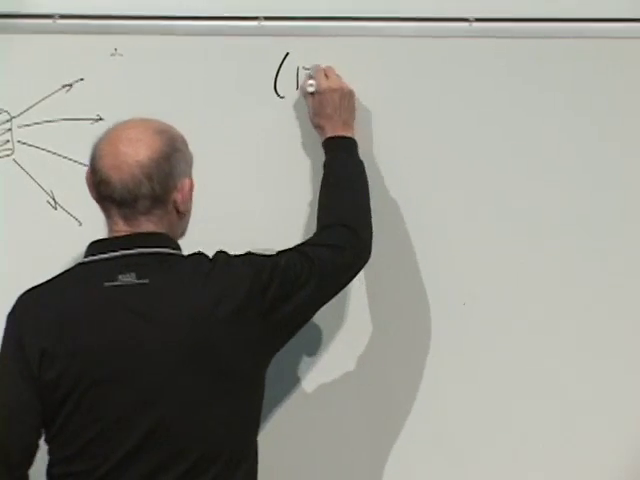
\includegraphics[width=0.66\textwidth]{lecture_06_figure_02.png}
  \caption{강의 전반에서 사용하는 계량 규약에서의 질량 껍질 조건.}
  \lectureframe{00:05:56}
  \label{fig:l06-mass-shell}
\end{figure}

운동량 \(k_1,k_2\)을 가진 입자 두 개가 들어오고, 물리적 운동량 \(q_3,q_4\)을 가진 입자 두 개가 나간다고 하자. 에너지와 운동량의 보존은 하나의 사차원 벡터 방정식으로 표현된다.
\begin{equation}
  k_1+k_2=q_3+q_4.
  \label{eq:l06-physical-conservation}
\end{equation}모든 외부선을 입사 운동량으로 나타내면 편리하다.
\begin{equation}
  k_3\equiv-q_3,
  \qquad
  k_4\equiv-q_4.
\end{equation}그러면
\begin{equation}
  k_1+k_2+k_3+k_4=0,
  \label{eq:l06-all-incoming}
\end{equation}이고 각 다리는 \(k_i^2=-m_i^2\)을 만족한다. 이 장부 기록 규약에서만 산란 입자들의 에너지가 음수로 나타난다. 물리적 에너지는 여전히 양수다.

\begin{figure}[H]
  \centering
  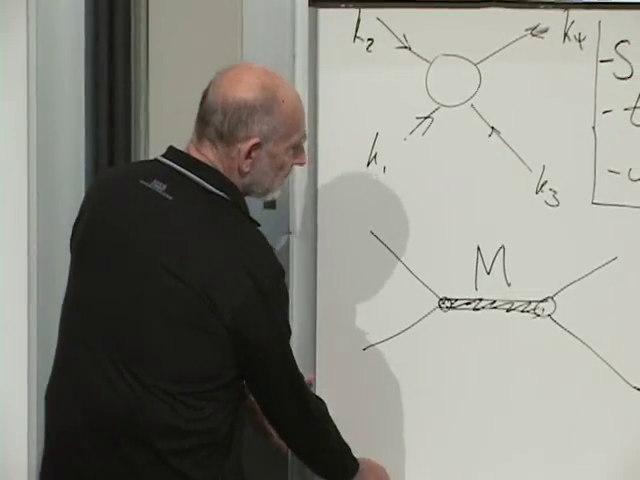
\includegraphics[width=0.68\textwidth]{lecture_06_figure_03.png}
  \caption{네 개의 외부 운동량을 대칭적으로 모두 입사로 다루도록, 물리적 산란 운동량의 방향을 뒤집는다.}
  \lectureframe{00:09:10}
  \label{fig:l06-all-incoming-board}
\end{figure}

처음에는 진폭이 16개의 성분 \(\mathcal A(k_1,k_2,k_3,k_4)\)을 인자로 하는 것처럼 보인다. 하지만 대부분은 중복 정보다. 질량 중심계로 가서 입사 운동량을 선택한 축에 맞추고, 간단히 네 입자의 질량이 모두 같다고 하자. 그러면 입사 상태는 질량 중심 에너지라는 하나의 수로 정해진다. 산란 입자들의 공간 운동량은 크기가 같고 방향이 서로 반대여야 하며, 그 크기는 입사 쌍의 운동량 크기와 같아야 한다. 남는 것은 산란각 \(\theta\)뿐이다. 따라서 이 과정에는 독립적인 운동학적 변수가 두 개 있다.
\begin{equation}
  E_{\mathrm{cm}},
  \qquad
  \theta.
  \label{eq:l06-two-data}
\end{equation}

\section{만델스탐 변수}

\eqref{eq:l06-two-data}에 등장하는 두 물리량은 기준계를 선택하지 않고 표현할 수 있어야 한다. 전부 입사로 보는 규약에 따라 다음과 같이 정의하자.
\begin{equation}
  \begin{aligned}
    -s&=(k_1+k_2)^2,\\
    -t&=(k_1+k_3)^2,\\
    -u&=(k_1+k_4)^2.
  \end{aligned}
  \label{eq:l06-mandelstam}
\end{equation}질량 중심계에서는 \(k_1+k_2\)의 공간 성분들이 상쇄되므로
\begin{equation}
  s=E_{\mathrm{cm}}^2.
  \label{eq:l06-s-energy}
\end{equation}

산란된 물리적 운동량 \(q_3=-k_3\)에 대해,
\begin{equation}
  k_1+k_3=k_1-q_3
\end{equation}는 다리 1에서 다리 3로 전달된 운동량이다. 외부 입자들의 질량이 같고 입사 공간 운동량의 크기가 \(p\)일 때,
\begin{equation}
  -t=2p^2(1-\cos\theta),
  \qquad
  -u=2p^2(1+\cos\theta).
  \label{eq:l06-tu-angle}
\end{equation}따라서 \(t\)와 \(u\)는 검출기로 측정하는 각도 정보를 담는다.

\begin{figure}[H]
  \centering
  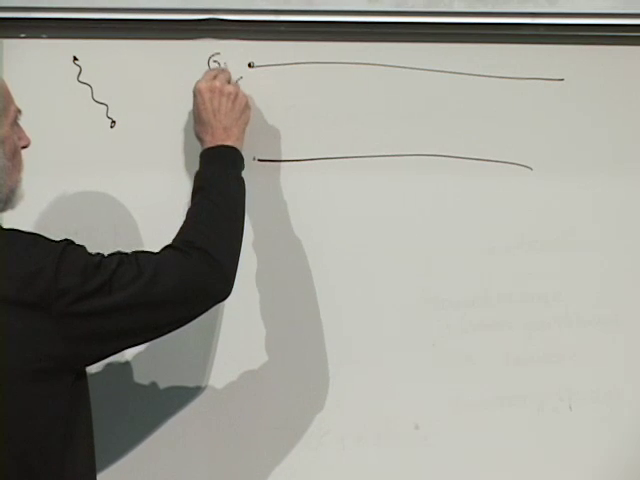
\includegraphics[width=0.74\textwidth]{lecture_06_figure_04.png}
  \caption{전부 입사 규약에서 \(s,t,u\)를 대칭적으로 정의한 식.}
  \lectureframe{00:26:20}
  \label{fig:l06-stu-board}
\end{figure}

기호가 세 개라고 해서 독립적인 정보도 세 가지인 것은 아니다. \eqref{eq:l06-all-incoming}을 제곱하고 \(k_i^2=-m^2\)을 사용하면 질량이 같은 경우
\begin{equation}
  s+t+u=4m^2
  \label{eq:l06-stu-constraint}
\end{equation}을 얻는다. \(s\)과 \(t\)을 알면 \(u\)은 정해진다.

\begin{classroomqa}
\audiencequestion{진공이 마찰처럼 작용해 자유롭게 움직이는 입자를 느리게 할 수 있을까요? \lecturetimestamp{00:27:17}}
\lecturerresponse{병진 대칭인 진공에서는 그럴 수 없습니다. 잃어버린 운동량이 갈 곳이 없으므로 운동량 보존이 그런 마찰을 금지합니다. 매질이나 선호하는 정지 기준계를 정하는 다른 진공을 생각할 수는 있지만, 여기서 다루는 진공은 그런 진공이 아닙니다.}
\end{classroomqa}

\begin{classroomqa}
\audiencequestion{산란된 두 입자의 에너지는 왜 같아야 하나요? \lecturetimestamp{00:27:54}}
\lecturerresponse{질량 중심계에서 두 입자의 공간 운동량은 크기가 같고 방향이 서로 반대여야 합니다. 여기서 다루는 과정처럼 두 입자의 질량이 같으면, 운동량 크기가 같으므로 \(E^2=p^2+m^2\)에 따라 에너지도 같습니다. 산란 입자들의 질량이 서로 다르다면 이 결론은 수정되어야 합니다.}
\end{classroomqa}

\section{직접 채널과 교차 채널}

단순한 점입자 도표에서는 입자 1과 2이 질량 \(M\)인 중간 입자를 만들고, 이 입자가 다시 3과 4로 붕괴할 수 있다. 분자 인자와 극점 처방을 제외하면 이 과정의 특징적인 의존성은 다음과 같다.
\begin{equation}
  \mathcal A_s\sim\frac{g^2}{s-M^2}.
  \label{eq:l06-s-channel}
\end{equation}이는 직접 채널, 즉 \(s\) 채널 과정이다. 연결 관계를 옆으로 돌리면 두 외부선 사이의 교환이 된다.
\begin{equation}
  \mathcal A_t\sim\frac{g^2}{t-M^2},
  \label{eq:l06-t-channel}
\end{equation}이는 교차 채널, 즉 \(t\) 채널 과정이다. 세 번째 연결 관계는 다음과 같다.
\begin{equation}
  \mathcal A_u\sim\frac{g^2}{u-M^2}.
  \label{eq:l06-u-channel}
\end{equation}

\begin{figure}[H]
  \centering
  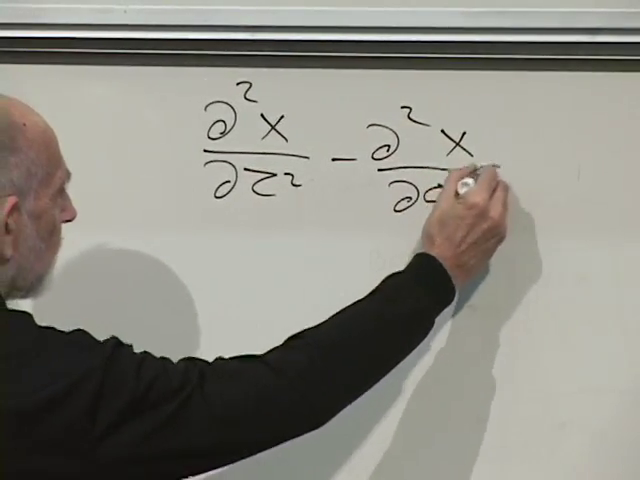
\includegraphics[width=0.72\textwidth]{lecture_06_figure_05.png}
  \caption{중간 상태를 통한 직접 생성과 이에 대응하는 극점 \(g^2/(s-M^2)\). 같은 판 위에 교차 채널의 연결 관계도 구성하고 있다.}
  \lectureframe{00:30:50}
  \label{fig:l06-channel-board}
\end{figure}

이 구분은 물리적이다. 이렇게 조잡한 스칼라 수준에서는 \eqref{eq:l06-s-channel}이 충돌 에너지에는 의존하지만 각도에는 의존하지 않는다. 복합 상태는 붕괴하기 전에 입사 방향에 대한 정보를 잃으므로 붕괴는 등방적이다. 교환 진폭은 운동량 전달에 의존하므로 각도에도 의존한다. 교환 입자의 질량이 작으면 산란각이 작아지는 과정이 강하게 우세해진다. 스핀을 고려하면 각도 의존성이 더 생기지만, 극점 구조는 이미 드러나 있다.

\begin{classroomqa}
\audiencequestion{빠진 \(u\) 채널에서도 세 번째 항이 생기나요? \lecturetimestamp{00:34:47}}
\lecturerresponse{입자의 종류와 결합이 그 연결 관계를 허용하면 생깁니다. 그러면 \(u=M^2\)에 극점을 갖는 항을 포함합니다. \(s+t+u=4m^2\)이므로 이것은 새로운 독립 운동학 변수가 아니지만, 별개의 채널 도표입니다.}
\end{classroomqa}

\section{하나의 함수, 두 가지 채널 기술}

하나의 극점만으로는 중간자 산란을 제대로 설명하기 어렵다. 두 중간자는 질량과 각운동량이 서로 다른 여러 공명 상태를 만들 수 있다. 1960년대에는 우선 \(s\) 채널 극점과 \(t\) 채널 극점을 더하고, 허용되는 \(u\) 채널 극점도 추가하는 방식으로 대응했다. 그러다가 훨씬 간결한 함수가 발견되었다. 선형 레제 궤적과 절편을 \(s\)와 \(t\)에 흡수한 강의의 단위계에서는 다음과 같다.
\begin{equation}
  \mathcal A_{\mathrm V}(s,t)
  \propto
  \frac{\Gamma(-s)\Gamma(-t)}{\Gamma(-s-t)}.
  \label{eq:l06-veneziano}
\end{equation}감마 함수는 양의 정수에서 계승을 일반화한다.
\begin{equation}
  \Gamma(n)=(n-1)!
\end{equation}

\begin{figure}[H]
  \centering
  \includegraphics[width=0.68\textwidth]{lecture_06_figure_06.png}
  \caption{감마 함수들의 대칭적인 비로 쓴 베네치아노 진폭.}
  \lectureframe{00:42:25}
  \label{fig:l06-veneziano-board}
\end{figure}

\(\Gamma(-s)\)의 극점은 무한한 직접 채널 공명 탑을 재현한다. 그런데 같은 식은 \(s\leftrightarrow
t\)에 대해 대칭이므로, \(\Gamma(-t)\)의 극점들은 교차 채널 전개도 제공한다. 이 두 기여를 따로 더한 것이 아니다. 하나의 해석 함수가 두 가지 기술을 모두 허용한다. 이것이 직접 채널 공명과 교차 채널 교환 사이의 오래된 쌍대성 개념이다.

\begin{classroomqa}
\audiencequestion{어떻게 하나의 진폭이 두 채널의 합을 더하지 않고 모두 담을 수 있나요? \lecturetimestamp{00:43:32}}
\lecturerresponse{바로 그것이 놀라운 점입니다. 함수의 \(s\) 채널 극점 근방에서 전개하면 직접 공명들로 정리되고, \(t\) 채널 극점 근방에서 전개하면 같은 함수가 교환 과정들로 정리됩니다. 이 두 해석이 왜 같은지를 설명하려면 미시적 모형이 필요하며, 그 모형이 상호작용하는 끈입니다.}
\end{classroomqa}

\section{열린 끈이 쓸어 만드는 띠}

열린 끈을 다음과 같이 매개화하자.
\begin{equation}
  0\leq\sigma\leq\pi.
\end{equation}표지 \(\sigma\)는 시공간 위치가 아니다. 매장 \(X^\mu(\sigma,\tau)\)은 그 표지가 붙은 점이 시공간의 어디에 놓이는지를 나타내며, \(\tau\)는 시간에 따른 변화를 나타낸다. 점입자가 쓸어 만드는 것은 세계선이고, 움직이는 끈은 2차원 세계면을 쓸어 만든다. 자유 이론에서는 각 매장 좌표가 다음 방정식을 만족한다.
\begin{equation}
  \frac{\partial^2X^\mu}{\partial\tau^2}
  -
  \frac{\partial^2X^\mu}{\partial\sigma^2}
  =0.
  \label{eq:l06-wave-equation}
\end{equation}

\begin{figure}[H]
  \centering
  \includegraphics[width=0.70\textwidth]{lecture_06_figure_07.png}
  \caption{세계면 띠 위에서 각 자유 끈 좌표를 지배하는 파동 방정식.}
  \lectureframe{00:49:10}
  \label{fig:l06-wave-equation-board}
\end{figure}

산란 과정을 구성할 때는 연속체 극한을 너무 일찍 취하지 않는 편이 유용하다. 각 끈을 스프링으로 연결된 질량점 \(n\)개로 바꾸자. 세계면은 서로 가까운 세계선들이 빽빽이 모인 형태가 되고, 정상 모드는 보통의 조화 진동자가 된다. 두 입사 사슬은 끝점에서 맞닿을 수 있다. 그 순간 새 스프링이 두 사슬을 연결해 하나의 더 긴 사슬로 만들고, 그 사슬은 시간 \(\tau\) 동안 진화한다. 나중에 스프링이 끊어지면 산란 사슬 두 개가 나온다.

\begin{figure}[H]
  \centering
  \includegraphics[width=0.72\textwidth]{lecture_06_figure_08.png}
  \medskip

  \begin{tikzpicture}[x=0.85cm,y=0.70cm]
    \draw[thick] (0,2.2) -- (2.1,2.2) -- (3.1,1.5);
    \draw[thick] (0,0.8) -- (2.1,0.8) -- (3.1,1.5);
    \draw[thick] (3.1,1.5) -- (5.5,1.5);
    \draw[thick] (5.5,1.5) -- (6.5,2.2) -- (8.6,2.2);
    \draw[thick] (5.5,1.5) -- (6.5,0.8) -- (8.6,0.8);
    \draw[<->] (3.1,0.35) -- node[below] {\(\tau\)} (5.5,0.35);
    \node[left] at (0,2.2) {1};
    \node[left] at (0,0.8) {2};
    \node[right] at (8.6,2.2) {3};
    \node[right] at (8.6,0.8) {4};
  \end{tikzpicture}
  \caption{이산화한 열린 끈 두 개가 맞닿아 하나의 중간 끈을 이루고, 시간 \(\tau\) 동안 지속된 뒤 분리된다. 원본 화면은 스프링과 세계선으로 구성된 그림을 보존하며, 도식은 그 연결 관계를 따로 보여 준다.}
  \lectureframe{00:51:25}
  \label{fig:l06-string-joining}
\end{figure}

두 끈은 매개변수 공간에서만 나란히 그려져 있다. 끝점 좌표가 실제로 일치하기 전까지 두 끈의 시공간 위치는 서로 가까울 필요가 없다. 재매개화 자유도를 이용하면 도표에서 결합과 분리 사건을 편리한 위치에 놓을 수 있다. 이 기하학적 자유도는 다음 강의에서 등각 대칭으로 나타난다.

\section{진동자 계산을 천천히 따라가기}

첫 번째 사슬의 좌표를 \(x_1,\ldots,x_n\), 두 번째 사슬의 좌표를 \(x_{n+1},\ldots,x_{2n}\)라 하자. 두 사슬의 질량 중심 좌표는 다음과 같다.
\begin{equation}
  X_{\mathrm{cm}}^{(1)}
  =\frac1n\sum_{a=1}^{n}x_a,
  \qquad
  X_{\mathrm{cm}}^{(2)}
  =\frac1n\sum_{a=n+1}^{2n}x_a.
  \label{eq:l06-chain-centers}
\end{equation}운동량이 정해진 \(k_1\)을 가진 사슬의 파동함수는 질량 중심 평면파에 내부 진동자의 바닥 상태를 곱한 형태다.
\begin{align}
  \Psi_1
  &=
  e^{ik_1\cdot X_{\mathrm{cm}}^{(1)}}
  \psi_0(x_1,\ldots,x_n),
  \\
  \Psi_2
  &=
  e^{ik_2\cdot X_{\mathrm{cm}}^{(2)}}
  \psi_0(x_{n+1},\ldots,x_{2n}).
  \label{eq:l06-two-wavefunctions}
\end{align}인자 \(\psi_0\)는 상대 좌표에 의존하며, 사슬 전체를 함께 평행 이동시키는 데에는 의존하지 않는다. 입사 끈들은 처음에 서로 독립된 양자계이므로
\begin{equation}
  \Psi_{\mathrm{in}}=\Psi_1\Psi_2.
  \label{eq:l06-product-state}
\end{equation}

\begin{figure}[H]
  \centering
  \includegraphics[width=0.76\textwidth]{lecture_06_figure_09.png}
  \caption{두 운동량 평면파와 내부 진동자 바닥 상태 인자. 서로 다른 색으로 표시되어 있다.}
  \lectureframe{00:58:05}
  \label{fig:l06-wavefunctions-board}
\end{figure}

결합은 두 끝점 좌표가 일치하는 파동함수 성분을 선택한다.
\begin{equation}
  x_n=x_{n+1}.
  \label{eq:l06-endpoint-contact}
\end{equation}그 순간 다른 좌표들은 변하지 않는다. 그런 다음 선택된 상태는 더 긴 단일 사슬의 해밀토니안 \(H_{\mathrm{joined}}\)에 따라 진화한다.
\begin{equation}
  \Psi(\tau)
  =
  e^{-iH_{\mathrm{joined}}\tau}\Psi(0).
  \label{eq:l06-time-evolution}
\end{equation}마지막으로 운동량 \(q_3,q_4\)을 가진 산란 끈 상태들의 곱과 겹침을 취한다.

\begin{figure}[H]
  \centering
  \includegraphics[width=0.76\textwidth]{lecture_06_figure_10.png}
  \caption{끝점의 일치를 부과하기 직전 두 사슬의 파동함수.}
  \lectureframe{00:58:55}
  \label{fig:l06-endpoint-board}
\end{figure}

계산은 길지만 신비롭지는 않다. 각 내부 좌표를 진동자 모드로 분해할 수 있으므로, 결합 겹침과 시간 진화, 마지막 사영은 가우스 진동자 대수로 환원된다. 아직 정해지지 않은 것은 결합된 끈의 지속 시간 \(\tau\)이다.

\begin{classroomqa}
\audiencequestion{검은색과 빨간색 파동함수는 더하나요, 곱하나요? \lecturetimestamp{01:02:26}}
\lecturerresponse{곱합니다. 독립된 두 계의 텐서곱 상태는 좌표 기저에서 각 파동함수의 곱으로 표현됩니다. 더하기는 두 입사 끈이 동시에 존재하는 상황이 아니라 여러 대안의 중첩을 나타냅니다.}
\end{classroomqa}

\begin{classroomqa}
\audiencequestion{중간 시간 \(\tau\)에 대해 적분하는 이유는 무엇인가요? \lecturetimestamp{01:04:04}}
\lecturerresponse{결합된 끈에 정해진 지속 시간을 부여하지 않습니다. 파인만의 규칙에 따르면 허용되는 모든 역사에 대한 진폭을 합산합니다. 이 기술에서 남아 있는 연속적인 역사 매개변수가 결합과 분리 사이의 시간이므로, 합산은 \(0\leq\tau<\infty\)에 대한 적분이 됩니다.}
\end{classroomqa}

\section{전파 시간에서 베타 함수까지}

진동자 겹침을 계산하고 나면 결과를 다음과 같이 정리할 수 있다.
\begin{equation}
  \mathcal A(s,t)
  \propto
  \int_0^\infty d\tau\,
  e^{\tau(s+1)}
  \bigl(1-e^{-\tau}\bigr)^{-t-1}
  e^{-\tau}.
  \label{eq:l06-tau-integral}
\end{equation}마지막 \(e^{-\tau}\) 인자는 다음 단계에서 필요한 야코비안이므로 그대로 표시해 둔다. 이에 대응해 첫 번째 지수함수와 마지막 지수함수를 합치면 \(e^{s\tau}\)이 된다.

\begin{figure}[H]
  \centering
  \includegraphics[width=0.76\textwidth]{lecture_06_figure_11.png}
  \caption{진동자 계산 뒤의 전파 시간 적분식. 별도로 표시된 \(e^{-\tau}\) 인자는 변수 변환에 필요한 야코비안을 제공한다.}
  \lectureframe{01:06:45}
  \label{fig:l06-tau-integral-board}
\end{figure}

이제 다음과 같이 두자.
\begin{equation}
  z=e^{-\tau},
  \qquad
  dz=-e^{-\tau}\,d\tau.
  \label{eq:l06-z-substitution}
\end{equation}\(\tau\)이 \(0\)에서 \(\infty\)까지 변할 때, \(z\)는 \(1\)에서 \(0\)까지 변한다. 음수 부호 때문에 적분 구간의 순서가 뒤집히므로
\begin{equation}
  \mathcal A(s,t)
  \propto
  \int_0^1
  z^{-s-1}(1-z)^{-t-1}\,dz.
  \label{eq:l06-beta-integral}
\end{equation}

\begin{figure}[H]
  \centering
  \includegraphics[width=0.74\textwidth]{lecture_06_figure_12.png}
  \caption{치환 \(z=e^{-\tau}\)으로 오일러 베타 적분이 드러난다.}
  \lectureframe{01:08:49}
  \label{fig:l06-beta-integral-board}
\end{figure}

이 적분은 양 끝점에서 수렴하는 영역에서 직접 정의하고, 그 밖의 영역에서는 해석적 연속으로 정의한다. 이것은 오일러 베타 함수다.
\begin{equation}
  B(-s,-t)
  =
  \frac{\Gamma(-s)\Gamma(-t)}{\Gamma(-s-t)}.
  \label{eq:l06-beta-gamma}
\end{equation}

\begin{figure}[H]
  \centering
  \includegraphics[width=0.72\textwidth]{lecture_06_figure_13.png}
  \caption{칠판의 적분을 \(B(-s,-t)\)로 확인하고 감마 함수 형태를 복원하기 시작한다.}
  \lectureframe{01:12:24}
  \label{fig:l06-beta-gamma-board}
\end{figure}

이제 채널 대칭은 간단히 확인할 수 있다. \(z\mapsto1-z\)에 따라
\begin{equation}
  \int_0^1 z^{-s-1}(1-z)^{-t-1}\,dz
  =
  \int_0^1 z^{-t-1}(1-z)^{-s-1}\,dz.
\end{equation}따라서 \(\mathcal A(s,t)=\mathcal A(t,s)\)이다. 두 끈이 결합한 뒤 다시 분리되는 과정으로부터 교차 채널에 대한 기술도 자동으로 포함된다.
\editorialnote{강의에서는 베타 함수의 인자에서 레제 기울기와 절편을 생략한다. 표준 표기에서는 \(s,t\)를 그에 대응하는 선형 궤적 \(\alpha(s),\alpha(t)\)로 바꾼다. 쌍대성과 변수 변환 논리는 그대로다.}

\begin{classroomqa}
\audiencequestion{감마 함수의 비가 조합론의 계승 표현과 닮았습니다. 이를 직접적인 물리적 계수로 해석할 수 있나요? \lecturetimestamp{01:13:22}}
\lecturerresponse{정수 인자에서 베타 함수가 \(n!\,m!/(n+m)!\) 같은 비와 관계되는 것은 맞지만, 여기서 조합론적 메커니즘을 주장하는 것은 아닙니다. 같은 특수 함수가 세계면 적분에서도 나타난다는 뜻일 뿐입니다. 이런 유사성을 바탕으로 진폭을 발견한 것은 아닙니다.}
\end{classroomqa}

하나의 세계면을 두 채널로 해석할 수 있는 이유는 아직 다루지 않은 등각 대칭에 있다. 등각 대칭을 이용하면 진폭을 바꾸지 않고 세계면을 늘였다 줄일 수 있어, 긴 직접 채널 전파 영역을 교차 채널 교환 그림으로 바꿀 수 있다. 이 기하학적 설명은 다음 강의에서 다룬다.

\section{산란 검증으로 확인한 것}\enlargethispage{3\baselineskip}\begingroup
\setlength{\medskipamount}{3pt plus 1pt minus 1pt}

이산적인 결합 그림은 마지막 몇 가지 질문을 불러왔다.

\begin{classroomqa}
\audiencequestion{\(n\)개의 구성 요소를 가진 두 사슬이 끝점에서 결합하면 결과의 구성 요소 수는 \(2n-1\)이 되나요? 페르미온 패리티가 바뀔 가능성은 없나요? \lecturetimestamp{01:16:16}}
\lecturerresponse{하드론의 끝점 그림에서는 맞닿은 끝점 쌍을 소멸하는 입자·반입자 쌍으로 볼 수 있으므로, 수는 1이 아니라 2만큼 줄어듭니다. 연속체 극한에서는 \(2n\)와 \(2n-2\) 사이의 유한한 차이는 중요하지 않지만, 페르미온 패리티를 보존하는 것은 중요합니다. 격자 구성 요소는 연속적인 끈을 위한 정규화 도구일 뿐, 실제로 존재하는 기본 구슬이 아닙니다.}
\end{classroomqa}

\begin{classroomqa}
\audiencequestion{이후 논의에서는 초끈 이론의 수학 전반까지 다루게 되나요? \lecturetimestamp{01:18:05}}
\lecturerresponse{선별된 결과만 활용할 것이다. 먼저 세계면 대칭성과 콤팩트화를 살펴본 다음, 1990년대 중반에 발전한 또 다른 출발점인 M이론으로 나아간다. M이론의 목적은 다른 경우에는 복잡한 여러 특징이 투명하게 드러나는 관점에서 동일한 물리에 도달하는 것이다.}
\end{classroomqa}

\begin{classroomqa}
\audiencequestion{이 결합 규칙은 중간자 충돌에서 얻은 단서에 불과했나요? \lecturetimestamp{01:20:02}}
\lecturerresponse{중간자 산란이 역사적 단서를 제공했지만, 이 규칙은 열린 끈 전반에 적용된다. 같은 위상 구조는 열린 끈 광자와 다른 열린 끈 상태들의 충돌도 기술한다. 두 닫힌 끈은 중간 영역에 닫힌 끈이 놓이는 유사한 구성으로 결합하고 분리된다.}
\end{classroomqa}

\begin{classroomqa}
\audiencequestion{이 계산은 끈 상태가 페르미온인 경우에만 적용되나요? \lecturetimestamp{01:20:56}}
\lecturerresponse{아닙니다. 원래의 베네치아노 계산은 보손 열린 끈에 관한 것입니다. 초끈에서는 페르미온 자유도를 추가해야 하고 적분식의 세부 형태도 달라지지만, 결합과 전파, 사영, 세계면 쌍대성의 논리는 매우 유사하게 유지됩니다.}
\end{classroomqa}

진동자 스펙트럼에서 스핀 1 또는 스핀 2 상태를 발견한 것은 시사적이었지만 결정적이지는 않았다. 이 상태들의 산란 진폭이 더 강력한 검증을 제공했다. 광자 진폭은 전하 보존과 게이지 불변성에 관련된 항등식을 만족하고, 중력자 진폭은 질량 없는 스핀 2 장에 대응하는 제약을 만족한다. 끈 상태는 질량이 있는 상태와 없는 상태, 그리고 서로 간의 상호작용에서 이 검증을 통과했다. 그래서 광자와 중력자라는 이름은 편광 개수를 보고 한 추측이 아니라 물리적 동정이 되었다.
\editorialnote{현대적 표현으로는 비물리적 편광의 분리, 게이지 워드 항등식, 질량 없는 스핀 2 상태의 보편적인 저에너지 결합이 이러한 검증을 이룬다.}

\begin{classroomqa}
\audiencequestion{끈 이론에서 전하 자체는 어디서 나오나요? \lecturetimestamp{01:24:03}}
\lecturerresponse{강의 마지막에서도 이 질문에는 답하지 않는다. 답하려면 아직 도입되지 않은 끈 이론의 내부 구조와 끝점 구조가 필요하므로, 이 산란 유도 과정이 아니라 이어지는 논의에서 다뤄야 한다.}
\end{classroomqa}
\endgroup

\chapter{세계면, Wick 회전, 채널 쌍대성}

\lectureoverview{입자는 세계선을 따라 움직이고, 끈은 세계면을 쓸고 지나간다. 어느 쪽을 양자화하든 모든 역사를 합산해야 하지만, 로런츠 부호수에서의 합은 진동적이어서 정의하기 어렵다. 세계면의 시간을 허수 좌표로 바꾸면 라플라스 방정식이 지배하는 유클리드 이론을 얻는다. 이어서 등각 대칭을 이용하면 네 끈 상호작용의 슬릿 표면을 경계 삽입점 네 개가 있는 원판으로 바꿀 수 있으며, 이때 직접 채널과 교차 채널 사이의 대칭성이 드러난다.}

\section{세계선에서 역사 합산으로}

자유 입자부터 시작하자. 비상대론적 역학에서 입자의 위치는 함수 \(\mathbf x(t)\)이며, 질량을 1로 두면 작용은 다음과 같다.
\begin{equation}
  S_{\mathrm{NR}}[\mathbf x]
  =\frac12\int_{t_1}^{t_2}\dot{\mathbf x}^{\,2}\,dt.
  \label{eq:l07-nr-action}
\end{equation}
상대론적으로 기술할 때는 시간과 공간을 하나의 벡터 \(X^\mu(\tau)\)에 넣고, 궤적을 따라 매개화 변수 \(\tau\)를 사용하는 편이 더 자연스럽다. 이에 대응하는 이차식은 다음과 같다.
\begin{equation}
  S_{\mathrm{rel}}[X]
  =\frac12\int_{\tau_1}^{\tau_2}
  \frac{dX^\mu}{d\tau}\frac{dX_\mu}{d\tau}\,d\tau.
  \label{eq:l07-rel-action}
\end{equation}
위 첨자와 아래 첨자는 시간과 공간 사이의 로런츠 부호 차이를 나타낸다.
\editorialnote{여기서는 고정된 세계선 매개화에서 이차 상대론적 작용을 사용한다. 매개화 불변성이 명시적으로 드러나는 대안은 고유 길이에 비례하는 작용이며, 강의 뒤에서 언급한다.}

\begin{figure}[H]
  \centering
  \includegraphics[width=0.72\textwidth]{lecture_07_figure_01.png}
  \caption{칠판에 함께 적힌 비상대론적 작용과 이에 대응하는 상대론적 이차 작용.}
  \lectureframe{00:03:35}
  \label{fig:l07-particle-actions}
\end{figure}

고전적으로는 양 끝점을 고정하고 경로를 변분한다. 그러면 자유 입자는 일정한 속도로 직선 세계선을 따른다. 양자역학은 다른 질문을 던진다. 양 끝점 사이의 궤적 하나를 선택하는 것이 아니라, 한 점에서 시작해 다른 점에서 검출될 진폭을 묻는다. 그 사이를 지나는 모든 경로가 위상 인자를 기여한다.
\begin{equation}
  K(2,1)=\int_{X(1)}^{X(2)}\!\mathcal D X\,
  e^{iS[X]}.
  \label{eq:l07-feynman-integral}
\end{equation}
범함수 적분은 경로들이 이루는 무한차원 공간에 대한 적분이다. 작용 안에 이미 들어 있는 통상적인 적분과는 다르다.

\begin{figure}[H]
  \centering
  \includegraphics[width=0.72\textwidth]{lecture_07_figure_02.png}
  \caption{모든 궤적을 합산하기 전에 대표 경로 하나와 그 경로에 부여된 위상.}
  \lectureframe{00:06:21}
  \label{fig:l07-path-integral-board}
\end{figure}

상대론적 표현에서 이 점과 점 사이의 진폭은 전파자다. 상호작용에서는 여러 세계선 구간이 한 점에서 만난다. 각 구간의 작용을 더하고, 만나는 점들에 대해 적분하며, 필요한 외부 입자들을 포함하는 도표들을 합산한다. 따라서 익숙한 파인만 도표 전개는 이미 역사를 합산하라는 지시에 내포되어 있다.

여기서는 작용을 \(S\)로 표기한다. 이 표기는 엔트로피와도, 강의 끝부분에서 쓰는 만델스탐 변수 \(s\)와도 관계가 없다. 표기가 같은 것은 설명에 도움이 되기 때문이 아니라 관례에 따른 것이다.

\section{시간을 옆으로 돌리기}

\eqref{eq:l07-feynman-integral}에는 즉각적인 문제가 있다. 모든 인자 \(e^{iS}\)의 절댓값은 1이다. 따라서 크게 진동하는 궤적과 고전적인 직선 궤적이 절대값 기준으로 똑같은 가중치를 갖고, 위상만 다르다. 상쇄 간섭을 통해 고전적 거동이 나타나지만, 그렇다고 형식적인 적분이 통상적인 의미에서 수렴하는 것은 아니다.

다음 관계로 새 매개변수 \(s\)를 도입하자.
\begin{equation}
  \tau=\alpha s,
  \qquad
  d\tau=\alpha\,ds,
  \qquad
  \frac{dX}{d\tau}=\frac{1}{\alpha}\frac{dX}{ds}.
\end{equation}
그러면 이차 작용은 다음과 같이 재척도화된다.
\begin{equation}
  \frac12\int d\tau
  \left(\frac{dX}{d\tau}\right)^2
  =
  \frac{1}{2\alpha}\int ds
  \left(\frac{dX}{ds}\right)^2.
  \label{eq:l07-rescaled-action}
\end{equation}
\(\alpha=-i\)에 해당하는 적분 경로를 선택하면 진동하는 가중치가 다음과 같이 바뀐다.
\begin{equation}
  e^{iS}
  \longrightarrow
  \exp\!\left[-\frac12\int ds
  \left(\frac{dX}{ds}\right)^2\right]
  =e^{-S_E}.
  \label{eq:l07-euclidean-particle}
\end{equation}

\begin{figure}[H]
  \centering
  \includegraphics[width=0.66\textwidth]{lecture_07_figure_03.png}
  \caption{허수 시간 치환 후의 유클리드 입자 가중치. 지수는 실수이며 양수가 아니다.}
  \lectureframe{00:16:20}
  \label{fig:l07-particle-wick}
\end{figure}

멀리 달아났다가 돌아오는 경로나 멀리 이동하지 않으면서 빠르게 흔들리는 경로는 큰 양의 \(S_E\)를 가지므로 지수적으로 억제된다. 그 결과 위너형 적분을 얻으며, 이 적분에는 엄밀한 수렴 이론이 있다. 실수 \(\tau\)에서 물려받은 양 끝점은 허수 \(s\)-경로 위에 놓인다. 실제로는 수렴하는 영역에서 유클리드 대상을 계산한 뒤, 해를 해석적으로 연장하여 물리적인 로런츠 변수로 되돌린다. 이것이 Wick 회전이다. 계산을 위해 시간을 옆으로 돌린 것이지, 시간을 없앤 것은 아니다.

\section{세계선에서 세계면으로}

점 입자는 세계선을 이룬다. 열린 끈은 리본 모양의 면을 쓸고 지나가고, 닫힌 끈은 관 모양의 면을 쓸고 지나간다. 좌표 \((\sigma,\tau)\)는 이 2차원 세계면 위의 점을 표시하며,
\begin{equation}
  X^\mu=X^\mu(\sigma,\tau)
  \label{eq:l07-embedding}
\end{equation}
는 표시된 점의 시공간 위치를 나타낸다. 모든 함수 \(X^\mu\)를 알면 끈의 전체 역사가 정해진다.

로런츠 부호수에서의 이차 세계면 작용은 보통 진동하는 끈의 운동에너지에서 퍼텐셜 에너지를 뺀 구조와 같다.
\begin{equation}
  S_{\mathrm{ws}}[X]
  =\frac{T_s}{2}\int d\tau\,d\sigma\,
  \left[
    \partial_\tau X^\mu\partial_\tau X_\mu
    -
    \partial_\sigma X^\mu\partial_\sigma X_\mu
  \right].
  \label{eq:l07-lorentzian-worldsheet}
\end{equation}
전체 장력 \(T_s\)가 척도를 정한다. 이 강의에서는 미분항의 구조에 집중하기 위해 장력을 생략한다.

\begin{figure}[H]
  \centering
  \includegraphics[width=0.72\textwidth]{lecture_07_figure_04.png}
  \caption{운동에너지에서 퍼텐셜 에너지를 빼는 부호 구조를 갖는 \(X^\mu(\sigma,\tau)\)의 로런츠 세계면 작용.}
  \lectureframe{00:24:26}
  \label{fig:l07-worldsheet-action}
\end{figure}

끈의 진폭은 이 작용을 지수화하고, 주어진 초기 끈 상태와 최종 끈 상태를 잇는 모든 면에 대해 합산해 구한다.
\begin{equation}
  \mathcal A=\int\mathcal D X\,e^{iS_{\mathrm{ws}}[X]}.
  \label{eq:l07-surface-integral}
\end{equation}
이 규칙은 두 끈이 둘로 바뀌는 경우, 둘이 셋으로 바뀌는 경우, 그 밖의 허용된 외부 상태 구성에도 똑같이 적용된다. 서로 다른 세계면 위상도 합산에 포함된다. 구멍을 더하는 것은 점 입자 도표 전개에서 루프 차수를 더하는 것에 해당한다.

\begin{figure}[H]
  \centering
  \includegraphics[width=0.66\textwidth]{lecture_07_figure_05.png}
  \caption{여러 외부 끈을 잇는 면. 구멍은 서로 다른 세계면 위상을 나타낸다.}
  \lectureframe{00:27:14}
  \label{fig:l07-surface-topology}
\end{figure}

\begin{classroomqa}
\audiencequestion{점 전자의 경우 \(\sigma\)-미분은 그냥 사라지나요? \lecturetimestamp{00:27:56}}
\lecturerresponse{점 입자에는 애초에 \(\sigma\) 좌표가 없다. 그래도 두 그림은 서로 연결되어 있다. 외부 상태의 에너지가 끈 척도보다 작고 과정의 에너지도 낮으면, 끈 진폭은 보통의 점 입자 파인만 도표를 재현한다. 그 극한은 미분 하나를 0으로 두는 것 이상을 뜻한다.}
\end{classroomqa}

표면 적분에도 경로 적분과 같은 수렴 문제가 있다. 세계면 시간을 Wick 회전하면 안정적인 유클리드 형식은 다음과 같다.
\begin{equation}
  \begin{aligned}
    S_{E,\mathrm{ws}}[X]
    &=\frac{T_s}{2}\int d\tau\,d\sigma\,
      \left[
        \partial_\tau X^\mu\partial_\tau X_\mu
        +\partial_\sigma X^\mu\partial_\sigma X_\mu
      \right],\\
    \mathcal A_E&=\int\mathcal D X\,e^{-S_{E,\mathrm{ws}}}.
  \end{aligned}
  \label{eq:l07-euclidean-worldsheet}
\end{equation}
이제 두 미분항의 부호가 모두 양수다. 격렬하게 진동하거나 크게 늘어난 표면은 유클리드 작용이 크므로 억제된다.

\begin{figure}[H]
  \centering
  \includegraphics[width=0.72\textwidth]{lecture_07_figure_06.png}
  \caption{\(\tau\)를 허수 시간으로 회전한 뒤의 양의 유클리드 세계면 밀도.}
  \lectureframe{00:34:29}
  \label{fig:l07-worldsheet-wick}
\end{figure}

기하학적으로 더 직접적인 정식화도 있다. 상대론적 입자에는 경로의 고유 길이에 비례하는 작용을 부여할 수 있고, 끈에는 세계면의 시공간 넓이에 비례하는 작용을 부여할 수 있다. 후자는 Nambu--Goto 작용이다. 여기서 사용하는 이차 세계면 형식은 관례적으로 Polyakov 형식이라 부르며, 현재 계산에는 훨씬 다루기 쉽다.
\editorialnote{강의에서는 역사적 명명에 관한 유머러스한 이야기를 하며, 관련된 Liouville 작용과 Dirichlet 경계 조건도 언급한다. 유도 과정에 우선권 주장을 덧붙일 필요는 없다. 여기서 쓰는 것은 넓이 정식화와 보조 계량 정식화의 동등성뿐이다.}

\section{유클리드 운동 방정식}

좌표 \(\sigma\)와 \(\tau\)는 세계면 위의 표시에 불과하다. 그러므로 다음 질문은 피할 수 없다. 어떤 재표시 변환이 이론을 변하지 않게 하는가? 운동 방정식을 보면 답을 가장 쉽게 알 수 있다. \eqref{eq:l07-euclidean-worldsheet}를 변분하면 각 성분은 다음을 만족한다.
\begin{equation}
  \partial_\tau^2X^\mu+\partial_\sigma^2X^\mu=0.
  \label{eq:l07-laplace}
\end{equation}
Wick 회전 전에는 상대 부호가 음수이며, 이 식은 파동 방정식이다. 유클리드 부호수에서는 두 부호가 양수이므로 2차원 라플라스 방정식이 된다.

\begin{classroomqa}
\audiencequestion{이것은 진동하는 북의 방정식인가요?
\lecturetimestamp{00:41:50}}
\lecturerresponse{밀접한 관련은 있지만, 진동하는 북에는 실시간 좌표도 있으므로 파동 방정식을 따른다. 여기서의 방정식은 유클리드 라플라스 방정식이다. 전하가 없는 영역의 정전기 퍼텐셜이 더 직접적이고 익숙한 예다.}
\end{classroomqa}

\begin{classroomqa}
\audiencequestion{작용에는 1계 미분만 있는데 왜 운동 방정식에는 2계 미분이 들어가나요? \lecturetimestamp{00:42:44}}
\lecturerresponse{1계 미분의 제곱항을 변분한 뒤 부분 적분하면, 그 미분 하나가 그 1계 미분에 작용하도록 옮겨진다. 이는 작용의 \(\dot x^{\,2}\)가 운동 방정식의 \(\ddot x\)를 낳는다는 관계를 장 이론에 적용한 것이다.}
\end{classroomqa}

\begin{figure}[H]
  \centering
  \includegraphics[width=0.68\textwidth]{lecture_07_figure_07.png}
  \caption{플러스 부호의 라플라스 방정식과 그 2계 미분을 해석하는 데 처음 쓰이는 이산식.}
  \lectureframe{00:43:30}
  \label{fig:l07-laplace-board}
\end{figure}

기하학적 의미를 살펴보기 위해 먼저 한 좌표를 간격 \(\epsilon\)로 이산화하자. 1계 미분은 이웃한 값의 차이고, 2계 미분은 이웃한 차이들의 차이다.
\begin{equation}
  \frac{d^2X}{ds^2}\bigg|_{2}
  \longrightarrow
  \frac{X(3)-2X(2)+X(1)}{\epsilon^2}.
  \label{eq:l07-second-difference}
\end{equation}

\begin{figure}[H]
  \centering
  \includegraphics[width=0.72\textwidth]{lecture_07_figure_08.png}
  \caption{번호가 붙은 식, 작은 격자 영역, 2계 미분의 유한차분 전개.}
  \lectureframe{00:45:51}
  \label{fig:l07-finite-difference-board}
\end{figure}

이제 \((\sigma,\tau)\)-평면을 이산화하자. 중심점 \(5\)의 네 최근접 이웃을 \(1,2,3,4\)로 표시하자. \eqref{eq:l07-laplace}은 다음 식이 된다.
\begin{equation}
  X(1)+X(2)+X(3)+X(4)-4X(5)=0,
\end{equation}
또는
\begin{equation}
  X(5)=\frac14\bigl[X(1)+X(2)+X(3)+X(4)\bigr].
  \label{eq:l07-mean-value}
\end{equation}

\begin{figure}[H]
  \centering
  \includegraphics[width=0.72\textwidth]{lecture_07_figure_09.png}
  \caption{완성된 2차원 유한차분 방정식. 중심값은 네 이웃값의 평균이다.}
  \lectureframe{00:48:26}
  \label{fig:l07-mean-value-board}
\end{figure}

이 평균값 성질은 어떤 방향의 무한소 정사각형에도 성립한다. 이것이 라플라스 방정식의 국소적인 기하학적 내용이며, 등각 대칭으로 이어지는 연결고리다.

\section{등각 좌표}

\((\sigma,\tau)\)에서 \((\sigma',\tau')\)로의 변환을 생각하자. 일반적인 변형은 작은 정사각형을 임의의 사각형으로 보낸다. 여기서 다룰 특별한 변환은 모든 무한소 정사각형을, 회전하거나 크기가 변할 수는 있지만, 또 다른 무한소 정사각형으로 보낸다. 바꾸어 말하면 곡선들이 만나는 각을 보존한다. 이런 변환을 등각 변환이라 한다.

\begin{figure}[H]
  \centering
  \includegraphics[width=0.68\textwidth]{lecture_07_figure_10.png}
  \caption{국소 정사각형이 다른 작은 도형으로 사상될 때 각이 보존되는지 살펴보는 그림.}
  \lectureframe{00:53:25}
  \label{fig:l07-conformal-board}
\end{figure}

\begin{classroomqa}
\audiencequestion{각이 보존된다면 변환은 사실상 회전만을 뜻하나요? \lecturetimestamp{00:53:31}}
\lecturerresponse{국소적으로만 그렇고, 그 경우에도 공통적인 크기 변화가 허용된다. 국소 회전과 축척 인자는 점마다 달라질 수 있으므로, 무한소 도형의 모양을 보존하면서 좌표 격자는 휘고 어떤 영역에서는 늘어나며 다른 영역에서는 줄어들 수 있다.}
\end{classroomqa}

각을 보존하는 사상이 크기까지 보존할 필요는 없다. 크기도 모든 곳에서 보존된다면 가능한 변환은 평행이동과 회전이라는 훨씬 제한적인 강체 변환으로 줄어든다. 반면 등각 사상은 국소적인 모양을 보존한다. 그래서 지도 투영은 작은 섬의 모양을 유지하면서도 면적을 크게 왜곡할 수 있다.

\begin{classroomqa}
\audiencequestion{등각 사상은 좌표계가 평탄하다는 뜻인가요? \lecturetimestamp{00:55:35}}
\lecturerresponse{아니다. 평탄성과 등각성은 서로 다른 주장이다. 등각 사상은 휘어진 좌표선을 사용할 수 있다. 보존되는 것은 교차하는 곡선 사이의 각이다. 메르카토르형 지도 투영은 국소적인 모양을 보존하면서 축척을 크게 왜곡하는 익숙한 예다.}
\end{classroomqa}

2차원에서 필요한 변환은 복소 좌표의 해석 함수에 의해 국소적으로 생성된다.
\begin{equation}
  z=\sigma+i\tau.
\end{equation}
유한한 경계는 겉모습이 크게 달라질 수 있다. 정사각형 영역이 매끄러운 영역으로 사상되면, 원래의 모서리는 새 경계에서 눈에 띄는 점이 아니라 평범한 점으로 옮겨질 수 있다. 모순은 없다. 등각성은 내부에서 성립하는 국소 조건이며, 사상이 정칙인 곳에서는 무한소 각을 보존한다.

\begin{classroomqa}
\audiencequestion{이런 좌표 자유도가 앞서 다룬 결합--분리 도표를 대칭적으로 그릴 수 있었던 이유인가요?
\lecturetimestamp{00:56:32}}
\lecturerresponse{그렇다. 세계면 방정식을 보존하는 동일한 등각 자유도 덕분에 다루기 까다로운 상호작용 띠를 더 대칭적인 영역으로 바꿀 수 있다. 남아 있는 자유도는 물리적인 결합--분리 매개변수를 없애지 않는다. 대신 경계 삽입점들의 상대적 위치로 다시 나타낸다.}
\end{classroomqa}

\section{슬릿 세계면과 원판}

네 끈 산란으로 돌아가자. 열린 끈 두 개가 들어와 그 끝점들이 결합하고, 결합된 끈이 전파된 다음, 나중에 분리된다. 평평한 세계면으로 그리면 양쪽 끝에서 슬릿이 난 무한 띠가 된다. 슬릿 끝 사이의 거리 \(\tau_0\)는 중간 끈의 수명이며, 진폭은 이 값에 대해 적분한다.

\begin{figure}[H]
  \centering
  \includegraphics[width=0.72\textwidth]{lecture_07_figure_11.png}
  \caption{열린 끈 두 개가 결합해 함께 전파된 뒤 다시 분리되는 과정을 나타내는 양쪽에 슬릿이 난 띠.}
  \lectureframe{01:00:20}
  \label{fig:l07-slit-strip}
\end{figure}

유클리드화한 뒤 이 영역의 매장장은 라플라스 방정식을 만족한다. 따라서 등각 불변성을 이용해 슬릿 띠를 원판으로 사상할 수 있다. 위상을 이해하는 한 가지 방법은 원판을 동심원들로 엽층화한 다음, 이 닫힌 곡선들을 연속적으로 변형해 슬릿 영역 전체를 채우는 것이다. 사상 아래에서 무한대에 있던 끝점들은 예외적인 경계점이 된다.

\begin{figure}[H]
  \centering
  \includegraphics[width=0.72\textwidth]{lecture_07_figure_12.png}
  \medskip

  \begin{adjustbox}{max width=\linewidth}
  \begin{tikzpicture}[x=0.75cm,y=0.75cm]
    \draw[thick] (-5,1.2) -- (-1.2,1.2) -- (-0.35,0.35);
    \draw[thick] (-5,-1.2) -- (-1.2,-1.2) -- (-0.35,-0.35);
    \draw[thick] (0.35,0.35) -- (1.2,1.2) -- (5,1.2);
    \draw[thick] (0.35,-0.35) -- (1.2,-1.2) -- (5,-1.2);
    \draw[->,thick] (5.6,0) -- (7.0,0);
    \draw[thick] (9.0,0) circle (1.45);
    \foreach \a in {40,140,220,320} \fill (9.0,0) ++(\a:1.45) circle (1.5pt);
    \node[below] at (0,-1.65) {slit strip};
    \node[below] at (9.0,-1.65) {disc};
  \end{tikzpicture}
  \end{adjustbox}
  \caption{칠판에 그린 등위 곡선의 비교와 슬릿 띠를 원판으로 보내는 등각 사상의 개략도. 네 외부 끝점은 네 개의 특별한 경계점이 된다.}
  \lectureframe{01:04:46}
  \label{fig:l07-strip-to-disc}
\end{figure}

좌표를 바꾸어도 외부 상태가 사라지는 것은 아니다. 운동량, 입자 종류, 진동자 준위 정보를 네 예외점에 삽입해야 한다. 이 정보를 담는 형식적 대상이 꼭짓점 연산자다. 구체적인 구성은 뒤로 미루지만, 그 역할은 분명하다. 이 연산자는 균일한 세계면 경로 적분을 특정 산란 실험으로 바꾼다.

등각 변환을 이용해 원판의 경계점 세 개를 편리한 기준 위치로 옮기고 나면 실수 상대 위치 하나가 남는다. 순서가 정해진 네 경계점의 교차비로 이를 나타낼 수 있다. 이것은 앞서 슬릿 띠에서 썼던 수명 \(\tau_0\)에 대응하는 원판의 양이다.

\begin{figure}[H]
  \centering
  \includegraphics[width=0.62\textwidth]{lecture_07_figure_13.png}
  \caption{원판 경계 위의 삽입점 네 개. 등각 자유도를 사용하면 순서가 정해진 이 점들의 배치에서 실수 모듈러스 하나만 남는다.}
  \lectureframe{01:10:55}
  \label{fig:l07-four-points}
\end{figure}

따라서 수명 적분은 사라진 것이 아니다. 남은 모듈러스에 대한 적분으로 바뀌었다. 관례적인 좌표 \(0<z<1\)를 사용하면 네 점 열린 끈 적분은 앞선 강의에서 본 것과 같은 형태가 된다.
\begin{equation}
  \mathcal A(s,t)\propto
  \int_0^1 z^{-s-1}(1-z)^{-t-1}\,dz.
  \label{eq:l07-modulus-integral}
\end{equation}

\section{한 표면의 두 극한}

모듈라이 공간의 한쪽 끝에서는 들어오는 쌍과 관련된 두 삽입점이 서로 가까워진다. 슬릿 띠 좌표계에서는 결합과 분리 사이의 간격이 길다는 뜻이다. 직접 채널의 중간 끈이 오랫동안 전파된다. 다른 쪽 끝에서는 이웃한 다른 한 쌍의 점들이 서로 가까워진다. 이때 같은 표면을 교차 채널 교환으로 해석하는 것이 자연스럽다. 띠에서는 서로 무관해 보이는 이 두 설명이 하나의 원판 적분에서 서로 이웃한 경계 극한이다.

이전 강의에서 사용한 대부분 양수 부호 규약으로 돌아가면,
\begin{equation}
  -s=(k_1+k_2)^2,
  \qquad
  -t=(k_1+k_3)^2.
  \label{eq:l07-mandelstam}
\end{equation}
직접 채널 한계에서는 \(s\)에 극점들이 배열되고, 교차 채널 한계에서는 \(t\)에 극점들이 배열된다.
\editorialnote{강의 후반부에 칠판에서는 만델스탐 불변량에 약식 부호를 사용하면서 동시에 \(s\)을 양의 질량중심계 에너지 제곱으로 식별한다. 식 \eqref{eq:l07-mandelstam}은 강의 6에서 확립한 대부분 양수 부호 규약을 유지한다.}

\begin{figure}[H]
  \centering
  \includegraphics[width=0.62\textwidth]{lecture_07_figure_14.png}
  \caption{두 채널 도표. 한 방향에서는 오랫동안 전파되고, 교차 방향에서는 교환이 일어난다.}
  \lectureframe{01:19:27}
  \label{fig:l07-channel-diagrams}
\end{figure}

\begin{figure}[H]
  \centering
  \includegraphics[width=0.72\textwidth]{lecture_07_figure_15.png}
  \caption{칠판에서는 원판 모듈러스의 두 극한을 비교하며 \(s\)-채널과 \(t\)-채널의 운동량 짝짓기를 다시 살펴본다.}
  \lectureframe{01:19:40}
  \label{fig:l07-st-board}
\end{figure}

따라서 하나의 해석적 대상이 두 전개를 모두 제공한다.
\begin{equation}
  \mathcal A(s,t)=\mathcal A(t,s).
\end{equation}
이것이 채널 쌍대성이다. 공명 현상에 관한 초기 해석에서는 직접 채널 상태들의 합이 교차 채널 교환까지 담을 수 있다는 사실이 기적으로 여겨졌다. 유클리드 세계면에서는 등각 대칭이 두 설명이 같은 표면에 속하는 이유를 보여 준다. 역사적으로 베네치아노 진폭이 발견된 1969 직후 이 해석이 제시되었다.

\begin{classroomqa}
\audiencequestion{교차 방향에 해당하는 슬릿 띠 그림도 있나요? \lecturetimestamp{01:20:49}}
\lecturerresponse{있다. 다만 시간이라고 부르는 방향을 다르게 정해야 한다. 같은 유클리드 표면을 다른 외부 끝점 쌍이 먼 과거와 미래에 놓이도록 자를 수 있다. 바로 이 대안적인 단면화 때문에 하나의 세계면을 둘 이상의 채널로 해석할 수 있다.}
\end{classroomqa}

\begin{classroomqa}
\audiencequestion{끈들이 결합해 있는 시간은 결합 상수로 결정되나요? \lecturetimestamp{01:21:39}}
\lecturerresponse{정해진 수명이 선택되는 것은 아니다. 수명은 적분 변수이며 모든 값이 기여한다. 결합 상수는 결합과 분리---즉 붕괴의 세기---에 대한 가중치를 조절해 진폭에 곱으로 들어간다. 모듈러스 적분을 대신하지는 않는다.}
\end{classroomqa}
\chapter{등각 사상과 열린 끈 산란 처방}

\lectureoverview{등각 사상은 처음에는 2차원 정전기학에서 유용한 대칭으로 등장한다. 복소 미분 가능성은 이 대칭을 계산 가능한 것으로 만든다. 코시--리만 방정식은 라플라스 방정식을 함의하고, 방향에 무관한 복소 미분 계수는 각도를 보존한다. 이 도구를 갖추면 끈 세계면을 띠, 반평면, 원통 또는 원판으로 그려도 물리는 바뀌지 않는다. 이어서 열린 끈 산란은 원판 경계에 운동량 삽입을 둔 가우스 경로 적분을 계산하고, 서로 동등하지 않은 삽입 위치에 대해 적분하는 문제로 바뀐다.}

\section{2차원 세계의 정전기학}

먼저 문자 그대로의 2차원 정전기 문제를 생각하자. 전하와 전기력선은 평면에 갇혀 있으며, 단지 운동이 평면에 한정된 보통의 3차원 전하를 뜻하는 것은 아니다. 그러면 가우스 법칙으로부터 다음을 얻는다.
\begin{equation}
  F(r)\propto \frac{1}{r},
  \qquad
  V(r)\propto \log r,
  \label{eq:l08-two-dimensional-coulomb}
\end{equation}
선속이 원을 가로지르며 그 원의 둘레가 \(r\)에 비례해 커지기 때문이다.

스칼라 퍼텐셜 \(\phi\)로 장을 나타내자. 칠판에서 사용한 부호 규약에서는
\begin{equation}
  \mathbf E=\nabla\phi,
  \qquad
  \nabla\cdot\mathbf E=\rho,
\end{equation}
따라서
\begin{equation}
  \nabla^2\phi
  =\frac{\partial^2\phi}{\partial x^2}
  +\frac{\partial^2\phi}{\partial y^2}
  =\rho.
  \label{eq:l08-poisson}
\end{equation}
전하가 없는 영역에서는 이것이 라플라스 방정식으로 줄어든다.
\begin{equation}
  \nabla^2\phi=0.
  \label{eq:l08-laplace-phi}
\end{equation}
\editorialnote{많은 전자기학 교재에서는
\(\mathbf E=-\nabla\Phi\)로 정의하며, 이 경우 상수들을 흡수하면
\(\nabla^2\Phi=-\rho\)가 된다. 강의에서는 반대 부호의 퍼텐셜을 사용한다. 전하가 없는 방정식과 등각 사상에 관한 모든 논의는 달라지지 않는다.}

\begin{figure}[H]
  \centering
  \includegraphics[width=0.72\textwidth]{lecture_08_figure_01.png}
  \caption{정전기 방정식을 전개해 2차원 푸아송 연산자로 나타냈다.}
  \lectureframe{00:03:48}
  \label{fig:l08-electrostatics-board}
\end{figure}

두 공간 미분항 사이의 플러스 부호가 중요하다. 이 부호 때문에 이 방정식은 파동 방정식이 아니라 타원형 방정식이다. 등각 변환은 전하가 없는 경우의 방정식 형태를 보존하므로, 한 영역에서의 해를 경계 조건과 함께 모양이 다른 영역으로 옮길 수 있다. 이 성질은 끈 이론에 쓰이기 전에 정전기학, 2차원 유체 흐름, 지도 제작에서 유용하다.

\begin{classroomqa}
\audiencequestion{라플라시안이 영이면 정상파 방정식인가요? \lecturetimestamp{00:05:35}}
\lecturerresponse{아닙니다. 두 공간 미분항의 부호는 같고 시간 미분항은 없습니다. 파동 방정식에는 시간 의존성과 로런츠 부호 관계가 필요합니다. 정전기학이 정적인 이유는 파동을 포함해 아무것도 시간에 따라 변하지 않기 때문입니다.}
\end{classroomqa}

\begin{classroomqa}
\audiencequestion{2차원에도 회전이 있나요?
\lecturetimestamp{00:06:06}}
\lecturerresponse{있다. 다만 독립 성분은 하나뿐이다. \(\mathbf E=(E_x,E_y)\)에 대해,
\[
  \operatorname{curl}_{2d}\mathbf E
  =\partial_yE_x-\partial_xE_y.
\]
이것은 칠판에 수직인 성분으로 그려 볼 수 있지만, 본질적으로 2차원인 세계에는 외부의 수직 방향이 필요하지 않다. 더 높은 차원에서는 이에 대응하는 대상이 자연스럽게 반대칭 2차형식이 된다.}
\end{classroomqa}

\section{특정 방향을 선호하지 않는 미분 계수}

원래 평면과 상 평면에 복소 좌표를 도입하자.
\begin{equation}
  z=x+iy,
  \qquad
  w=u+iv,
  \qquad
  w=w(z).
  \label{eq:l08-complex-coordinates}
\end{equation}
여기서 \(x,y,u,v\)는 실수다. 국소적으로 미분 계수는 다음과 같아야 한다.
\begin{equation}
  \frac{dw}{dz}
  =\lim_{\Delta z\to0}\frac{\Delta w}{\Delta z}.
  \label{eq:l08-complex-derivative}
\end{equation}
실수 직선과 달리 복소 평면에서는 다가가는 방향이 무한히 많다. 연속이고 보통의 의미로 매끄러운 함수라도 모든 방향에서 같은 비를 주는 것은 아니다.

두 가지 간단한 접근 방향을 비교하자. \(x\) 방향을 따라서는 \(dy=0\)이므로
\begin{equation}
  \left.\frac{dw}{dz}\right|_x
  =\frac{\partial u}{\partial x}
  +i\frac{\partial v}{\partial x}.
\end{equation}
\(y\) 방향을 따라서는 \(dx=0\)이고,
\begin{equation}
  \left.\frac{dw}{dz}\right|_y
  =\frac{1}{i}\frac{\partial u}{\partial y}
  +\frac{\partial v}{\partial y}
  =\frac{\partial v}{\partial y}
  -i\frac{\partial u}{\partial y}.
\end{equation}
실수부와 허수부를 각각 같게 놓으면
\begin{equation}
  \boxed{
  \frac{\partial u}{\partial x}
  =\frac{\partial v}{\partial y},
  \qquad
  \frac{\partial u}{\partial y}
  =-\frac{\partial v}{\partial x}}
  \label{eq:l08-cauchy-riemann}
\end{equation}
이것이 코시--리만 방정식이다. 통상적인 미분 가능성 가정 아래에서는 이 방정식이 극한 \eqref{eq:l08-complex-derivative}이 접근 방향에 무관해지기 위한 충분조건이기도 하다. 이 성질을 갖는 함수는 해당 점에서 해석적, 또는 정칙이라고 한다.

\begin{figure}[H]
  \centering
  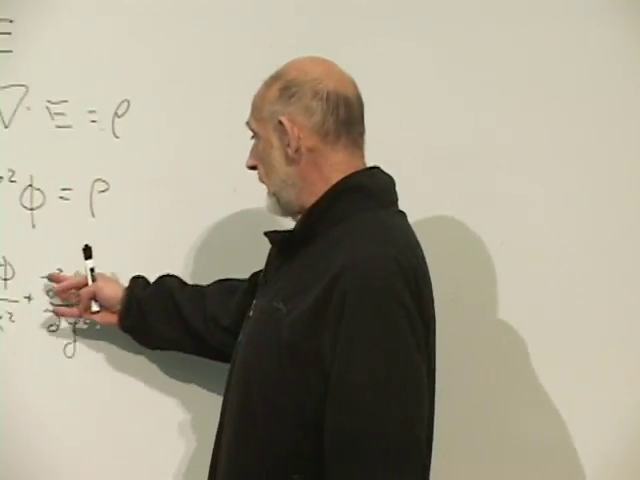
\includegraphics[width=0.70\textwidth]{lecture_08_figure_02.png}
  \caption{상대 부호가 마이너스인 것을 포함해 완성된 코시--리만 방정식 쌍.}
  \lectureframe{00:19:48}
  \label{fig:l08-cr-board}
\end{figure}

강의에서는 서로 연관된 용어를 간단히 구분한다. 유한 복소평면 전체에서 정칙인 함수는 전해석 함수다. 유리형 함수에는 고립된 극점이 있을 수 있다. 따라서 \(1/z\)는 \(z=0\)을 제외한 곳에서는 해석적이지만 전해석 함수는 아니다.

\section{조화 켤레와 등각 기하}

코시--리만 방정식은 결합된 1계 방정식이지만, 서로 분리된 2계 방정식을 함의한다. \(\partial_xu=\partial_yv\)를 \(x\)에 대해 미분하고, \(\partial_yu=-\partial_xv\)를 \(y\)에 대해 미분한 다음 더하면
\begin{align}
  \partial_x^2u&=\partial_x\partial_yv,\\
  \partial_y^2u&=-\partial_y\partial_xv,\\
  \therefore\qquad
  \partial_x^2u+\partial_y^2u&=0.
  \label{eq:l08-harmonic-u}
\end{align}
\(u\)와 \(v\)를 맞바꾸어 같은 논증을 반복하면
\begin{equation}
  \partial_x^2v+\partial_y^2v=0.
  \label{eq:l08-harmonic-v}
\end{equation}
따라서 해석 함수의 실수부와 허수부는 서로 조화 켤레다. 임의의 두 조화 함수가 자동으로 해석 함수를 이루는 것은 아니다. 두 함수는 여전히 \eqref{eq:l08-cauchy-riemann}로 연결되어야 한다.

\begin{figure}[H]
  \centering
  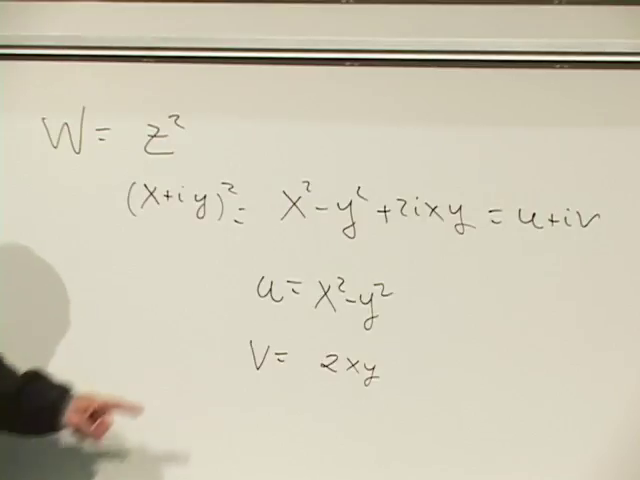
\includegraphics[width=0.68\textwidth]{lecture_08_figure_03.png}
  \caption{혼합 미분항이 상쇄되어 해석 사상의 한 성분에 대한 라플라스 방정식이 남는다.}
  \lectureframe{00:23:09}
  \label{fig:l08-harmonic-board}
\end{figure}

유용한 벡터 해석도 있다. \(\mathbf F=(u,-v)\)라면, 두 Cauchy--Riemann 방정식은 선택한 방향 규약에 따라 \(\mathbf F\)의 발산과 이차원 컬이 모두 사라짐을 나타낸다. 이것이 정전기학으로 돌아온다는 뜻이다.

\subsection{각도가 보존되는 이유}

두 개의 작은 복소 변위를 극형식으로 쓰자.
\begin{equation}
  \delta z=\rho e^{i\theta},
  \qquad
  \Delta z=\rho'e^{i\theta'}.
\end{equation}
두 변위의 비의 위상은 정확히 두 변위 사이의 각도인 \(\theta-\theta'\)이다. 해석 사상 아래에서는
\begin{equation}
  \frac{\delta w}{\delta z}
  =\frac{\Delta w}{\Delta z}
  =w'(z),
\end{equation}
미분 계수가 방향에 의존하지 않기 때문이다. 이를 정리하면
\begin{equation}
  \frac{\Delta z}{\delta z}
  =\frac{\Delta w}{\delta w}.
  \label{eq:l08-angle-ratio}
\end{equation}
양변의 위상이 같으므로 원래 선분 사이의 각도는 그 상 사이의 각도와 같다.

\begin{figure}[H]
  \centering
  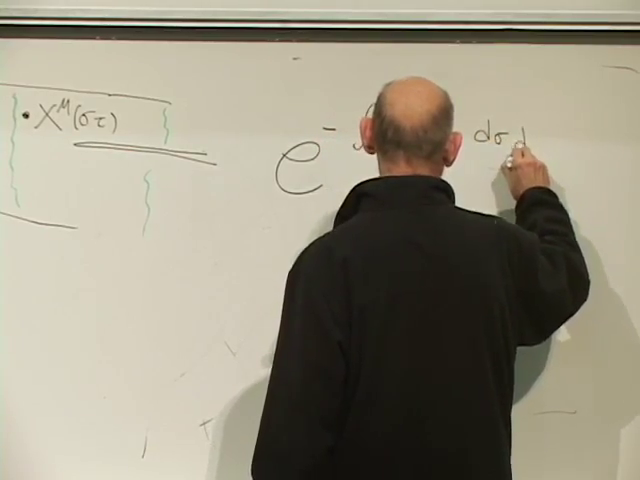
\includegraphics[width=0.70\textwidth]{lecture_08_figure_04.png}
  \medskip

  \begin{tikzpicture}[x=0.9cm,y=0.9cm,>=Latex]
    \begin{scope}
      \draw[->] (-0.2,0) -- (2.3,0);
      \draw[->] (0,-0.2) -- (0,2.1);
      \draw[very thick,blue!65!black,->] (0,0) -- (1.85,0.45)
        node[right] {\(\delta z\)};
      \draw[very thick,orange!75!black,->] (0,0) -- (0.72,1.65)
        node[above] {\(\Delta z\)};
      \draw (0.58,0.14) arc[start angle=14,end angle=66,radius=0.60];
      \node at (1.0,-0.55) {\(z\)-plane};
    \end{scope}
    \draw[->,thick] (3.0,0.9) -- (4.2,0.9)
      node[midway,above] {\(w(z)\)};
    \begin{scope}[xshift=5.0cm]
      \draw[->] (-0.2,0) -- (2.3,0);
      \draw[->] (0,-0.2) -- (0,2.1);
      \draw[very thick,blue!65!black,->] (0,0) -- (1.65,0.70)
        node[right] {\(\delta w\)};
      \draw[very thick,orange!75!black,->] (0,0) -- (0.48,1.62)
        node[above] {\(\Delta w\)};
      \draw (0.54,0.23) arc[start angle=23,end angle=74,radius=0.59];
      \node at (1.0,-0.55) {\(w\)-plane};
    \end{scope}
  \end{tikzpicture}
  \caption{칠판의 증명과 이를 국소적으로 깔끔하게 재구성한 그림. \(w'(z)\)를 곱하면 무한소 방향마다 같은 양만큼 회전하고 크기가 변하므로 방향 사이의 상대 각도가 보존된다.}
  \lectureframe{00:34:11}
  \label{fig:l08-angle-proof}
\end{figure}

이 국소 논증은 \(w'(z)\neq0\)을 가정한다. 임계점에서는 사상이 국소적으로 일대일이 아닐 수 있으므로 기하를 별도로 다루어야 한다. 그런 점을 제외하면 해석 사상과 방향을 보존하는 등각 사상은 국소적으로 같은 대상이다.

\section{눈에 익히기 위한 예제}

\subsection{제곱 사상과 복소켤레}

\(w=z^2\)일 때,
\begin{equation}
  (x+iy)^2=x^2-y^2+2ixy=u+iv,
\end{equation}
따라서
\begin{equation}
  u=x^2-y^2,
  \qquad
  v=2xy.
  \label{eq:l08-z-squared-components}
\end{equation}
\(u\)의 이계 도함수는 \(2\)와 \(-2\)이고, \(v\)의 이계 도함수들은 각각 사라진다. 두 함수 모두 조화 함수이며, 직접 미분해도 Cauchy--Riemann 방정식이 성립함을 확인할 수 있다.

\begin{figure}[H]
  \centering
  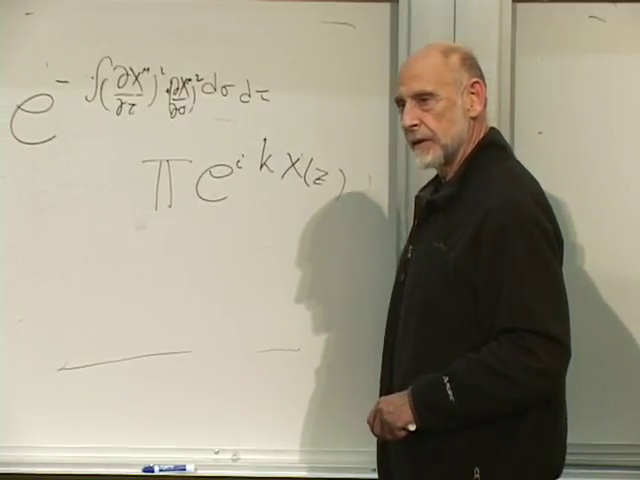
\includegraphics[width=0.72\textwidth]{lecture_08_figure_05.png}
  \caption{제곱 사상을 실수부와 허수부인 조화 성분으로 분해했다.}
  \lectureframe{00:36:45}
  \label{fig:l08-z-square-board}
\end{figure}

\begin{classroomqa}
\audiencequestion{\(1/z\)는 비해석 함수의 예인가요?
\lecturetimestamp{00:37:49}}
\lecturerresponse{한 점에서만 그렇다. \(z\neq0\)인 곳에서는 해석적이며 원점에 극점이 있다. 어디에서나 코시--리만 판정에 실패하는 사상을 보려면 복소켤레가 더 나은 예다.}
\end{classroomqa}

반면,
\begin{equation}
  w=\bar z=x-iy
  \qquad\Longrightarrow\qquad
  u=x,\quad v=-y
\end{equation}
이 사상은 방향을 뒤집는다. 그 도함수는 첫 번째 코시--리만 방정식에서 부호가 맞지 않으므로 \(z\)의 함수로서 해석적이지 않다.

\begin{figure}[H]
  \centering
  \includegraphics[width=0.62\textwidth]{lecture_08_figure_06.png}
  \caption{일부러 비해석적인 반례로 든 복소켤레.}
  \lectureframe{00:38:38}
  \label{fig:l08-conjugate-board}
\end{figure}

\subsection{지수 함수와 그 역함수}

\begin{classroomqa}
\audiencequestion{\(e^z\)가 해석 함수라면 그 역함수 \(\log z\)도 해석적이어야 하는 이유는 무엇인가요? \lecturetimestamp{00:40:38}}
\lecturerresponse{역함수가 존재하고 \(w'(z)\neq0\)인 곳에서는 그 도함수가 \(1/w'(z)\)이다. 따라서 방향 독립성이 보존된다. 로그 함수는 전역적으로 다가 함수이므로 가지를 하나 택하고 분기점과 분지선을 제외한다. 그 선택한 영역에서는 국소 등각 사상이 여전히 성립한다.}
\end{classroomqa}

오일러 공식으로부터
\begin{equation}
  w=e^z=e^{x+iy}
  =e^x(\cos y+i\sin y),
\end{equation}
따라서
\begin{equation}
  u=e^x\cos y,
  \qquad
  v=e^x\sin y.
  \label{eq:l08-exponential-components}
\end{equation}
예를 들어 \(\partial_xu=e^x\cos y=\partial_yv\)이고, 두 번째 코시--리만 방정식도 똑같이 직접 확인된다.

\begin{figure}[H]
  \centering
  \includegraphics[width=0.68\textwidth]{lecture_08_figure_07.png}
  \caption{지수 사상의 실수부와 허수부.}
  \lectureframe{00:42:23}
  \label{fig:l08-exponential-board}
\end{figure}

\section{반평면, 띠, 원통, 원판}

\subsection{로그 함수는 반지름을 시간으로 바꾼다}

다음과 같은 오른쪽 반평면을 취하고,
\(-\pi/2<\theta<\pi/2\)
다음과 같이 쓰자.
\begin{equation}
  z=re^{i\theta},
  \qquad
  w=\log z=\log r+i\theta.
  \label{eq:l08-log-map}
\end{equation}
이 반평면은 무한한 띠로 사상된다.
\begin{equation}
  -\frac{\pi}{2}<\operatorname{Im}w<\frac{\pi}{2}.
\end{equation}
\(\theta\)가 일정한 반직선은 수평선이 되고, \(r\)가 일정한 반원은 수직선이 된다. 원점은 \(\operatorname{Re}w=-\infty\)으로 사상되고, \(r=\infty\)는 \(\operatorname{Re}w=+\infty\)으로 사상된다.

\begin{figure}[H]
  \centering
  \includegraphics[width=0.75\textwidth]{lecture_08_figure_08.png}
  \caption{로그 함수는 오른쪽 반평면을 무한한 띠로 보낸다. 극좌표의 반직선과 반원은 직교하는 직사각형 격자가 된다.}
  \lectureframe{00:47:48}
  \label{fig:l08-log-strip-board}
\end{figure}

띠는 열린 끈의 표준 세계면이다. 띠의 유계 좌표는 끈을 따라가는 매개변수이고, 무한히 뻗은 방향으로의 평행 이동은 세계면 시간이다. 역 지수 사상 아래에서는 시간 평행 이동이 확대 \(z\mapsto e^a z\)로 바뀐다. 따라서 같은 대칭이 띠에서는 평행 이동으로, 반평면에서는 균일한 팽창으로 나타난다.

\begin{classroomqa}
\audiencequestion{\(r=1\) 같은 특정한 값은 어디로 가며, 띠의 좌표는 여전히 극좌표인가요? \lecturetimestamp{00:50:58}}
\lecturerresponse{반지름이 일정한 원은 \(\operatorname{Re}w=\log r\)에서 수직선이 된다. 특히 \(r=1\)는 중심선 \(\operatorname{Re}w=0\)로 사상된다. 극좌표는 \(z\)평면을 나타낸다. \(w\)평면에서는 보통의 직교 좌표를 사용한다. \((\log r,\theta)\)}
\end{classroomqa}

천공된 평면 전체에 \(\log z\)를 적용하면 각 좌표의 주기는 \(2\pi\)이다. 따라서 결과인 띠의 위쪽과 아래쪽 가장자리는 서로 동일시되어 무한 원통이 된다. 경계가 있는 반평면은 열린 끈의 세계면을 나타낸다. 경계가 없고 각도가 주기적인 전체 평면은 닫힌 끈의 원통을 나타낸다.

\begin{figure}[H]
  \centering
  \includegraphics[width=0.75\textwidth]{lecture_08_figure_09.png}
  \caption{반평면과 띠의 모습, 그리고 천공된 평면 전체를 닫힌 끈의 원통으로 만드는 주기적 동일시.}
  \lectureframe{00:54:23}
  \label{fig:l08-open-closed-board}
\end{figure}

\subsection{단위원판으로 보내는 케일리 사상}

선형 분수 사상, 즉 뫼비우스 사상은 오른쪽 반평면을 단위원판으로 보낸다.
\begin{equation}
  w=\frac{z-1}{z+1}.
  \label{eq:l08-cayley}
\end{equation}
이 사상은 \(z=0\)를 \(-1\)로, \(z=\infty\)를 \(+1\)으로 보내고, 허수축은 \(|w|=1\)로 보낸다. \(z=ir\)이면
\begin{equation}
  \left|\frac{ir-1}{ir+1}\right|=1.
\end{equation}
\(\operatorname{Re}z>0\)인 점들은 원판 안에 놓이며, 왼쪽 반평면은 원판 바깥으로 사상된다.
\editorialnote{강의 중 유도에서는 원판 내부로 사상된다고 설명하면서 역수 \((z+1)/(z-1)\)를 쓴다. 이 역수도 단위원 경계를 갖지만 오른쪽 반평면을 외부로 보낸다. 식 \eqref{eq:l08-cayley}은 설명한 기하와 일치하는 원판 내부 사상 규약이다.}

\begin{figure}[H]
  \centering
  \includegraphics[width=0.72\textwidth]{lecture_08_figure_10.png}
  \caption{단위원 경계를 만드는 선형 분수 사상. 칠판에 나타난 역수 규약은 원판 내부와 외부를 맞바꾼다.}
  \lectureframe{00:58:38}
  \label{fig:l08-cayley-board}
\end{figure}

뫼비우스 사상은 원과 직선으로 이루어진 일반화된 모임을 원과 직선으로 보낸다. 따라서 반평면의 반지름 방향 격자와 원형 격자는 원판 안의 서로 직교하는 두 호의 집합이 된다. 직선 지름은 중심이 무한대로 간 원의 극한에 해당한다.

\begin{classroomqa}
\audiencequestion{원판 안에 그린 곡선들은 정말 원인가요?
\lecturetimestamp{01:00:55}}
\lecturerresponse{그렇다. 원의 중심은 서로 다른 위치에 있으며, 그중에는 눈에 보이는 원판 바깥에 있는 것도 많다. 지름은 같은 원 집합에서 반지름이 무한대가 되는 극한이다.}
\end{classroomqa}

\begin{classroomqa}
\audiencequestion{원판 그림은 이것이 구면이라는 뜻인가요? 다른 반평면은 어디로 가나요? \lecturetimestamp{01:01:21}}
\lecturerresponse{여기 그림은 구면이 아니라 평평한 원판이다. 오른쪽 반평면은 원판 경계 안으로 사상되고 왼쪽 반평면은 바깥으로 사상된다. 복소평면 전체에 무한대점을 더하면, 확장된 평면을 입체 사영으로 구면에 나타낼 수 있다. 이는 전역적인 성질에 관한 별개의 진술이다.}
\end{classroomqa}

\begin{classroomqa}
\audiencequestion{원래의 방사형 선들과 반지름이 일정한 반원은 원판의 어떤 곡선에 대응하나요? \lecturetimestamp{01:02:59}}
\lecturerresponse{양의 실수축은 \(-1\)와 \(+1\)를 잇는 지름이 된다. 다른 반직선들도 같은 두 경계점을 잇는 원호가 된다. 반지름이 일정한 반원은 단위원에서 시작해 단위원에서 끝나는 직교 곡선 집합이 된다.}
\end{classroomqa}

\begin{figure}[H]
  \centering
  \includegraphics[width=0.72\textwidth]{lecture_08_figure_11.png}
  \caption{반평면의 직선과 반원은 원판 안에서 서로 직교하는 원과 직선의 집합으로 바뀐다.}
  \lectureframe{01:03:48}
  \label{fig:l08-circle-grid-board}
\end{figure}

\section{네 끈 세계면}

이제 산란으로 돌아가자. 열린 끈 두 개가 들어와 하나로 합쳐지고, 임의의 시간 동안 전파된 다음, 나가는 끈 두 개로 갈라진다. 띠 좌표에서 세계면은 양 끝에서 절개한 긴 띠처럼 보인다---이른바 ‘스포츠 밴드’ 그림이다. 중간 끈의 수명은 미리 정해져 있지 않다. 산란 진폭을 적분할 때 포함되는 여러 이력 중 하나다.

\((\sigma,\tau)\)를 세계면 좌표라고 하고,
\begin{equation}
  X^\mu=X^\mu(\sigma,\tau)
  \label{eq:l08-embedding}
\end{equation}
이 좌표가 시공간에서의 위치를 나타낸다고 하자. \(\sigma,\tau\)라는 표지는 2차원 매개변수 곡면에 속하고, 지표 \(\mu\)는 시공간 좌표를 나타낸다. 보손 이론에서는 \(\mu=0,\ldots,25\)이며, 초끈의 경우에는 시공간 좌표가 10개다.

위크 회전 뒤 자유 매장장의 유클리드 작용은 다음과 같다.
\begin{equation}
  S_E[X]
  =\frac{1}{4\pi\alpha'}\int_\Sigma d\sigma\,d\tau\,
  \left[
    \partial_\tau X^\mu\partial_\tau X_\mu
    +\partial_\sigma X^\mu\partial_\sigma X_\mu
  \right].
  \label{eq:l08-euclidean-action}
\end{equation}
이에 대응하는 경로 적분은 선택한 세계면을 시공간에 매장하는 모든 경우를 합한다.
\begin{equation}
  \int\mathcal D X\,e^{-S_E[X]}.
  \label{eq:l08-bare-worldsheet-integral}
\end{equation}

\begin{figure}[H]
  \centering
  \includegraphics[width=0.74\textwidth]{lecture_08_figure_12.png}
  \caption{완성된 양의 유클리드 세계면 가중치. 두 미분항은 모든 시공간 성분에 대해 합산한다.}
  \lectureframe{01:11:34}
  \label{fig:l08-action-board}
\end{figure}

절개된 띠에는 연결된 경계가 하나 있다. 따라서 등각 자유도를 이용해 이를 원판으로 나타낼 수 있다. 띠의 멀리 떨어진 네 끝은 경계 위의 네 표시점이 된다. 표시점의 위치를 변형하면 띠 좌표에서 합쳐짐과 분리 사이의 겉보기 간격은 달라지지만, 바탕이 되는 곡면이나 물리는 바뀌지 않는다.

\begin{figure}[H]
  \centering
  \includegraphics[width=0.76\textwidth]{lecture_08_figure_13.png}
  \caption{절개된 띠 세계면과 외부 끈의 경계점 네 개를 표시한 원판 표현.}
  \lectureframe{01:15:18}
  \label{fig:l08-bandage-disc-board}
\end{figure}

이 등각 사상을 그림으로 나타낼 때 쓰는 세부 격자선에는 물리적 의미가 없다. 중요한 것은 위상, 경계, 그리고 표시된 외부점이다. 같은 세계면을 서로 다른 채널의 모습으로 늘여 그릴 수 있지만, 새로운 상호작용이 생기는 것은 아니다.

\section{외부 상태를 경계 삽입으로 나타내기}

기본 적분 \eqref{eq:l08-bare-worldsheet-integral}만으로는 어떤 운동량이 들어오고 나가는지 알 수 없다. 운동량 \(k_i^\mu\)를 가진 스칼라 열린 끈 상태에 대해 경계에 다음 꼭짓점 연산자를 삽입하자.
\begin{equation}
  V_i(z_i)=e^{\,i k_i\cdot X(z_i)},
  \qquad
  k_i\cdot X=k_{i\mu}X^\mu.
  \label{eq:l08-vertex}
\end{equation}
점 \(z_i\)는 세계면 경계 위의 위치다. 시공간 좌표도, 운동량 방향도 아니다.

\begin{figure}[H]
  \centering
  \includegraphics[width=0.72\textwidth]{lecture_08_figure_14.png}
  \caption{부피 내부의 유클리드 가중치와 경계의 운동량 삽입 곱을 서로 구별되는 인자로 나타냈다.}
  \lectureframe{01:18:58}
  \label{fig:l08-vertex-board}
\end{figure}

\(n\)개의 외부 열린 끈에 대해 개략적인 처방은 다음과 같다.
\begin{equation}
  \begin{aligned}
    \mathcal A_n(k_1,\ldots,k_n)
    &=\int_{\mathcal M_{0,n}^{\partial}}\!d\mu(z_i)
      \int\mathcal D X\\
    &\quad\times e^{-S_E[X]}
      \prod_{i=1}^{n}e^{\,i k_i\cdot X(z_i)}.
  \end{aligned}
  \label{eq:l08-open-string-prescription}
\end{equation}
함수 적분은 매장 \(X^\mu\)에 대해 수행한다. 유한 차원 적분은 서로 동등하지 않은 경계 삽입 위치에 대해 수행한다. 강의에서와 같이 이 단계에서는 편극 인자와 게이지 고정 측도를 생략했다.
\editorialnote{완전한 게이지 고정 끈 진폭에는 적절한 고스트 기여, 상태에 따른 꼭짓점 인자, 결합 상수, 정규화도 들어간다. 식 \eqref{eq:l08-open-string-prescription}은 이 강의에서 다룬 매장장과 위치의 의존성을 나타낸다.}

\begin{classroomqa}
\audiencequestion{외부 운동량이 고정되어 있다면 왜 그 운동량에 대해 적분하나요? \lecturetimestamp{01:20:42}}
\lecturerresponse{운동량에 대해서는 적분하지 않는다. \(k_i\)는 산란 진폭의 고정된 표지다. 적분하는 것은 매장장과, 고정된 운동량이 삽입되는 세계면 위치 \(z_i\)다. 후자의 적분은 띠 그림에서 중간 끈의 수명에 대한 적분을 대신한다.}
\end{classroomqa}

\begin{classroomqa}
\audiencequestion{꼭짓점 인자의 곱은 경로 적분 안에 들어가나요? 작용의 일부인가요? \lecturetimestamp{01:21:39}}
\lecturerresponse{그 곱은 함수 적분 안에서 \(e^{-S_E}\)에 곱해진다. 인자들을 지수화해 작용에 국소화된 원천항을 더한 것으로 보아도 되지만, 개념적으로 이들은 자유 부피 작용의 일부가 아니라 꼭짓점 연산자다.}
\end{classroomqa}

\begin{figure}[H]
  \centering
  \includegraphics[width=0.76\textwidth]{lecture_08_figure_15.png}
  \caption{연속하는 외부 입자에 대한 인자 \(e^{ik_i\cdot X(z_i)}\)를 각각 따로 둔 경로 적분.}
  \lectureframe{01:23:23}
  \label{fig:l08-full-prescription-board}
\end{figure}

\begin{classroomqa}
\audiencequestion{세계면을 위크 회전한 뒤에도 \(e^{ik\cdot X}\)에 \(i\)가 남아 있는 이유는 무엇인가요? \lecturetimestamp{01:23:42}}
\lecturerresponse{회전은 세계면 시간을 바꾸며 부피 가중치를 \(e^{iS}\)에서 \(e^{-S_E}\)으로 바꾼다. 운동량 고유함수에 들어 있는 \(i\)는 시공간 운동량을 나타내는 푸리에 위상이다. 그 역할은 다르므로 그대로 남는다.}
\end{classroomqa}

\begin{classroomqa}
\audiencequestion{위치 \(z_i\)가 운동량 벡터의 방향을 정하나요? \lecturetimestamp{01:24:19}}
\lecturerresponse{아니다. 방향은 시공간 성분 \(k_i^\mu\)에 담긴다. 삽입점 \(z_i\)는 그 운동량이 세계면 기술에 어디에 들어가는지를 나타낸다. \(X^\mu(z_i)\)는 \(\mathcal D X\)에서 적분하는 장의 값들 중 하나다.}
\end{classroomqa}

\begin{classroomqa}
\audiencequestion{밴드 다리의 그림에서 보이는 각도가 물리적 운동량의 방향을 나타내나요? \lecturetimestamp{01:25:07}}
\lecturerresponse{아니다. 밴드는 매개변수 공간이지, 물리적 시공간에서 끈의 모습을 나타낸 그림이 아니다. 다리는 수평이나 기울어진 방향으로 그릴 수도 있고, 등각적으로 휘어 그릴 수도 있다. 물리적 방향은 성분 \(k^\mu\)으로 표현되고, \(X^\mu(\sigma,\tau)\)는 적분 변수다.}
\end{classroomqa}

\section{정전기학으로 보는 가우스 적분}

작용 \eqref{eq:l08-euclidean-action}은 모든 \(X^\mu\) 성분에 대해 이차식이고, 삽입항의 지수들을 작용과 결합하면 이 삽입항들은 선형 원천이 된다. 따라서 함수 적분은 가우스 적분이다. 안장점에서 각 시공간 성분은 다음과 같은 개략적인 푸아송 방정식을 만족한다.
\begin{equation}
  \nabla^2 X^\mu(z)
  \propto
  i\alpha'\sum_i k_i^\mu\,\delta(z-z_i),
  \label{eq:l08-electrostatic-source}
\end{equation}
원판 가장자리에서는 열린 끈 경계 조건을 적용한다. 각 \(X^\mu\)는 서로 독립인 정전기 퍼텐셜처럼 작용하고, 각 운동량 성분 \(k_i^\mu\)은 위치 \(z_i\)에 놓인 이에 대응하는 전하처럼 작용한다.

\begin{figure}[H]
  \centering
  \includegraphics[width=0.76\textwidth]{lecture_08_figure_16.png}
  \caption{경계 원천이 있는 원판을 시공간 성분마다 독립적인 2차원 정전기 문제 하나로 해석한다.}
  \lectureframe{01:28:58}
  \label{fig:l08-electrostatic-disc-board}
\end{figure}

정전기 문제를 풀고, 그 에너지를 계산하고, 음의 에너지를 지수화한 다음, 서로 동등하지 않은 전하 위치에 대해 적분한다. 표준 열린 끈 정규화에서 매장장 상관함수는 코바--닐센 인자를 준다.
\begin{equation}
  \left\langle\prod_i e^{\,ik_i\cdot X(z_i)}\right\rangle
  \propto
  (2\pi)^D\delta^{(D)}\!\left(\sum_i k_i\right)
  \prod_{i<j}|z_i-z_j|^{2\alpha' k_i\cdot k_j}.
  \label{eq:l08-koba-nielsen}
\end{equation}
델타 함수는 운동량 보존을 나타낸다. 곱에는 전하 사이의 정전기적 쌍 에너지가 들어 있다. 여기서 다루는 스칼라 경계 삽입 네 개의 경우, 위치 세 개를 고정하면 남은 적분은 앞선 강의에서 다룬 오일러 베타 적분이 된다.

\begin{classroomqa}
\audiencequestion{정전기 에너지는 26개인가요, 아니면 하나뿐인가요?
\lecturetimestamp{01:30:53}}
\lecturerresponse{시공간 성분마다 서로 독립적인 퍼텐셜과 장이 하나씩 있다. 정규 직교 표적공간 기저에서는 이들의 이차 에너지 사이에 교차항이 없으며, 지수화하기 전에 기여분들을 하나의 전체 작용에 더한다.}
\end{classroomqa}

\begin{classroomqa}
\audiencequestion{원판의 각 좌표는 물리적 산란각인가요? \lecturetimestamp{01:32:10}}
\lecturerresponse{아니다. 세계면 위치를 나타내는 매개변수다. 서로 동등하지 않은 위치의 조합은 중간 전파 구간과 관련되며 적분된다. 물리적 산란각은 고정된 운동량으로 만든 로런츠 불변량에 담긴다.}
\end{classroomqa}

\begin{classroomqa}
\audiencequestion{임계 차원에서 벗어나면 이 구성이 성립하지 않는 이유는 무엇인가요? \lecturetimestamp{01:32:35}}
\lecturerresponse{형식적인 가우스 적분만으로 일관성 조건을 모두 만족하는 것은 아니다. 게이지 고정은 등각 이상을 도입하며, 물질과 고스트의 기여는 임계 차원에서만 상쇄된다. 보손 끈에서는 \(D=26\)이고 초끈에서는 \(D=10\)이다. 이 상쇄가 없으면 양자 세계면의 등각 대칭이 사라진다.}
\end{classroomqa}

\begin{classroomqa}
\audiencequestion{이미 큰 공간 차원 세 개와 콤팩트한 여분 차원을 가정한 건가요? \lecturetimestamp{01:33:38}}
\lecturerresponse{아니다. 아직 콤팩트화는 이 구성에 들어오지 않았다. 이 단계에서 보손 좌표는 여전히 표적공간의 26개 방향 전체를, 초끈의 경우에는 10개 방향 전체를 누빈다. 그중 일부가 거시적으로 큰 상태로 남을 수 있는 방법은 다음 논의에서 다룬다.}
\end{classroomqa}

\begin{classroomqa}
\audiencequestion{정전기학과의 연관성은 좌표가 라플라스 방정식을 만족한다는 점뿐인가요? \lecturetimestamp{01:33:57}}
\lecturerresponse{그렇다. 삽입점에서 떨어진 곳에서는 각 \(X^\mu\)가 조화 함수이고, 꼭짓점 연산자는 델타 함수 원천을 제공한다. 정전기학 용어를 사용하든 말든, 이는 점전하가 있는 정적인 2차원 퍼텐셜의 경계값 문제와 수학적으로 동일하다.}
\end{classroomqa}

\subsection{등각 중복성과 모듈라이의 개수}

원판에는 3개의 실수 매개변수로 이루어진 등각 자기동형군 \(\mathrm{PSL}(2,\mathbb R)\)이 있다. 따라서 순서가 정해진 경계점 세 개를 편리한 위치에 고정할 수 있다. 외부 끈 네 개의 경우에는 네 번째 위치만 적분 대상으로 남는다. 순서가 정해진 경계 삽입이 \(n\)개라면 나무 수준에서 남는 실수 위치 적분은
\begin{equation}
  n-3
  \label{eq:l08-n-minus-three}
\end{equation}
개다.

\begin{classroomqa}
\audiencequestion{원판 둘레의 각 위치 네 개는 서로 독립인가요? \lecturetimestamp{01:34:37}}
\lecturerresponse{물리적으로는 그렇지 않다. 처음에는 위치 네 개를 쓰지만 원판의 등각 대칭으로 그중 아무 세 개나 원하는 위치에 둘 수 있다. 두 끈이 들어오고 두 끈이 나가는 진폭에서는 네 번째 위치의 상대적 위치만 남는다.}
\end{classroomqa}

\begin{figure}[H]
  \centering
  \includegraphics[width=0.72\textwidth]{lecture_08_figure_17.png}
  \caption{원판 경계의 삽입 네 개. 등각 자유도로 임의의 세 개를 고정하면 네 점 진폭의 모듈러스 하나가 남는다.}
  \lectureframe{01:35:18}
  \label{fig:l08-fix-three-board}
\end{figure}

\begin{classroomqa}
\audiencequestion{띠 그림에서 두 분리점이 같은 높이에 있지 않으면 어떻게 되나요? \lecturetimestamp{01:35:24}}
\lecturerresponse{등각 사상으로 겉보기의 높이 차이를 없앨 수 있다. 서로 다른 그림은 같은 모듈러스를 나타내는 좌표 표현이다. 불변인 적분은 남은 경계 위치, 또는 그와 동등하게 전파 구간에 대한 적분이다.}
\end{classroomqa}

\begin{classroomqa}
\audiencequestion{외부 입자가 더 많으면 위치 매개변수는 몇 개 남나요? \lecturetimestamp{01:36:00}}
\lecturerresponse{등각 대칭으로 삽입점 세 개를 고정하고 나머지 \(n-3\)개를 적분한다. 이것이 순서가 정해진 나무 수준 열린 끈 진폭에서 경계 모듈라이의 개수다.}
\end{classroomqa}

\begin{classroomqa}
\audiencequestion{이것은 M이론과 어떤 관계가 있나요?
\lecturetimestamp{01:36:37}}
\lecturerresponse{아직은 없다. 여기서 다룬 구성은 세계면 위의 섭동적 열린 끈 산란이다. M이론과의 관계에는 이후의 쌍대성과 비섭동적 개념이 필요하므로, 이 질문은 뒤로 미룬다.}
\end{classroomqa}

\begin{classroomqa}
\audiencequestion{수직 방향의 띠 그림이나 교차된 띠 그림은 서로 다른 계산을 뜻합니까? \lecturetimestamp{01:36:49}}
\lecturerresponse{아닙니다. 편리한 한 점을 고정하고 나머지 모듈러스가 전체 구간을 훑도록 둘 수 있습니다. 띠 그림과 원판 위 경계점 적분은 같은 적분을 서로 다르게 절단해 나타낸 것이며, 따라서 모든 외부 끈을 대칭적으로 다룰 수 있습니다.}
\end{classroomqa}

\section{처방으로 아직 해결되지 않는 문제}

원판 공식은 외부 끈이 더 많은 경우에도 즉시 확장됩니다. 꼭짓점 연산자를 더하고, 서로 동등하지 않은 경계 위치 \(n-3\)개에 대해 적분하면 됩니다. 이는 일관된 끈 모형을 위한 정밀한 나무 수준 처방이지만, 관측된 입자 물리학을 현실적으로 기술하는 모형은 아직 아닙니다. 단순한 보손 이론은 시공간 차원이 맞지 않고 다른 물리적 결함도 있습니다. 초끈 이론은 스펙트럼을 개선하고 임계 차원을 10으로 낮추지만, 여전히 6개의 공간 차원을 콤팩트화해야 합니다.

\begin{classroomqa}
\audiencequestion{이 단순한 모형은 입자 충돌 실험과 이미 일치합니까? \lecturetimestamp{01:39:06}}
\lecturerresponse{아닙니다. 공명 구조는 역사적으로 강입자 산란과 비슷했지만, 26차원 보손 모형은 관측된 입자를 직접 기술할 수 없습니다. 형식론은 이 모형의 산란 진폭을 정의합니다. 자연과 일치시키려면 현실적인 스펙트럼, 콤팩트화, 상호작용, 진공 선택이 필요합니다.}
\end{classroomqa}

\begin{classroomqa}
\audiencequestion{콤팩트화하면 여분의 차원이 줄어들고 현실적인 입자 데이터가 나옵니까? \lecturetimestamp{01:41:10}}
\lecturerresponse{거시적으로 유효한 차원을 줄이고 입자 스펙트럼과 게이지 군을 만들어 낼 수 있습니다. 수학적으로 어려운 문제의 상당 부분도 바로 여기서 시작됩니다. 일관된 콤팩트화는 많이 알려져 있지만, 관측된 기본 입자를 기술하는 유일한 모형을 선택하는 문제는 아직 해결되지 않았습니다.}
\end{classroomqa}

이 강의는 완성된 이론을 내세우기보다 이 차이를 강조합니다. 끈 이론의 구성은 수학적으로 명확하며 중력과 기하학에 관한 깊은 정보를 밝혀 왔지만, 그 구성의 다양성 자체가 물리학의 문제이기도 합니다.

\begin{classroomqa}
\audiencequestion{보손 끈 이론의 임계 차원이 26인 이유를 간단히 기억할 방법이 있습니까? \lecturetimestamp{01:43:19}}
\lecturerresponse{앞서 진동자 계산에서는 정규화된 영점 에너지 합 \(1+2+3+\cdots=-1/12\)을 사용했습니다. 횡방향 진동자의 기여에는 24개의 방향이 들어가며, 종방향 시공간 좌표 2개를 다시 포함하면 \(24+2=26\)가 됩니다. 이는 앞서 제시한 일관성 논증을 기억하기 위한 요령이지, 여기서 새로 유도하는 것은 아닙니다.}
\end{classroomqa}

\begin{classroomqa}
\audiencequestion{삽입된 운동량 벡터 \(k_i\) 자체도 양자화됩니까?
\lecturetimestamp{01:43:46}}
\lecturerresponse{비콤팩트 시공간에서는 운동량 벡터의 성분이 연속적입니다. 양자화되는 것은 진동자 준위이며, 따라서 허용되는 질량 제곱 스펙트럼이 양자화됩니다. 콤팩트 차원에서는 그에 대응하는 운동량 성분과 감김 성분이 양자화될 수 있지만, 그것은 다음 논의에서 다룹니다.}
\end{classroomqa}

\chapter{끈, 중력, 콤팩트화와 T-쌍대성}

\lectureoverview{점입자는 거의 모든 매끄러운 기하 위에서 일관되게 운동할 수 있지만, 양자 끈은 그렇지 않다. 끈의 무한히 많은 영점 진동은 표적 공간을 점점 더 짧은 길이 척도에서 탐사하며, 그 진동들을 다시 포함할수록 유효 기하가 변한다. 이 과정에 고정점이 존재하도록 요구하면 \(R_{\mu\nu}=0\), 즉 진공 아인슈타인 방정식을 얻는다. 이어서 이 일관성 조건에서 콤팩트화로 넘어간다. 원은 칼루차--클라인 운동량 상태와 끈 감김 상태를 모두 제공한다. 두 상태를 서로 바꾸면 반지름이 \(R\)인 원과 반지름이 \(\alpha'/R\)인 원이 서로 대응한다.}

\section{선택 원리로서의 일관성}

답해야 할 질문은 두 가지다. 왜 끈 이론에는 중력이 나타나며, 끈 이론은 왜 점입자 역학보다 허용되는 배경이 훨씬 제한적인가? 사실 이 둘은 같은 질문이다. 배경 기하는 끈을 얼마나 세밀하게 분해하는지에 임의로 의존하지 않고 끈이 그 위에서 전파될 수 있을 때만 허용된다.

먼저 제어 사례를 살펴보자. 매끄러운 곡면 위에 구속된 점입자다. 고전적으로 입자는 곡면 위의 내재적인 직선에 해당하는 측지선을 따라간다. 운동을 짧은 선분 여러 개로 근사하고, 차분 방정식을 쓴 다음 선분 길이를 0으로 보내면 된다. 그 결과 연속극한이 잘 정의된 상미분방정식을 얻는다.

양자역학은 결론이 아니라 역사들의 합을 바꾼다. 하나의 고전적 경로를 선택하는 대신 곡면 위의 경로들에 대한 진폭을 합한다. 시간은 다시 작은 단계들로 나눌 수 있으며, 그 극한은 곡률이 있는 구성 공간에서의 Schr\"odinger 방정식으로 동등하게 기술된다. 곡면이 매끄러우면 극한은 확정된 전파자와 스펙트럼으로 수렴한다.

\begin{figure}[H]\centering
  \includegraphics[width=0.72\textwidth]{lecture_09_figure_01.png}\caption{곡면 위의 매끄러운 경로와 시간 분할 양자 합에서 나타나는 들쭉날쭉한 경로. 둘 다 표적 곡면에 내재되어 있다.}\lectureframe{00:05:10}\label{fig:l09-particle-paths}\end{figure}

\begin{classroomqa}\audiencequestion{경로 적분에서 모든 경로는 곡면 안에 머물러야 하나요? \lecturetimestamp{00:05:39}}\lecturerresponse{그렇다. 곡면은 입자의 구성 공간이지, 입자가 지름길로 가로지를 수 있도록 더 큰 공간에 끼워 넣은 막이 아니다. 중간의 모든 점은 곡면에 속하며, 모든 길이와 작용은 그 곡면의 내재적 계량으로 계산한다.}\end{classroomqa}

끈에 해당하는 질문은 더 어렵다. 끈은 질량중심 위치만으로 규정되지 않는다. 끈에는 무한한 진동자 탑이 있으므로, 분해능을 높인다는 것은 더 많은 동역학적 자유도를 허용한다는 뜻이다. 그 탑을 다시 포함할 때 관측량이 극한에 도달해야 이론이 일관성을 갖는다.

\section{구면 위의 점입자}

구면은 곡률이 있는 기하를 살펴보는 가장 단순한 시험 사례다. 반지름을 \(R\)라 하고, 먼저 질량 \(m\)인 입자를 그 위에 놓자. 대원을 따라 운동할 때는
\begin{equation}
  E=\frac{1}{2}mv^2=\frac{p^2}{2m},
  \qquad
  L=pR.
  \label{eq:l09-particle-energy}
\end{equation}
따라서
\begin{equation}
  E=\frac{L^2}{2mR^2}
   =\frac{L^2}{2I},
  \qquad
  I=mR^2.
  \label{eq:l09-rotor-energy}
\end{equation}
반지름은 관성 모멘트를 통해 들어간다. 각운동량을 양자화하면 익숙한 강체 회전자 스펙트럼이 나오며, 자외선 절단값에는 아무것도 의존하지 않는다.

\begin{figure}[H]\centering
  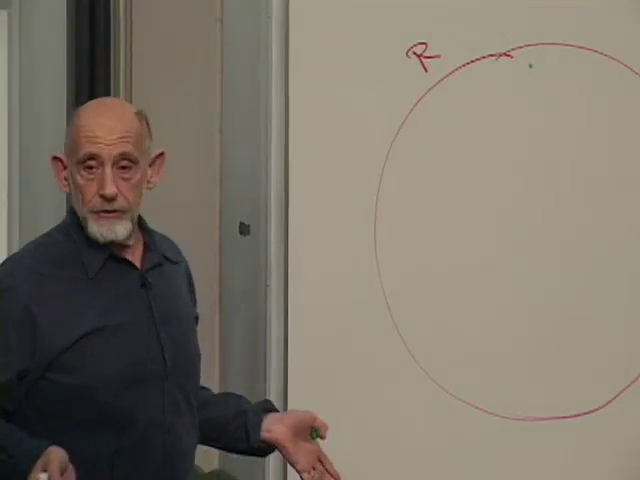
\includegraphics[width=0.74\textwidth]{lecture_09_figure_02.png}\caption{점입자 제어 계산:
\(p^2/(2m)=L^2/(2mR^2)=L^2/(2I)\).}\lectureframe{00:11:25}\label{fig:l09-sphere-rotor}\end{figure}

이처럼 문제가 없는 사례는 중요하다. 곡률 자체가 문제는 아니다. 문제는 곡률이 끈의 내부적인 양자적 크기와 결합할 때 나타난다.

\section{진공 상태의 끈은 점입자가 아니다}

열린 끈의 횡방향 좌표 하나를 생각하고 질량중심 성분을 빼자. 여기서 사용하는 진동자 전개는 개략적인 형태다:
\begin{equation}
  X(\sigma)-X_{\mathrm{cm}}
  \sim
  \sum_{n=1}^{\infty}
  \frac{a_n+a_n^\dagger}{\sqrt n}\cos(n\sigma).
  \label{eq:l09-mode-expansion}
\end{equation}
핵심 요소는 코사인 모드, 진동자 연산자, 그리고 \(1/\sqrt n\) 인자다. 크기 추정에는 정확한 정규화가 중요하지 않다.
\editorialnote{정확한 전개식에는 규약에 따라 달라지는 \(\alpha'\) 인자와 수치 상수, 그리고 진동자 표기법의 선택이 들어간다. 식 \eqref{eq:l09-mode-expansion}은 칠판에서 유도한 것과 마찬가지로 자외선 추정에 필요한 의존성만 남긴다.}

\begin{figure}[H]\centering
  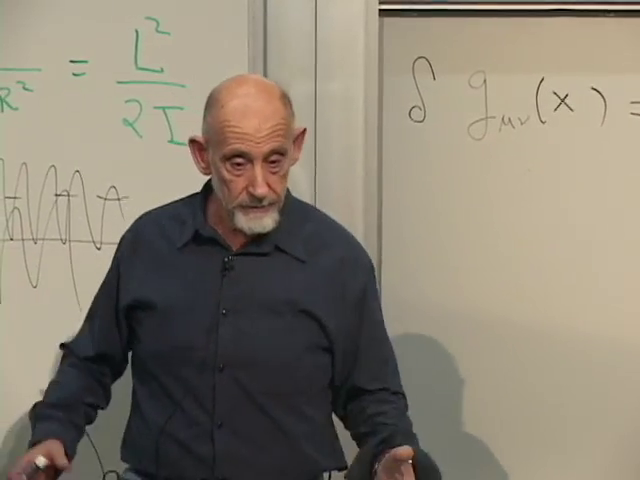
\includegraphics[width=0.78\textwidth]{lecture_09_figure_03.png}\caption{구조를 보여 주는 진동자 전개식과 이를 제곱해 얻는 이중합.}\lectureframe{00:15:20}\label{fig:l09-string-modes}\end{figure}

진동자 진공 상태에서 질량중심으로부터의 제곱 거리는
\begin{align}
  \expect{\bigl(X(\sigma)-X_{\mathrm{cm}}\bigr)^2}_0
  &\sim
  \sum_{n,m\geq1}
  \frac{\cos(n\sigma)\cos(m\sigma)}{\sqrt{nm}}\notag\\
  &\qquad\times
  \bra{0}(a_n+a_n^\dagger)\notag\\
  &\hspace{6em}\times(a_m+a_m^\dagger)\ket{0}.
  \label{eq:l09-size-double-sum}
\end{align}
대부분의 항은 사라진다. 소멸 연산자 두 개는 켓을 소멸시키고, 생성 연산자 두 개는 브라와 직교하는 상태를 만들며, 이 순서에서는 생성 연산자 뒤에 소멸 연산자가 오는 경우도 진공 기대값이 0이다. 살아남는 수축은
\begin{equation}
  \bra{0}a_n a_m^\dagger\ket{0}=\delta_{nm}.
  \label{eq:l09-vacuum-contraction}
\end{equation}

\begin{figure}[H]\centering
  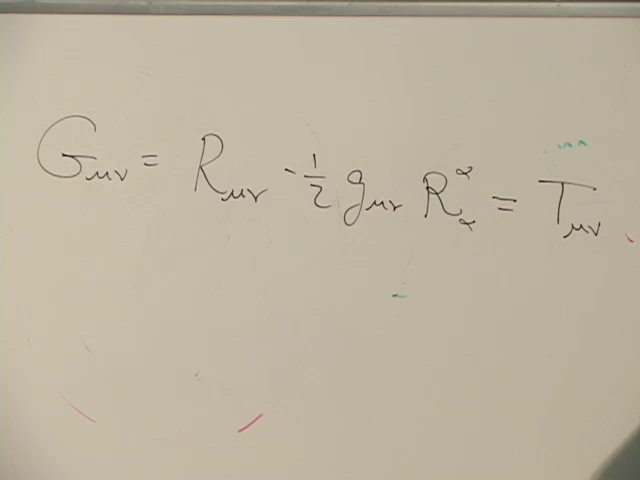
\includegraphics[width=0.74\textwidth]{lecture_09_figure_04.png}\caption{진공 수축으로 이중 진동자 합이 단일 합으로 줄어든다.}\lectureframe{00:20:10}\label{fig:l09-vacuum-contraction}\end{figure}

따라서
\begin{equation}
  \expect{\bigl(X(\sigma)-X_{\mathrm{cm}}\bigr)^2}_0
  \sim
  \sum_{n=1}^{\infty}\frac{\cos^2(n\sigma)}{n}.
  \label{eq:l09-size-single-sum}
\end{equation}
끈을 따라 일반적인 한 지점에서, 또는 \(\sigma\)에 대해 평균을 내면 \(\cos^2(n\sigma)\)는 대략 \(1/2\)가 된다. 모드 절단값을 \(N\)이라 하면,
\begin{equation}
  \expect{\bigl(X-X_{\mathrm{cm}}\bigr)^2}_{0,N}
  \sim
  \frac{1}{2}\sum_{n=1}^{N}\frac{1}{n}
  =\frac{1}{2}\log N+O(1).
  \label{eq:l09-logarithmic-size}
\end{equation}

\begin{figure}[H]\centering
  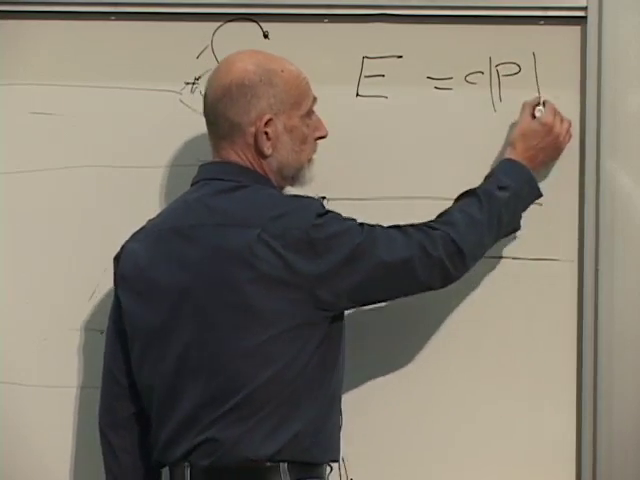
\includegraphics[width=0.72\textwidth]{lecture_09_figure_05.png}\caption{바닥 상태의 퍼짐을 좌우하는 조화급수에 이르는 칠판 유도.}\lectureframe{00:22:05}\label{fig:l09-harmonic-size}\end{figure}

예를 들어 처음 스물다섯 개 모드만 남기면 유한한 퍼짐을 가진 흐릿한 물체를 얻지만, 아직 연속적인 끈은 아니다. 절단값을 없애면 평균 제곱 퍼짐은 로그에 비례해 커진다. 이 결론을 평탄한 공간의 끈 이론이 비일관적이라는 증명으로 오해해서는 안 된다. 평탄한 공간에서는 질량중심 운동과 진동자 운동이 분리되며, 물리적 진폭에서의 섬세한 상쇄가 예상되는 국소성을 보존한다. 크기가 커진다는 것은 경고다. 곡률은 그 경고가 실제 실패로 이어지는지 알려 준다.

\section{내부 퍼짐이 기하를 바꿀 때}

끈을 구의 북극 근처에 놓자. 모든 진동자를 끈 상태에서는 방금 살펴본 점입자처럼 거동한다. 더 높은 모드를 허용하면 끈은 구면의 뚜껑 영역에 퍼진 요동하는 뒤엉킴이 된다. 질량중심은 여전히 구면을 따라 움직일 수 있지만, 회전 에너지에 들어가는 관성 모멘트의 대상은 이제 퍼져 있는 물체다.

구의 중심과 극을 지나는 축에 대해서는
\begin{equation}
  I=\int r_\perp^2\,dm,
  \label{eq:l09-extended-inertia}
\end{equation}
여기서 \(r_\perp\)는 끈의 한 요소와 축 사이의 수직 거리다. 궤도의 적도에 있는 점은 관련 지렛팔이 가장 길다. 축 쪽으로 처진 끈의 부분은 기여가 더 작다. 전체 질량을 고정하면 유효 관성 모멘트는 작아진다:
\begin{equation}
  I_{\mathrm{eff}}<mR^2.
  \label{eq:l09-inertia-reduction}
\end{equation}
따라서 회전 에너지는 더 작은 구면 위의 점물체 에너지처럼 보인다:
\begin{equation}
  E_{\mathrm{rot}}
  =\frac{L^2}{2I_{\mathrm{eff}}}
  \equiv \frac{L^2}{2mR_{\mathrm{eff}}^2},
  \qquad R_{\mathrm{eff}}<R.
  \label{eq:l09-effective-radius}
\end{equation}

\begin{classroomqa}\audiencequestion{끈이 더 넓은 영역으로 퍼지는데 관성 모멘트는 왜 0에 가까워져야 하나요? \lecturetimestamp{00:33:23}}\lecturerresponse{이는 퍼져 있는 원래 분포의 관성 모멘트가 즉시 0이 된다는 뜻이 아니라, 연속적인 거친 분해능 조정에 따른 유효 기술에 관한 말이다. 첫 번째 모드 띠는 점을 흐릿한 덩어리로 바꾸어 더 작은 구면 위에 있는 것처럼 움직이게 한다. 다음 띠는 각 덩어리 내부의 구조를 분해하고 같은 재규격화를 반복한다. 이 비교를 되풀이하면 유효 반지름은 안쪽으로 줄어든다.}\end{classroomqa}

\begin{figure}[H]
  \centering
  \includegraphics[width=0.72\textwidth]{lecture_09_figure_06.png}
  \medskip

  \begin{adjustbox}{max width=\linewidth}
  \begin{tikzpicture}[x=1cm,y=1cm,>=Latex]
    \draw[thick] (0,0) circle (2.15);
    \draw[dashed] (0,-2.55) -- (0,2.55);
    \draw[blue!65!black,thick]
      (-0.22,2.05)
      .. controls (-1.22,1.75) and (-1.52,1.08) .. (-1.06,0.44)
      .. controls (-0.55,-0.10) and (0.35,0.02) .. (1.10,0.68)
      .. controls (1.48,1.12) and (1.16,1.80) .. (0.20,2.05);
    \draw[red!70!black,dashed] (0,0) circle (1.25);
    \draw[->] (2.70,1.55) -- (4.05,1.55);
    \node[align=center] at (3.37,1.98) {add shorter\\modes};
    \draw[thick] (6.15,0) circle (1.25);
    \draw[dashed] (6.15,-1.65) -- (6.15,1.65);
    \draw[blue!65!black,thick]
      (6.00,1.18)
      .. controls (5.42,0.88) and (5.46,0.25) .. (6.02,-0.06)
      .. controls (6.46,-0.28) and (6.90,0.45) .. (6.28,1.18);
    \node at (0,-3.00) {sphere of radius \(R\)};
    \node at (6.15,-2.05) {effective radius \(R_{\mathrm{eff}}\)};
  \end{tikzpicture}
  \end{adjustbox}\caption{칠판에 그린 북극의 끈과 유효 반지름 논증을 깔끔하게 다시 그린 그림. 점선으로 표시한 안쪽 원은 유효 기하이지, 구 안에 들어 있는 두 번째 물리적 껍질이 아니다.}\lectureframe{00:35:15}\label{fig:l09-shrinking-sphere}\end{figure}

이는 재규격화군에 관한 진술이다. 유한한 절단값에서는 끈이 유한한 내부 분해능을 가진 덩어리로 보인다. 절단값을 높이면 그 덩어리의 역학이 바뀐다. 양의 곡률을 가진 구면에서는 모드 껍질을 하나씩 더 포함할 때마다 장거리 운동으로 추론하는 배경이 더 작아진다. 결과가 끝내 안정되지 않는다면 그 배경 위에는 절단값과 무관한 끈 이론이 존재하지 않는다.

\section{계량은 고정점에 도달해야 한다}

이제 구를 일반적인 표적 공간 계량 \(g_{\mu\nu}(x)\)으로 바꾸자. 진동자 모드의 얇은 로그 껍질에 대해 적분하면 계량은 국소적인 대칭 이계 텐서만큼 변한다. 이 변화는 평탄한 공간에서는 사라져야 하고, 계량의 두 미분을 포함하는 항에서 시작해야 한다. 선도 차수에서는 공변성에 따라 리치 텐서가 관련 후보로 남는다:
\begin{equation}
  \frac{\partial g_{\mu\nu}}{\partial\log\Lambda}
  =-C\,R_{\mu\nu}+\cdots ,
  \qquad C>0
  \label{eq:l09-ricci-flow}
\end{equation}
이는 기하학적 논증에서 사용한 조대화 방향을 따른 결과다. 따라서 양의 곡률은 구를 안쪽으로 수축시키며, 이는 요구된 바와 같다.
\editorialnote{정규화와 부호는 재규격화 매개변수가 자외선 쪽으로 증가하는지 적외선 쪽으로 증가하는지에 따라 달라진다. 통상적인 세계면 표기법에서 선도 차수의 계량 베타 함수는 \(\beta^g_{\mu\nu}=\alpha'R_{\mu\nu}+\cdots\)이다. 여기서 사용하는 불변적인 진술은 컷오프 독립성을 위해 베타 함수, 따라서 이 차수에서는 \(R_{\mu\nu}\)가 영이어야 한다는 것이다.}

\begin{figure}[H]\centering
  \includegraphics[width=0.76\textwidth]{lecture_09_figure_07.png}\caption{계량 변화는 리치 텐서의 음수에 비례하는 형태로 개략적으로 쓰고, 옆에는 매끄럽게 다듬어지는 곡선을 그렸다.}\lectureframe{00:43:00}\label{fig:l09-ricci-flow-board}\end{figure}

\begin{classroomqa}\audiencequestion{이 흐름 방정식에서 진동자 절단값 \(N\)은 어디에 나타나나요? \lecturetimestamp{00:43:38}}\lecturerresponse{그것이 척도 변수다. 포함하는 최고 모드가 바뀔 때 끈 크기 합은 로그에 따라 변하므로, 자연스러운 진화 매개변수는 \(\log N\), 또는 이와 동등하게 \(\log\Lambda\)이다. 식 \eqref{eq:l09-ricci-flow}은 모드의 로그 껍질 하나가 일으키는 미소 변화를 나타낸다.}\end{classroomqa}

허용 가능한 배경은 이 흐름의 고정점이다. 선도 차수에서는
\begin{equation}
  \boxed{R_{\mu\nu}=0.}
  \label{eq:l09-ricci-flat}
\end{equation}
리치 평탄하다고 해서 리만 텐서의 모든 성분이 영인 것은 아니다. 예를 들어 중력파는 \(R_{\mu\nu}=0\)를 만족하면서도 진공에서 영이 아닌 곡률을 가질 수 있다.

\subsection{같은 조건은 진공 아인슈타인 방정식이다}

통상적인 상수들을 생략하면 아인슈타인 방정식은 다음과 같다.
\begin{equation}
  G_{\mu\nu}
  \equiv
  R_{\mu\nu}-\frac12 g_{\mu\nu}R
  =T_{\mu\nu}.
  \label{eq:l09-einstein}
\end{equation}

\begin{figure}[H]\centering
  \includegraphics[width=0.78\textwidth]{lecture_09_figure_08.png}\caption{칠판에 적힌 아인슈타인 텐서와 응력 텐서.}\lectureframe{00:47:15}\label{fig:l09-einstein-board}\end{figure}

진공에서는 \(T_{\mu\nu}=0\)이다. \(D\) 시공간 차원에서 \begin{equation}
  0=g^{\mu\nu}G_{\mu\nu}
   =\left(1-\frac{D}{2}\right)R.
  \label{eq:l09-einstein-trace}
\end{equation}
\(D\neq2\)이면 \(R=0\)이고, 이를 \eqref{eq:l09-einstein}에 대입하면 \(R_{\mu\nu}=0\)를 얻는다. 따라서 끈의 컷오프 의존성이 사라지려면 진공 중력장 방정식이 성립해야 한다. 중력은 이론에 덧붙여진 것이 아니라, 일관성을 유지하기 위해 치러야 하는 대가로 나타났다.

\emph{진공}이라는 말은 아무 일도 일어나지 않는다는 뜻이 아니다. 해당 영역에 응력-에너지 원천이 없다는 뜻이다. 원천이 없는 맥스웰 방정식은 전자기파를 허용하고, 원천이 없는 아인슈타인 방정식은 중력파를 허용한다. 리치 텐서가 영이어도 기하학은 시간에 따라 변할 수 있다.

\begin{classroomqa}\audiencequestion{이 조건은 등각 불변성과 관련이 있나요?
\lecturetimestamp{00:52:20}}\lecturerresponse{그렇다. 다만 녹음에서는 질문의 일부가 잘려 있다. 관련 대칭은 양자 \emph{세계면}의 등각 불변성이다. 세계면 척도 변칙이 사라지도록 요구하면 계량 베타 함수가 0이 된다. 이를 시공간 자체의 등각 불변성을 요구하는 것과 혼동해서는 안 된다.}\end{classroomqa}

두 번째 일관성 조건도 있다. 세계면 등각 불변성은 임계 시공간 차원도 정한다. 초끈 이론에서는 10차원, 보손 끈 이론에서는 26차원이다. 따라서 리치 평탄성만으로 요구 조건 전체가 충족되지는 않지만, 아인슈타인 방정식을 가장 직접적으로 드러내는 부분은 바로 이것이다.

\section{사라진 차원이 아니라 콤팩트한 차원}

초끈 배경에는 공간 차원 9개와 시간 차원 1개가 있다. 거시적인 우리 세계에서 드러나는 큰 공간 방향은 3개뿐이므로, 나머지 공간 차원 6개는 숨겨져 있거나 보통의 척도에서 접근할 수 없게 되어 있어야 한다. 콤팩트화는 이 차원들을 실제 방향으로 남겨 두면서도 유한하고 작은 크기를 갖게 한다.

\begin{classroomqa}\audiencequestion{관찰자마다 다른 시계를 가지고 있다면 시간 차원이 둘 이상이라는 뜻인가요? \lecturetimestamp{00:56:59}}\lecturerresponse{아니다. 여러 시계는 하나의 시공간에서 좌표를 측정하는 여러 계측기일 뿐이며, 서로 독립적인 시간꼴 방향을 만들어 내지 않는다. 여기서 다루는 추가 차원은 공간 차원이다. 익숙한 양자 및 인과 구조로는 국소적인 시간 방향이 여러 개인 일관된 이론을 비슷하게 구성할 수 없으므로, 그런 가능성은 이 콤팩트화 모형에 포함되지 않는다.}\end{classroomqa}

자신들의 세계가 선이라고 믿는 생명체를 상상해 보자. 낮은 분해능에서는 앞뒤로만 움직일 수 있다. 하지만 충분히 강력한 현미경으로 보면 그 선은 매우 가느다란 원기둥으로 드러난다. 작은 생명체는 길이 방향뿐 아니라 원형 방향으로도 움직일 수 있다. 두 번째 방향은 처음부터 있었지만, 둘레가 너무 작아 거친 탐사로는 분해할 수 없었던 것이다.

\begin{figure}[H]\centering
  \includegraphics[width=0.78\textwidth]{lecture_09_figure_09.png}\caption{숨겨진 원형 방향을 따라 감기는 궤적이 있는 가느다란 원기둥.}\lectureframe{01:01:00}\label{fig:l09-hidden-cylinder}\end{figure}

원기둥은 위쪽과 아래쪽 가장자리를 서로 동일시한 띠로 나타낼 수 있다. 위쪽 가장자리로 나가면 같은 길이 좌표의 아래쪽 가장자리로 돌아온다. 어느 가장자리에도 물리적인 경계는 없다. 두 방향에도 같은 조작을 할 수 있다. 직사각형의 왼쪽과 오른쪽 가장자리를 동일시하고, 위쪽과 아래쪽 가장자리도 동일시하는 것이다. 그 결과가 2차원 토러스다.

\begin{figure}[H]
  \centering
  \includegraphics[width=0.76\textwidth]{lecture_09_figure_10.png}
  \medskip

  \begin{tikzpicture}[x=0.82cm,y=0.82cm,>=Latex]
    \draw[thick] (0,0) rectangle (4,2.15);
    \draw[blue!65!black,->] (0,2.48) -- (4,2.48);
    \draw[blue!65!black,->] (4,-0.34) -- (0,-0.34);
    \node at (2,-0.82) {one periodic direction};
    \draw[thick] (6.1,0) rectangle (10.1,2.15);
    \draw[blue!65!black,->] (6.1,2.48) -- (10.1,2.48);
    \draw[blue!65!black,->] (10.1,-0.34) -- (6.1,-0.34);
    \draw[red!70!black,->] (5.76,0) -- (5.76,2.15);
    \draw[red!70!black,->] (10.44,2.15) -- (10.44,0);
    \node at (8.1,-0.82) {two periodic directions};
  \end{tikzpicture}\caption{칠판의 판 모양 그림과 기본 영역을 깔끔하게 다시 그린 그림. 한 쌍의 가장자리를 동일시하면 원기둥이 되고, 두 쌍을 모두 동일시하면 토러스가 된다.}\lectureframe{01:04:40}\label{fig:l09-periodic-identification}\end{figure}

토러스는 먼저 위상 공간이며, 3차원 공간 안의 도넛 모양 곡면인 것은 그다음이다. 토러스를 한 번 자르면 원기둥이 되고, 가장자리 동일시를 기억해 두면 한 번 더 잘라 직사각형이 된다. 이 직사각형에 평탄한 계량을 줄 수 있으므로, 이렇게 얻은 평탄 토러스는 국소적으로 리만 곡률이 0이며 당연히 리치 평탄하다.

직사각형 위의 직선 궤적은 동일시된 가장자리를 지나서도 곧게 이어진다. 기울기가 두 주기의 유리수 비라면 궤적은 결국 닫힌다. 그 비가 무리수라면 궤적은 닫히지 않고 토러스 위를 조밀하게 채운다.

\begin{figure}[H]\centering
  \includegraphics[width=0.76\textwidth]{lecture_09_figure_11.png}\caption{기본 영역 안의 반복되는 직선 선분은 토러스 위에서 중단 없이 이어지는 하나의 궤적을 나타낸다.}\lectureframe{01:11:00}\label{fig:l09-torus-trajectory}\end{figure}

고차원 토러스도 같은 방식으로 만든다. 서로 마주 보는 각 면 쌍을 동일시한 정육면체는 3차원 토러스이고, 6개의 콤팩트 차원은 6차원 토러스로 모형화할 수 있다. 이 물체들을 보통의 3차원 공간 안에 모두 끼워 넣으려 해서는 안 된다. 면을 동일시하는 설명만으로 내재적으로 완전하게 기술할 수 있다.

\begin{classroomqa}\audiencequestion{추가 차원은 반드시 다시 자기 자신과 이어져야 하나요?
\lecturetimestamp{01:15:03}}\lecturerresponse{정리상 반드시 그런 것은 아니다. 비콤팩트 차원일 수도 있지만, 그러면 보통 관측되는 장거리 세계에 또 하나의 큰 방향으로 나타날 것이다. 추가 차원이 없는 것처럼 보이는 현상과 양립하는 가장 간단한 방법은 콤팩트하게 만드는 것이다. 자연이 특정한 콤팩트화를 선택하는 이유는 별개의 동역학적 질문이다.}\end{classroomqa}

\begin{classroomqa}\audiencequestion{보이지 않는 차원이 이런 식으로 말린 보통의 공간 방향이라고 가정하는 이유는 무엇인가요? 완전히 다른 것일 수도 있지 않나요? \lecturetimestamp{01:15:51}}\lecturerresponse{이 가설이 자연을 기술하는 유일한 방식이라고 증명되었기 때문이 아니라, 명확하고 풀 수 있는 가설이기 때문이다. 콤팩트 공간 다양체를 이용하면 일관된 사례를 구성하고 그 스펙트럼을 계산할 수 있다. 더 이국적인 가능성도 같은 일을 해내야 받아들일 근거를 얻는다.}\end{classroomqa}

\begin{classroomqa}\audiencequestion{익숙한 도넛 모양 토러스에서의 거리는 직사각형에서의 거리처럼 보이지 않습니다. 어떤 기하를 뜻하나요?
\lecturetimestamp{01:18:11}}\lecturerresponse{\emph{토러스}라는 말은 동일시 방법을 정할 뿐, 유일한 계량을 정하지는 않는다. 공간에 끼워 넣은 도넛은 3차원 공간에서 유도된 곡률 있는 계량을 갖는다. 주기적으로 가장자리를 동일시한 직사각형은 평탄한 계량을 갖는다. 두 공간은 위상은 같지만 기하는 다르다. 간단한 콤팩트화에서 말하는 것은 평탄한 쪽이다.}\end{classroomqa}

\section{평탄 토러스의 모양 매개변수}

평탄한 2차원 토러스도 하나로 정해지지 않는다. 기본 평행사변형에는 전체 면적, 종횡비, 그리고 전단이 있다. 이 매개변수들을 바꾸면 위상은 그대로지만 거리가 달라지고, 따라서 스펙트럼도 달라진다.

\begin{figure}[H]
  \centering
  \includegraphics[width=0.74\textwidth]{lecture_09_figure_12.png}
  \medskip

  \begin{tikzpicture}[x=0.9cm,y=0.9cm,>=Latex]
    \draw[thick] (0,0) rectangle (3.4,2.1);
    \draw[<->] (0,-0.35) -- node[below] {\(L_1\)} (3.4,-0.35);
    \draw[<->] (-0.35,0) -- node[left] {\(L_2\)} (-0.35,2.1);
    \draw[thick] (5.4,0) -- (8.8,0) -- (9.7,2.1) -- (6.3,2.1) -- cycle;
    \draw[dashed] (5.4,0) -- (6.3,2.1);
    \draw[->] (5.75,2.48) -- node[above] {shear} (6.45,2.48);
    \node at (1.7,-1.00) {area and aspect ratio};
    \node at (7.55,-1.00) {complex structure};
  \end{tikzpicture}\caption{토러스 모듈라이를 설명하는 데 사용하는 직사각형 및 전단된 기본 영역.}\lectureframe{01:23:00}\label{fig:l09-torus-moduli}\end{figure}

2차원 토러스에서는 모양을 복소수 \(\tau=\tau_1+i\tau_2\) 하나로 나타내면 편리하다. 실수부는 전단을 기록하고, 전체 척도를 분리한 뒤 허수부는 종횡비를 기록한다. 두 기본 주기를 서로 바꾸거나 정수 기저를 바꾸면, 겉보기에 다른 평행사변형이 같은 토러스를 나타낼 수 있다.

\begin{classroomqa}\audiencequestion{동일시하기 전에 한쪽 가장자리를 뒤집으면 어떻게 되나요? \lecturetimestamp{01:24:20}}\lecturerresponse{위상이 달라진다. 반사해서 동일시하면 보통의 토러스가 아니라 비가향 곡면인 클라인 병이 된다.}\end{classroomqa}

\begin{classroomqa}\audiencequestion{가장자리를 따라 비틀림이 일정하지 않으면 어떻게 되나요?
\lecturetimestamp{01:25:01}}\lecturerresponse{매끄럽고 일정하지 않은 변형은 기본 영역의 계량으로 옮겨 담을 수 있다. 위상적 동일시와 기하학적 자료는 구분해서 다뤄야 한다. 붙이는 방식을 바꾸면 위상이 달라질 수 있지만, 거리를 매끄럽게 바꾸면 계량이 달라진다.}\end{classroomqa}

\editorialnote{평탄한 2차원 토러스에서 면적은 가장 단순한 칼러 모듈러스이며, \(\tau\)는 복소구조 모듈러스다. 연속적인 전단은 \(\tau\)의 일부다. 반면 데ーン 비틀기는 이산적인 사상류 연산으로, \(\tau\mapsto\tau+1\)로 나타낸다. 이것 자체가 연속 모듈러스인 것은 아니다. 이는 칠판 논의에서 의도적으로 비격식적으로 사용한 용어를 더 정확히 다듬은 것이다.}

평탄 토러스는 일관성 조건을 즉시 만족하므로 유용하지만, 대칭성이 지나치게 커서 현실적인 입자물리학 모형에는 적합하지 않다. 칼라비--야우 다양체처럼 더 복잡한 리치 평탄 공간은 더 풍부한 콤팩트화를 제공한다. 그 구체적인 구성은 이 논의의 범위를 벗어나지만, 기본 원리는 같다.

\section{스펙트럼에서 콤팩트 원 읽어내기}

휴식 후에는 콤팩트 공간을 둘레가 \(2\pi R\)인 원 하나로 줄여 보자. 파동함수는 원을 한 바퀴 돈 뒤 단일값이어야 한다:
\begin{equation}
  e^{ip_c(x+2\pi R)/\hbar}=e^{ip_cx/\hbar}.
\end{equation}
따라서
\begin{equation}
  p_cR=n\hbar,
  \qquad
  p_c=\frac{n\hbar}{R},
  \qquad n\in\mathbb Z.
  \label{eq:l09-kk-momentum}
\end{equation}

\begin{figure}[H]\centering
  \includegraphics[width=0.74\textwidth]{lecture_09_figure_13.png}\caption{\(2\pi R\)와 양자화된 운동량 \(p_c=n\hbar/R\).}\lectureframe{01:32:15}\label{fig:l09-kk-board}\end{figure}

전체 시공간에서 질량이 없는 입자의 경우,
\begin{equation}
  E=c|\mathbf P|.
  \label{eq:l09-massless-dispersion}
\end{equation}

\begin{figure}[H]\centering
  \includegraphics[width=0.70\textwidth]{lecture_09_figure_14.png}\caption{콤팩트 운동량을 저차원 질량으로 재해석하는 데 쓰이는 질량 없는 입자의 분산 관계.}\lectureframe{01:33:45}\label{fig:l09-massless-board}\end{figure}

운동량을 비콤팩트 성분과 콤팩트 성분으로 나누고 \(c=\hbar=1\)로 놓자:
\begin{equation}
  E^2=\mathbf p_{\mathrm{large}}^2+\frac{n^2}{R^2}.
  \label{eq:l09-kk-dispersion}
\end{equation}
콤팩트 방향을 분해할 수 없는 관찰자는 이를 \(E^2=\mathbf p_{\mathrm{large}}^2+m^2\)와 비교하여 질량 탑을 추론한다:
\begin{equation}
  m_n=\frac{|n|}{R}.
  \label{eq:l09-kk-masses}
\end{equation}
\(n\)의 두 부호는 양의 에너지를 갖는 반대 방향의 콤팩트 운동량을 나타내며, 양의 질량과 음의 질량을 뜻하지 않는다. 따라서 간격 \(1/R\)을 분광학적으로 측정하면 반지름을 알아낼 수 있다. 이것이 칼루차--클라인 기작이다. 숨겨진 방향의 운동량이 보이는 차원에서는 질량으로 나타난다.

\section{감김 상태가 스펙트럼을 완성한다}

닫힌 끈에는 점입자에게 없는 가능성이 있다. 원을 감을 수 있다는 것이다. 감김수가 \(w\)라면 끈은 콤팩트 방향을 \(w\)번 돈 뒤에야 닫힌다. 끈의 길이는 \(2\pi |w|R\)이므로 장력에 따라 에너지가 생긴다:
\begin{equation}
  m_w
  =2\pi T\,|w|R
  =\frac{|w|R}{\alpha'}.
  \label{eq:l09-winding-mass}
\end{equation}
강의에서는 \(\alpha'=1\)인 단위를 선택하여 다음처럼 쓴다:
\begin{equation}
  m_w=|w|R.
  \label{eq:l09-winding-lecture-units}
\end{equation}
\(w\)의 양수와 음수는 원을 도는 방향이 서로 반대임을 나타낸다.

\begin{figure}[H]\centering
  \includegraphics[width=0.76\textwidth]{lecture_09_figure_15.png}\caption{칠판에 표시한 콤팩트 반지름과 함께 콤팩트 원기둥을 감은 닫힌 끈.}\lectureframe{01:39:45}\label{fig:l09-winding-board}\end{figure}

따라서 콤팩트 원은 서로 보완적인 두 탑을 만든다:
\begin{equation}
  m_n=\frac{|n|}{R},
  \qquad
  m_w=\frac{|w|R}{\alpha'}.
  \label{eq:l09-two-towers}
\end{equation}
\(R\)가 클 때 운동량 준위의 간격은 촘촘하고 감김 상태는 무겁다. \(R\)가 작을 때는 운동량 준위의 간격이 넓고 감김 상태는 가볍다.

\begin{figure}[H]\centering
  \begin{tikzpicture}[x=1cm,y=0.9cm,>=Latex]
    \draw[->] (0,0) -- (0,4.7) node[above] {\(m\)};
    \foreach \y/\lab in {0/0,1.1/{1/R},2.2/{2/R},3.3/{3/R},4.4/{4/R}} {
      \draw (-0.16,\y) -- (0.16,\y);
      \node[left] at (-0.22,\y) {\(\lab\)};
    }
    \node at (0,-0.62) {momentum};
    \draw[<->,very thick,blue!65!black] (2.05,2.15) -- (4.05,2.15)
      node[midway,above] {\(R\leftrightarrow\alpha'/R\)};
    \draw[->] (6.1,0) -- (6.1,4.7) node[above] {\(m\)};
    \foreach \y/\lab in {0/0,1.1/{R/\alpha'},2.2/{2R/\alpha'},3.3/{3R/\alpha'},4.4/{4R/\alpha'}} {
      \draw (5.94,\y) -- (6.26,\y);
      \node[right] at (6.32,\y) {\(\lab\)};
    }
    \node at (6.1,-0.62) {winding};
  \end{tikzpicture}\caption{반지름을 끈 단위로 역수화하면 운동량 탑과 감김 탑이 서로 바뀐다.}\label{fig:l09-dual-mass-towers}\end{figure}

\section{T-쌍대성: 작은 원과 큰 원은 같은 물리학이다}

두 탑은 다음 변환으로 서로 바뀐다:
\begin{equation}
  R\longleftrightarrow\frac{\alpha'}{R},
  \qquad
  n\longleftrightarrow w.
  \label{eq:l09-t-duality}
\end{equation}
칠판에서 사용한 단위에서는 \(\alpha'=1\)이므로, 이는 간단히 \(R\leftrightarrow1/R\)가 된다. 자기쌍대 반지름 \(R=\sqrt{\alpha'}\)에서는 운동량과 감김의 척도가 일치한다.

\begin{figure}[H]\centering
  \includegraphics[width=0.74\textwidth]{lecture_09_figure_16.png}\caption{반지름이 자기쌍대 척도를 지날 때 칠판에서 비교한 성긴 질량 준위와 촘촘한 질량 준위.}\lectureframe{01:43:00}\label{fig:l09-duality-board}\end{figure}

기본 질량 공식들이 서로 바뀐다는 것은 결과의 겉으로 드러난 일부에 불과하다. 닫힌 끈의 진동자 상태와 산란 진폭도 일관되게 대응된다. 끈 척도보다 작은 원은 계속 더 작아지는 새로운 기하가 아니라, 더 큰 쌍대 원으로 동등하게 기술된다. 점입자에는 운동량 모드만 있고 감김 모드는 없으므로 이런 대응을 만들 수 없다.

\begin{classroomqa}\audiencequestion{수직 방향과 수평 방향을 서로 바꾸는 것과 같은 뜻인가요? \lecturetimestamp{01:44:38}}\lecturerresponse{아니다. 서로 다른 두 양자수, 즉 원을 따라 도는 운동량과 닫힌 끈이 원을 감는 횟수를 서로 바꾸는 것이다. 이와 동시에 반지름을 역수화해야 한다.}\end{classroomqa}

\begin{classroomqa}\audiencequestion{\(R<\sqrt{\alpha'}\)와 \(R>\sqrt{\alpha'}\)에서 비교하는 기술은 보손에만 해당하나요, 페르미온에도 해당하나요?
\lecturetimestamp{01:46:30}}\lecturerresponse{이 쌍대성은 이를 설명하기 위해 사용한 단순한 보손 질량 탑만의 대칭이 아니라, 콤팩트화된 끈 이론 전체의 대칭이다. 각 부문의 구체적인 대응은 이론에 따라 다르지만, 작은 원과--큰 원의 동등성은 특정 입자 종류에 한정되지 않는다.}\end{classroomqa}

\begin{classroomqa}\audiencequestion{비교하는 두 상태는 열린 끈인가요, 닫힌 끈인가요? \lecturetimestamp{01:47:32}}\lecturerresponse{닫힌 끈 상태다. 자유롭게 전파되는 닫힌 끈은 콤팩트 원을 감을 수 있다. 끝점이 자유로운 보통의 열린 끈은 같은 보존 감김수를 갖지 않는다.}\end{classroomqa}\editorialnote{더 완전한 열린 끈 설명에서는 T-쌍대성이 노이만 경계 조건과 디리클레 경계 조건을 서로 바꾸고 D-막을 도입한다. 그래서 열린 끈의 T-쌍대성은 닫힌 끈의 감김 공식을 단순히 그대로 옮기는 것보다 풍부하다.}

\begin{classroomqa}\audiencequestion{이 대응은 블랙홀 지평선 근처에서 공간과 시간이 서로 바뀌는 것과 비슷한가요? \lecturetimestamp{01:48:00}}\lecturerresponse{아니다. 지평선 좌표와 인과적 성격은 다른 문제다. 여기서 두 기술은 하나의 콤팩트한 공간 원과 그 운동량 부문 및 감김 부문의 교환을 다룬다.}\end{classroomqa}

\begin{classroomqa}\audiencequestion{이로써 최소 길이를 도입해 짧은 거리 자기 에너지 문제를 해결하나요? \lecturetimestamp{01:48:35}}\lecturerresponse{끈 척도보다 작은 반지름은 서로 동등하지 않은 새로운 원 배경을 정의하지 않는다는 것을 보여 준다. 자기쌍대점을 지나 \(R\)를 줄이면 쌍대 반지름은 커진다. 이는 임의로 작은 원 기하를 탐사하지 못하게 하는 정밀한 끈 이론적 제약이다. 다만 이를 모든 가능한 거리 개념에 보편적인 엄격한 하한이 있다는 주장으로 확대해서는 안 된다.}\end{classroomqa}

\section{감김 부문을 생략할 수 없는 이유}

\begin{classroomqa}
\audiencequestion{감기지 않은 끈만으로 이론을 정의하고 감김 상태는 제외할 수 있을까요? \lecturetimestamp{01:48:56}}
\lecturerresponse{아니요. 닫힌 끈의 상호작용으로 감김 상태가 생성됩니다. 감기지 않은 고리를 늘여 콤팩트한 방향을 감싸게 하면, 한 구간은 원을 한쪽 방향으로 돌고 다른 구간은 반대 방향으로 돕니다. 순감김수는 여전히 0입니다. 그러면 재접속으로 고리가 감김수가 \(+1\)인 닫힌 끈 하나와 \(-1\)인 닫힌 끈 하나로 나뉠 수 있습니다. 이 두 끈은 서로 멀어질 수 있으므로, 초기 상태에 감김이 전혀 없더라도 감김 상태는 스펙트럼에 포함되어야 합니다.}
\end{classroomqa}

\begin{figure}[H]
\centering
  \includegraphics[width=0.74\textwidth]{lecture_09_figure_17.png}
  \caption{재접속 전, 콤팩트한 방향을 감싸도록 배치한 늘어난 영감김 고리.}
  \lectureframe{01:50:30}
  \label{fig:l09-winding-pair-before}
\end{figure}

\begin{figure}[H]
  \centering
  \includegraphics[width=0.72\textwidth]{lecture_09_figure_18.png}
  \medskip

  \begin{tikzpicture}[x=0.9cm,y=0.9cm,>=Latex]
    \draw[thick] (0,0) ellipse (1.0 and 1.55);
    \draw[blue!65!black,thick]
      (0.08,1.35) .. controls (2.0,1.15) and (2.0,-1.15) .. (0.08,-1.35);
    \draw[red!70!black,thick]
      (-0.08,-1.35) .. controls (-2.0,-1.15) and (-2.0,1.15) .. (-0.08,1.35);
    \node at (0,-2.15) {net \(w=0\)};
    \draw[->,thick] (2.45,0) -- (3.75,0) node[midway,above] {split};
    \draw[thick] (5.05,0.62) ellipse (0.68 and 1.02);
    \draw[blue!65!black,very thick,->]
      (5.05,1.64) arc[start angle=90,end angle=-250,x radius=0.68,y radius=1.02];
    \node at (5.05,-0.82) {\(w=+1\)};
    \draw[thick] (7.45,0.62) ellipse (0.68 and 1.02);
    \draw[red!70!black,very thick,<-]
      (7.45,1.64) arc[start angle=90,end angle=-250,x radius=0.68,y radius=1.02];
    \node at (7.45,-0.82) {\(w=-1\)};
  \end{tikzpicture}
  \caption{칠판에 그린 서로 분리된 감긴 고리와 감김--반감김 쌍 생성의 깔끔한 재구성. 전체 감김수는 여전히 0이다.}
  \lectureframe{01:51:30}
  \label{fig:l09-winding-pair-after}
\end{figure}

\begin{classroomqa}
\audiencequestion{감김 쌍을 생성하려면 추가 에너지가 필요한가요?
\lecturetimestamp{01:52:11}}
\lecturerresponse{네. 끈을 늘이는 데 장력 에너지가 들고, 최종 상태의 감긴 끈들은 \eqref{eq:l09-winding-mass}에 주어진 질량을 가집니다. 충분히 에너지가 큰 충돌이라면 이 쌍을 생성할 수 있습니다. 이는 관련 보존 전하를 보존하면서 충돌로 입자와 반입자를 생성할 수 있는 것과 같습니다.}
\end{classroomqa}

\section{끈 배경의 형태를 소리로 알아낼 수 있을까?}

일반적인 콤팩트화 입자 이론에서는 칼루차--클라인 스펙트럼의 간격으로부터 반지름을 추론할 수 있습니다. 즉, 정상 모드를 통해 콤팩트 공간의 형태를 알아내려 합니다. 끈 이론에서는 역문제가 더 미묘해집니다. 운동량 모드는 \(1/R\)를, 감김 모드는 \(R/\alpha'\)를 반영하며, 두 모드를 서로 바꾸어도 전체 스펙트럼은 변하지 않습니다. 점입자 기하학에서 서로 다른 것으로 여기는 두 반지름은 이중 변수로 표현한 하나의 끈 배경입니다.

따라서 이 강의는 하나의 경로를 따라 예고했던 두 결론에 모두 도달했습니다. 자외선 영역의 일관성을 위해 표적 계량은 진공 아인슈타인 방정식을 만족해야 하므로 중력은 불가피합니다. 이어지는 콤팩트화는 숨은 기하를 입자 스펙트럼으로 바꾸지만, 감김 상태 때문에 그 스펙트럼만으로는 끈 척도 아래의 고전적 반지름을 유일하게 정할 수 없습니다. 일관성은 허용되는 기하가 무엇인지 정할 뿐 아니라, T 이중성을 통해 무엇을 서로 다른 기하로 볼 것인지도 바꿉니다.

\chapter{T-이중성, D-브레인과 게이지 이론}

\lectureoverview{T-이중성은 반지름이 (R)인 원 위의 닫힌 끈과 \(\alpha'/R\)인 원 위의 닫힌 끈 사이의 정확한 동등성으로 시작한다. 운동량과 감김수의 역할이 서로 바뀌고, 세계면 미분 \(\partial_\tau Y\)와 \(\partial_\sigma Y\), 그리고 \(G_{\mu 5}\)와 \(B_{\mu 5}\)에서 유래하는 시공간 벡터장도 서로 바뀐다. 같은 변환을 열린 끈에 적용하면 노이만 끝점 조건이 디리클레 조건으로 바뀐다. 그러면 끝점은 동역학적 D-브레인 위에 놓여야 한다. 하나의 브레인에 붙들린 열린 끈은 저에너지에서 아벨 게이지 이론을 이루고, 브레인 더미를 잇는 끈은 양 끝점의 꼬리표를 지녀 비아벨 게이지 이론을 이룬다. D3-브레인에 끝나는 D-끈은 그에 대응하는 자기 홀극을 제공한다.}

\section{왜 T-이중성으로 돌아가는가?}

우리는 이미 T-이중성을 살펴보았지만, 여기에는 다시 다룰 이유가 있다. T-이중성은 끈 이론에 섭동적 끈보다 훨씬 많은 것이 들어 있음을 보여 준 단서 가운데 하나였다. 열린 끈에 미치는 결과를 이해하면서 D-브레인이 등장했고, 이어서 D-브레인은 양자장 이론을 구성하고 연구하는 방법이 되었다. 따라서 이 강의의 목적은 작은 원이 큰 원과 동등하다는 표어를 되풀이하는 데 그치지 않는다. 그 표어가 이론에 새로운 물리적 대상을 어떻게 불러들이는지 알 수 있도록 논증을 차근차근 다시 세워 보겠다.

가장 단순한 설정은 토러스 콤팩트화다. 1차원 토러스는 원이다. 2차원 토러스는 마주 보는 변을 서로 식별한 평행사변형으로 나타낼 수 있고, 3차원 토러스는 마주 보는 면을 서로 식별한 평행육면체로 나타낼 수 있다. 같은 구성은 더 높은 차원에서도 이어진다. 콤팩트한 공간 좌표 하나만 남겨 \(Y\)라 하고, 비콤팩트 좌표 하나를 대표로 두어 \(X\)라 하겠다. 시간도 있지만 칠판 그림에는 표시하지 않는다.

다음 표준 관례를 택하자.
\begin{equation}
  Y\sim Y+2\pi R,
  \label{eq:l10-circle-identification}
\end{equation}
이에 따라 \(R\)는 반지름이고 \(2\pi R\)는 원주다. 강의에서는 콤팩트 방향의 크기를 흔히 간단히 \(r\)라 하고 \(2\pi\)와 \(\alpha'\)의 인자를 생략한다. 유도 과정에서는 표준 인자를 유지하고, 유용한 경우에는 강의에서 사용한 단위계의 표현도 보이겠다.

논의의 전반부에서는 닫힌 유향 끈을 다룬다. 방향은 끈을 따라 그린 본질적인 화살표다. 어디서나 모든 화살표를 뒤집어도 실험 결과는 달라지지 않는다. 중요한 것은 두 끈 사이의 상대적 방향이다. 끈이 갈라지거나 합쳐질 때 화살표는 연속적으로 이어져야 한다. 이것은 부호를 지닌 보존량이 나타나리라는 첫 번째 단서다.

\begin{figure}[H]
  \centering
  \includegraphics[width=0.72\textwidth]{lecture_10_figure_01.png}
  \caption{칠판에 상대적 방향을 표시한 두 닫힌 끈. 분할과 결합 과정에서도 방향은 연속적이어야 한다.}
  \lectureframe{00:05:40}
  \label{fig:l10-oriented-closed-strings}
\end{figure}

\begin{classroomqa}
\audiencequestion{세계면 좌표가 \(\sigma=0\)에서 \(2\pi\)까지 변한다면, 끈은 이미 콤팩트 방향을 한 바퀴 돈 것인가? \lecturetimestamp{00:08:42}}
\lecturerresponse{아니다. 좌표 \(\sigma\)는 끈을 따라 있는 점들을 표시할 뿐, 콤팩트 공간에서의 위치를 표시하지 않는다. 감겼든 풀렸든 모든 닫힌 끈에는 주기 매개변수 \(\sigma\)가 있다. 고무줄의 비유가 도움이 된다. 고무줄을 아무것에도 감지 않았더라도 둘레를 따라 있는 분자에 번호를 매길 수 있다. 감김은 매개변수 \(\sigma\) 자체가 아니라 사상 \(Y(\tau,\sigma)\)의 성질이다.}
\end{classroomqa}

\begin{classroomqa}
\audiencequestion{콤팩트 방향의 크기도 큰 좌표 \(X\)의 모든 값에서 같아야 하나요? \lecturetimestamp{00:10:00}}
\lecturerresponse{일반적인 동역학적 콤팩트화에서는 그렇지 않다. 가장 단순한 배경인 고정된 원에서 시작하겠다. 나중에는 성분 \(G_{55}\)가 다섯 번째 방향의 국소적 크기를 나타내는 스칼라장이 되어, 그 크기가 보통 시공간에 걸쳐 달라질 수 있다.}
\end{classroomqa}

\section{끈들이 다시 연결되어도 감김수는 보존된다}

감기지 않은 끈은 감기지 않은 채 콤팩트 방향을 따라 움직일 수 있다. 감긴 끈은 다르다. \(\sigma\)가 닫힌 끈을 따라 한 바퀴 돌 때 매장 \(Y(\tau,\sigma)\)은 콤팩트 원의 주기를 하나 이상 진행한다. 끈에는 방향이 있으므로 진행 방향에는 부호가 붙는다. 끈은 양의 방향으로 감길 수도 있고 음의 방향으로 감길 수도 있다.

결합 그림을 보면 보존 법칙이 가장 분명하게 드러난다. 감김수 \(+1\)인 끈 하나와 감김수 \(-1\)인 다른 끈 하나를 생각하자. 두 끈의 방향이 맞는 구간은 다시 연결될 수 있다. 그렇게 얻은 배치의 총 감김수는 0이며, 이를 감기지 않은 끈으로 변형할 수 있다. 칠판 그림은 방향이 반대인 끈들이 다시 연결되는 바로 그 과정을 보여 준다.

\begin{figure}[H]
  \centering
  \includegraphics[width=0.72\textwidth]{lecture_10_figure_02.png}
  \medskip

  \begin{tikzpicture}[x=1cm,y=1cm,>=Latex]
    \draw[thick] (-4.0,0.3) circle (0.65);
    \draw[->,thick] (-4.55,0.58) arc (150:-145:0.65);
    \node at (-4.0,-0.65) {$w=+1$};
    \draw[thick] (-2.0,0.3) circle (0.65);
    \draw[<-,thick] (-2.55,0.58) arc (150:-145:0.65);
    \node at (-2.0,-0.65) {$w=-1$};
    \node at (-3.0,0.3) {$+$};
    \draw[->,thick] (-1.0,0.3) -- (0.3,0.3);
    \draw[thick] (1.4,0.3) ellipse (0.95 and 0.55);
    \node at (1.4,-0.65) {$w_{\rm total}=0$};
  \end{tikzpicture}
  \caption{반대 방향의 감김이 다시 연결되어 총 감김수가 0인 배치가 된다. 아래 그림은 칠판의 과정을 깔끔하게 다시 그린 것이며, 별도의 동역학적 과정이 아니다.}
  \lectureframe{00:13:20}
  \label{fig:l10-opposite-winding}
\end{figure}

이번에는 방향이 같은 끈 두 개로 실험을 반복해 보자. 이 끈들은 합쳐질 수 있지만 감김을 풀 수는 없다. 결과로 생긴 끈의 감김수는 들어온 각 끈의 감김수의 두 배다. 연결된 끈의 개수는 바뀌었지만 총 감김수는 바뀌지 않았다.

\begin{figure}[H]
  \centering
  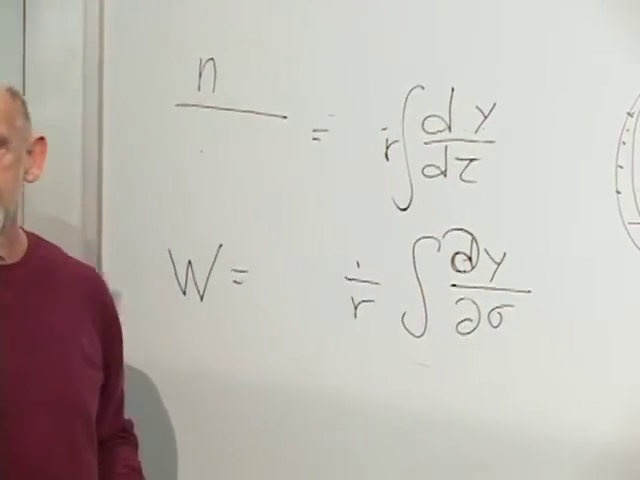
\includegraphics[width=0.72\textwidth]{lecture_10_figure_03.png}
  \medskip

  \begin{tikzpicture}[x=1cm,y=1cm,>=Latex]
    \draw[thick] (-4.0,0.3) circle (0.65);
    \draw[->,thick] (-4.55,0.58) arc (150:-145:0.65);
    \node at (-4.0,-0.65) {$w=+1$};
    \draw[thick] (-2.0,0.3) circle (0.65);
    \draw[->,thick] (-2.55,0.58) arc (150:-145:0.65);
    \node at (-2.0,-0.65) {$w=+1$};
    \node at (-3.0,0.3) {$+$};
    \draw[->,thick] (-1.0,0.3) -- (0.3,0.3);
    \draw[thick] (1.45,0.3) circle (0.78);
    \draw[thick] (1.45,0.3) circle (0.52);
    \draw[->,thick] (0.81,0.74) arc (145:-145:0.78);
    \node at (1.45,-0.78) {$w=+2$};
  \end{tikzpicture}
  \caption{같은 부호의 감김은 다시 연결되어 감김수가 두 배인 끈이 될 수 있다. 연결 상태는 달라져도 총 감김수 2는 유지된다.}
  \lectureframe{00:16:40}
  \label{fig:l10-same-winding}
\end{figure}

이 구분은 허용되는 모든 과정에서 유지된다. 총 감김수 100은 100번 감긴 끈 하나, 각각 50번 감긴 끈 두 개, 또는 한 번씩 감긴 끈 100개가 지닐 수 있다. 끈은 이 여러 형태 사이에서 갈라지고 합쳐질 수 있지만, 부호를 포함한 합은 계속 100이다. 이를 \(w\in\mathbb Z\)로 나타낸다.

\section{운동량 모드와 감김 모드}

보존만으로는 아직 쌍대성이 성립하는 것은 아니다. 다음으로 에너지를 비교해 보자. 콤팩트 원을 따라 움직이는 상태는 양자화된 운동량을 갖는다
\begin{equation}
  p_Y=\frac{n}{R},
  \qquad n\in\mathbb Z.
  \label{eq:l10-compact-momentum}
\end{equation}
다른 질량 기여를 무시할 수 있는 상태에서는 콤팩트 방향 운동이 \(E_{\rm mom}=|n|/R\)에 기여한다. \(n\)의 양수와 음수는 서로 반대 방향의 운동을 뜻하지만, 에너지는 양수다.

\begin{figure}[H]
  \centering
  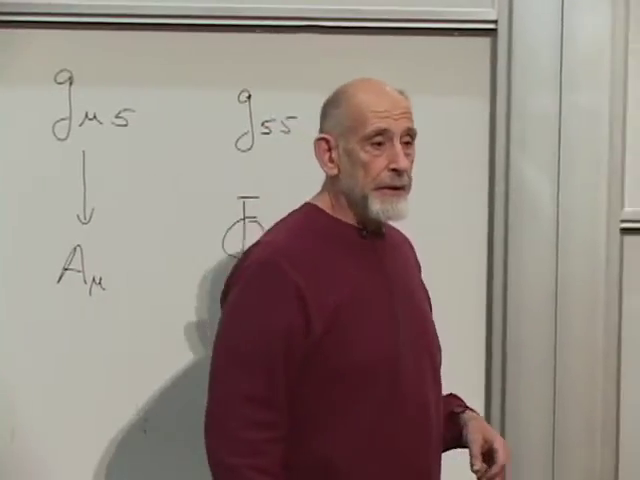
\includegraphics[width=0.72\textwidth]{lecture_10_figure_04.png}
  \caption{칠판에 적힌 콤팩트 운동량의 양자수. 강의에서는 운동량을 콤팩트 방향 속도의 적분으로 개략적으로 쓴다.}
  \lectureframe{00:21:30}
  \label{fig:l10-compact-momentum-board}
\end{figure}

\(|w|\)번 감긴 끈의 길이는 \(2\pi |w|R\)다. 기본 끈 장력을
\begin{equation}
  T_{\rm F}=\frac{1}{2\pi\alpha'},
\end{equation}
이라 하면, 감김 에너지는 다음과 같다.
\begin{equation}
  E_{\rm wind}=T_{\rm F}(2\pi |w|R)
  =\frac{|w|R}{\alpha'}.
  \label{eq:l10-winding-energy}
\end{equation}
강의에서 사용하는 단위계 \(\alpha'=1\)에서는 간단히 \(E_{\rm wind}=|w|R\)다.

반지름이 변할 때 두 에너지 탑은 서로 반대로 변한다. \(R\gg
\sqrt{\alpha'}\)이면 운동량 준위의 간격은 좁고 감김 준위의 간격은 넓다. \(R\ll\sqrt{\alpha'}\)이면 운동량 준위의 간격은 넓고 감김 준위의 간격은 좁다.

\begin{figure}[H]
  \centering
  \begin{minipage}[t]{0.48\textwidth}
    \centering
    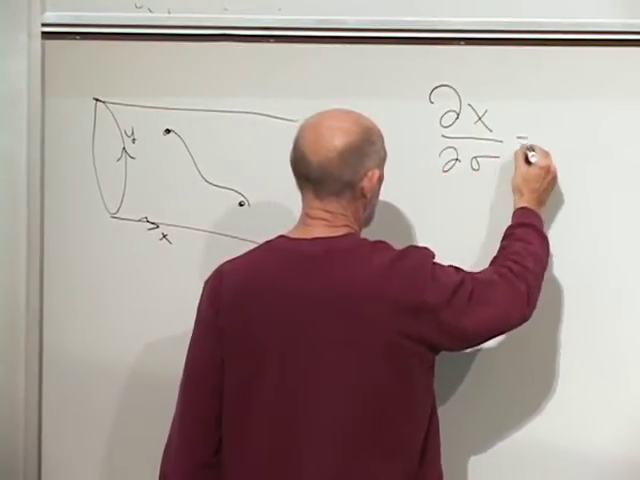
\includegraphics[width=\linewidth]{lecture_10_figure_05.png}
    \par\smallskip
    \textit{큰 콤팩트 반지름.}
  \end{minipage}\hfill
  \begin{minipage}[t]{0.48\textwidth}
    \centering
    \includegraphics[width=\linewidth]{lecture_10_figure_06.png}
    \par\smallskip
    \textit{작은 콤팩트 반지름.}
  \end{minipage}
  \caption{칠판에 나타난 두 스펙트럼을 비교한 그림. 반지름을 역수로 바꾸면 성긴 탑과 조밀한 탑의 역할이 서로 바뀐다.}
  \lectureframe{00:25:30--00:26:00}
  \label{fig:l10-dual-spectra-board}
\end{figure}

개략적인 관계는 다음과 같다.
\begin{figure}[H]
  \centering
  \begin{adjustbox}{max width=\linewidth}
  \begin{tikzpicture}[x=1cm,y=0.74cm,>=Latex]
    \node[font=\bfseries] at (-3.6,6.2) {$R\gg\sqrt{\alpha'}$};
    \draw[->] (-5.1,0) -- (-5.1,5.5) node[above] {$E$};
    \foreach \y in {0.4,1.0,1.6,2.2,2.8,3.4,4.0,4.6}
      \draw (-5.35,\y)--(-4.85,\y);
    \node[align=center] at (-4.25,5.15) {momentum\\dense};
    \draw[->] (-2.2,0) -- (-2.2,5.5) node[above] {$E$};
    \foreach \y in {0.4,2.4,4.4}
      \draw (-2.45,\y)--(-1.95,\y);
    \node[align=center] at (-1.35,5.15) {winding\\sparse};

    \node[font=\bfseries] at (3.6,6.2) {$R\ll\sqrt{\alpha'}$};
    \draw[->] (2.2,0) -- (2.2,5.5) node[above] {$E$};
    \foreach \y in {0.4,2.4,4.4}
      \draw (1.95,\y)--(2.45,\y);
    \node[align=center] at (3.05,5.15) {momentum\\sparse};
    \draw[->] (5.1,0) -- (5.1,5.5) node[above] {$E$};
    \foreach \y in {0.4,1.0,1.6,2.2,2.8,3.4,4.0,4.6}
      \draw (4.85,\y)--(5.35,\y);
    \node[align=center] at (5.95,5.15) {winding\\dense};
  \end{tikzpicture}
  \end{adjustbox}
  \caption{준위 간격 논증을 다시 그린 그림. 운동량과 감김을 서로 바꾸고 \(R\leftrightarrow\alpha'/R\)도 함께 바꾸어도 끈의 전체 스펙트럼은 변하지 않는다.}
  \label{fig:l10-dual-spectra-redraw}
\end{figure}

관찰자에게 이 스펙트럼 가운데 하나를 보여 주되 어떻게 얻었는지는 알려 주지 않았다고 하자. 간격이 좁은 탑은 큰 원 위의 운동량 탑일까, 작은 원 위의 감김 탑일까? 스펙트럼만으로는 알 수 없다. 끈 이론은 더 강한 주장을 한다. 산란 진폭으로도 둘을 구별할 수 없다는 것이다. 두 기술은 다음 변환 아래에서 정확히 동등하다.
\begin{equation}
  n\longleftrightarrow w,
  \qquad
  R\longleftrightarrow \widetilde R=\frac{\alpha'}{R}.
  \label{eq:l10-radius-duality}
\end{equation}
자기 자신으로 대응되는 고정점은
\begin{equation}
  R=\sqrt{\alpha'},
  \label{eq:l10-self-dual-radius}
\end{equation}
이며, 강의 단위계에서는 \(R=1\)다. 이 반지름에서는 추가 상태가 질량 없는 상태가 될 수 있고 게이지 대칭이 확장된다.

\begin{classroomqa}
\audiencequestion{감김은 스펙트럼을 다시 쓰기 위한 수학적 편의에 불과한가요? \lecturetimestamp{00:27:33}}
\lecturerresponse{아니다. 감김은 닫힌 끈 힐베르트 공간의 실제 부문을 나타내며, 이 부문들은 상호작용에 참여한다. ``이중성''이란 운동량 기술과 감김 기술이 동일한 물리의 서로 다른 좌표라는 뜻이다. 한 부문이 다른 부문을 대신해 선택적으로 쓰는 기억법이라는 뜻이 아니다.}
\end{classroomqa}

\begin{classroomqa}
\audiencequestion{자기 자신으로 대응되는 반지름이 있나요?
\lecturetimestamp{00:27:58}}
\lecturerresponse{있다. 자기이중 값은 \(R=\sqrt{\alpha'}\)이며, 칠판에서 사용한 단위계로는 \(R=1\)다. 이곳에서 두 탑이 만나고 스펙트럼의 대칭성이 확장된다.}
\end{classroomqa}

\section{이중성의 세계면 표현}

스펙트럼을 이용한 논증은 이중성을 시사하지만, 세계면을 보면 두 양의 교환을 더 정확히 나타낼 수 있다. 등각 게이지에서 \(Y\)에 켤레인 운동량은 \(\partial_\tau Y\)에 비례한다. 따라서 전체 콤팩트 운동량은 다음과 같다.
\begin{equation}
  P_Y=\frac{1}{2\pi\alpha'}
      \int_0^{2\pi}d\sigma\,\partial_\tau Y.
  \label{eq:l10-worldsheet-momentum}
\end{equation}
감김수는 다음과 같다.
\begin{equation}
  w=\frac{1}{2\pi R}
      \int_0^{2\pi}d\sigma\,\partial_\sigma Y
   =\frac{Y(2\pi)-Y(0)}{2\pi R}.
  \label{eq:l10-worldsheet-winding}
\end{equation}

\begin{classroomqa}
\audiencequestion{닫힌 끈을 따라 미분을 적분했는데도 왜 사라지지 않는가? \lecturetimestamp{00:32:33}}
\lecturerresponse{\(Y\)는 주기적인 표적 공간 좌표이지 \(\sigma\)-원 위에서 단일값을 갖는 실수 함수가 아니기 때문이다. 세계면의 점 \(\sigma=2\pi\)는 \(\sigma=0\)와 같은 점이지만, 매장을 덮개 직선 위로 올리면 \(2\pi wR\)만큼 변한다. \(\partial_\sigma Y\)의 적분은 그 이동량을 측정한다.}
\end{classroomqa}

\begin{figure}[H]
  \centering
  \includegraphics[width=0.76\textwidth]{lecture_10_figure_07.png}
  \caption{칠판에서 두 식을 모두 완성한 뒤의 운동량 적분과 감김 적분. 강의의 정규화에서는 공통 인자 \(2\pi\)와 \(\alpha'\)를 생략한다.}
  \lectureframe{00:33:25}
  \label{fig:l10-momentum-winding-integrals}
\end{figure}

한 번 감긴 끈의 경우,
\begin{equation}
  Y(\tau,\sigma+2\pi)=Y(\tau,\sigma)+2\pi R.
\end{equation}
감김수가 \(w\)이면 우변의 변위는 \(2\pi wR\)이다. 그러면 식 \eqref{eq:l10-worldsheet-winding}는 감김수를 정확히 센다. 이것이 칠판의 약식 표기 \(w\sim R^{-1}\int
d\sigma\,\partial_\sigma Y\)를 엄밀히 나타낸 것이다.

따라서 T-이중성의 세계면 표현은 다음과 같다.
\begin{equation}
  \partial_\tau Y\longleftrightarrow
  \partial_\sigma \widetilde Y,
  \qquad
  \partial_\sigma Y\longleftrightarrow
  \partial_\tau \widetilde Y,
  \label{eq:l10-derivative-duality}
\end{equation}
여기서는 \(Y\)의 운동량이 이중 좌표 \(\widetilde Y\)의 감김으로 바뀌며, 그 반대도 성립한다.

\begin{classroomqa}
\audiencequestion{그렇다면 세계면 좌표 \(\tau\)와 \(\sigma\) 자체가 서로 대응하거나 뒤바뀌나요?
\lecturetimestamp{00:34:39}}
\lecturerresponse{아니다. T-이중성은 해를 서로 대응시키고 콤팩트 표적 공간 좌표의 특정 미분을 교환한다. 세계면의 시간 좌표와 공간 좌표를 동일시하지 않는다.}
\end{classroomqa}

\section{감김 상태를 피할 수 없는 이유}

감기지 않은 상태가 있는데도 끈이 왜 감긴 상태로 나타나겠느냐고 물을 수 있다. 끈은 선호에 따라 상태를 선택하지 않는다. 충돌에서 공급된 에너지는 끈을 늘린다. 충분히 높은 에너지를 지닌 크게 변형된 끈은 서로 반대 방향으로 감긴 두 끈으로 다시 연결될 수 있다. 두 끈의 총 감김수는 여전히 0이지만, 분할 뒤에는 서로 멀어질 수 있다. 한 끈을 멀리 보내면 관찰자에게는 감긴 끈 하나만 고립되어 있는 듯 보일 수 있다.

\begin{figure}[H]
  \centering
  \includegraphics[width=0.76\textwidth]{lecture_10_figure_08.png}
  \caption{다시 연결된 뒤 서로 반대 방향으로 감긴 끈들이 분리될 수 있는, 크게 늘어난 총 감김수 0의 배치.}
  \lectureframe{00:36:15}
  \label{fig:l10-winding-pair-production}
\end{figure}

에너지 문턱은 감김 에너지로 정해진다. 큰 원에서는 콤팩트 방향을 충분히 감쌀 만큼 끈을 늘리려면 높은 충돌 에너지가 필요하다. 하지만 문턱을 넘으면 감김--반감김 쌍생성을 금지할 수 없다. 이는 광자 충돌로 전자--양전자가 생성되는 것과 비슷하다. 총 전하는 여전히 0이지만, 하전 입자들이 실제로 생겨 서로 떨어질 수 있다. 감김수 보존도 같은 방식으로 작동한다.

이 비유는 말뿐인 유사성이 아니다. 콤팩트 운동량과 감김은 서로 구별되는 두 전하 양자수처럼 작용한다. 이에 대응하는 저차원 기술에서 같은 부호끼리는 밀어내고 반대 부호끼리는 끌어당긴다. 그러므로 이 힘을 매개하는 두 벡터장을 찾아야 한다.

\section{5차원 중력에서 얻는 운동량 전하}

5차원 중력에서 시작하자. 대문자 첨자 \(M,N\)는 네 개의 보통 시공간 방향과 콤팩트한 다섯 번째 방향을 모두 가리킨다. 계량은 다음과 같이 분해된다.
\begin{equation}
  G_{MN}\quad\longrightarrow\quad
  \bigl\{G_{\mu\nu},\,G_{\mu5},\,G_{55}\bigr\}.
  \label{eq:l10-metric-decomposition}
\end{equation}
대칭성분 \(G_{5\mu}\)에는 \(G_{\mu5}\)에 이미 포함된 정보 외에 새로운 정보가 없다.

\begin{figure}[H]
  \centering
  \includegraphics[width=0.74\textwidth]{lecture_10_figure_09.png}
  \caption{서로 독립적인 5차원 계량 성분의 묶음: \(G_{\mu\nu}\), \(G_{\mu5}\), \(G_{55}\).}
  \lectureframe{00:44:05}
  \label{fig:l10-metric-components}
\end{figure}

4차원 관점에서 보면,
\begin{align}
  G_{\mu\nu} &\quad\hbox{is a spacetime metric},\\
  G_{\mu5} &\equiv A_\mu\quad\hbox{is a vector field},\\
  G_{55} &\equiv e^{2\varphi}\quad\hbox{is a scalar modulus}.
  \label{eq:l10-four-dimensional-fields}
\end{align}
스칼라 \(\varphi\)는 콤팩트 방향의 크기를 나타낸다. 이 값은 보통 시공간에 걸쳐 매끄럽게 변할 수 있으므로, \(\varphi\)의 파동은 다섯 번째 차원의 반지름이 요동하는 파동이다.

\begin{figure}[H]
  \centering
  \includegraphics[width=0.74\textwidth]{lecture_10_figure_10.png}
  \caption{칠판에서는 \(G_{\mu5}\)를 벡터 \(A_\mu\)와, \(G_{55}\)을 스칼라 \(\Phi\)와 대응시킨다.}
  \lectureframe{00:47:40}
  \label{fig:l10-vector-and-radius-modulus}
\end{figure}

혼합 중력 성분의 원천은 혼합 운동량 흐름이다. 특히 다섯 번째 방향을 따른 운동량은 \(G_{\mu5}\)의 원천이 된다. 따라서 4차원 관찰자는 정수 \(n\)를 \(A_\mu\)에 결합하는 전하로 해석한다. 이것이 칼루차--클라인 메커니즘이다. 고차원 기하에서 운동량이던 것이 저차원 장 이론에서는 전하가 된다.

\editorialnote{\(G_{55}\)에서 나온 스칼라를 강의에서는 느슨하게 ``딜라톤''이라고 부른다. 이 축약에서 이 스칼라는 구체적으로 반지름 모듈러스다. 끈 결합을 조절하는 10차원 끈 딜라톤은 별개의 장이지만, 기준계와 이중성을 바꾸면 저차원 스칼라의 조합들이 서로 섞일 수 있다.}

\begin{classroomqa}
\audiencequestion{스칼라 \(\varphi\)는 운동량 정수 \(n\)에 비례하나요? \lecturetimestamp{00:48:43}}
\lecturerresponse{아니다. 정수 \(n\)는 양자화된 상태를 표시하고 전하로 작용한다. 스칼라 \(\varphi(x)\)는 콤팩트화의 국소적 크기를 정하는 연속장이다. 위치에 따라 달라질 수 있으며, 그 자체가 정수인 것은 아니다.}
\end{classroomqa}

\section{두 번째 벡터장과 감김 전하}

감김도 전하와 비슷한 양이지만, 같은 벡터장에 같은 방식으로 결합할 수는 없다. 두 번째 벡터장을 보려면 최초의 닫힌 끈 들뜸으로 돌아가자. 닫힌 끈에는 왼쪽 진행 진동 모드와 오른쪽 진행 진동 모드가 있다. 물리적 상태는 레벨 정합 조건을 만족해야 한다. 즉 왼쪽 진행과 오른쪽 진행의 총 들뜸 준위가 서로 같아야 한다.

보손 이론에서 들뜸이 없는 상태는 타키온이다. 왼쪽 진행 또는 오른쪽 진행 진동자 하나만 들뜨면 레벨 정합을 어긴다. 따라서 처음으로 허용되는 질량 없는 상태에는 각 종류의 진동자가 하나씩 포함된다.
\begin{equation}
  \alpha_{-1}^{I}\widetilde\alpha_{-1}^{J}\ket{0;k}.
  \label{eq:l10-first-massless-state}
\end{equation}
첨자 \(I,J\)는 콤팩트 방향을 포함하는 횡방향 공간 성분을 가리킨다. 한 첨자는 보통 방향을, 다른 첨자는 \(5\)를 가리키면 벡터형 진동자 상태 두 개가 생긴다.
\begin{equation}
  \alpha_{-1}^{\mu}\widetilde\alpha_{-1}^{5}\ket{0;k},
  \qquad
  \alpha_{-1}^{5}\widetilde\alpha_{-1}^{\mu}\ket{0;k}.
  \label{eq:l10-two-vector-states}
\end{equation}

\begin{figure}[H]
  \centering
  \includegraphics[width=0.76\textwidth]{lecture_10_figure_11.png}
  \caption{왼쪽--오른쪽 진동자의 두 배열 순서. 편광 가운데 하나가 콤팩트 방향을 가리키면 4차원 벡터 상태가 된다.}
  \lectureframe{00:58:20}
  \label{fig:l10-two-vector-states-board}
\end{figure}

대칭 조합과 반대칭 조합은 서로 다른 시공간 장에 속한다.
\begin{align}
  \alpha_{-1}^{(\mu}\widetilde\alpha_{-1}^{5)}\ket{0;k}
    &\longleftrightarrow G_{\mu5},\\
  \alpha_{-1}^{[\mu}\widetilde\alpha_{-1}^{5]}\ket{0;k}
    &\longleftrightarrow B_{\mu5}.
  \label{eq:l10-g-and-b-vectors}
\end{align}
첫 번째는 콤팩트 운동량이 원천인 칼루차--클라인 벡터다. 두 번째는 반대칭 칼브--라몽 장에서 유래하며 끈 감김이 원천이다. 따라서 축약된 이론에는 각 전하 부문에 하나씩, 광자와 비슷한 장 두 개가 들어 있다.

두 진동자 첨자가 모두 콤팩트 방향을 가리키면 그 상태는 콤팩트화 모듈러스에 대응하는 스칼라다. 두 첨자가 모두 보통 횡방향을 가리키면 대칭 무대각합 성분은 중력자이고, 반대칭 성분은 \(B_{\mu\nu}\)이며, 대각합 성분은 스칼라 부문에 기여한다.

\begin{classroomqa}
\audiencequestion{이 상태 가운데 어느 것이 단일항이고 어느 것이 삼중항인가요? \lecturetimestamp{01:00:21}}
\lecturerresponse{여기서는 그 분류가 유용하지 않다. 혼합 상태 두 개 모두 4차원 벡터로 변환된다. 이들의 합과 차는 계량의 대칭 편광과 반대칭 \(B\)장 편광을 분리한다. 콤팩트 첨자 두 개를 지닌 상태는 4차원 스칼라다.}
\end{classroomqa}

휴식 전에 도달한 전체 대응 관계는 다음과 같다.
\begin{equation}
  \boxed{
  \begin{gathered}
    n\leftrightarrow w,
    \qquad
    R\leftrightarrow\dfrac{\alpha'}{R},\\
    \partial_\tau Y\leftrightarrow\partial_\sigma\widetilde Y,
    \qquad
    G_{\mu5}\leftrightarrow B_{\mu5}.
  \end{gathered}}
  \label{eq:l10-complete-t-duality-map}
\end{equation}

\begin{figure}[H]
  \centering
  \includegraphics[width=0.72\textwidth]{lecture_10_figure_12.png}
  \caption{칠판에 정리한 T-이중성 사상: 운동량과 감김, 반지름과 역수 반지름, 세계면 미분, 두 벡터장이 서로 교환된다. 강의자는 마지막 줄 일부를 가리므로 식 \eqref{eq:l10-complete-t-duality-map}에 그 내용을 명시했다.}
  \lectureframe{01:02:20}
  \label{fig:l10-t-duality-map-board}
\end{figure}

이 구성을 지금까지 나열한 모든 장이 관측된 입자 스펙트럼에서 이미 확인되었다는 주장과 혼동해서는 안 된다. 여기까지는 콤팩트화된 끈 이론의 수학적 귀결이다. 이러한 구조를 현상론과 연결하려는 제안은 많지만, 이 강의에서 풀려는 문제는 아니다.

\section{열린 끈은 질문을 바꾼다}

휴식 뒤에는 열린 끈에서 다시 시작한다. 닫힌 끈에는 감김이 빠져나갈 끝점이 없으므로 안정된 감김 상태가 가능하다. 열린 끈에는 끝점이 있어 이와 비슷하게 위상적으로 보호되는 감김수가 없다. 그런데도 T-이중성은 이론의 정확한 대칭이다. 열린 끈에 이 대칭은 어떤 작용을 할까?

자유롭게 움직이는 끝점의 경우, 끈 작용을 변분하면 노이만 경계 조건이 나온다. 단순한 \((X,Y)\) 기하에서는
\begin{equation}
  \left.\partial_\sigma X\right|_{\partial\Sigma}=0,
  \qquad
  \left.\partial_\sigma Y\right|_{\partial\Sigma}=0.
  \label{eq:l10-neumann-boundary}
\end{equation}
역학적 그림은 간단하다. 끈을 질량이 점점 작아지는 요소들이 이어진 사슬로 보자. 마지막 요소에 접선 방향의 힘이 작용하면 질량이 한없이 작아질수록 그 요소의 가속도는 발산한다. 따라서 자유 끝점은 끝점의 알짜 장력이 사라지도록 위치를 조정한다. 누군가 끝점을 고정하고 필요한 힘을 가할 수도 있지만, 그러면 끝점은 더 이상 자유롭지 않다.

\begin{figure}[H]
  \centering
  \includegraphics[width=0.76\textwidth]{lecture_10_figure_13.png}
  \caption{완성한 노이만 끝점 조건을 표시한 열린 끈: \(\partial_\sigma X=\partial_\sigma Y=0\).}
  \lectureframe{01:09:20}
  \label{fig:l10-neumann-board}
\end{figure}

이제 콤팩트 좌표 \(Y\)에만 이중성 변환을 적용하자. 비콤팩트 좌표 \(X\)는 그대로 둔다. 식 \eqref{eq:l10-derivative-duality}에 따라 두 번째 노이만 조건은 다음과 같이 바뀐다.
\begin{equation}
  \left.\partial_\tau\widetilde Y\right|_{\partial\Sigma}=0.
  \label{eq:l10-dirichlet-time-derivative}
\end{equation}
따라서 이중화된 콤팩트 방향에서 끝점의 위치는 시간에 따라 변하지 않는다.
\begin{equation}
  \left.\widetilde Y\right|_{\partial\Sigma}=Y_0.
  \label{eq:l10-dirichlet-boundary}
\end{equation}
이것이 디리클레 경계 조건이다.

\begin{figure}[H]
  \centering
  \includegraphics[width=0.76\textwidth]{lecture_10_figure_14.png}
  \medskip

  \begin{adjustbox}{max width=\linewidth}
  \begin{tikzpicture}[x=1cm,y=1cm,>=Latex]
    \node[align=center] at (-3.5,0.8)
      {Neumann\\\(\left.\partial_\sigma Y\right|_{\partial\Sigma}=0\)};
    \draw[->,thick] (-1.7,0.8) -- (1.3,0.8)
      node[midway,above] {$T_Y$};
    \node[align=center] at (3.4,0.8)
      {Dirichlet\\\(\left.\partial_\tau\widetilde Y\right|_{\partial\Sigma}=0\)};
    \node[align=center] at (3.4,-0.5)
      {\(\widetilde Y(\tau)=Y_0\) at each endpoint};
  \end{tikzpicture}
  \end{adjustbox}
  \caption{칠판에 적힌 완성된 이중 끝점 조건과 그 논리의 깔끔한 재구성. T-이중성은 콤팩트 방향의 자유로운 움직임을 이중 방향에서의 고정된 끝점 위치로 바꾼다.}
  \lectureframe{01:12:35}
  \label{fig:l10-neumann-to-dirichlet}
\end{figure}

\begin{classroomqa}
\audiencequestion{이중화된 조건은 왜 끝점이 고정되었다는 뜻인가요? \lecturetimestamp{01:12:39}}
\lecturerresponse{\(\partial_\tau\widetilde Y=0\)가 이중화된 방향의 속도가 0이라는 뜻이기 때문이다. 끝점은 \(\widetilde Y\)의 어느 위치에서 시작하든 계속 그 자리에 머문다. 이중화하지 않은 방향에 평행한 좌표는 여전히 자유롭다.}
\end{classroomqa}

\section{끝점을 붙드는 대상은 D-브레인이다}

끝점이 고정되어 있다면 그 자리에 붙들어 둘 무언가가 있어야 한다. 따라서 정확한 T-이중성을 위해서는 열린 끈이 끝날 수 있는 새로운 대상이 필요하다. 그것이 D-브레인이다. 문자 \(D\)는 대상의 차원이 아니라 디리클레를 뜻한다. 강의의 역사적 일화에 따르면 이 대상은 조지프 폴친스키의 이름을 따서 불렸을 수도 있다. 그의 분석이 그 동역학적 역할을 분명히 드러냈기 때문이다. 하지만 이미 쓰이고 있던 용어 ``p-브레인'' 때문에 디리클레가 자연스러운 이름으로 남았다.

\(p\)-브레인은 공간 차원이 \(p\)개인 대상이다. 끈은 1-브레인, 막은 2-브레인이며, 3차원으로 뻗은 대상은 3-브레인이다. D\(p\)-브레인은 횡방향에서 기본 끈의 끝점이 디리클레 조건을 따르고 브레인에 접한 방향에서는 노이만 조건을 따르는 \(p\)-브레인이다.

이중성 논증은 \(Y_0\)의 특정 값을 특별히 택하지 않으므로, D-브레인은 우주의 한 지점에 못 박힌 고정 장치일 수 없다. 움직일 수 있어야 한다. 상대성 이론은 절대적으로 강체인 확장된 물체도 허용하지 않으므로 D-브레인은 요동치고 휘어질 수 있다. 칠판에 그린 단순한 평탄 브레인은 평형 배치일 뿐, 동역학을 제한하는 조건이 아니다.

\begin{classroomqa}
\audiencequestion{열린 끈의 두 끝점은 쌍대 좌표의 같은 고정값을 가져야 하나요? \lecturetimestamp{01:14:55}}
\lecturerresponse{일반적으로 그렇지는 않다. 두 끝점이 같은 D-브레인 위에 있을 수 있으며, 이 경우 두 끝점은 그 브레인의 횡방향 위치를 공유한다. 서로 다른 횡방향 위치에 있는 두 D-브레인에 각각 놓일 수도 있으며, 그러면 끈은 그 사이에 걸쳐 있다. 브레인 자체도 요동하고 휘어질 수 있으므로, 끝점의 궤적이 완전히 평평한 평면에 계속 놓여 있을 필요는 없다.}
\end{classroomqa}

\section{D-브레인의 차원 세기}

10차원 초끈 이론에는 9개의 공간 차원이 있다. T-이중성이 한 공간 방향에 디리클레 조건을 부과한다고 하자. 끝점은 나머지 8개 방향에서는 여전히 자유로우므로, 끝점이 놓일 수 있는 자취는 8차원 D8-브레인이다. 서로 독립인 디리클레 조건을 하나 더 부과할 때마다 끝점의 운동 방향이 하나씩 줄어든다. 공간 좌표 \(k\)개를 고정하면
\begin{equation}
  p=9-k.
  \label{eq:l10-dp-counting}
\end{equation}

탁자 위에서 같은 차원 계산의 3차원 사례를 볼 수 있다. 수직 좌표를 고정하면 손가락 끝은 2차원 탁자 위에서 움직일 수 있다. 두 번째 좌표도 고정하면 선을 따라 움직일 수 있다. 세 좌표를 모두 고정하면 한 점에 갇힌다.

\begin{figure}[H]
  \centering
  \begin{adjustbox}{max width=\linewidth}
  \begin{tikzpicture}[x=1.05cm,y=1cm,>=Latex]
    \draw[fill=blue!8] (-5.5,-0.7) -- (-2.5,-0.7) -- (-1.7,0.2)
      -- (-4.7,0.2) -- cycle;
    \node at (-3.6,-1.15) {one constraint: sheet};
    \draw[very thick,blue!60!black] (-0.9,-0.25) -- (1.3,-0.25);
    \node at (0.2,-1.15) {two constraints: line};
    \fill[blue!70!black] (4.1,-0.25) circle (0.09);
    \node at (4.1,-1.15) {three constraints: point};
    \draw[->] (-1.45,0.95) -- (-0.75,0.95);
    \draw[->] (2.25,0.95) -- (2.95,0.95);
    \node at (0.35,1.35) {each Dirichlet condition lowers \(p\) by one};
  \end{tikzpicture}
  \end{adjustbox}
  \caption{탁자 위에서 설명한 차원 계산 논증. D\(p\)-브레인은 끝점이 자유롭게 움직일 수 있는 자취다.}
  \label{fig:l10-dp-counting-redraw}
\end{figure}

반복해서 이중성 변환을 적용하면 D8-, D7-, D6-브레인 등이 생기며, 공간에서 점처럼 보이는 D0-브레인까지 이어진다. 고정된 공간 방향이 하나도 없으면 D9-브레인이 아홉 공간 차원을 모두 채우므로 보통의 열린 끈은 어디서나 자유롭게 움직인다. 강의에서는 D\((-1)\)-브레인도 잠시 언급한다. 이들은 유클리드 시공간에 국소화되어 있으며, 시간에 따라 전파되는 보통 입자가 아니라 순간자로 작용한다.

\editorialnote{차원 사다리는 IIA형과 IIB형 이론을 함께 놓고 볼 때 성립한다. 안정한 BPS D\(p\)-브레인은 IIA형에서 짝수 \(p\)를, IIB형에서 홀수 \(p\)를 갖는다. 한 원을 따라 T-이중성을 적용하면 \(p\)가 하나 바뀌는 동시에 IIA형 이론과 IIB형 이론이 서로 바뀐다.}

\begin{classroomqa}
\audiencequestion{콤팩트한 차원이 여섯 개뿐이라면, 세는 일은 아홉이 아니라 여섯에서 빼는 것으로 시작해야 하나요? \lecturetimestamp{01:20:49}}
\lecturerresponse{기본적인 유도에서는 콤팩트 방향에 T-쌍대성을 적용하지만, 원래 원이 작아질수록 쌍대 원은 임의로 커진다. 그 극한에서는 사실상 비콤팩트하다. 따라서 결과로 생기는 브레인은 접근 가능한 규모에서 비콤팩트하게 보이는 방향을 따라 뻗거나 그런 방향에 수직일 수 있다. 차원 \(p\)는 한 유도에서 사용한 콤팩트 방향만이 아니라 브레인에 접하는 모든 공간 방향을 센다.}
\end{classroomqa}

D0-브레인은 새로운 종류의 입자다. 열린 끈은 한 D0-브레인에서 다른 브레인으로 이어지거나, 같은 D0-브레인으로 되돌아오거나, 아주 멀리 떨어진 브레인까지 뻗을 수 있다. 끈의 다른 끝점을 문자 그대로 공간 무한대에 두면 길이가 무한하고 따라서 에너지도 무한하다. 그러므로 물리적으로 유용한 설정에서는 다른 끝점을 또 다른 대상에 놓는다.

다음 사례인 D1-브레인도 끈 모양이지만, 우리가 처음 살펴본 기본 끈과는 다르다. 휘어질 수 있고 자기 자신과 이어져 닫힌 형태를 이룰 수도 있으며, 기본 끈은 그 위에서 끝날 수 있다. 그 장력은 끈 결합상수에 따라 다른 방식으로 변한다:
\begin{equation}
  T_{\rm D1}=\frac{1}{2\pi\alpha' g_s},
  \qquad
  T_{\rm F1}=\frac{1}{2\pi\alpha'}.
  \label{eq:l10-dstring-tension}
\end{equation}
결합이 약한 \(g_s\ll1\)에서는 D-끈이 기본 끈보다 훨씬 무겁다. 그래서 처음에는 무거운 닻처럼 나타난다.

\begin{figure}[H]
  \centering
  \includegraphics[width=0.76\textwidth]{lecture_10_figure_15.png}
  \caption{칠판에 그린 D1-브레인: 휘어질 수 있는 일차원 물체로, 기본 끈과는 구별되며 기본 끈은 그 위에서 끝날 수 있다.}
  \lectureframe{01:24:20}
  \label{fig:l10-d1-brane}
\end{figure}

\begin{classroomqa}
\audiencequestion{T-이중성은 끈뿐 아니라 D-브레인에도 작용하나요? \lecturetimestamp{01:25:35}}
\lecturerresponse{그렇다. D\(p\)-브레인에 평행한 방향으로 T-이중성을 적용하면 차원이 D\((p-1)\)로 낮아지고, 브레인에 수직인 방향으로 적용하면 차원이 D\((p+1)\)로 높아진다. 브레인은 이중성 사전의 일부이며, 이중성에 영향을 받지 않은 채 그대로 남는 외부 지지체가 아니다.}
\end{classroomqa}

\begin{classroomqa}
\audiencequestion{브레인에 접하는 방향도 여전히 콤팩트할 수 있나요?
\lecturetimestamp{01:27:25}}
\lecturerresponse{그렇다. ``접함''과 ``콤팩트함''은 서로 다른 질문에 답한다. 어떤 방향은 브레인을 따라 놓이면서도 원을 이루어 닫힐 수 있고, 비콤팩트할 수도 있다. 끝점에 중요한 것은 그 방향의 경계 조건이 노이만인지 디리클레인지 여부다.}
\end{classroomqa}

D2-브레인은 막과 비슷한 면이다. D3-브레인에는 공간 차원이 세 개 있다. 실제로 더 높은 차원의 시공간에서는 D3-브레인이 공간 전체가 아니라 삼차원 부분공간이다. 비록 그 안에 갇힌 관측자에게는 그곳이 공간 전체처럼 느껴질 수 있지만 말이다.

\begin{figure}[H]
  \centering
  \includegraphics[width=0.76\textwidth]{lecture_10_figure_16.png}
  \caption{끈의 끝점이 움직일 수 있는 면으로 그린 D2-브레인.}
  \lectureframe{01:27:55}
  \label{fig:l10-d2-brane}
\end{figure}

여기서 제시한 유도는 의도적으로 개략적인 설명에 그친다. 이것만으로 끈 이론이 자연을 기술한다는 사실이 증명되는 것은 아니다. 그러나 끈 이론 안에서는 이중성, 양자 계산, 수학적 결과 등 일관성을 확인하는 근거가 많으며, 이들은 모두 D-브레인이 실제로 동역학을 따르는 물체임을 가리킨다.

\section{브레인 위에서 장이 되는 열린 끈}

다른 것은 비어 있는 D2-브레인 위에 짧은 열린 끈들을 놓아 보자. 각 끝점은 면에 갇혀 있으므로 저에너지 들뜸 전체가 면을 따라 움직인다. 인접한 끝점의 화살표 방향이 서로 맞는 두 개의 방향이 정해진 끈은 이어 붙을 수 있다. 이어진 끈은 나중에 다시 갈라질 수 있다. 이를 입자의 역사로 읽으면 파인만 도표의 꼭짓점에 해당한다. 입자 두 개가 들어오고, 중간 들뜸이 전파된 뒤, 입자 두 개가 나온다.

\begin{figure}[H]
  \centering
  \includegraphics[width=0.76\textwidth]{lecture_10_figure_17.png}
  \caption{방향이 정해진 열린 끈들이 D2-브레인 위에서 끝점의 방향이 서로 맞아 이어지고 있다. 저에너지에서는 이 과정이 브레인 위의 장론 상호작용으로 해석된다.}
  \lectureframe{01:29:55}
  \label{fig:l10-open-strings-on-brane}
\end{figure}

끈의 에너지 척도보다 훨씬 낮은 에너지에서는 내부 진동 탑이 들뜨지 않는다. 남는 질량 없는 열린 끈 상태는 브레인의 월드볼륨 위에 놓인 벡터장이다. 브레인이 하나라면 이는 아벨 게이지 장 \(U(1)\)이며, 전자기장에 해당하는 브레인상의 장이다. 이 장은 10차원 벌크 전체에 걸쳐 전파되지 않는다. 그 양자는 끝점이 브레인에 머물게 하는 열린 끈이다.

\section{브레인 다발은 비아벨 색을 만든다}

이제 서로 가까이 있는 평행한 브레인 여러 개를 놓아 보자. 브레인이 세 개라면 각각을 빨강, 초록, 파랑으로 표시하자. 방향이 정해진 끈에는 끝점의 표지 두 개가 순서대로 붙는다. 예를 들어 빨강에서 초록으로, 초록에서 파랑으로, 빨강에서 빨강으로 이어질 수 있다. 브레인이 \(N\)개일 때 질량 없는 열린 끈 상태는 \(N\times N\) 행렬로 배열할 수 있다.
\begin{equation}
  A_\mu{}^{i}{}_{j},
  \qquad i,j=1,\ldots,N.
  \label{eq:l10-chan-paton-matrix}
\end{equation}
이 표지들은 ---패턴 라벨이며, \(U(N)\) 게이지 이론을 이룬다.

\begin{figure}[H]
  \centering
  \includegraphics[width=0.76\textwidth]{lecture_10_figure_18.png}
  \medskip

  \begin{adjustbox}{max width=\linewidth}
  \begin{tikzpicture}[x=1cm,y=1cm,>=Latex]
    \draw[very thick,red!70!black] (-4.8,2.0)--(4.8,2.0);
    \draw[very thick,green!55!black] (-4.8,0.8)--(4.8,0.8);
    \draw[very thick,blue!70!black] (-4.8,-0.4)--(4.8,-0.4);
    \node[left] at (-4.8,2.0) {Red};
    \node[left] at (-4.8,0.8) {Green};
    \node[left] at (-4.8,-0.4) {Blue};
    \draw[->,thick] (-3.4,2.0) .. controls (-2.8,1.35) and (-2.3,1.15)
      .. (-1.7,0.8);
    \node at (-2.7,1.05) {$R\!G$};
    \draw[->,thick] (-0.6,0.8) .. controls (0.0,0.25) and (0.6,-0.05)
      .. (1.2,-0.4);
    \node at (0.1,0.0) {$G\!B$};
    \draw[->,thick] (2.1,2.0) .. controls (2.9,2.55) and (3.8,2.55)
      .. (4.3,2.0);
    \node at (3.2,2.65) {$R\!R$};
  \end{tikzpicture}
  \end{adjustbox}
  \caption{칠판의 평행한 브레인 세 개와, 그 사이를 잇는 끈이 지닌 순서 있는 끝점 표지를 깔끔하게 재구성한 그림.}
  \lectureframe{01:33:15}
  \label{fig:l10-three-brane-stack}
\end{figure}

\begin{classroomqa}
\audiencequestion{끈이 다른 그림에 막히지 않고 빨강 브레인에서 초록 브레인까지 실제로 이어질 수 있나요? \lecturetimestamp{01:35:07}}
\lecturerresponse{그렇다. 브레인은 더 높은 차원의 공간에 놓여 있다. 칠판의 이차원 그림은 투영에 불과하므로, 끈은 수직 방향으로 움직여 투영된 다른 선을 돌아갈 수 있다.}
\end{classroomqa}

\begin{classroomqa}
\audiencequestion{빨강--초록 끈이 빨강--파랑 끈이 되려면 초록--파랑 끈과 합쳐져야 하나요? \lecturetimestamp{01:35:39}}
\lecturerresponse{그것이 기본적인 국소 접합 규칙이다. 서로 맞는 끝점들이 만나고, 두 선분은 하나의 끈이 된다. 이어지지 않은 양 끝점에는 빨강과 파랑이라는 표지가 그대로 남는다. 더 복잡한 과정도 같은 연산을 반복해 구성할 수 있다.}
\end{classroomqa}

결합 규칙은 행렬 곱셈을 기하학적으로 나타낸 것이다. 빨강--초록 끈은 한쪽의 초록 끝점이 다른 쪽의 초록 끝점과 맞으므로 초록--파랑 끈과 결합할 수 있다. 그 결과는 빨강--파랑 끈이다:
\begin{equation}
  (R,G)\circ(G,B)\longrightarrow(R,B).
  \label{eq:l10-color-composition}
\end{equation}
반복되는 인덱스는 서로 연결되어 내부에서 사라진다. 이는 양--밀스 상호작용 꼭짓점에 나타나는 것과 같은 인덱스 구조다.

\begin{figure}[H]
  \centering
  \includegraphics[width=0.76\textwidth]{lecture_10_figure_19.png}
  \caption{브레인 다발 위에서 열린 끈들이 이어지고 있다. 끝점의 방향은 비아벨 게이지 장에서 쓰는 순서 있는 지수의 합성과 같은 규칙을 강제한다.}
  \lectureframe{01:36:30}
  \label{fig:l10-color-joining-board}
\end{figure}

일치하는 브레인 세 개의 열린 끈 게이지 군은 \(U(3)\)이며 벡터 상태 아홉 개를 갖는다. 그 대수는 다음과 같이 분해된다.
\begin{equation}
  \mathfrak u(3)=\mathfrak{su}(3)\oplus\mathfrak u(1).
  \label{eq:l10-u3-decomposition}
\end{equation}
무대각 성분 여덟 개는 QCD 글루온의 색 구조를 이룬다. 반면 대각 성분인 질량중심 \(U(1)\)는 별도의 아벨 장이다.

\editorialnote{강의에서는 아홉 가지 색 쌍 조합 가운데 하나가 떨어져 나가 사라질 수 있어 글루온 여덟 개만 남는다고 설명한다. D-브레인에 관한 정확한 진술은 서로 일치하는 브레인 세 개의 다발이 \(U(3)\)를 준다는 것이며, \(SU(3)\)만 주는 것이 아니다. QCD의 옥텟을 얻으려면 대각 성분인 \(U(1)\)를 분리하거나, 사영으로 제거하거나, 그 밖의 방법으로 동역학에서 분리해야 한다. 강의의 그림은 순서가 있는 색 지수를 이해하는 데 도움이 되지만, QCD를 완전히 유도한 것은 아니다.}

쿼크와 같은 물질은 색 지수를 하나만 가진다. 브레인 그림에서는 한쪽 끝이 색 브레인 다발에, 다른 쪽 끝이 멀리 떨어진 다른 브레인에 놓인 끈으로 나타낸다. 색 브레인 다발을 기준으로 보면 한쪽 끝만 색 표지로 드러난다. 방향을 뒤집으면 반입자가 된다. 쿼크형 끈과 반쿼크형 끈은 끝점이 서로 맞으면 이어져 색 브레인 다발에서 떨어져 나갈 수 있다. 같은 방향을 가진 쿼크형 끈 두 개는 그런 방식으로 소멸할 수 없다.

그 결과 얻는 이론은 일반적으로 초대칭 양--밀스 이론이며, 추가 물질의 종류는 브레인과 그 교차에 따라 정해진다. 비아벨 동역학을 밝히는 데 도움이 될 만큼 QCD와 가깝지만, 저절로 표준 모형이 되는 것은 아니다. 브레인이 하나일 때 같은 구성은 \(U(1)\) 이론으로 줄어든다. 짧은 브레인--브레인 끈은 광자와 같은 역할을 하고, 두 번째 부문까지 뻗는 방향이 정해진 끈은 양전하와 음전하의 역할을 한다.

\section{자기 홀극으로 끝나는 D-끈}

이제 이야기에는 끈 모양의 물체가 두 종류 있다. 원래의 기본 끈, 즉 F-끈은 D3-브레인 위에서 전기 플럭스를 운반한다. D1-브레인, 즉 D-끈은 결합이 약할 때 훨씬 더 무겁다. D-끈도 D3-브레인 위에서 끝날 수 있다. 그 끝점은 월드볼륨 게이지 장에 대한 전하를 띠지 않는다. 대신 자기 전하를 띤다. D3-브레인 위의 관측자에게 그 끝점은 자기 홀극이다.

\begin{figure}[H]
  \centering
  \includegraphics[width=0.76\textwidth]{lecture_10_figure_20.png}
  \medskip

  \begin{adjustbox}{max width=\linewidth}
  \begin{tikzpicture}[x=1cm,y=1cm,>=Latex]
    \draw[fill=blue!7] (-3.8,-0.5)--(2.6,-0.5)--(3.6,0.35)--(-2.8,0.35)--cycle;
    \node at (2.25,-0.95) {D3-brane};
    \draw[very thick,red!70!black] (0.0,3.0)--(0.0,0.0);
    \fill[black] (0.0,0.0) circle (0.08);
    \node[right] at (0.15,2.1) {D-string};
    \foreach \a in {25,65,115,155} {
      \draw[->,blue!65!black] (0.0,0.0)--({1.25*cos(\a)},{0.65*sin(\a)});
    }
    \node[align=center] at (4.8,1.7) {magnetic flux\\on the D3 worldvolume};
    \draw[->] (3.7,1.35)--(1.05,0.45);
  \end{tikzpicture}
  \end{adjustbox}
  \caption{보드 끝점 구성과 그 명료한 해석. D끈이 D3-브레인에 끝나는 경우, 월드볼륨 게이지 이론에서는 자기 홀극으로 나타난다.}
  \lectureframe{01:41:30}
  \label{fig:l10-dstring-monopole}
\end{figure}

질량의 계층도 정성적으로 올바른 형태를 갖는다. D-끈의 장력에는 \(1/g_s\) 인자가 들어가므로, 결합이 약할 때 그 끝점은 보통의 전기적 들뜸보다 훨씬 무겁다. F-끈과 D-끈 끝점 사이의 전기·자기 관계는 IIB형 끈 이론의 더 넓은 이중성 구조에 속한다.

\begin{classroomqa}
\audiencequestion{D-끈의 끝점은 중성인가요?
\lecturetimestamp{01:42:19}}
\lecturerresponse{기본 끈 끝점이 띠는 전기 전하에 대해서는 중성이지만, 전하가 없는 것은 아니다. 자기 전하를 띠므로 D3-브레인 게이지 이론에서 홀극이다.}
\end{classroomqa}

\section{이 구성이 주장하는 것과 주장하지 않는 것}

T-이중성에서 브레인으로 이어지는 흐름은 한 번의 계산으로 완성된 것이 아니라 수십 년에 걸쳐 구축되었다. 강입자를 기술하기 위해 처음 제안된 이론은 양자 중력의 후보 이론이 되었다. 뒤이어 이중성 때문에 D-브레인이 이론의 스펙트럼에 포함되었고, 브레인에서 끝나는 끈의 저에너지 동역학으로 게이지 이론이 다시 등장했다. 그런 의미에서 이 주제는 한 바퀴를 돌아 제자리로 왔다.

D-브레인과 관련된 이중성 구성은 초대칭 게이지 이론, 강결합 계, 중력과 장론 사이의 관계를 연구하는 강력한 도구가 되었다. 게이지/중력 이중성을 통해 유체와 플라스마 모형에도 통찰을 제공했다. 그러나 이러한 성과가 관측된 입자 스펙트럼을 직접 유도했다는 뜻은 아니다. 콤팩트화 기하, 브레인 배치, 초대칭 깨짐을 비롯한 여러 요소를 여전히 선택해야 한다.

\begin{classroomqa}
\audiencequestion{어떤 콤팩트 차원을 이중화할지는 무엇으로 정해지나요?
\lecturetimestamp{01:44:59}}
\lecturerresponse{수학적으로는 필요한 대칭성이 있는 콤팩트 방향이라면 어느 것이든 이중화할 수 있으며, 가장 편리한 기술을 선택하면 된다. 물리적으로는 특정 상태에서 실현되는 브레인의 방향과 콤팩트화 자료가 그 상태의 역사와 동역학에 따라 정해진다.}
\end{classroomqa}

\begin{classroomqa}
\audiencequestion{홀극 구성에는 어떤 브레인이 필요한가요?
\lecturetimestamp{01:45:21}}
\lecturerresponse{게이지 이론이 경험하는 세계는 D3-브레인이다. D-끈은 수직 방향으로 뻗어 그 D3-브레인에서 끝나며, 그 끝점이 브레인의 세 공간 차원에서 관측되는 홀극이다.}
\end{classroomqa}

\begin{classroomqa}
\audiencequestion{D-끈에도 방향이 정해져 있나요?
\lecturetimestamp{01:45:55}}
\lecturerresponse{그렇다. D-끈의 방향을 뒤집으면 그에 대응하는 전하의 부호도 뒤집힌다. 두 끝점 방향은 기본 끈 끝점에서 방향이 전하를 구분하는 것과 마찬가지로 홀극과 반홀극을 구분한다.}
\end{classroomqa}

\begin{classroomqa}
\audiencequestion{이 단순한 토러스 그림으로 키랄 입자 물리의 좌--우 비대칭을 설명할 수 있나요?
\lecturetimestamp{01:46:05}}
\lecturerresponse{그것만으로는 안 된다. 평평한 토러스는 대칭성이 너무 크다. 키랄 스펙트럼을 얻으려면 비대칭적인 브레인 교차, 오비폴드 사영, 또는 적절한 칼라---야우 기하 위의 콤팩트화처럼 더 많은 구조가 필요하다. 끈 이론에는 키랄성을 만드는 방법이 있지만, 이 초급 T-이중성 구성의 범위를 벗어난다.}
\end{classroomqa}

우리는 하나의 대칭성이 네 가지 구체적인 형태를 거치는 과정을 살펴보았다. 스펙트럼의 교환, 월드시트 미분의 교환, 시공간 장의 교환, 그리고 마지막으로 끝점 경계 조건의 교환이다. 결정적인 형태는 마지막 것이다. 이것은 수학적 동등성을 D-브레인의 발견으로 이어 주고, 열린 끈의 동역학을 그 월드볼륨 위의 게이지 이론으로 바꾸어 준다. 그 시점에 서스킨드의 표현을 빌리면, 강의는 시간과 에너지와 운동량을 다 써 버렸다.

\end{document}